%%%%%%%%%%%%%%%%%%%%%%%%%%%%%%%%%%%%%%%%%%%%%%%%%%%%%%%%%%%%%%%%%%%%%%%%%%%%%%%
% intro.tex: Introduction to the thesis
%%%%%%%%%%%%%%%%%%%%%%%%%%%%%%%%%%%%%%%%%%%%%%%%%%%%%%%%%%%%%%%%%%%%%%%%%%%%%%%%
\chapter{ISATVLE}
\label{ISATVLE_chapter}
%%%%%%%%%%%%%%%%%%%%%%%%%%%%%%%%%%%%%%%%%%%%%%%%%%%%%%%%%%%%%%%%%%%%%%%%%%%%%%%%
\section{Introduction}
The demand for high-performance combustors is continually increasing due to the need for high chamber pressure, which is necessary to achieve high thrust/energy density and thermal efficiency. In rocket engines, the characteristic pressure ranges from 40 to 560 bar, while gas-turbine jet engines typically operate at 20 to 60 bar at sea-level takeoff. Diesel engines, on the other hand, operate within the range of 10 to 30 bar \cite{jofre2021transcritical}. These high working pressures are comparable to or even higher than the critical pressure of air (37 bar) and liquid fuel (such as n-dodecane, \ce{n-C12H26}, with a critical pressure of 18 bar). Consequently, transcritical/supercritical effects are introduced into the combustion system, causing a complete change in the underlying physics when compared to subcritical systems. The term \textbf{transcritical} in this work refers to an operating pressure higher than the critical pressure of the pure fuel or oxidizer while remaining below the cricondenbar pressures of their possible mixtures \cite{fathi2022large}. As a result, the transcritical flow may involve phase separation. On the other hand, the term \textbf{supercritical} fluid refers to an operating pressure higher than the cricondenbar pressures, where phase separation can not occur, but strong non-ideal effects can still be observed. Since in many real combustors, the cricondenbar point of the fuel/oxidizer mixture can be very high, most high-pressure combustion systems are transcritical in practice.  

Supercritical jet breakup exhibits a distinct behavior from the classical mechanism observed at low pressures, where surface tension plays a dominant role. Under supercritical conditions, the interface between the pseudo phases (i.e., the liquid-like and gas-like phases) becomes diffused. This phenomenon has been extensively documented in many experimental studies involving both single-component \cite{mayer1998atomization,chehroudi2002visual,candel2006structure,oschwald2006injection,roy2013disintegrating} and multi-component systems \cite{mayer1998atomization,chehroudi2002visual,candel2006structure,oschwald2006injection,roy2013disintegrating}. Unlike interfaces with surface tension, the absence of surface tension in these diffused interfaces alters the dynamics of jet breakup.
Instead of being dominated by surface effects, the breakup process is primarily driven by diffusion \cite{chehroudi1999initial,smith2004fundamentals}. 
%\cite{mayer1998atomization,oschwald1999investigation,chehroudi2002visual,candel2006structure,lin2006structures,oschwald2006injection,habiballah2006experimental,segal2008subcritical,roy2010experimental,roy2013disintegrating}
In combustors, the physical processes that occur after injection follow a specific sequence: liquid atomization, evaporation, mixing, and chemical reactions. Atomization plays a crucial role in achieving complete evaporation, which can have a significant impact on cold ignition and combustion efficiency within the combustor. As a result, it is essential to have a thorough understanding of high-pressure injection and mixing processes, particularly when designing modern combustors, including the injector design. However, there are great difficulties when attempting to model the non-reacting and reacting flows at high pressures. 


The first difficulty in modeling transcritical/supercritical flows is that at high pressure, the gaseous/gas-like fluid does not satisfy the ideal gas law, and this makes transcritical/supercritical fluid behavior peculiar because of the large variation of thermodynamic properties such as density and specific heat near the critical point. Accurately describing these properties requires the use of a real-fluid equation of state (EOS). Among the commonly employed options, cubic equations of state, such as the Peng–Robinson (PR) EOS \cite{peng1976new} and Soave–Redlich–Kwong (SRK) EOS \cite{soave1972equilibrium}, are popular choices for transcritical/supercritical flow simulations due to their computational efficiency and acceptable accuracy. Additionally, volume translation methods can be utilized to improve density prediction further \cite{muller2016large}. While more sophisticated equations of state are available, such as the Benedict–Webb–Rubin equation \cite{benedict1940empirical} and the statistical associating fluid theory (SAFT) \cite{gross2001perturbed} formulated in the Helmholtz free energy, they often come with higher computational costs and increased complexity. Implementing phase change models based on these EOS can be challenging due to their intricacy. 
Therefore, for this work, the PR EOS has been selected.

The non-ideal/real-fluid effects observed in transcritical/supercritical flows have been known to cause spurious pressure oscillations in numerical simulations that employ fully conservative (FC) schemes \cite{schmitt2010large,terashima2012approach,ruiz2012unsteady,hickey2013large,kawai2015robust}. To address this issue, several approaches have been proposed that trade off full conservation for improved stability and accuracy, leading to the development of quasi-conservative schemes. One such scheme, introduced by Schmitt et al., involves incorporating an artificial viscosity term derived from the pressure equation \cite{schmitt2010large}. By adding this term, the scheme effectively dampens pressure oscillations. Another approach, proposed by Johnson and Ham, introduces an additional transport equation for a function of the specific heat ratio \cite{johnsen2012preventing}. Lacaze et al. put forward an enthalpy-based quasi-conservative scheme, which mitigates the loss of conservation \cite{lacaze2019comparison}. Abgrall and Karni developed the double flux (DF) method \cite{abgrall2001computations}, which has been extended for reacting flows \cite{billet2003adaptive}, as well as for use with discontinuous Galerkin methods \cite{billet2011runge,lv2014discontinuous} and transcritical flows \cite{ma2017entropy,tudisco2020numerical}. The DF method \cite{ma2017entropy} is integrated into the computational fluid dynamics (CFD) solver and has demonstrated favorable behavior in handling the non-ideal effects associated with transcritical flows. In the present work, the DF method is incorporated into the CFD solver and its performance and behavior is evaluated to understand its ability to handle the challenges posed by transcritical/supercritical flows.
 
 %One difficulty in modeling transcritical flow is that at high pressure, the fluid doesn't satisfy the ideal gas law, and this makes transcritical and supercritical fluid behavior peculiar because of the large variation of thermodynamic properties such as density and specific heat near the critical point. The non-ideal effect also triggers spurious pressure oscillation at the contact discontinuity. As a result, the Computational Fluid Dynamics (CFD) modeling of supercritical flows is very challenging. For transcritical flow, it has one more problem, which is capturing the multi-phase effect. As previously mentioned, correctly modeling surface tension in transcritical flow is essential. To capture surface tension, whether the subcritical interface exists and the position of the interface needs to be determined first, which is basically determining the phase boundary. The phase boundary of a single-component system can be easily obtained. But most applications need to consider a complex mixture. When the multicomponent effect is introduced, predicting accurate phase boundaries becomes difficult. This makes the simulation of transcritical flow more challenging than supercritical flow. 
 
 %To understand the subcritical and supercritical mixing process, a simulation tool is needed. Since the supercritical region is far from the ideal gas region, the real-gas effect needs to be considered to capture correct behavior. In addition, As a result, the Computational Fluid Dynamics (CFD) modeling of supercritical flows is very challenging. Since small changes in temperature and pressure can have large effects on the structure of a fluid near the critical point, local properties are very important. Furthermore, a supercritical fluid lacks surface tension, which means the modeling transcritical flow needs to capture the surface tension change when the fluid goes across the phase boundary. This makes the simulation of transcritical flow more challenging than supercritical flow.


The second difficulty in modeling transcritical flows arises from phase change phenomena. While the operating conditions may be nominally supercritical with respect to a single component, the local mixture can remain in the subcritical two-phase regime. This occurs because the critical pressure of the mixture can be significantly higher than the critical pressure of each individual component forming the mixture \cite{van1980critical,tudisco2020numerical,zhang2022multicomponent}. Hence, most multi-component transcritical systems exhibit a hybrid behavior, with a subcritical two-phase interface (involving phase change) and a supercritical diffused mixing layer (without phase change) coexisting at different locations. This hybrid behavior will also be discussed in Sec.~\ref{sec:result} of the present paper. Although there has been considerable interest in modeling transcritical/supercritical injection and mixing over the past three decades, most studies have struggled to capture this hybrid behavior effectively. Some researchers have used Lagrangian particles to track droplets \cite{pei2015large,kahila2018large,gadalla2020large}, but the breakup and evaporation processes of the droplets were empirically modeled using sensitive tuning parameters. The tuning of these parameters heavily relies on the availability of experimental data. Another approach is the dense-fluid method \cite{yang2000modeling,lacaze2015analysis,jofre2021transcritical}, which accounts for the real-fluid effects but neglects phase boundaries and phase change since it assumes that the entire system is within the supercritical single-phase regime. 
%\cite{yang2000modeling,lacaze2015analysis,hakim2016large,jofre2021transcritical}
To overcome the limitations of these methods, a two-phase diffuse-interface method based on vapor-liquid equilibrium (VLE) theory has been introduced. In this method, the fully compressible Navier–Stokes equations are solved to obtain local mixture properties such as density, internal energy, and component mass fraction. These properties are then used as inputs to compute other thermodynamic and transport properties using the VLE theory, which is based on a real-fluid equation of state. The VLE theory is derived from the principle of minimizing the Gibbs free energy and accurately describes multiphase flow physics, including high-pressure phase change, preferential evaporation, and gas dissolution in the liquid phase. The VLE-based two-phase diffuse-interface method has been successfully applied to simulations involving ECN Spray A \cite{matheis2018multi, yang2020real}, flash boiling \cite{yi2019multicomponent}, supercritical \ce{CO2} systems \cite{zhang2022multicomponent}, cavitation \cite{yang2020parametric}, mixing layers \cite{tudisco2020vapor}, and reacting flows \cite{fathi2022large,srinivasan2023vle}. It offers a promising approach for capturing the complex behavior of transcritical flows with phase change and has shown good agreement with experimental observations. 

However, the computational cost of vapor-liquid equilibrium (VLE) calculations can be prohibitively high \cite{yi2019numerical,yang2020real,zhang2022multicomponent}, particularly when dealing with a large number of components or a large computational domain. To address this issue, researchers have developed tabulation approaches that aim to accelerate thermodynamic model computation.
 % solver based on VLE to investigate the impact of diffusion models of a laminar counterflow flame at trans and supercritical conditions~\cite{yao2019molecular}. In Ray's work, VLE theory is used to understand fuel droplets evaporation at high pressures~\cite{ray2019two}. 
One such approach is the tabulated thermodynamic model based on the NIST REFPROP database and VLE with the Peng–Robinson (PR) equation of state (EOS) proposed by Koukouvinis et al \cite{koukouvinis2020high}. This method stores the thermodynamic properties in a structured table in log10(p)-T form, enabling efficient lookup during the simulation.
Additionally, an efficient tabulation approach for binary mixtures, which supports reverse look-up using the inverse-distance weighting method, has been developed for VLE calculations of binary mixtures \cite{yi2019numerical,jafari2021towards,jafari2022exploring}. This approach has been successfully employed in investigating transcritical droplet injection. Furthermore, the tabulation method has been extended to ternary mixtures to study droplet evaporation \cite{gaballa2022numerical}. We also developed a tabulation method based on Ping et al.'s work \cite{yi2019numerical} to investigate phase separation in supercritical \ce{CO2} systems \cite{zhang2022multicomponent}. These tabulation methods offer computationally efficient and robust VLE solutions for CFD simulations. However, it's important to note that the memory requirement of tabulation methods grows exponentially with the number of components, leading to unaffordable memory demands for larger systems (i.e., the curse of dimensionality: table size $\sim M^N$, where $M$ is the number of grids of each component in the table and $N$ is the number of components). For example, using a table with the same resolution as mentioned in our previous work (e.g., a table with variable range: $T$ 470-600 K, $P$ 9-25 MPa, $x_i$ 0.6-0.9, and interval: $\Delta T = 1.3$ K, $\Delta P = 0.4$ MPa, $\Delta x_i = 0.015$) \cite{zhang2022multicomponent} for a 4-component system, would result in a table size of approximately 4 terabytes (TBs). Storing such large tables in each CPU core (without shared memory) or each node (with shared memory) becomes infeasible for existing computing facilities. Consequently, these traditional tabulation methods are typically limited to binary or at most ternary systems and are unsuitable for multiphase combustion and other multi-component problems. Recently, artificial neural networks (ANNs) have emerged as an alternative to tabulation methods and have been proposed as nonlinear regression models for thermodynamic properties \cite{wang2019accelerating,koukouvinis2022machine}. ANNs offer the advantage of easier extension to a large number of components, mitigating the curse of dimensionality associated with tabulation methods. However, controlling the error and ensuring accurate performance of ANNs can be challenging, as their accuracy heavily relies on the training process.

In this work, we have developed a novel method for accelerating VLE-based CFD simulations by employing \textit{In Situ} Adaptive Tabulation (ISAT) \cite{pope1997computationally}. Originally designed to expedite combustion chemistry calculations, ISAT has proven to be adaptable to various problem domains, including chemical engineering \cite{shah1999computational,kolhapure2005pdf,10.1115/1.2709655}, surface reactions \cite{mazumder2005adaptation}, thin film growth \cite{varshney2005multiscale}, solid mechanics \cite{arsenlis2006generalized}, control systems \cite{hedengren2008approximate}, and turbulent combustion models based on manifolds \cite{lacey2021situ}. By constructing the tabulation on-the-fly, ISAT minimizes memory requirements and effectively addresses the curse of dimensionality by storing only essential data. Moreover, it achieves computational efficiency comparable to traditional tabulation methods. Unlike other approaches, our proposed ISAT-VLE method does not necessitate pre-processing steps such as table generation or neural network training. Computation is performed in real-time, eliminating the need for extensive setup procedures. This method is integrated with a CFD solver based on the central-upwind scheme \cite{kurganov2000new,greenshields2010implementation}, enabling the simulation of multiphase transcritical flows. To evaluate the performance and error control of our model, we conducted transcritical temporal mixing layer and shock-droplet interaction simulations. Phase separation is captured in both simulations. In the shock-droplet interaction simulations, we compared the performance and error control of ISAT of the DF scheme with those of the FC scheme and evaluated the DF's spurious oscillation removal. 

This paper is organized as follows: Sec.~\ref{sec:model} provides details of the numerical method used in this work, including EOS, VLE solvers, numerical scheme, and ISAT methods implementation.  This is followed by Sec.~\ref{sec:result}, which evaluates the behavior of the ISAT method using temporal mixing layer and shock-droplet interaction simulations. The DF scheme is compared with FC method using shock-droplet interaction results. The physics of the simulation results are also discussed. Sec.~\ref{sec:conclusion} summarizes the main conclusions of this paper. 

\section{Numerical Modeling}
\label{sec:model}




\subsection{Models of thermodynamic and transport properties} \label{thermo models}
\subsubsection{Peng-Robinson (PR) Equation of State (EOS)}
Transcritical flow simulations require a real-fluid equation of state (EOS). Considering the computational efficiency, acceptable accuracy, and simple implementation, the Peng-Robinson (PR) EOS \cite{peng1976new} is used in this work. The PR EOS is formulated as:
\begin{align}
    P=\frac{RT}{V-b}-\frac{a}{V\left(V+b\right)+b\left(V-b\right)}, %\nonumber \\&\left(p=1\rm{: gas};\quad p=2\rm{: liquid}\right)
    \label{eq:preos}
\end{align}
where $R$ is the ideal gas constant, $V$ is molar volume. The energy parameter $a$ and co-volume parameter $b$ for pure component $i$ are formulated as:

\begin{align}
    a_i &= 0.45724\frac{R^2 T_{c_i}^2}{P_{c_i}} \hat{a} , &b_i&=0.07780\frac{RT_{c_i}}{P_{c_i}} \label{eq:ab},\\
    \hat{a}&=\left[1+\kappa\left(1-\sqrt{\frac{T}{T_{c_i}}}\right)\right]^2, &\kappa&=0.37464+1.54226\omega_i-0.26992\omega_i^2,
\end{align}
where $T_{c_i}$ is the critical temperature of component $i$, $P_{c_i}$ is critical pressure of component $i$, and $\omega_i$ is the acentric factor of component $i$. These specie properties are obtained from the NIST REFPROP database. When the PR EOS is used for a multi-component mixture, mixing rules are used to calculate the energy parameter $a$ and co-volume parameter $b$ \cite{reid1977properties}:
\begin{align}
a&=\sum_i\sum_j\chi_i\chi_j\sqrt{a_ia_j}(1-k_{ij}),& b&=\sum_i\chi_i b_i,\label{eq:mix}
\end{align}
where $\chi_i$ is the mole fraction of component $i$, and $k_{ij}$ is the binary interaction parameter which is often obtained by minimizing the deviation between experimental and simulation results. In this work, only \ce{N2}, \ce{n-C8H18}, and \ce{n-C12H26} are involved. The binary interaction parameter of \ce{N2}/\ce{n-C8H18} system and \ce{N2}/\ce{n-C12H26} system are set as 0.1396 and 0.1561, respectively \cite{eliosa2009vapor,garcia2011vapor}. The binary interaction parameter of \ce{n-C8H18}/\ce{n-C12H26} is set as zero.
%where $P$, $R$, $T$ and $V$ are pressure, gas constant, temperature, and specific volume respectively. For single-component fluid, the PR EOS parameters are given by

\subsubsection{Vapor-Liquid Equilibrium (VLE)}
VLE can determine multi-component mixtures' phase boundaries to capture phase change in transcritical flows. In the VLE theory, the multiphase thermodynamic equilibrium is locally satisfied, which requires the equality of pressure $P$ (i.e., mechanical equilibrium), the equality of temperature $T$ (i.e., thermal equilibrium), and the equality of fugacity $f$ of the two phases for each component $i$ (i.e., chemical equilibrium):
\begin{align}
P_l=P_v=P,\quad T_l=T_v=T,\quad f_{i,l}=f_{i,v},\quad i=1,...,N, \label{eq:eq}
\end{align}
where the subscript `$l$' and `$v$' refer to liquid and vapor, respectively; $f_i$ is the fugacity of component $i$; and $N$ is the number of components.

There are many different types of VLE solvers, such as isothermal-isobaric (TP) flash \cite{michelsen1982isothermal} and isoenergetic-isochoric (UV) flash \cite{saha1997isoenergetic}. All of them need to solve a two-phase system constrained by Eq.~\ref{eq:eq}, together with the mass conservation of each component. To determine the mixture phase properties, in addition to the mole fraction of each component (i.e., the composition of the mixture), two more mixture properties are required. These two properties determine the type of VLE solvers. For example, TP flash uses the mixture temperature (T) and pressure (P) as inputs to solve the system. The VLE solution provides mixture phase properties, including the vapor phase molar fraction $\beta$ and molar fraction of each component in each phase $x_i,y_i$. 

The single-phase thermodynamic properties can be obtained using EOS (including the departure functions derived from EOS) and NASA Polynomials. Additional blend rules are required to bridge the gap between single-phase and two-phase systems. We follow a commonly used method which blends \cite{matheis2018multi,tudisco2020numerical} extensive volume and internal energy, and hence mixture density and mixture specific internal energy are formulated as:
\begin{align} \frac{M}{\rho} = \beta \frac{M_v}{\rho_v}+\left(1-\beta\right)\frac{M_l}{\rho_l}, \label{eq:rho}
\end{align}
\begin{align} Me = \beta M_v e_v + \left(1-\beta\right)M_l e_l, \label{eq:e}
\end{align}
where $M$ is the mixture molar mass, $M_v$ and $M_l$ are vapor phase and liquid phase molar mass, $e$ is specific internal energy. 
Other mixture thermodynamic properties (e.g. mixture enthalpy, mixture specific heat) can be derived based on these properties. 
In this research, TP flash, UV flash, and isobaric-isochoric (PV) flash are applied. Specifically, 
TP flash solves VLE problems with a given temperature (T) and pressure (P), and is used for the initialization step of the CFD simulation; PV flash solves problems with given pressure (P) and specific volume (V), and is used in the double flux (DF) method (in Sec.~\ref{sec:model:cfd}); UV flash solves problems with given internal energy (U) and specific volume (V), and is used in the fully conservative (FC) scheme. 

\textbf{Isothermal and isobaric (TP) flash:}
VLE is governed by fugacity equality Eq.~(\ref{eq:4}) and Rachford-Rice equation~\cite{rachford1952procedure} Eq.~(\ref{eq:5}). Rachford-Rice equation was derived from the mass conservation of each component.
\begin{align}
&f_{i, l}\big/f_{i, g}=1,  \label{eq:4} \\
&\sum_{i=1}^{N}\bigg\{z_i\left(1-K_i\right)\bigg/\left[1+\left(K_i-1\right)\beta\right]\bigg\}=0, \label{eq:5} \\
&\sum_{i=1}^{N}x_i=\sum_{i=1}^{N}y_i=1,  \label{eq:5-2}
\end{align}
where $x_i$ is the mole fraction of component $i$ in liquid phase, $y_i$ is the mole fraction of component $i$ in gas/vapor phase, $z_i$ is the mole fraction of component $i$ in the mixture, $\beta$ is the vapor mole fraction, $K_i$ is the equilibrium constant of component $i$, $K_i=y_i/x_i$. %Eq.~(\ref{eq:5}) is the Rachford-Rice equation, which is an additional constraint to the equilibrium solver as used in \citet{saha1997isoenergetic} obtained from the conservation of each component.

%The real fluid properties are described using the Peng-Robinson equation of state (PR EOS) \cite{peng1976new} as:



%The liquid phase and vapor phase properties are described by a multicomponent PR EOS. With a given temperature and pressure, the compressibility factor of each phase ($Z=PV/RT$) can be obtained analitialclly.
 
The fugacity formula of PR EOS is shown below \cite{yi2019multicomponent}:
\begin{align}
f_{i,p}=P \chi_i \exp \left\{\frac{b_i}{b_p}(Z_p - 1) - \ln(Z_p-\frac{b_p P}{RT}) - \frac{a_p} {2\sqrt{2} b_p R T} \left(\frac{2 \sum_j {x_j a_j} } {a_p} - \frac {b_i} {b_p}\right) \ln\left[\frac{V_p + \left(1+\sqrt{2}\right)b_p} {V_p + \left(1-\sqrt{2}\right) b_p}\right]\right\}, \label{fuga}
\end{align}
where $\chi_i$ is the mole fraction of component $i$ in phase $p$ (for liquid, $\chi_i=x_i$; for vapor phase, $\chi_i=y_i$). $Z_p$ is the compressibility factor of phase $p$. $a_p$ and $b_p$ are the mixture energy parameter and mixture co-volume parameter of phase $p$, respectively. Note that specie parameters $a_i$ and $b_i$ only depend on the pure component properties.

Eqs.~(\ref{eq:4}-\ref{fuga}) are solved based on the successive substitution method \cite{michelsen2007thermodynamic}. The flow chart of TP flash solution process is shown in Fig.~\ref{FC}.  The Wilson equation is commonly used to obtain initial guess ~\cite{wilson1964vapor}:
\begin{equation}
K_{i,wil}=e^{5.373(1+\omega_i)(1-T_{c_i}/T_i)}P_{c_i}/P_i
\end{equation}

However, when dealing with high-pressure conditions, the Wilson equation may encounter difficulties in accurately capturing phase separation, leading to the generation of trivial single-phase solutions. To overcome this limitation, we have made modifications to the Wilson equation to improve its ability to obtain potential phase separation solutions. It is important to note that species with larger equilibrium constants exhibit a greater inclination to enter the vapor phase, while species with smaller constants tend to remain in the liquid phase. In order to enhance the representation of phase separation, we have further strengthened this inherent tendency. Specifically, we have amplified the impact of larger equilibrium constants by increasing their values, and simultaneously reduced the influence of smaller constants by decreasing their values.

\begin{equation} 
K_{i,init} = 
\begin{cases}
 K_{i,wil}\phi\gamma  &\text{if }  K_{i,wil} = max_j \left(K_{j,wil}\right) \\
 K_{i,wil}\phi/\gamma & \text{otherwise} 
\end{cases}  
\end{equation}
\begin{equation}
\gamma = \sqrt{max_j \left(K_{j,wil}\right) / min_j \left(K_{j,wil}\right)}\\
\phi = \left[max_j \left(K_{j,wil}\right) \times min_j \left(K_{j,wil}\right)\right]^{-0.25}
\end{equation}
In comparison to the Wilson equation, the newly proposed initial $K$ values exhibit a larger ratio between the maximum and minimum equilibrium constants, and move the product of the two values closer to one. This adjustment provides an initial guess that has stronger phase separation tendencies.
In the case of three-component systems, where the species with intermediate $K_{init}$ values can potentially exist in either the liquid or gas phase, an inappropriate initial guess can lead to incorrect solutions. To address this issue, we introduce a modification by taking the reciprocal of the intermediate $K_{init}$ value while keeping the other $K_{init}$ values unchanged. This modified array serves as an additional initial condition for the calculation process.

When multiple initial conditions are employed, it is possible to obtain multiple solutions for the system. To select the final solution from these options, the conventional approach involves choosing the solution with the lowest Gibbs free energy. However, during our actual calculations, we encountered a unique scenario where an exception arose. In this case, although a solution may possess the minimum Gibbs free energy, the compressibility factor ($Z$) of both its liquid and gas phases approaches 1. This implies that the phases resemble an ideal gas, and the established phase equilibrium occurs between two immiscible gaseous phases. While such a solution can be obtained computationally, it is not physical and can lead to computation failures. Through simulation testing in Sec.~\ref{sec:result}, we have identified and ruled out solutions wherein the compressibility factor ($Z$) exceeds 0.87 in the liquid phase. This exclusion criterion ensures the proper functioning of the VLE solver and helps prevent the occurrence of non-physical solutions.

\begin{figure}[htbp]
\centering
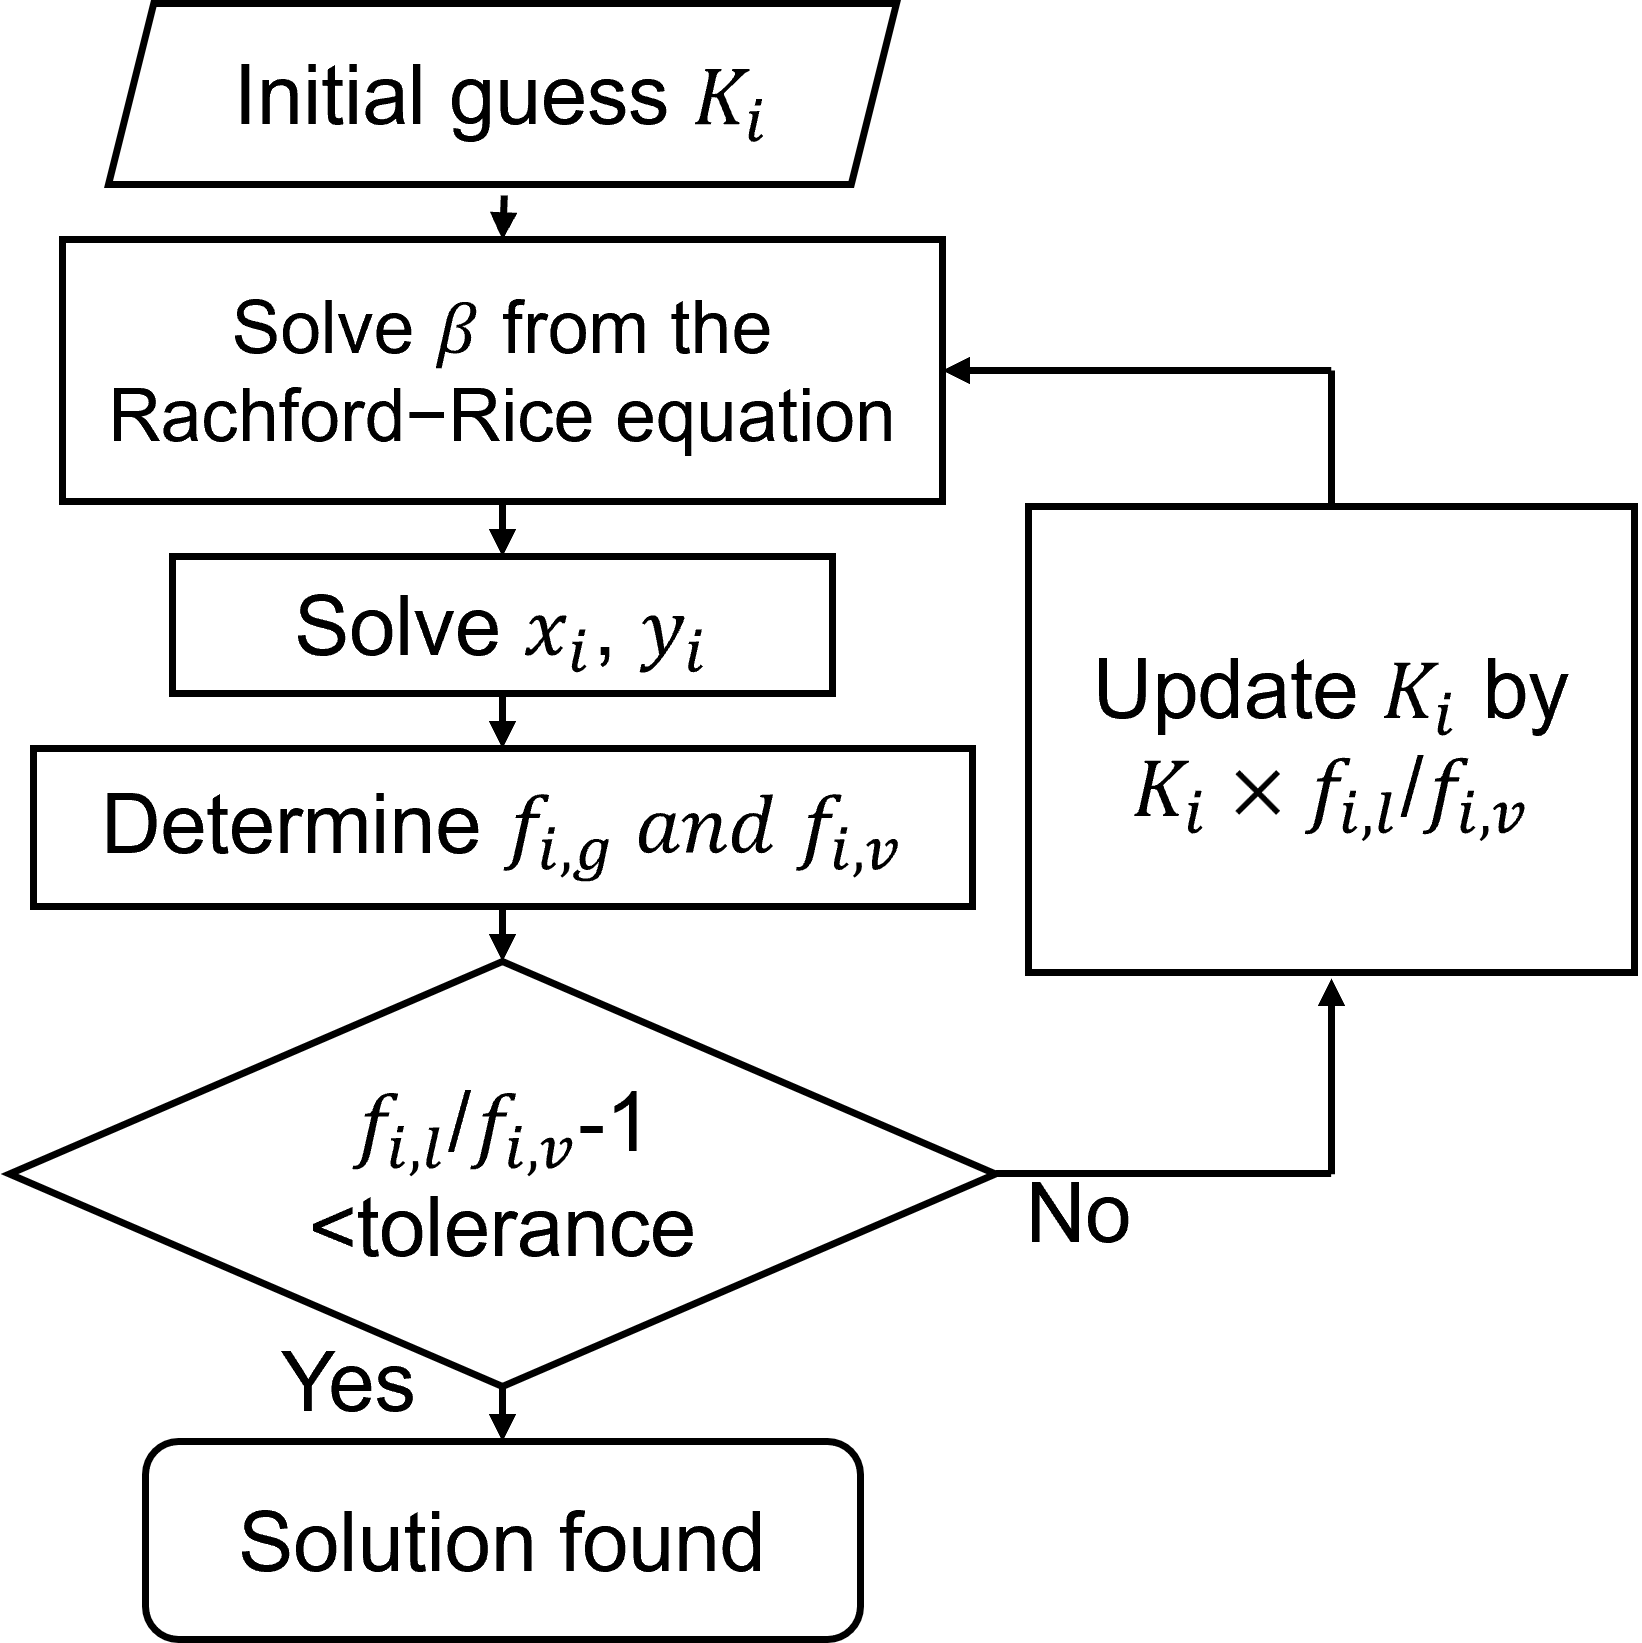
\includegraphics[width=0.35\linewidth]{TPn_flowchart.png}
\caption{Flow chart of TP flash solution process.}
\label{FC} 
\end{figure}

Once the initial guess is obtained, we proceed to solve the Rachford-Rice equation (Eq.~\ref{eq:5}) using the Newton-Raphson iteration method to determine the vapor mole fraction $\beta$. Subsequently, $x_i$ and $y_i$ can be calculated using Eqs.~\ref{eq:5-2}. The next step involves evaluating the fugacity using Eq.~\ref{fuga} and examining whether fugacity equilibrium has been achieved (i.e., $\left|f_{i,l}/f_{i,g}-1\right| < tol $). If equilibrium has not been reached, we update the equilibrium constant $K_i$ by multiplying it with the fugacity ratio $K_i=K_i \times f_{i,l}/f_{i,g}$ and then return to the step of solving the Rachford-Rice equation once again. This iterative process continues until the error falls below a specified tolerance $tol$, and $tol$ is $10^-8$ in this work. 


\textbf{PV flash and UV flash:}
The PV flash and UV flash solvers are developed based on the TP flash method, utilizing iteration methods. For both solvers, initial guesses (T for PV flash; T and P for UV flash) are obtained from the cell value in the previous time step, and a TP flash problem is solved in each iteration. During the iteration process, T and/or P are updated to find a better solution. After multiple iterations, when the error (PV flash error: $|\rho - \rho_0|$, UV flash error: $|e - e_0|$ and $|\rho - \rho_0|$) falls below a specified tolerance, the solver returns the solution of TP flash problem.


In the PV flash solver, as the pressure (P) is already provided as input, only the temperature (T) needs to be guessed and updated during the iteration. To avoid the computational cost of computing derivatives in the Newton-Raphson method, a secant method is employed to update T.


In contrast, the UV flash solver requires simultaneous guessing and updating of two variables,  temperature (T) and pressure (P), during the iteration. Therefore, the secant method cannot be directly applied. Instead, the Newton-Raphson method is used to solve UV flash problems. The required Jacobian matrix is obtained using the analytical framework described in Sec.~\ref{sec:analytical}.



\subsubsection{Models of transport properties}
To evaluate the dynamic viscosity and thermal conductivity at transcritical conditions, the dense fluid formulas (i.e., the Chung's method~\cite{chung1988generalized}) are used. This method gives accurate estimations of viscosity and thermal conductivity of polar, non-polar, and associating pure fluids and mixtures. In this method, dynamic viscosity and thermal conductivity have the similar formula:
\begin{equation}
\lambda=\lambda_0 \lambda^*+\lambda_p, \label{transp}
\end{equation}
where $\lambda$ represents dynamic viscosity or thermal conductivity. $\lambda_0$ is the property at the low-pressure limit. $\lambda^*$ and $\lambda_p$ are high pressure corrections. At high pressures, $\lambda_p$ is the major contributing term compared to $\lambda_0 \lambda^*$. On the other hand, at low pressures, $\lambda^*$ is approaching unity and the $\lambda_p$ term is negligible such that Eq.~\ref{transp} reduces to $\lambda_0$. Hence, the transition between low-pressure and high-pressure properties is smoothly described by the model. 

For mass diffusivity, we used a mixture-averaged mass diffusion model~\cite{kee1996chemkin}. The mass diffusion coefficient $D_i$ of specie $i$ is defined as
\begin{equation}
D_i=\frac{1-Y_i}{\sum^N_{j\neq i}z_j/D_{j,i}},\label{massdiff}
\end{equation}
where $Y_i$ and $z_i$ are the mass and mole fractions of component $i$, respectively; $D_{i,j}$ is the binary mass diffusion coefficient of component $i$ in component $j$, which is evaluated by Fuller’s model~\cite{fuller1966new} with Takahashi’s correction~\cite{takahashi1975preparation} for high pressures.


\subsection{VLE-based CFD framework}
\label{sec:model:cfd}
In this work, a transcritical multiphase flow solver is developed by coupling a density-based fully compressible CFD solver with several VLE solvers. 
The governing equations of the CFD solver are the multi-component transport equations, including the mixture density equation (i.e., continuity equation), mixture momentum equations, mixture internal energy equation, and 
component mass fraction equation as follows:
\begin{align}
 &\frac{\partial \rho}{\partial t}+\frac{\partial \rho u_i}{\partial x_i}=0 \label{Gc},\\
 &\frac{\partial \rho u_i}{\partial t}+\frac{\partial \rho u_i u_j}{\partial x_j}=-\frac{\partial P}{\partial x_i}+\frac{\partial \tau_{ij}}{\partial x_j} \label{Gm},\\
 &\frac{\partial \rho e}{\partial t}+\frac{\partial \rho u_i e}{\partial x_i}+\frac{\partial \rho K}{\partial t}+\frac{\partial \rho u_i K}{\partial x_i}+\frac{\partial  u_i P}{\partial x_i}=-\frac{\partial q_i}{\partial x_i} +\frac{\partial \tau_{ij}u_j}{\partial x_i},\\
  &\frac{\partial \rho Y_m}{\partial t}+\frac{\partial \rho Y_m u_i}{\partial x_i}=\frac{\left(\rho Y_m V_{mi}\right)}{\partial x_i},
  %\frac{\partial }{\partial x_j}\left(\rho D \sum_m h_m \frac{\partial Y_m}{\partial x_j}\right)-\frac{\partial }
\end{align}
where $u_i$ is the velocity, $\rho$ is mixture density, $e$ is specific internal energy, $Y_m$ is the mass fraction of specie $m$, $\tau_{ij}$ is the viscous stress tensor defined by $ \tau_{ij} = -\frac{2}{3}\mu\frac{\partial u_k}{\partial x_k}\delta_{ij} + \mu \left( \frac{\partial u_i}{\partial x_j} +\frac{\partial u_j}{\partial x_i}\right) $, $K$ is the kinetic energy, and $q_i$ is the heat flux. $q_i = -\kappa \nabla  T$ where $\kappa$ is the thermal conductivity. 
The Fickian diffusion is used to evaluate the diffusion velocity in the governing equations:

$$ V_{mi} = -\frac{D_m}{X_m}\frac{\partial X_m} {\partial x_i} + \sum^{N}_{s}\frac{Y_s D_s}{X_s}\frac{\partial X_s} {\partial x_i},$$
where $X_m$, and $D_m$ are the mole fraction and the mixture-averaged diffusion coefficient of specie $m$, respectively. $M$ is the total molar mass. The second correction term is to ensure global mass conservation $\sum^{N}_{m} \rho Y_m V_m = 0$.


The CFD solver was developed based on the central-upwind scheme \cite{kurganov2001semidiscrete,greenshields2010implementation}. At each time step, the conservative variables $\rho$, $\rho u$, $\rho e$, and $\rho Y_m$ are updated according to the governing equations. The central upwind scheme mentioned is a fully conservative (FC) method. 

To eliminate spurious pressure oscillations, a quasi-conservative approach called the double flux (DF) method \cite{abgrall2001computations,billet2003adaptive,ma2017entropy} is also implemented.
This method locally freezes the real fluid properties to those of an equivalent calorically perfect gas. During the calculation of the new time step, in each cell, a local calorically perfect-gas EOS is defined using the thermodynamic properties. The pressure field is updated using this newly defined EOS, effectively mitigating the occurrence of spurious pressure oscillations. Subsequently, the remaining thermodynamic properties such as density and species mass fraction are updated using the real-gas EOS and PV flash based on the updated pressure, density, and species mass fraction values. The use of a calorically perfect-gas EOS in the double flux method has been shown by Ma et al. to successfully remove spurious pressure oscillations \cite{ma2017entropy}. To define a locally calorically perfect-gas EOS, an effective specific heat ratio $\gamma^*$ and an effective internal energy $e_0^*$  are formulated as:
\begin{align}
\gamma^*& = \frac{\rho c^2}{P},&e_0^*&= e-\frac{Pv}{\gamma^*-1},
\end{align}
where $c$ is the speed of sound, and $v$ is the specific volume. %$\gamma^*$ and $e_0^*$ can be calculated from the density, internal energy, and speed of sound, which are obtained from real gas EOS.
With real-fluid EOS, $\gamma^*$ and $e_0^*$ can be nonlinear functions of the thermodynamic states and may not be constant. The main idea of the double flux method is to freeze $\gamma^*$ and $e_0^*$ in space during each time step advancement. When calculating a flux of a face of a certain cell, the state variable used is not directly from the cell values but reconstructed using $\gamma^*$, $e_0^*$, $P$, and $\rho$. Although this face also belongs to the adjacent cell, its $\gamma^*$, $e_0^*$ of the adjacent cell are not used.  For example, on a one-dimensional mesh, the numerical face flux $F^L_{i+\frac{1}{2}}$ for the cell $i$ at $x_{i+\frac{1}{2}}$ can be expressed as (see Fig.~\ref{DF_CFD})
\begin{align}
F^L_{i+\frac{1}{2}}& = F\left(U^L_{i+\frac{1}{2}},U^R_{i+\frac{1}{2}}\right),&
U^L_{i+\frac{1}{2}}& = U^L\left(\gamma^*_i,e_{0,i}^*,P,\rho ,Y\right) ,&
U^R_{i+\frac{1}{2}}& = U^R\left(\gamma^*_i,e_{0,i}^*,P,\rho ,Y\right),
\end{align}
where $U^L$ and $U^R$ are conservative variables constructed using calorically perfect-gas EOS. The stencil for constructing conservative variables depends on the interpolation scheme, and the vanLeer method \cite{van1974towards} is used in the current work. In the central-upwind method,

\begin{align} F^L_{i+\frac{1}{2}} &= \alpha u^LU^L + \left(1-\alpha\right)u^R U^R + \omega \left(U^R-U^L\right),&
\alpha &= \frac{\phi^L}{\phi^L +\phi^R},&
 \omega &= \alpha \left(1-\alpha\right) \left(\phi^L+\phi^R\right)
 \end{align}
\begin{align} \phi^L& = max\left(c^L+|u^L|,c^R + |u^R|,0\right),&\phi^R &= max\left(c^L-|u^L|,c^R - |u^R|,0\right)
\end{align}

where $c$ and $u$ are the speed of sound and velocity respectively. They are obtained from the same interpolation scheme.


In this way, the $\gamma^*$ and $e_0^*$ are frozen, and the fluid is locally calorically perfect to remove spurious pressure oscillation. 
Since each face is adjacent to two cells, the two fluxes (i.e., the left flux $F^L_{i+\frac{1}{2}}$ and the right flux $F^R_{i+\frac{1}{2}}$ in Fig.~\ref{DF_CFD}) obtained from two cells can be different. That is why this method is called ``double flux'', and where two fluxes are different, the numerical scheme is no more conservative. 
\begin{figure*}[htbp]
\centering
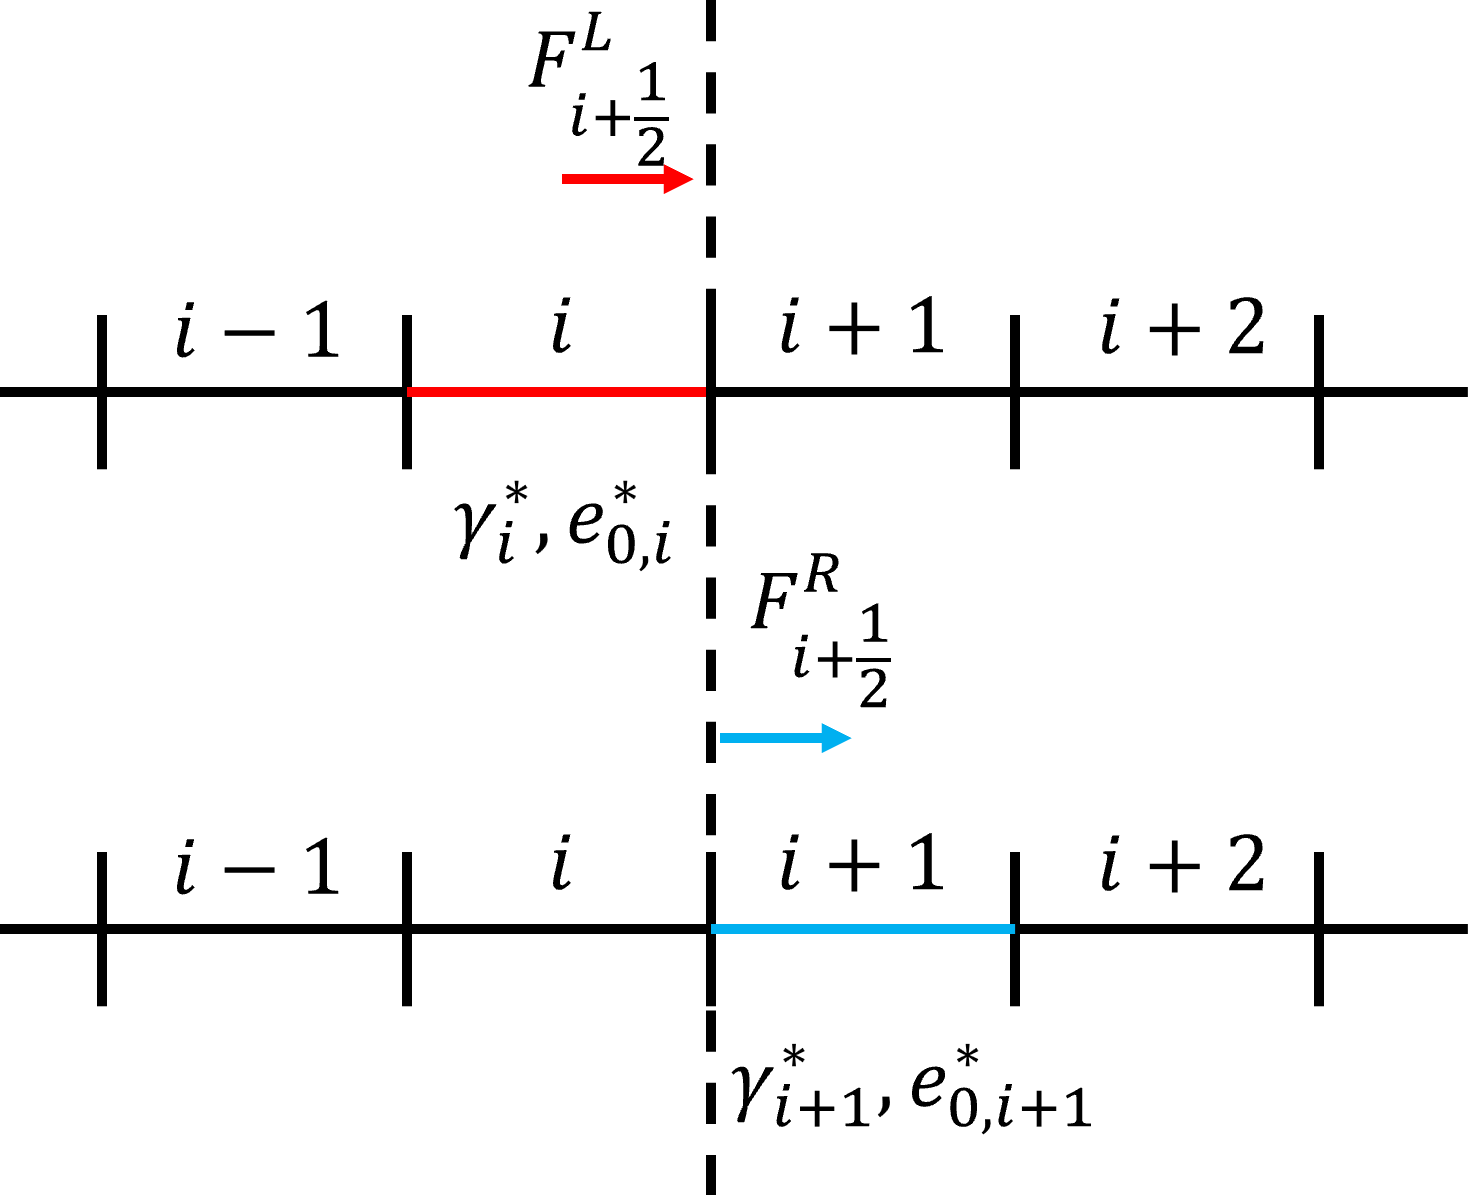
\includegraphics[width=0.4\linewidth]{DF.png}
\caption{Schematic of the double flux (DF) method in a one-dimensional mesh.}
\label{DF_CFD} 
\end{figure*}

At each time step, $\rho$, $u$, and $Y_m$ are updated using the central-upwind scheme. Then, the DF method is used to update $e$ and $P$. After that, $T,\beta,c$ are obtained using the PV flash solver. For the fully conservative scheme (without DF method), $P,T,\beta,c$ are directly updated using the UV flash solver. This entire process is shown in Fig.~\ref{FC_CFD}. DF method is useful to solve the system with large density gradient, but since it is not an energy-conservative scheme, it could cause other problems. In Sec.~\ref{sec:DF}, we compared the results of two methods, and discuss their pros and cons.

\begin{figure*}[htbp]
\centering
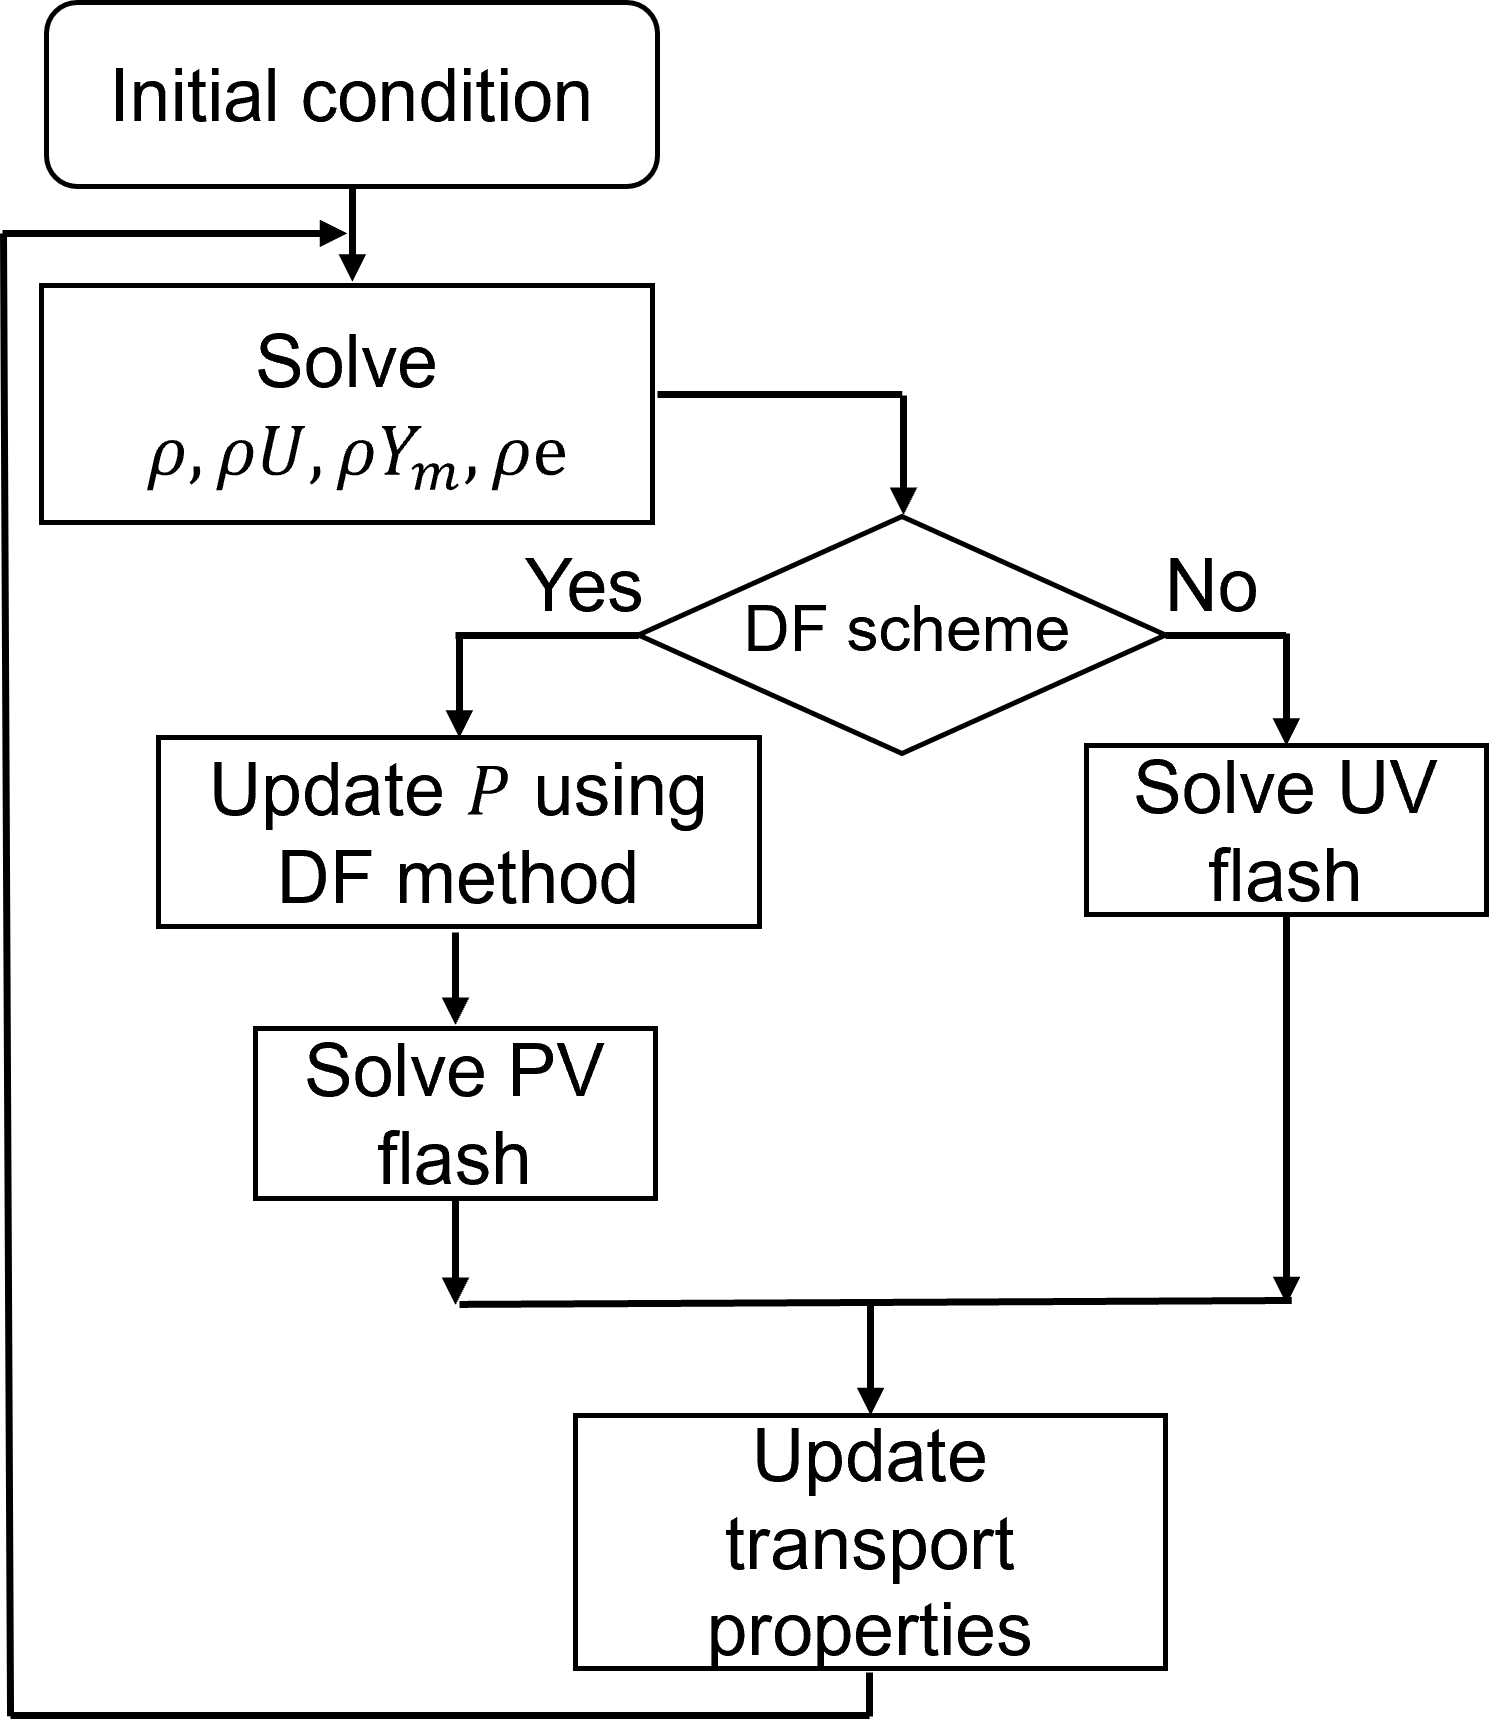
\includegraphics[width=0.4\linewidth]{solver_flow_chart.png}
\caption{Flow chart of the VLE-based CFD framework.}
\label{FC_CFD} 
\end{figure*}

\subsection{\textit{In Situ} Adaptive Tabulation (ISAT)}
\label{sec:ISAT}
The \textit{n situ} adaptive tabulation (ISAT) method, originally introduced by Pope \cite{pope1997computationally}, offers an effective approach to reduce the computational cost associated with detailed chemistry calculations. In contrast to traditional tabulation methods that require pre-processing to generate tables before the CFD simulation, ISAT dynamically constructs the table during the simulation itself. This dynamic construction enables us to store only the necessary records, significantly reducing the table size and mitigating the curse of dimensionality. During the CFD simulation, most of the queries can be efficiently retrieved by utilizing linear approximation based on the table records, eliminating the need for direct calculations. This approach not only enhances computational efficiency but also ensures that the results are obtained with a high degree of accuracy. ISAT's ability to provide excellent error control contributes to maintaining the desired level of precision. Given these advantages, employing the ISAT method to tabulate VLE solutions proves to be a promising strategy for accelerating VLE-based CFD simulations.

%The fluid solver directly updates pressure $P$, enthalpy $h$, and mass mole fraction of every component $Y_m$ from the governing equation, and require thermodynamic model to evaluate temperature $T$, and gas mole fraction $\psi_g$ and speed of sound $c$. ($T$,$\psi_g$) can be solved by PHn flash solver, $c$ is obtained from analytical approach \cite{tudisco2020analytical}. 
The relation between the given condition $\boldsymbol{x}$ and solution $\boldsymbol{y}$ of a VLE solver can be denoted as a function or mapping $\boldsymbol{F}$:
$$\boldsymbol{y=F\left(x\right)}.$$
Specifically, certain variables are required for the implementation of the FC and DF schemes. Firstly, the speed of sound $c$ is required to ensure the accuracy and stability of the solver. Additionally, the vapor mole fraction $\beta$ is used for capturing phase separation. $c$ and $\beta$ are two output variables needed by all VLE solvers. The input and other output variables are determined by the flash solver. For the PV flash solver, the input variables consist of the pressure ($P$), density ($\rho$), and mole fractions ($z_i$) of each component in the mixture. The solver then provides the following output variables: temperature ($T$), specific internal energy ($e$), speed of sound ($c$), and vapor mole fraction ($\beta$).
On the other hand, the UV flash solver takes as input the specific internal energy ($e$), density ($\rho$), and mole fractions ($z_i$). It then calculates and provides the output variables of temperature ($T$), pressure ($P$), speed of sound ($c$), and vapor mole fraction ($\beta$).

%Specifically, due to the need for the central upwind scheme, the CFD solver requires speed of sound $c$. And vapor mole fraction $\beta$ is also needed to capture phase separation. And the input and other output variables are determined by the flash solver. For PV flash solver, the input is $\left(P,\rho,z_i\right)$, where $z_i$ mole fraction of component $i$ in the total mixture, and the output $\left(T,e, c, \beta\right)$, where $e$ is specific internal energy, required by double flux. For UV flash solver, the input is  $\left(e,\rho,z_i\right)$, and  the output is $\left(T,P, c, \beta\right)$.

For every record in the table, it contains $(\mathbf{x}_0,\mathbf{y}_0,\left.\frac{\partial  \mathbf{F}}{\partial \mathbf{x}}\right|_{\mathbf{x}_0}, \mathbf{M})$. 
The gradient (i.e., Jacobian matrix $\left.\frac{\partial  \mathbf{F}}{\partial \mathbf{x}}\right|_{\mathbf{x}_0}$) is evaluated analytically (in Sec.~\ref{sec:analytical}) and used for local linear approximation:
$$\mathbf{y}\approx\mathbf{y}_{linear}=\mathbf{y}_0+\left.\frac{\partial  \mathbf{F}}{\partial \mathbf{x}}\right|_{\mathbf{x}_0}\cdot\left(\mathbf{x}-\mathbf{x}_0\right).$$
The matrix $\mathbf{M}$ is used to define the region of accuracy (ROA), in which the local error
$\mathbf{\epsilon}$ does not exceed the tolerance $\mathbf{\epsilon}_{tol}$. The ROA is defined by an inequality:
$$\left(\mathbf{x}-\mathbf{x}_0\right)^T \mathbf{M} \left(\mathbf{x}-\mathbf{x}_0\right) \leq 1.$$
The region satisfying this inequality is a hyper-ellipsoid, and hence the ROA is also called Ellipsoid of Accuracy (EOA), as shown in Fig.~\ref{ISAT_ROA}.
\begin{figure}[htbp]
    \centering
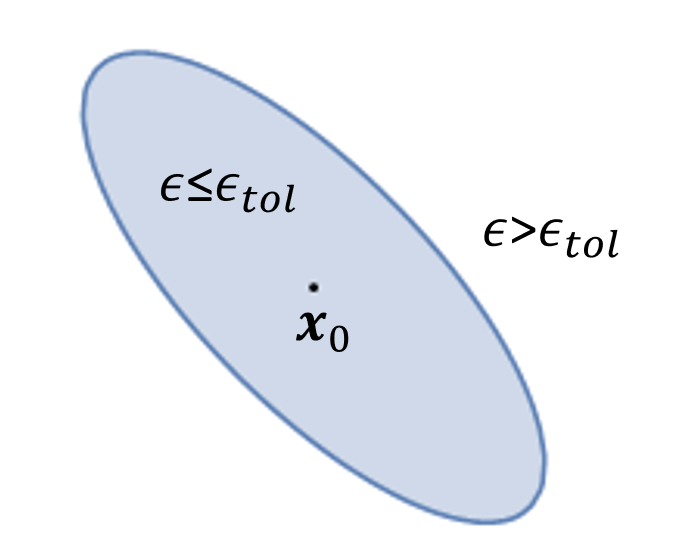
\includegraphics[width=0.20\linewidth]{Region of accuracy.png} 
\caption{Sketch of region of accuracy (ROA).}
\label{ISAT_ROA} 
\end{figure}
For initial setting, the linear term $\left.\frac{\partial  \mathbf{F}}{\partial \mathbf{x}}\right|_{\mathbf{x}_0}\cdot\left(\mathbf{x}-\mathbf{x}_0\right)$ is considered as an error. So, the initial $\mathbf{M}$ can be set as 
$$\mathbf{M}=\left(\left.\frac{\partial  \mathbf{F}}{\partial \mathbf{x}}\right|_{\mathbf{x}_0}\right)^T \left(\left.\frac{\partial  \mathbf{F}}{\partial \mathbf{x}}\right|_{\mathbf{x}_0}\right)/\epsilon_{tol}^2.$$


\begin{figure}[htbp]
\centering
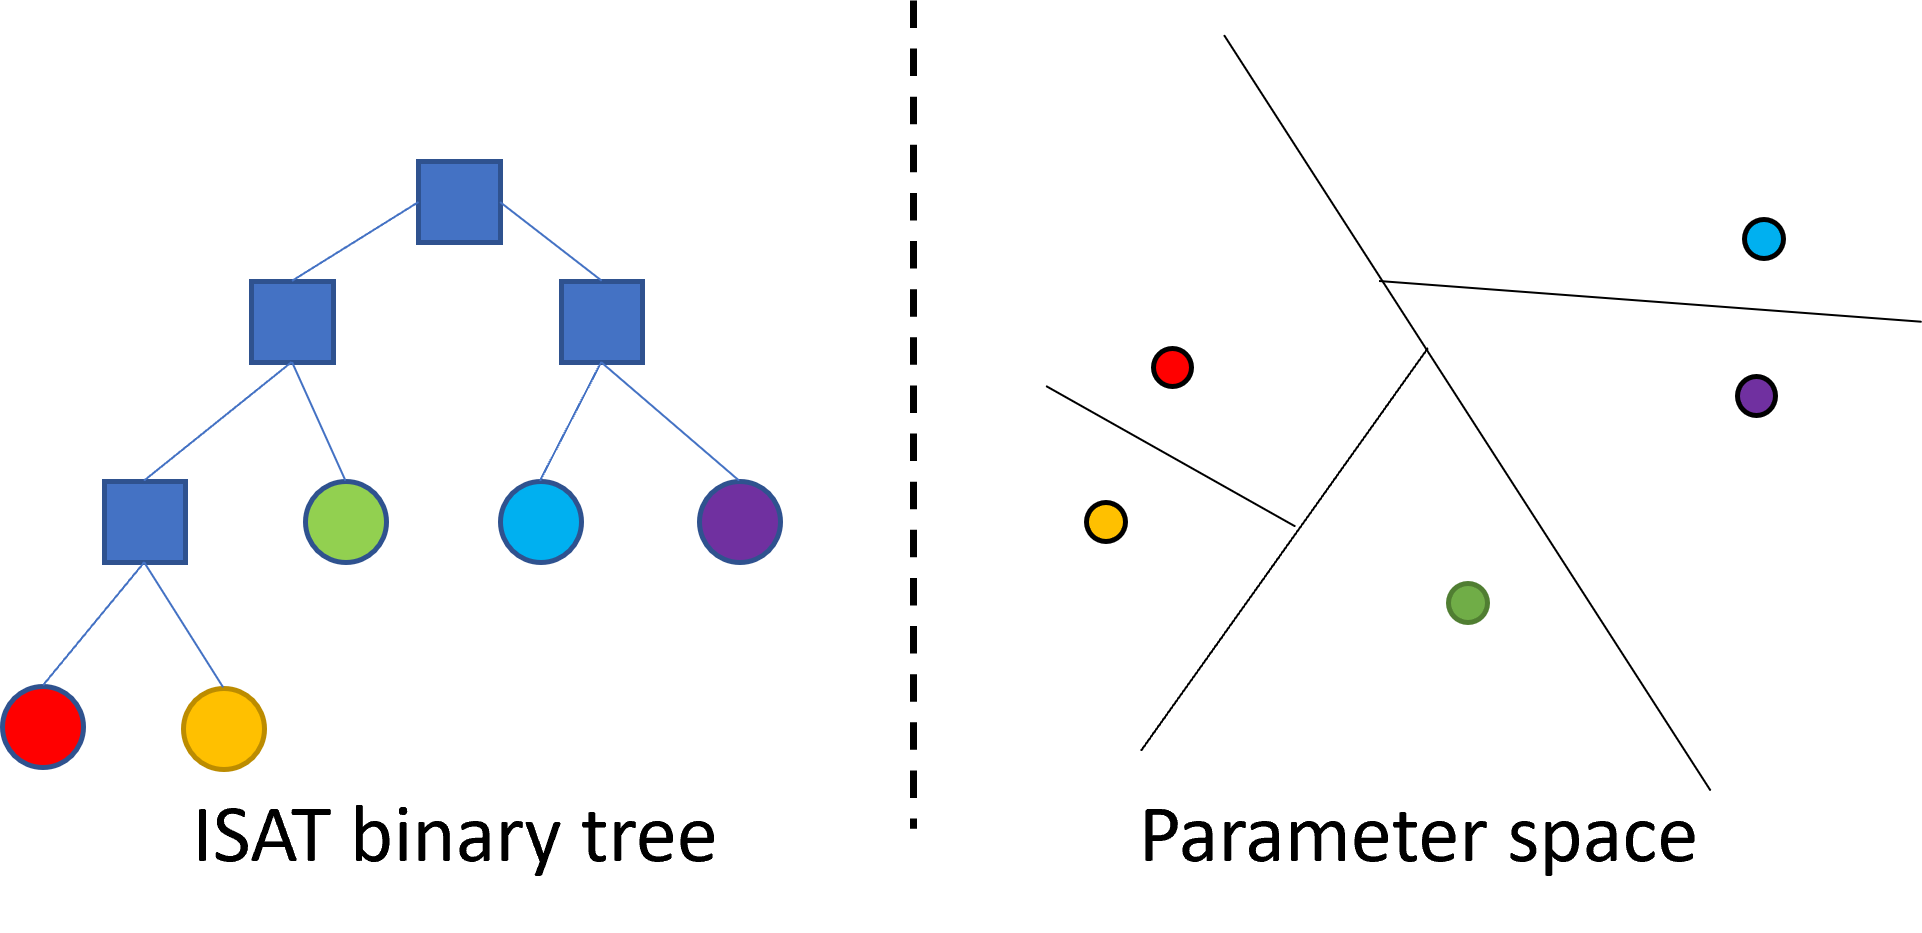
\includegraphics[width=0.6\linewidth]{ISAT tree.png}
\caption{The binary tree used to manage records in ISAT}
\label{ISAT_tree} 
\end{figure}
The management of records in the ISAT method is facilitated through a binary tree structure, as illustrated in Fig.~\ref{ISAT_tree}. Each node of the tree stores a vector that defines a hyperplane, dividing the parameter space into two distinct half-spaces. The data corresponding to each half-space is stored in the respective sub-trees. By employing this tree structure, the entire parameter space can be divided into numerous small cells, with the records being stored at the leaf nodes. During the search operation, at each layer of the tree, the sub-tree is selected based on which half-space contains the input parameter. This process continues until the desired record is found. It is important to note that the record obtained through this method may not be the closest to the input data. Nevertheless, this approach is simple and efficient enough to satisfy the requirements of the simulation. When it comes to the insertion operation, a new node is created, and its hyperplane is defined using the median plane of a table record (obtained from the search operation) and the record being inserted. The ISAT binary tree is not a balanced tree.  Consequently, during simulations, a large number of records may be concentrated in one of the two sub-trees, resulting in an increased height of the tree structure. This can negatively impact the performance of lookup and insertion operations. To prevent such degradation, a rebuilding process is implemented. Specifically, at every 20 time steps, if the tree height exceeds twice the height of a perfectly balanced tree, a new tree structure is constructed using the existing records to restore perfect balance and optimize performance.



In a simulation, for the first query, a new record is calculated and added to the table. 
For subsequent queries $(\mathbf{x}_{new})$, the closest record $(\mathbf{x}_0,\mathbf{y}_0,\left.\frac{\partial \mathbf{F}}{\partial \mathbf{x}}\right|_{\mathbf{x}_0}, \mathbf{M})$ is searched out, and then one of the following three operations is conducted, as shown in Fig.~\ref{ISAT_ALG}:

(1) \textbf{Retrieval}: If $\mathbf{x}_{new}$ is within the EOA of the record, then the linear approximation $\mathbf{y}_{linear}$ is returned. Otherwise $\mathbf{y}_{new}=\mathbf{F}\left(\mathbf{x}_{new}\right)$ is calculated. 

(2) \textbf{Growth}: If $\left|\mathbf{y}_{new}- \mathbf{y}_{linear}\right|\leq\epsilon_{tol}$, then EOA is grown to include $\mathbf{x}_{new}$. Specifically, the new EOA is the smallest ellipsoid covering both the old EOA and $\mathbf{x}_{new}$. $\mathbf{y}_{new}$ is returned.

(3) \textbf{Addition}: Otherwise $\left|\mathbf{y}_{new}- \mathbf{y}_{linear}\right|>\epsilon_{tol}$, then new record is added to the table, and $\mathbf{y}_{new}$ is returned.

\begin{figure}[htbp]
\centering
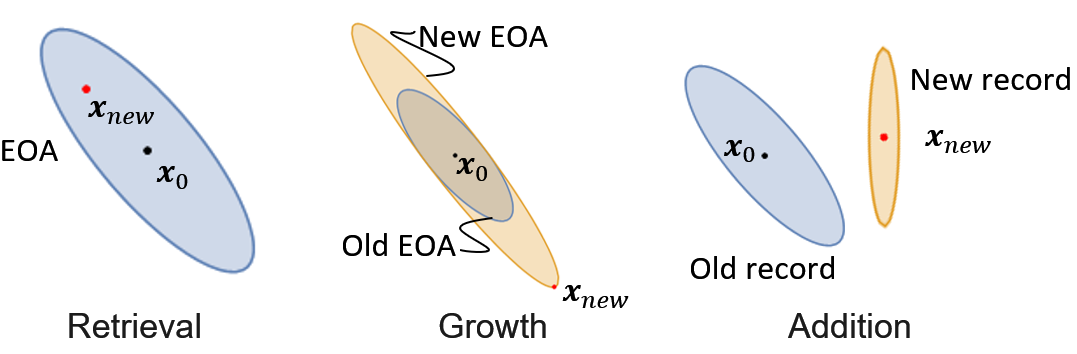
\includegraphics[width=0.6\linewidth]{s.png}
\caption{Sketch showing the three operations in the ISAT method.}
\label{ISAT_ALG} 
\end{figure}

In the ISAT method, a maximum number of records are set due to the limitation of memory. When the number of records reaches the maximum, the table is full, and new addition actions can't be taken. In L. Lu and S.B Pope's work \cite{lu2009improved}, they compared three actions: (a) don't add the new record to the table; (b) remove the least recently used record; (c) remove the least frequently used record. They claimed that for non-stationary problems, (b) is likely optimal. They maintain a linked list (called MFU list in \cite{lu2009improved}) to obtain the least recently used record. In the list, the records are in the order in which they have most frequently been used. We follow their idea (b) and further improve the method to remove records.

In our tests, we realized that the height of the binary tree becomes larger when there are more records, making the search slower. Moreover, in the non-stationary simulation, a large number of records are required only in a certain time interval, after which many records are redundant and only degrade the performance of the search. These redundant records should be accurately detected and quickly deleted to improve performance. We propose two methods, 
\begin{itemize}
\item delete data that has not been used in the last few time steps. 
\item use an adaptive table maximum size, and the size is formulated as:
\end{itemize}
\begin{align}
N_{max} = C \sum_{i=0}^M  N_{\text{inactive},i}  \label{eq:adap}
\end{align}
where $ N_{\text{inactive},i}$ is the number of records of which the last call was $i$ time steps ago. $M$ is the number of time steps considered and $C$ is a multiplier ($C>1$). $M$ and $C$ are tunable parameters.


We propose a new data structure to support the proposed methods. The data structure is a list of linked lists, shown in Fig.~\ref{ISAT_LL}. It has multiple layers (4 layers in Fig.~\ref{ISAT_LL}), $T_1$ stores the records just used in the previous time step, $T_2$ stores the records used in the time step before the previous time step, and so on and so forth. $T_4$ has all records not been used within 3 latest time steps. With this list, all records are sorted according to the distance between the current time step and the time step of the last call, and the proposed deletion methods can be efficiently implemented. The main list ($T_1-T_4$ list) is a circular array, the list head is the layer of the most recently used records and the tail is the layer of the least recently used records. In a new time step, the linked list of the tail ($T_4$) is merged with the previous layer ($T_3$), and this empty layer ($T_4$) becomes the new head, and all records called during this time step will insert into this layer. The previous layer ($T_3$) becomes the new tail. Since we use a combination of a circular array and linked lists, the above operations can be accomplished achieved with O(1) time complexity.

\begin{figure}[htbp]
\centering
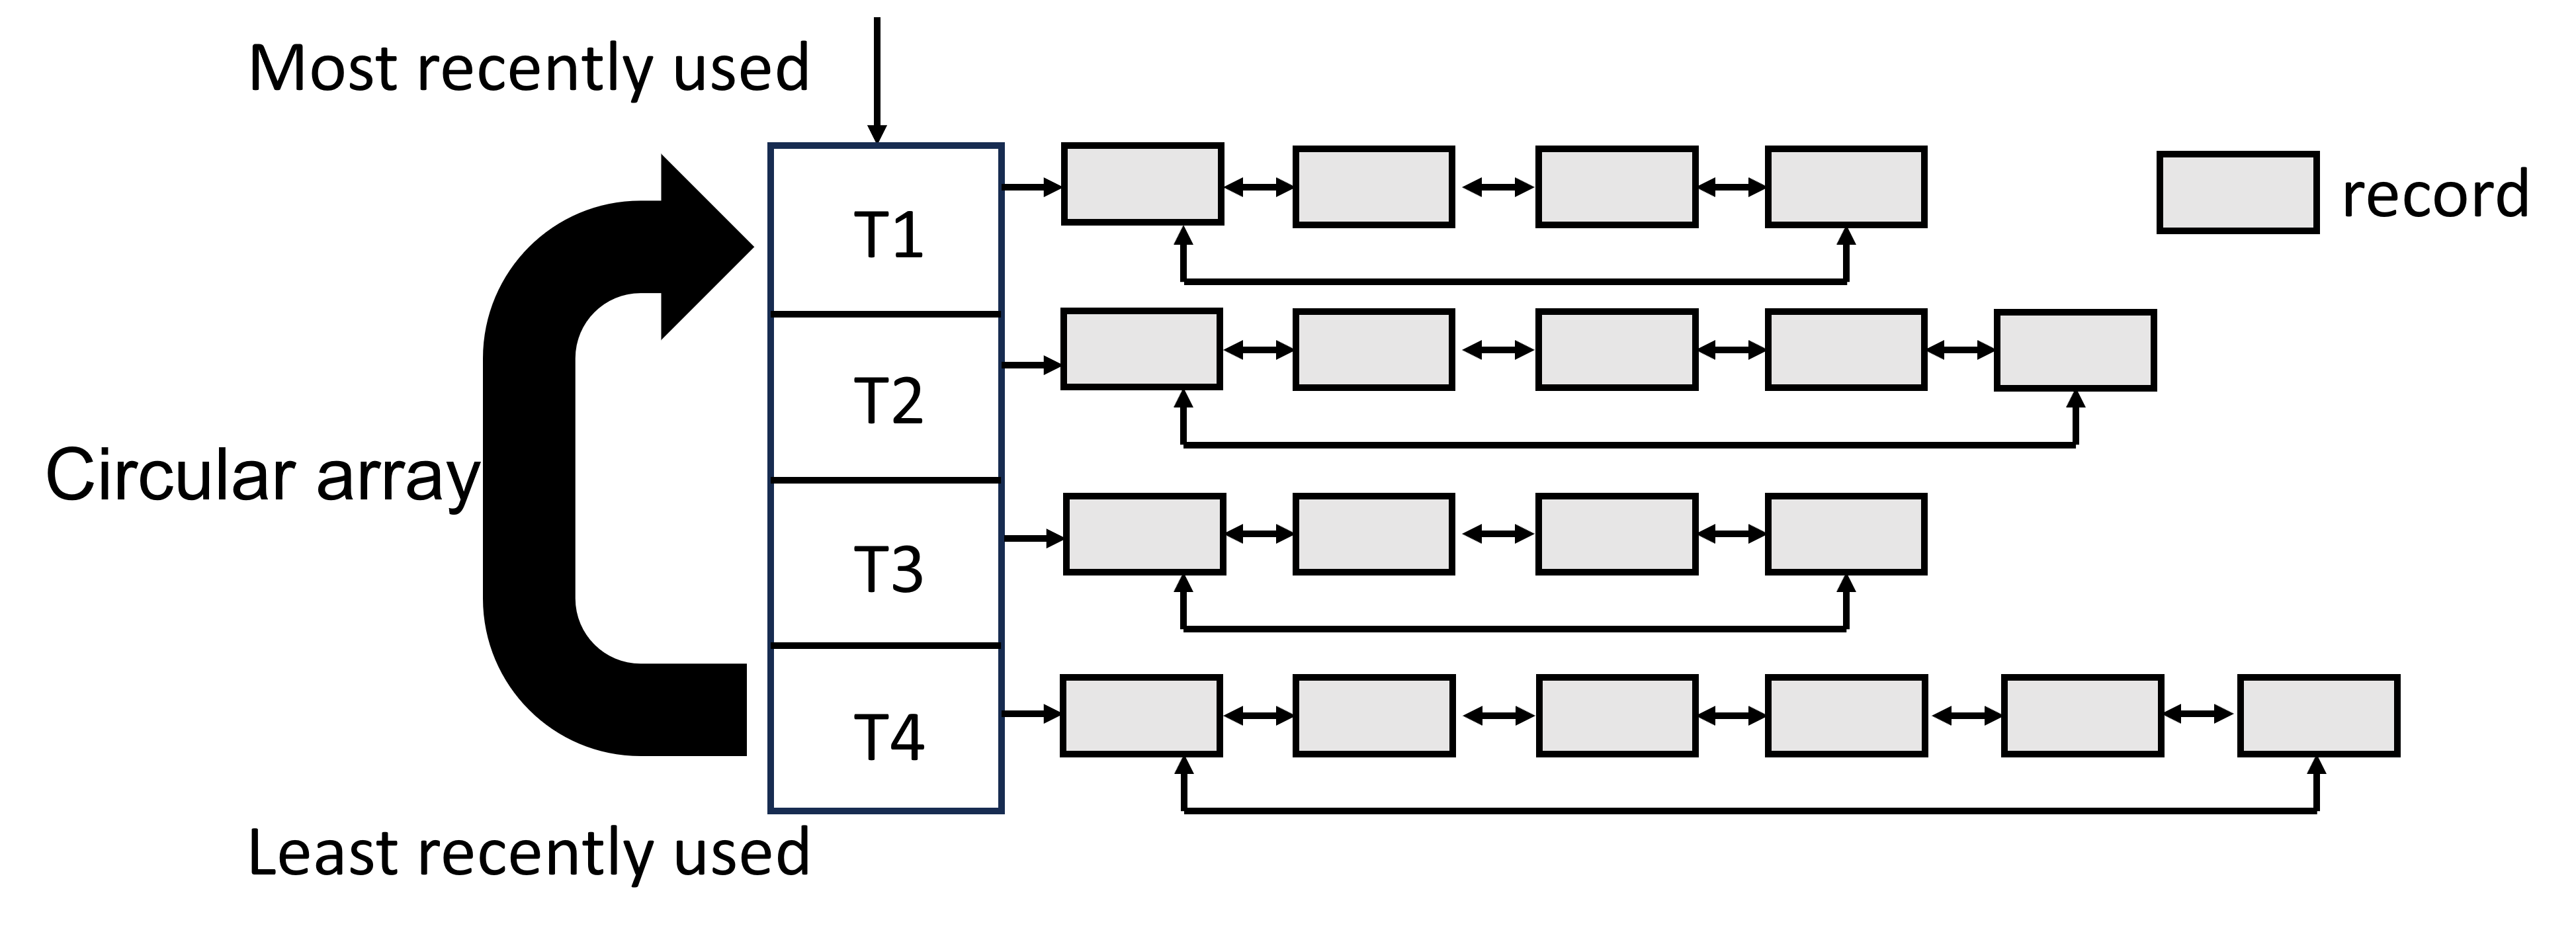
\includegraphics[width=0.6\linewidth]{linkedlist2.png}
\caption{schematic of the data structure to support methods for removing redundant records}
\label{ISAT_LL} 
\end{figure}

\subsection{Analytical framework for VLE}
\label{sec:analytical}

The first-order derivatives of thermodynamic properties considering phase change are required when calculating the speed of sound (Eq.~\ref{eq:soundspeed}), solving the VLE system (e.g., using the Newton-Raphson iteration method), and using the ISAT-VLE method (e.g., evaluating the Jacobian matrix $\left.\frac{\partial  \mathbf{F}}{\partial \mathbf{x}}\right|_{\mathbf{x}_0}$). These derivatives can be obtained numerically by a perturbation method, which is more computationally expensive and introduces additional errors. Most importantly, profiles of thermodynamic properties can have discontinuities/jumps at the phase boundaries, and hence the numerical derivatives from the perturbation method can be incorrect and diverge the simulation. To address all the above challenges, We developed an analytical method to evaluate the required derivatives.
In order to calculate the derivatives of thermodynamic properties considering phase change, after obtaining a few derivatives listed below, the calculation can be finished using a simple framework.
\begin{align}
\left(\frac{\partial x_k}{\partial T}\right)_{P,\mathbf{z}},\left(\frac{\partial y_k}{\partial T}\right)_{P,\mathbf{z}},\left(\frac{\partial x_k}{\partial P}\right)_{T,\mathbf{z}},\left(\frac{\partial y_k}{\partial P}\right)_{T,\mathbf{z}},\left(\frac{\partial x_k}{\partial z_i}\right)_{T,P,z_{s,s\neq i}},\left(\frac{\partial y_k}{\partial z_i}\right)_{T,P,z_{s,s\neq i}}
\end{align}
The formula of these terms is provided in Appendix ~\ref{App:VLE}, and its derivation is based on Tudisco and Menon's work \cite{tudisco2020analytical}.
For single-phase properties, the temperature and pressure derivatives can be obtained using the chain rule:
\begin{align}
\left(\frac{\partial (\cdot)_l}{\partial T}\right)_{P,\mathbf{z}} = \left(\frac{\partial (\cdot)_l}{\partial T}\right)_{P,\mathbf{x}} + \sum_{k=1}^N\left(\frac{\partial (\cdot)_l}{\partial x_k}\right)_{P,T,x_{s,s\neq k}}\left(\frac{\partial x_k}{\partial T}\right)_{P,\mathbf{z}} \label{eq:dvdT}
\end{align}
\begin{align}
\left(\frac{\partial (\cdot)_v}{\partial T}\right)_{P,\mathbf{z}} = \left(\frac{\partial (\cdot)_v}{\partial T}\right)_{P,\mathbf{y}} + \sum_{k=1}^N\left(\frac{\partial (\cdot)_v}{\partial y_k}\right)_{P,T,y_{s,s\neq k}}\left(\frac{\partial y_k}{\partial T}\right)_{P,\mathbf{z}} \label{eq:dldT}
\end{align}
The pressure derivatives use similar formulas with all the $\left(\frac{\partial (\cdot)}{\partial T }\right)$ replaced by $\left(\frac{\partial (\cdot)}{\partial P }\right)$.

The $z$ derivatives are formulated as:
\begin{align}
\left(\frac{\partial (\cdot)_l}{\partial z_i}\right)_{P,T} =  \sum_{k=1}^N\left(\frac{\partial (\cdot)_l}{\partial x_k}\right)_{P,T,x_{s,s\neq k}}\left(\frac{\partial x_k}{\partial z_i}\right)_{P,T,\mathbf{z}} \label{eq:dldz}
\end{align}

\begin{align}
\left(\frac{\partial (\cdot)_v}{\partial z_i}\right)_{P,T} =  \sum_{k=1}^N\left(\frac{\partial (\cdot)_v}{\partial x_k}\right)_{P,T,x_{s,s\neq k}}\left(\frac{\partial y_k}{\partial z_i}\right)_{P,T,\mathbf{z}} \label{eq:dvdz}
\end{align}

Note that the derivatives such as $\left(\frac{\partial (\cdot)_v}{\partial T}\right)_{P,\mathbf{y}}$,$\left(\frac{\partial (\cdot)_v}{\partial P}\right)_{T,\mathbf{y}}$, $\left(\frac{\partial (\cdot)_v}{\partial y_k}\right)_{P,T,y_{s,s\neq k}}$, are single-phase derivatives, and no phase change calculation is involved. These terms can be directly obtained by taking derivatives of the analytical form of EOS (including the departure functions derived from EOS) and NASA Polynomials. 


In TP flash, the thermodynamic properties are considered as a function of mixture temperature $T$, pressure $P$, and composition $\mathbf{z}$. The first-order derivatives are required by TP flash calculation (e.g., using the Newton-Raphson iteration method) and also the ISAT of TP flash solutions (e.g., evaluating the Jacobian matrix $\left.\frac{\partial  \mathbf{F}}{\partial \mathbf{x}}\right|_{\mathbf{x}_0} = \left.\frac{\partial  \left(\rho, e, \beta, c\right)}{\partial \left(P,T,\mathbf{z}\right)}\right|_{\mathbf{x}_0}$).
First, the derivative of $\beta$ is formulated as: (details are shown in Appendix~\ref{App:VLE})

\begin{align}
\left(\frac{\partial \beta }{\partial T}\right)_{P,\mathbf{z}} = \sum_{k=1}^N \left(\frac{\partial v_k}{\partial T}\right)_{P,\mathbf{z}},\left(\frac{\partial \beta}{\partial P}\right)_{T,\mathbf{z}} = \sum_{k=1}^N \left(\frac{\partial v_k}{\partial P}\right)_{T,\mathbf{z}}, \left(\frac{\partial \beta}{\partial z_i}\right)_{T,P,z_{s,s\neq i}}=\sum_{j=1}^N\left(\frac{\partial N_{j,v}}{\partial N_i}\right)_{T,P,N_{s,s\neq j}} -\beta
\end{align}
where $v_k$ is the mole fraction of component $k$ in the vapor phase of the total mixture ($v_k = \beta y_k$), 
$N_i$ is the total number of moles of component $i$ in the mixture, and $N_{k,v}$ are the number of moles of component $k$ in vapor phase.

The derivative of $\rho$ and $e$ are obtained from Eq.~\ref{eq:rho} and Eq.~\ref{eq:e}.
\begin{align}
\left(\frac{\partial \rho}{\partial T} \right)_{P,\mathbf{z}}= 
- \frac{\rho^2}{M}\Bigg\{\left(\frac{\partial \beta}{\partial T}\right)_{P,\mathbf{z}}\left(\frac{M_v}{\rho_v}-\frac{M_l}{\rho_l}\right) + 
\frac{\beta}{\rho_v^2}\left[\rho_v\left(\frac{\partial M_v}{\partial T} \right)_{P,\mathbf{z}}-M_v \left(\frac{\partial \rho_v}{\partial T} \right)_{P,\mathbf{z}}\right] \\+
\frac{1-\beta}{\rho_l^2}\left[\rho_l\left(\frac{\partial M_l}{\partial T} \right)_{P,\mathbf{z}}-M_l \left(\frac{\partial \rho_l}{\partial T} \right)_{P,\mathbf{z}}\right]\Bigg\} 
\end{align}
\begin{align}
\left(\frac{\partial e}{\partial T}\right)_{P,\mathbf{z}}= \frac{1}{M}\left\{ \left(\frac{\partial \beta}{\partial T}\right)_{P,\mathbf{z}} \left(M_v e_v-M_l e_l\right)+\beta \left[e_v\left(\frac{\partial M_v}{\partial T}\right)_{P,\mathbf{z}}+M_v\left(\frac{\partial e_v}{\partial T}\right)_{P,\mathbf{z}}\right]\right.\\ \left.+\left(1-\beta\right)\left[e_l\left(\frac{\partial M_l}{\partial T}\right)_{P,\mathbf{z}}+M_l\left(\frac{\partial e_l}{\partial T}\right)_{P,\mathbf{z}}\right]\right\}
\end{align}
The derivatives of single phase properties such as $\left(\frac{\partial e_v}{\partial T}\right)_{P,\mathbf{z}}$,$\left(\frac{\partial M_v}{\partial T}\right)_{P,\mathbf{z}}$,$\left(\frac{\partial \rho_v}{\partial T} \right)_{P,\mathbf{z}}$, can be calculated using Eq.~\ref{eq:dvdT}-\ref{eq:dldT}. For the temperature derivatives, similar formulas can be used, with all the $\left(\frac{\partial (\cdot)}{\partial P}\right)_{T,\mathbf{z}}$ replaced by $\left(\frac{\partial (\cdot)}{\partial T}\right)_{P,\mathbf{z}}$.

Since  $\left(\frac{\partial M}{\partial z_i}\right)_{P,T} \neq 0 $, $z$ derivatives have different formula: 

\begin{align}
\left(\frac{\partial \rho}{\partial z_i} \right)_{P,T}= 
- \frac{\rho^2}{M}\Bigg\{\left(\frac{\partial \beta}{\partial z_i}\right)_{P,T}\left(\frac{M_v}{\rho_v}-\frac{M_l}{\rho_l}\right) + 
\frac{\beta}{\rho_v^2}\left[\rho_v\left(\frac{\partial M_v}{\partial z_i} \right)_{P,T}-M_v \left(\frac{\partial \rho_v}{\partial z_i} \right)_{P,T}\right] \\+
\frac{1-\beta}{\rho_l^2}\left[\rho_l\left(\frac{\partial M_l}{\partial z_i} \right)_{P,T}-M_l \left(\frac{\partial \rho_l}{\partial z_i} \right)_{P,T}\right]- \frac{M_i-M}{\rho}\Bigg\} 
\end{align}
\begin{align}
\left(\frac{\partial e}{\partial z_i}\right)_{P,T}= \frac{1}{M}\left\{ \left(\frac{\partial \beta}{\partial z_i}\right)_{P,T} \left(M_v e_v-M_l e_l\right)+\beta \left[e_v\left(\frac{\partial M_v}{\partial z_i}\right)_{P,T}+M_v\left(\frac{\partial e_v}{\partial z_i}\right)_{P,T}\right]\right.\\ \left.+\left(1-\beta\right)\left[e_l\left(\frac{\partial M_l}{\partial z_i}\right)_{P,T}+M_l\left(\frac{\partial e_l}{\partial z_i}\right)_{P,T}\right] - e \left(M_i-M\right)\right\}
\end{align}
The single phase properties derivatives such as $\left(\frac{\partial e_v}{\partial z_i}\right)_{P,T}$,$\left(\frac{\partial M_v}{\partial z_i}\right)_{P,T}$,$\left(\frac{\partial \rho_v}{\partial z_i} \right)_{P,T}$, can be calculated using Eq.~\ref{eq:dldz}-\ref{eq:dvdz}.

%\begin{align}
%\left(\frac{\partial M_v}{\partial P}\right)_{T,\mathbf{z}} = \sum_{k=1}^N\left(\frac{\partial v_i}{\partial P}\right)_{T,\mathbf{z}} \frac{M_i}{\beta} - \left(\frac{\partial \beta}{\partial P}\right)_{T,\mathbf{z}}\frac{M}{\beta}
%\end{align}
%where $M$ is the mixture molar mass. 

The last property, speed of sound, is formulated as
$c^2 = \frac{1}{\kappa_s\rho}$.
where $\kappa_s$ is the isentropic compressibility $\kappa_s = \kappa_T -T \alpha_p^2/\rho c_p$.  The isobaric expansivity $\alpha_p$ and isothermal compressibility $\kappa_T$ are defined as $\alpha_p=-\left(\frac{\partial \rho}{\partial T}\right)_{P,\mathbf{z}}/\rho$, $\kappa_T=\left(\frac{\partial \rho}{\partial P}\right)_{T,\mathbf{z}}/\rho $.
 Combining all these equations, the speed of sounds is formulated as: 

 \begin{align}
c = \frac{1}{\sqrt{\left(\frac{\partial\rho}{\partial P}\right)_{T,\mathbf{z}} - \frac{T}{\rho^2 } \left.\left(\frac{\partial\rho}{\partial T}\right)_{P,\mathbf{z}} \middle/ \left[\left(\frac{\partial e}{\partial T}\right)_{P,\mathbf{z}}- \frac{P}{\rho^2}\left(\frac{\partial \rho}{\partial T}\right)_{P,\mathbf{z}}\right]\right.}}, \label{eq:soundspeed}
\end{align}

The speed of sound depends on the first derivatives,and hence, its derivatives require the computation of second derivatives, which need very complex calculations. Because the derivative of sound speed is only used in the ISAT method to provide a better linear approximation, in fact, by setting its derivative to zero we can still use ISAT error control to obtain a sufficiently accurate solution


Based on the formulas of the ($T,P,\mathbf{z}$) system for the TP flash solver, the first derivatives of the ($\rho,P, \mathbf{z}$) system for the PV flash solver and the ($e,\rho, \mathbf{z}$) system for the UV flash solver can be derived using the chain rule. Specifically, for the ($\rho,P,\mathbf{z}$) system, a property $F$ is written as $F(\rho(T,P,z),P,z)$, calculating temperature derivative using chain rule gives $\left(\frac{\partial F} {\partial \rho}\right)_{P,\mathbf{z}}\left(\frac{\partial \rho}{\partial T}\right)_{P,\mathbf{z}}= \left(\frac{\partial F}{\partial T}\right)_{P,\mathbf{z}}$. Hence, the density derivative is:

\begin{align}
\left(\frac{\partial (\cdot)}{\partial \rho}\right)_{P,\mathbf{z}} =\left. \left(\frac{\partial (\cdot)}{\partial T}\right)_{P,\mathbf{z}} \middle/ \left(\frac{\partial \rho}{\partial T}\right)_{P,\mathbf{z}}\right.
\end{align}
To derive the pressure and $z_i$ derivatives, $\left(\frac{\partial T}{\partial P}\right)_{\rho,\mathbf{z}}$ is needed. Taking pressure derivative of constant density equation $\rho(T(P,z),P,z)=Const$ gives $\left(\frac{\partial T} {\partial P}\right)_{\rho,\mathbf{z}}\left(\frac{\partial \rho}{\partial T}\right)_{P,\mathbf{z}}+ \left(\frac{\partial \rho}{\partial P}\right)_{T,\mathbf{z}}=0$, and so, $\left(\frac{\partial T}{\partial P}\right)_{\rho,\mathbf{z}} = - \left(\frac{\partial \rho}{\partial P}\right)_{T,\mathbf{z}}/ \left(\frac{\partial \rho}{\partial T}\right)_{P,\mathbf{z}}$
Taking pressure and $z_i$ derivative of $F(\rho(T,P,z),P,z)$ and substituting $\left(\frac{\partial T}{\partial P}\right)_{\rho,\mathbf{z}}$ into the results gives:
\begin{align}
\left(\frac{\partial (\cdot)}{\partial P}\right)_{\rho,\mathbf{z}} = \left.-\left(\frac{\partial (\cdot)}{\partial T}\right)_{P,\mathbf{z}} \left(\frac{\partial \rho}{\partial P}\right)_{T,\mathbf{z}}\middle/ \left(\frac{\partial \rho}{\partial T}\right)_{P,\mathbf{z}}+
\left(\frac{\partial (\cdot)}{\partial P}\right)_{T,\mathbf{z}}\right.
\end{align}
\begin{align}
\left(\frac{\partial (\cdot)}{\partial z_i}\right)_{P,\rho} = \left.-\left(\frac{\partial (\cdot)}{\partial T}\right)_{P,\mathbf{z}} \left(\frac{\partial \rho}{\partial z_i}\right)_{T,P,z_{j, j \neq i}}\middle/ \left(\frac{\partial \rho}{\partial T}\right)_{P,\mathbf{z}}+
\left(\frac{\partial (\cdot)}{\partial z_i}\right)_{T,P,z_{j, j \neq i}}\right.
\end{align}
For ($e,\rho,\mathbf{z}$) system, because the Jacobian matrix of ($e,\rho,\mathbf{z}$) and ($T,P,\mathbf{z}$) has the relation $\frac{\partial (e,\rho,\mathbf{z})}{\partial(T,P,\mathbf{z})}\frac{\partial(T,P,\mathbf{z})}{\partial (e,\rho,\mathbf{z})} = I$, $I$ is the identity matrix. The derivative of any property $F$ in  ($e,\rho,\mathbf{z}$) system can be obtained by $\frac{\partial F}{\partial (e,\rho,\mathbf{z})}=\frac{\partial F}{\partial(T,P,\mathbf{z})}\frac{\partial(T,P,\mathbf{z})}{\partial (e,\rho,\mathbf{z})} = \frac{\partial F}{\partial(T,P,\mathbf{z})} \frac{\partial (e,\rho,\mathbf{z})}{\partial(T,P,\mathbf{z})}^{-1}$
Calculating the inverse matrix gives:
\begin{align}
\Delta = \left(\frac{\partial e}{\partial T}\right)_{P,\mathbf{z}} \left(\frac{\partial \rho}{\partial P}\right)_{T,\mathbf{z}} - 
\left(\frac{\partial e}{\partial P}\right)_{T,\mathbf{z}} \left(\frac{\partial \rho}{\partial T}\right)_{P,\mathbf{z}}
\end{align}
\begin{align}
\left(\frac{\partial (\cdot)}{\partial e}\right)_{\rho,\mathbf{z}} = \frac{1}{\Delta}\left[
\left(\frac{\partial (\cdot)}{\partial T}\right)_{P,\mathbf{z}}
\left(\frac{\partial \rho}{\partial P}\right)_{T,\mathbf{z}}  -
\left(\frac{\partial (\cdot)}{\partial P}\right)_{T,\mathbf{z}}
\left(\frac{\partial \rho}{\partial T}\right)_{P,\mathbf{z}} \right]
\end{align}
\begin{align}
\left(\frac{\partial (\cdot)}{\partial \rho}\right)_{e,\mathbf{z}} = \frac{1}{\Delta}\left[-
\left(\frac{\partial (\cdot)}{\partial T}\right)_{P,\mathbf{z}}
\left(\frac{\partial e}{\partial P}\right)_{T,\mathbf{z}}  +
\left(\frac{\partial (\cdot)}{\partial P}\right)_{T,\mathbf{z}}
\left(\frac{\partial e}{\partial T}\right)_{P,\mathbf{z}} \right]
\end{align}

\begin{align}
\left(\frac{\partial (\cdot)}{\partial z_i}\right)_{e,\rho,z_{j,j\neq i}} = \left(\frac{\partial (\cdot)}{\partial z_i}\right)_{T,P,z_{j,j\neq i}} + \left(\frac{\partial (\cdot)}{\partial T}\right)_{P,\mathbf{z}} \left(\frac{\partial T}{\partial z_i}\right)_{e,\rho,z_{j,j\neq i}} + 
\left(\frac{\partial (\cdot)}{\partial P}\right)_{T,\mathbf{z}}
\left(\frac{\partial P}{\partial z_i}\right)_{e,\rho,z_{j,j\neq i}}
\end{align}
\begin{align}
\left(\frac{\partial T}{\partial z_i}\right)_{e,\rho,z_{j,j\neq i}} = \frac{1}{\Delta}\left[-
\left(\frac{\partial \rho}{\partial P}\right)_{T,\mathbf{z}}
\left(\frac{\partial e}{\partial z_i}\right)_{e,\rho,z_{j,j\neq i}}  +
\left(\frac{\partial e}{\partial P}\right)_{T,\mathbf{z}}
\left(\frac{\partial \rho}{\partial z_i}\right)_{e,\rho,z_{j,j\neq i}} \right]
\end{align}

\begin{align}
\left(\frac{\partial P}{\partial z_i}\right)_{e,\rho,z_{j,j\neq i}} = \frac{1}{\Delta}\left[]
\left(\frac{\partial \rho}{\partial T}\right)_{T,\mathbf{z}}
\left(\frac{\partial e}{\partial z_i}\right)_{e,\rho,z_{j,j\neq i}}  -
\left(\frac{\partial e}{\partial T}\right)_{T,\mathbf{z}}
\left(\frac{\partial \rho}{\partial z_i}\right)_{e,\rho,z_{j,j\neq i}} \right]
\end{align}




\section{Result and discussion} \label{sec:result}

We have integrated the aforementioned methods to develop an ISAT-VLE transcritical solver. In this section, we evaluate the performance and error control of the ISAT method through two sets of simulations: transcritical temporal mixing layer (Sec.~\ref{sec:TML}) and transcritical shock-droplet interaction (Sec.~\ref{sec:SD}). Both 3D and 2D settings are utilized for these simulations. The 2D simulations primarily serve as a means to test the ISAT method, as parallel computing introduces additional factors such as thread synchronization and inter-node communication, which can hinder an accurate assessment of ISAT's true performance. Furthermore, the 2D results can provide a suitable reference for determining the error tolerance in the 3D simulations. For the 3D configurations, we discuss the phase separation phenomena under transcritical conditions, along with demonstrating the tabulation error and ISAT performance. However, as mentioned earlier, the more complex parallel environment makes it challenging to measure the performance of a thermodynamic model in isolation. The 2D results serve as a more suitable reference for evaluation purposes.

Furthermore, in the transcritical shock-droplet interaction simulations (Sec.~\ref{sec:SD}), we compare the behavior of the double flux scheme (DF) and the fully conservative scheme (FC) with ISAT. Additionally, redundant record deletion methods are also evaluated in this Section.

 %common part 
\subsection{Transcritical temporal mixing layer (TML)}
\label{sec:TML}

In this section, a series of high-pressure transcritical temporal mixing layer (TML) cases are simulated using our VLE-based CFD solver. The simulations are conducted to investigate the ISAT-VLE method performance when resolving the important shearing effect in jet flows. The schematic of the transcritical TML configuration is shown in Fig.~\ref{TML_GEO}. The computational domain is a rectangular box of size $L_x \times L_y \times L_z$.
The upper half is filled with n-dodecane (\ce{n-C12H26}) which flows to the right with the velocity $U_T$, and the lower half is filled with \ce{N2} which flows to the left with the velocity $U_B$. In the vertical $z$ direction, the domain is split into 3 subdomains: $L_z = L_{buff}+L_{TML}+L_{buff}, L_{buff} = L_{TML} = 1/3 L_z$. The focus of this simulation is on TML evolution in the center cubic subdomain $L_x \times L_y \times L_{TML}$. The center subdomain is uniformly discretized in all directions (256 × 152 × 256), the top and bottom subdomain have a stretched grid along the z direction (256 × 152 × 64, aspect ratio close to the center subdomain: 1.01, aspect ratio at top and bottom boundary: 10.1). The configuration is the same as that in Miller et al.~\cite{miller2001direct}. The initial cross-stream mean profiles, including velocity, temperature, and mass fractions, are set using an error function profile: $\textrm{erf}(\sqrt{\pi}z/\delta_{\omega,0})$, where $\delta_{\omega,0}$ is the initial vorticity layer thickness. The stream-wise velocity is determined using the condition of stationary vortices (Eq.~\ref{eq:initU}), which is derived by Miller et al. \cite{miller2001direct} to obtain stationary vortices in temporal mixing layer simulation. Since the condition of stationary vortices is derived under the assumption of calorically perfect gases, vortices don't stay truly stationary for real gas simulations.
\begin{align} U_T = \frac{2M_c c_T}{1+\sqrt{\gamma_T/\gamma_B}},U_B = -U_T \frac{c_B}{c_T}\sqrt{\gamma_T/\gamma_B} \label{eq:initU} \end{align}

where $M_c$ is the convective Mach number, and $M_c$ is fixed to 0.3 in the present research; $\gamma$ and $c$ are the heat capacity ratio and speed of sound, respectively. 
The simulations are conducted on a domain with $L_x = 4 \lambda_x = 29.16 \delta_{\omega,0}$, $L_y = 0.6 L_x$, and $L_{TML}=L_x$. 
The initial Reynolds number is defined as $Re_0 = [0.5(\rho_U +\rho_L)\Delta_{U_0} \delta_{\omega,0}]/\mu,\mu = 0.5 (\mu_T+\mu_B)$.
%Since this condition is derived under calorically perfect gases assumption, this condition can't guarantee a stationary vortex.

% the fine mesh $256\times 152 \times 256$ is used, and for course mesh it is $256\times 152\times 64$. The initial condition is set using the method used in \cite{masi2013multi}.  The initial Reynolds number is defined as $Re = [0.5(\rho_U +\rho_L)\Delta_{U_0} \delta_0]/\mu_R$, The $U_T$ and $U_B$ are defined as: 
The TML configuration sets periodic boundary conditions along the streamwise ($x$) and spanwise ($y$) direction, and the non-reflective outflow condition is used along crosswise ($z$) direction (in Fig.~\ref{TML_GEO}). A velocity perturbation is superimposed to trigger the instability, and the velocity perturbation was derived in Masi et al.~\cite{masi2013multi}. The velocity perturbation in the $x-z$ plane is:
$$ a_1 = \frac{1}{4} e^{\pi (\delta_{\omega,0}/ \lambda_{xi})^2}(\textrm{erf}(\sqrt{\pi}(z/\delta_{\omega,0}+ \delta_{\omega,0}/\lambda_{xi}))-1);$$
$$ a_2 = -\frac{1}{4} e^{\pi (\delta_{\omega,0}/ \lambda_{xi})^2}(\textrm{erf}(\sqrt{\pi}(z/\delta_{\omega,0}- \delta_{\omega,0}/\lambda_{xi}))+1);$$
$$u_x = F_{2D} \Delta U \sum_i A_i sin(2\pi x/ \lambda_{xi}) (-a_1 e^{2\pi z / \lambda_{xi}}+a_2 e^{- 2\pi z / \lambda_{xi}});$$
$$u_z= F_{2D} \Delta U \sum_{i=0}^{2} A_i cos(2\pi x/ \lambda_{xi}) (-a_1 e^{2\pi z / \lambda_{xi}}+a_2 e^{- 2\pi z / \lambda_{xi}}),$$
where $\Delta U = |U_T-U_B|$, and $\lambda_{xi}=2^i\lambda_x$. $F_{2D}, A_i$ are coefficients to determine the perturbation magnitude \cite{masi2013multi}. The velocity perturbation in the y-x plan uses the same form, but replacing $\lambda_x$ by $\lambda_y = 0.6 \lambda_x$. Its perturbation magnitude ($z$ direction) are controlled using $F_{3D}, B_i$. The initial conditions for the two simulation cases in present study are shown in Table ~\ref{TML_init_table}.

\begin{figure}[htbp]
\centering

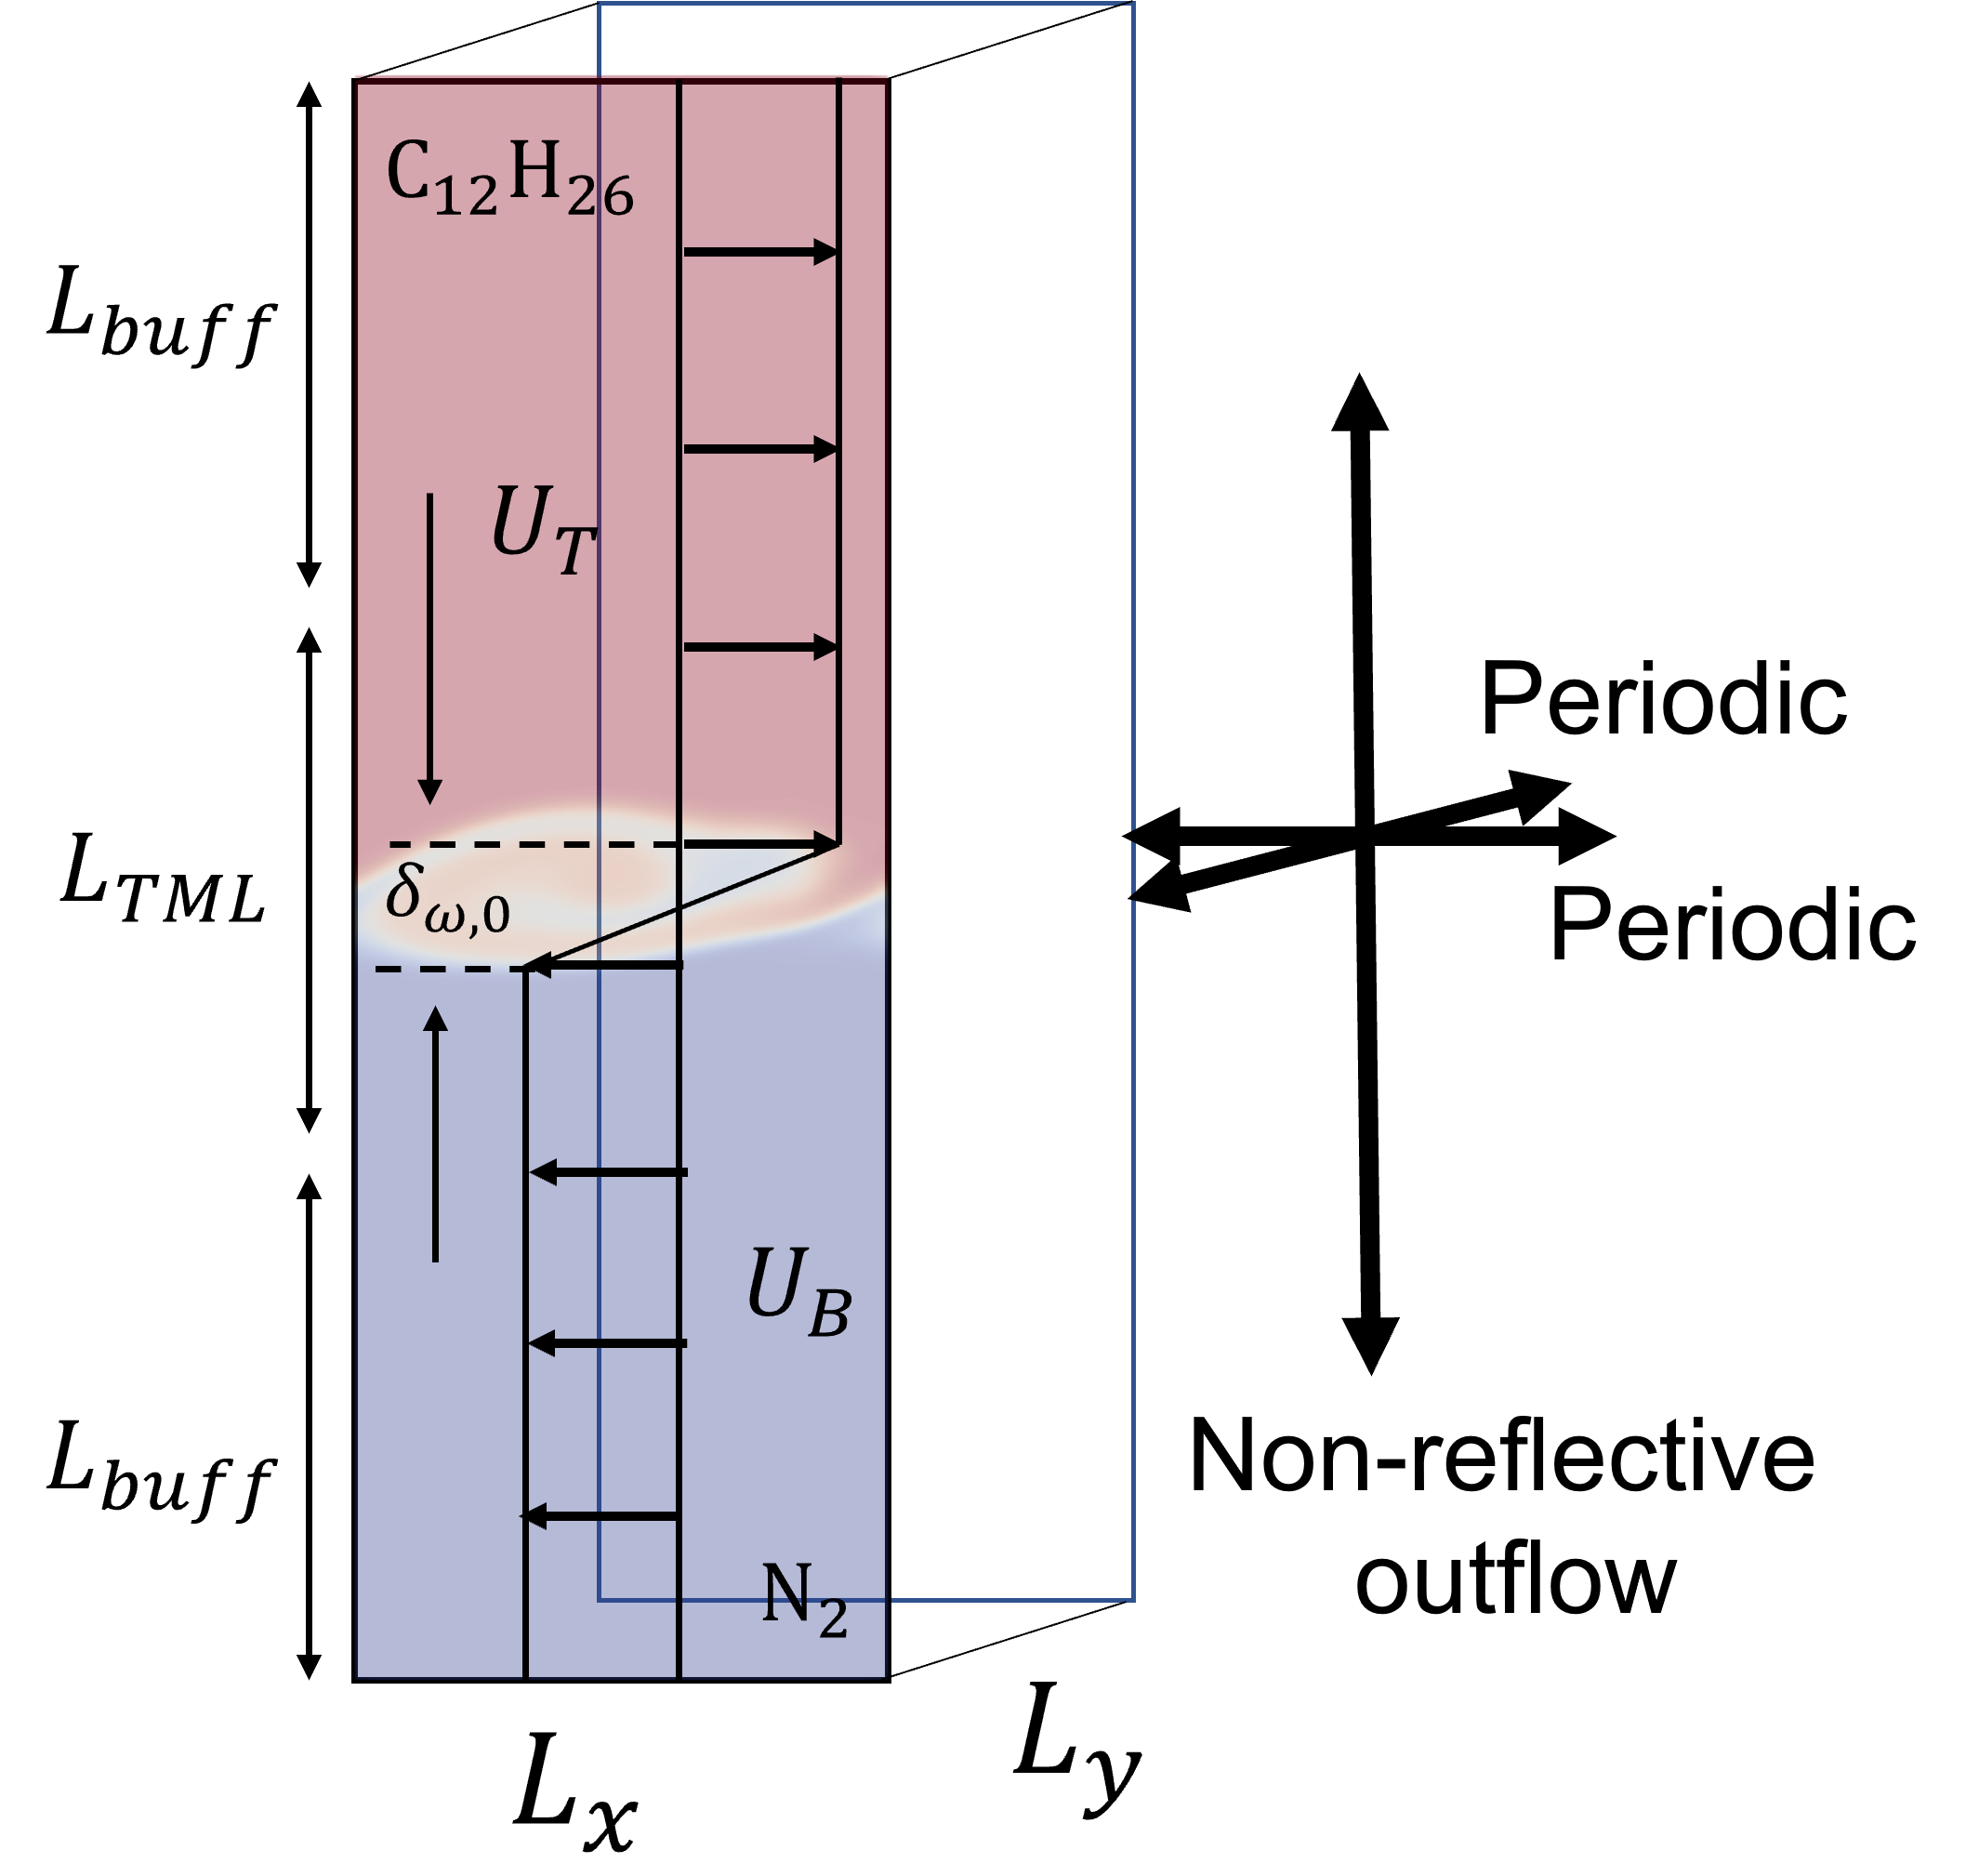
\includegraphics[width=0.45\linewidth]{TML_sc.png}
\hspace{.2in}
\raisebox{0.1\height}{
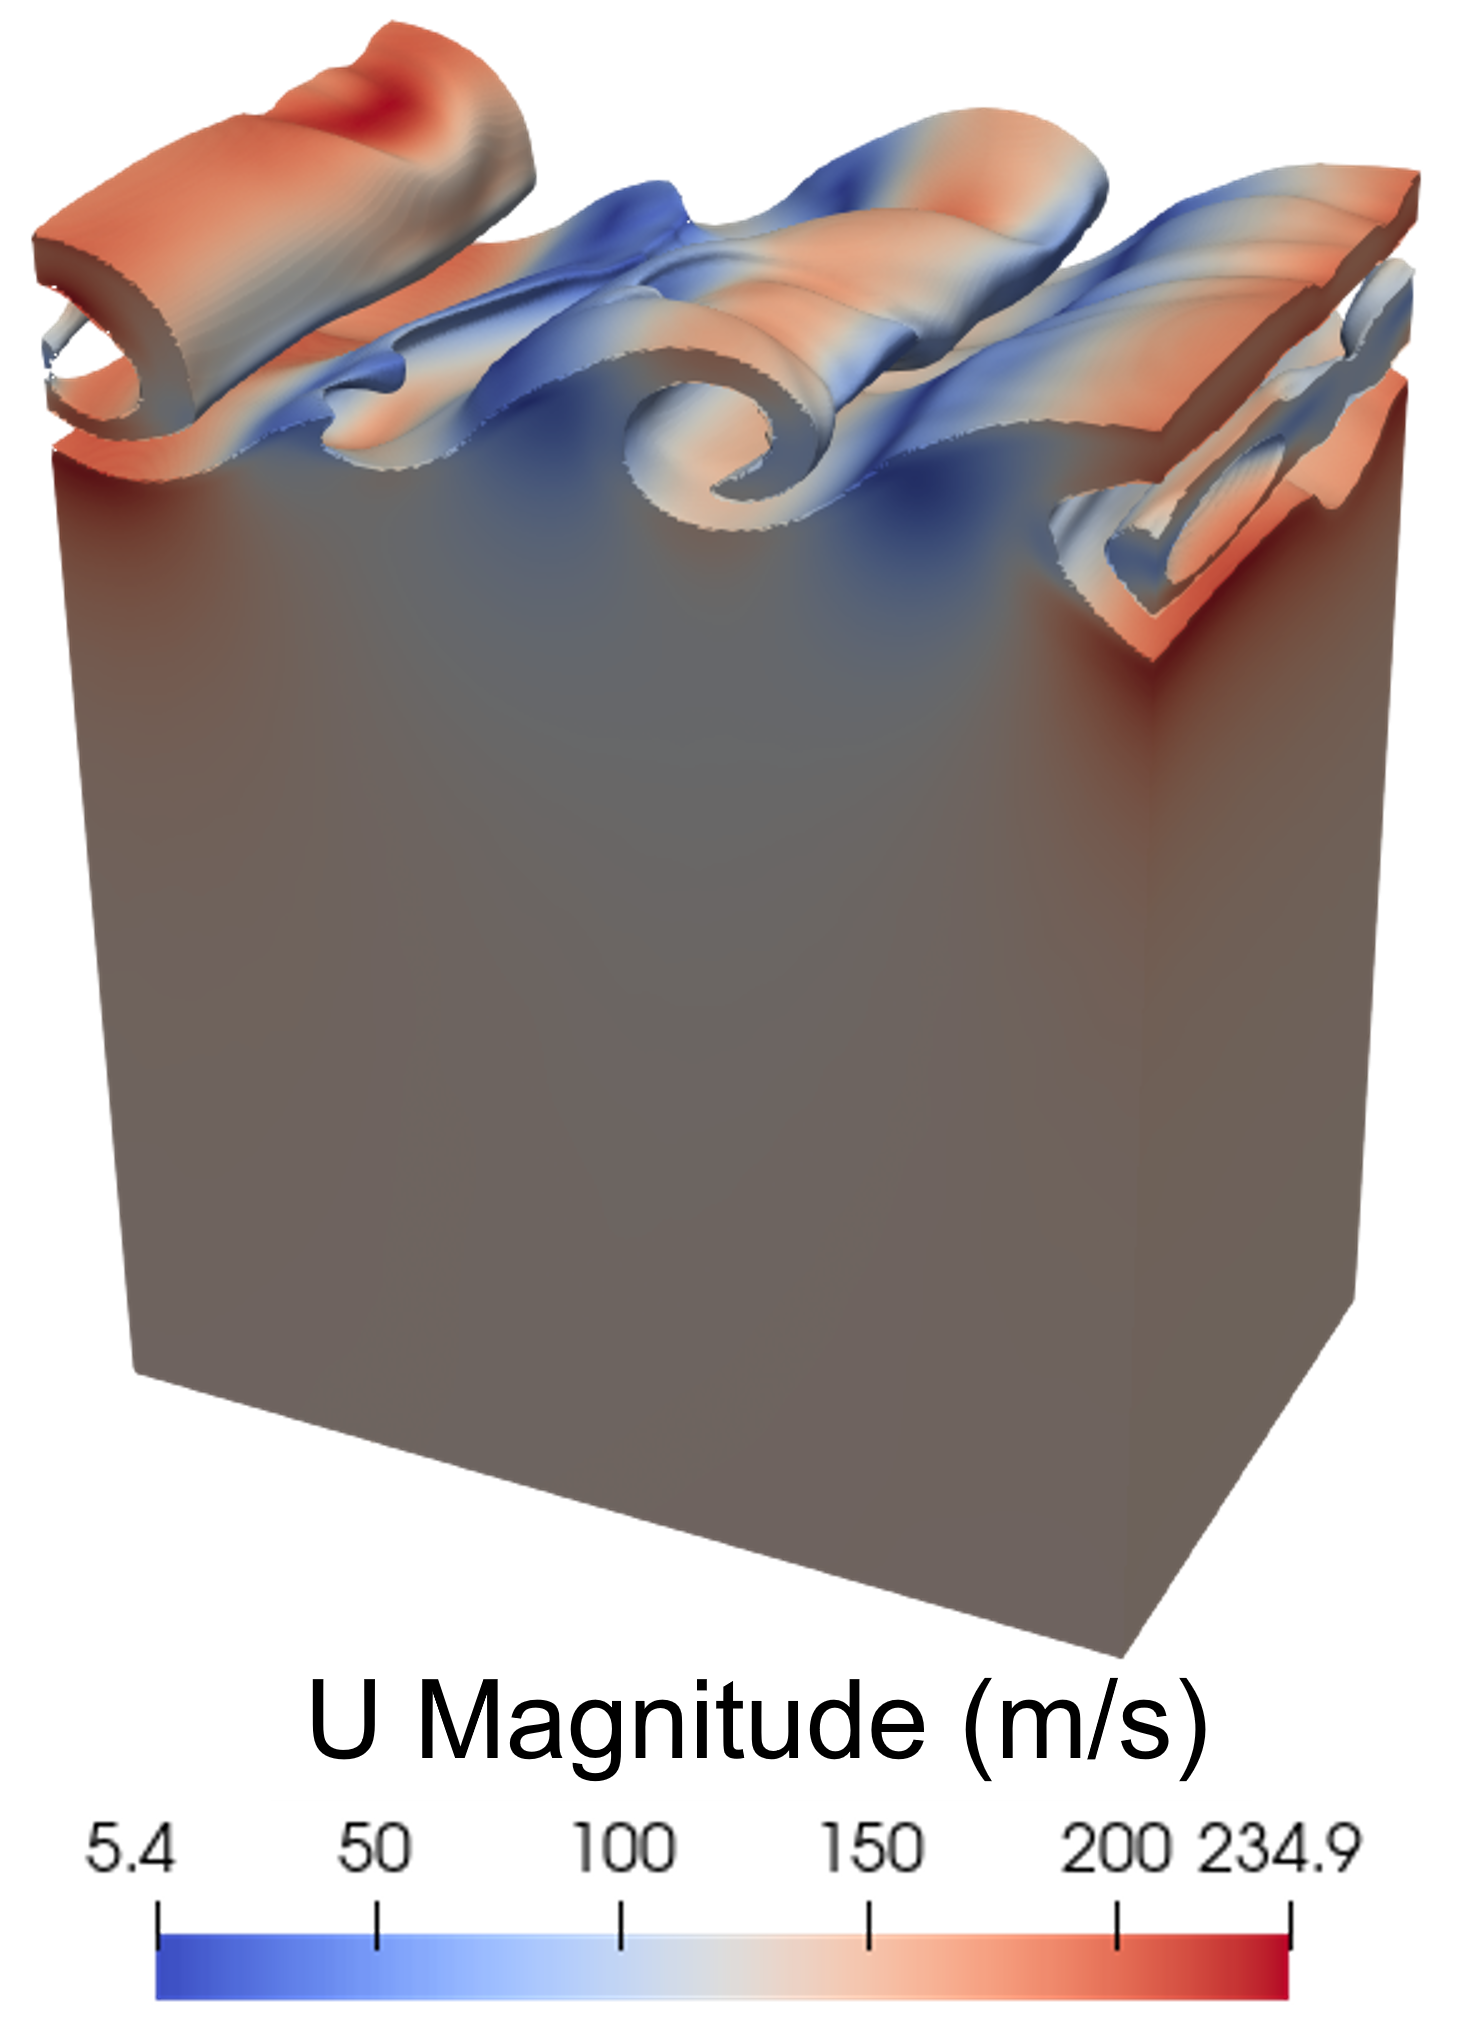
\includegraphics[width=0.25\linewidth]{3D_sc_s2.png}}
\caption{Left: Configuration of transcritical temporal mixing layer (TML) simulations. Right: 3D VLE-based CFD simulation of the transcritical TML, $t=2\times 10^-7s$, iso-surface: mass fraction of n-dodecane $Y_{C_{12}H_{26}} = 0.3$, color: velocity magnitude.}
\label{TML_GEO} 
\end{figure}


%\begin{table}%[width=0.9\linewidth,cols=4,pos=h]
%\caption{The initial condition of temporal mixing layer.}\label{TML_init_table}
%\begin{threeparttable} 
%\begin{tabular*}{\tblwidth}{@{} L|LLLLL@{} }
%\toprule
%Properties     & $U_T (m/s)$   & $U_B (m/s)$  & $T_T (K)$   & $L_x (m)$ & $\delta_{\omega_0}$\\
%\midrule
%Case 1         & 77.94         & 134.27       & 600         & $2.79 \times 10^{-5}$   & $9.58 \times 10^{-7}$   \\
%Case 2         & 59.67         & 89.01        & 800         & $3.55 \times 10^{-5}$   & $1.22\times 10^{-6}$    \\
%\bottomrule
%\end{tabular*}
%         \begin{tablenotes}
%        \footnotesize    
%        \item Subscripts T and B refer to Top and Bottom, respectively. $L_y = 0.6\times L_x$,  $Re_0=1000$. Mesh in the center subdomain is $256\times 152 \times 256$, and the top and bottom subdomain mesh is $256\times 152\times 64$. $P = 50$ bar, $T_B=293$ K, $M_c = 0.3$, $A_i = 0.25, 0.5, 1$, $B_i = 0.05, 0, 1$, and $F_{2D}= F_{3D} = 0.05$.\\
       
%      \end{tablenotes}
%      \end{threeparttable}
%\end{table}

\begin{table}
    \caption{The initial condition of temporal mixing layer.}\label{TML_init_table}
    \begin{threeparttable} 
\begin{tabular*}{0.8\textwidth}{@{} l|lllll@{}}
    \toprule
    Properties     & $U_T (m/s)$   & $U_B (m/s)$  & $T_T (K)$   & $L_x (m)$ & $\delta_{\omega_0}$\\
    \midrule
    Case 1         & 77.94         & 134.27       & 600         & $2.79 \times 10^{-5}$   & $9.58 \times 10^{-7}$   \\
    Case 2         & 59.67         & 89.01        & 800         & $3.55 \times 10^{-5}$   & $1.22\times 10^{-6}$    \\
    \bottomrule
\end{tabular*}
\begin{tablenotes}
    \footnotesize    
    \item Subscripts T and B refer to Top and Bottom, respectively. $L_y = 0.6\times L_x$,  $Re_0=1000$. Mesh in the center subdomain is $256\times 152 \times 256$, and the top and bottom subdomain mesh is $256\times 152\times 64$. $P = 50$ bar, $T_B=293$ K, $M_c = 0.3$, $A_i = 0.25, 0.5, 1$, $B_i = 0.05, 0, 1$, and $F_{2D}= F_{3D} = 0.05$.\\
  \end{tablenotes}
\end{threeparttable}
\end{table}



\subsubsection{ISAT-VLE's performance and error control in 2D simulations:}





%First, 2D simulations are conducted to test ISAT performance and error control. 
In this subsection, we utilize the configuration of Case 1 in Table.~\ref{TML_init_table}. For 2D simulation, and the velocity in the y direction is set to zero. A set of error tolerance values are employed to assess the performance.  Using the FC method, the ISAT-VLE approach provides pressure, temperature, vapor fraction, and speed of sound results. The parameter $k$ is utilized to adjust the error tolerance, where the error tolerance $(T_{tol},p_{tol},\beta_{tol},c_{tol})= k (10^2, 10^6, 1, 10^2)$. This error tolerance is defined based on the magnitude of the properties, hence $k$ can be roughly considered as a maximum relative error. in which the order of magnitude of the tolerances depends on the magnitude of the properties. Hence, $k$ can be roughly considered as a maximum relative error. The simulation is run to $2\times 10^{-7}$ s to capture the vortex formation process from a flat interface under the influence of initial perturbation. 

Fig.~\ref{TML_PE}(a) illustrates the performance of the ISAT-VLE method. The blue dotted line represents the CPU time consumed by all other models in the CFD solver, which is significantly lower than the time consumed by the VLE model. Without the ISAT method, the VLE model accounts for 92.9\% of the CPU resources.The other curves in Fig.~\ref{TML_PE}(a) depict the accelerated performance of the VLE model with ISAT for different $k$ values (error tolerances), where a larger tolerance yields better performance. At the initial stage, the ISAT-VLE model runs approximately 15-61 times faster than the original VLE model, and in the final stage, it achieves a speed-up factor of 4-24. This is because the CPU time for all ISAT-VLE results increases as the mixing process generates more thermodynamic states. The performance curves of the ISAT-VLE results exhibit oscillation, which is attributed to the re-balancing of the binary tree when the overall structure becomes highly unbalanced (Sec.~\ref{sec:ISAT}). Simulations with larger tolerances exhibit shorter CPU times in each step, making the influence of re-balancing on performance (oscillation) more pronounced.


Fig.~\ref{TML_PE}(b) showcases the error control of the ISAT-VLE method. The errors presented in the plot are from the simulation with $k= 3 \times 10^{-3}$. The error is normalized by the tolerance, and the dashed line indicates that the error is equal to the tolerance ($\text{normalized error}=1$). The average error is evaluated using $\frac{\sum_i |e_i|V_i}{\sum_i V_i}$, where $V_i$ is cell volume, $e_i$ error in cell $i$. The average error is controlled to be 2 to 3 orders of magnitude smaller than the tolerance. Although the maximum error can exceed the tolerance, it remains within a similar order of magnitude. Table~\ref{TML_FC_table} shows the absolute and relative errors for all cases. As the tolerance decreases, the error is better controlled. For this particular simulation, $k= 3 \times 10^{-3}$ proves to be a suitable choice, ensuring pressure and temperature errors are kept within 0.5\% while achieving a total speed-up factor of 8.5.



\begin{figure}[htbp]
\centering
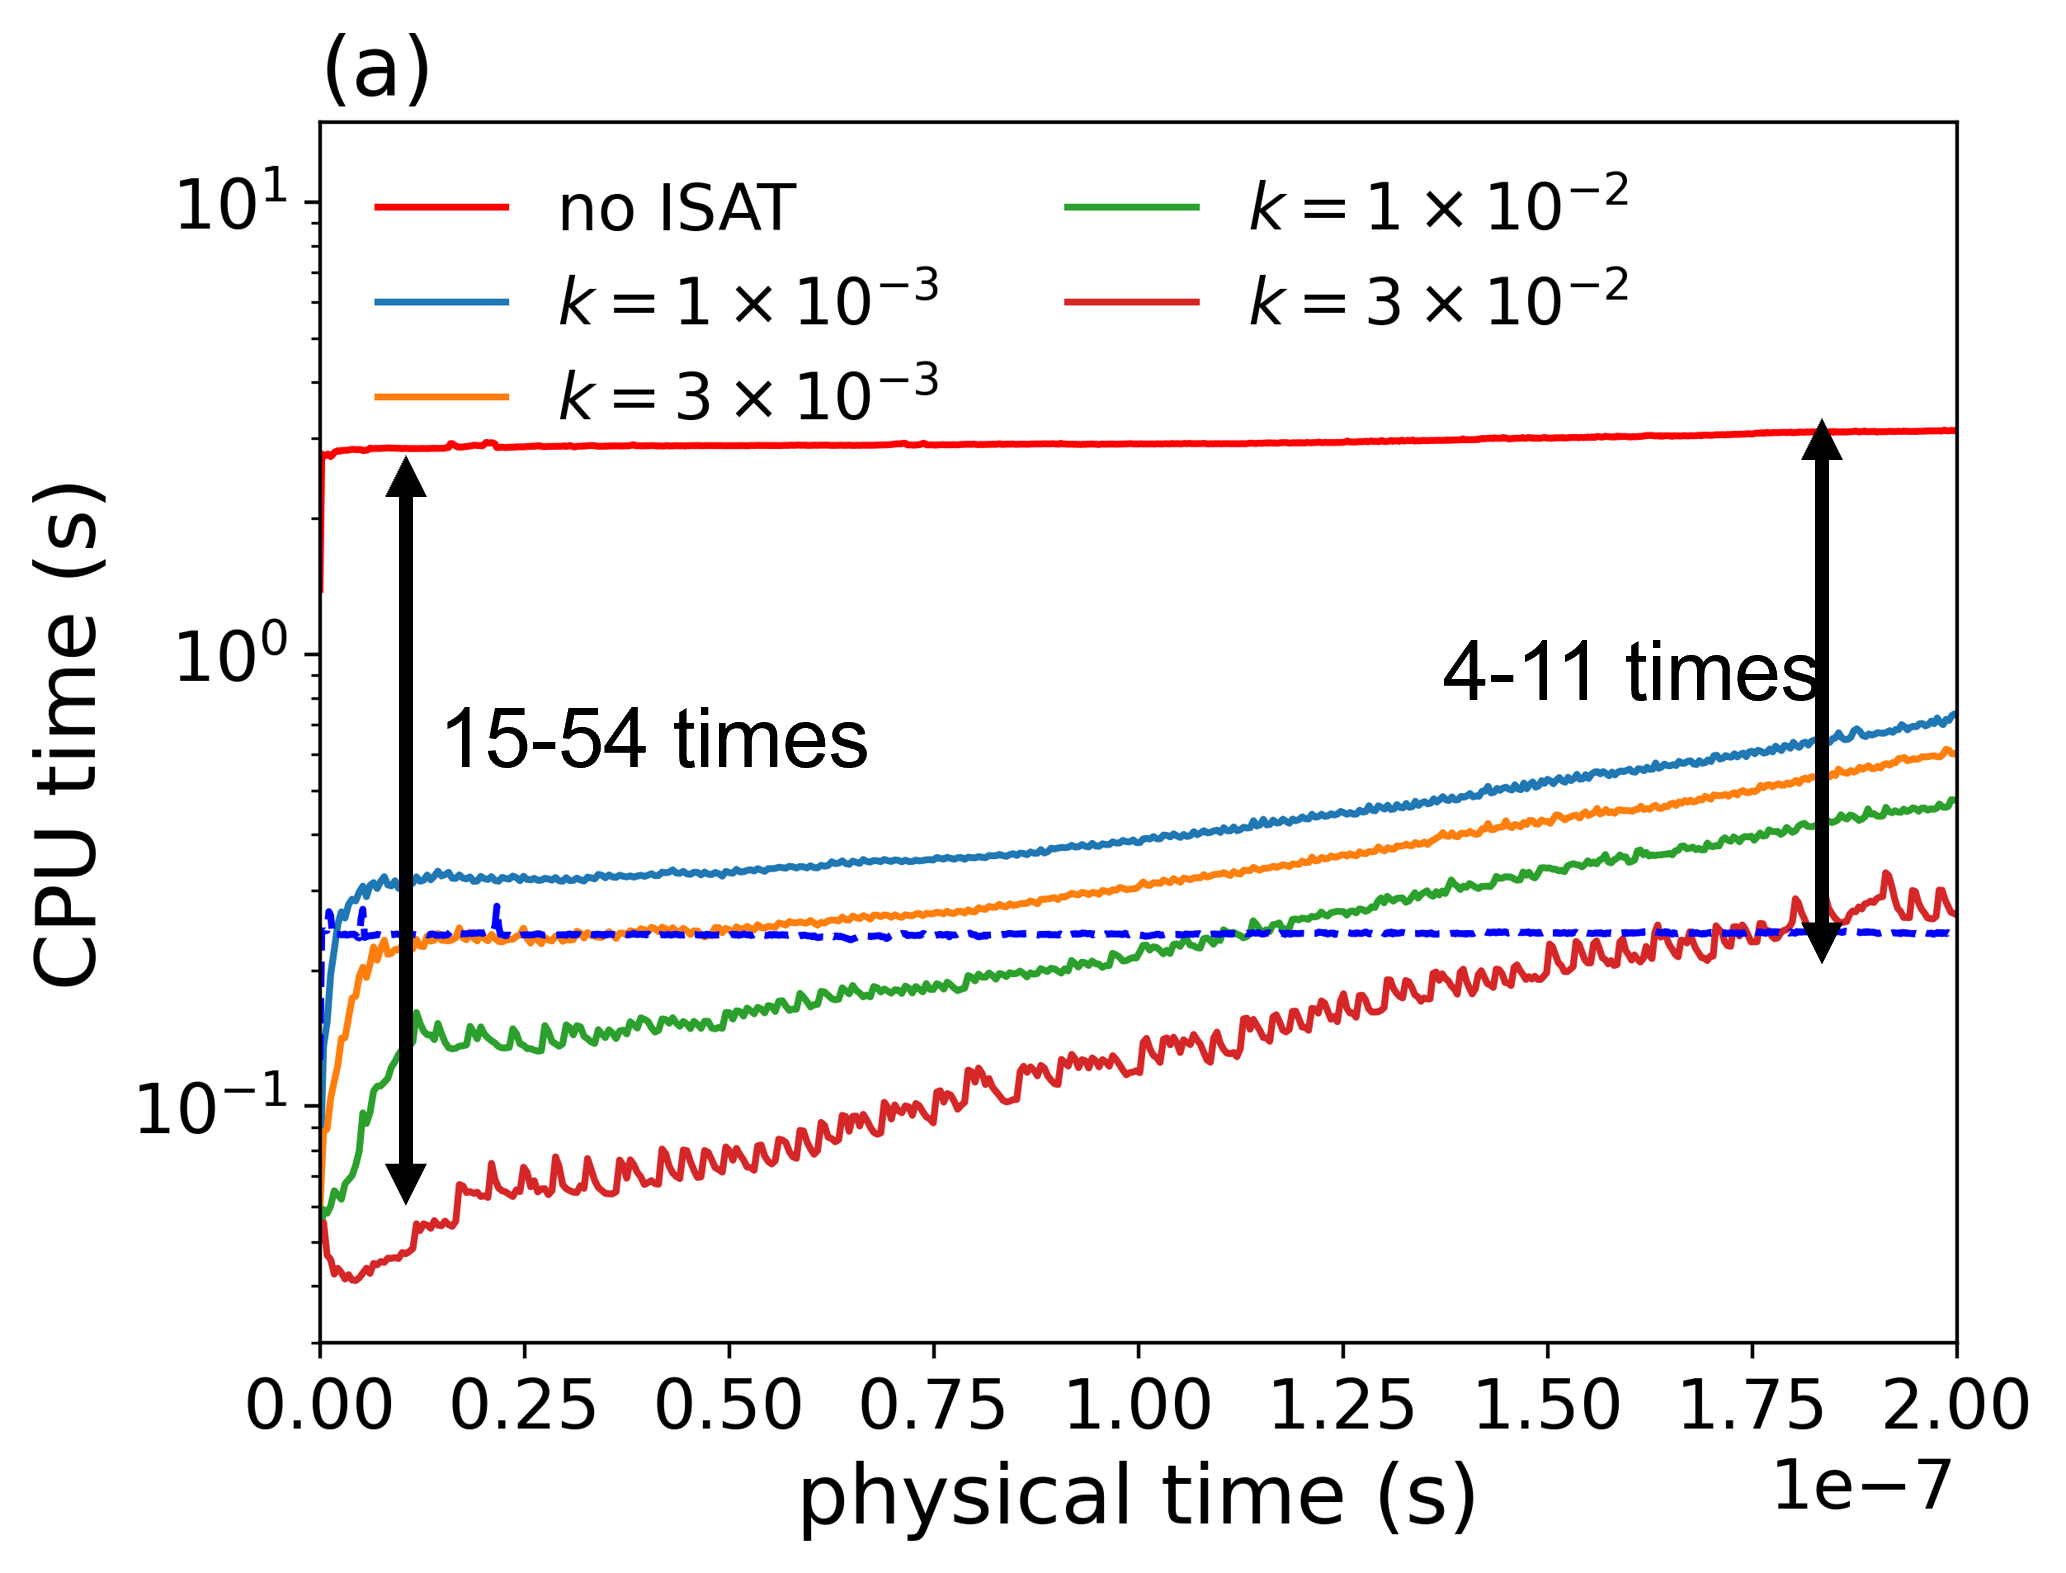
\includegraphics[width=0.45\linewidth]{time_TML_2D_m_2.png}
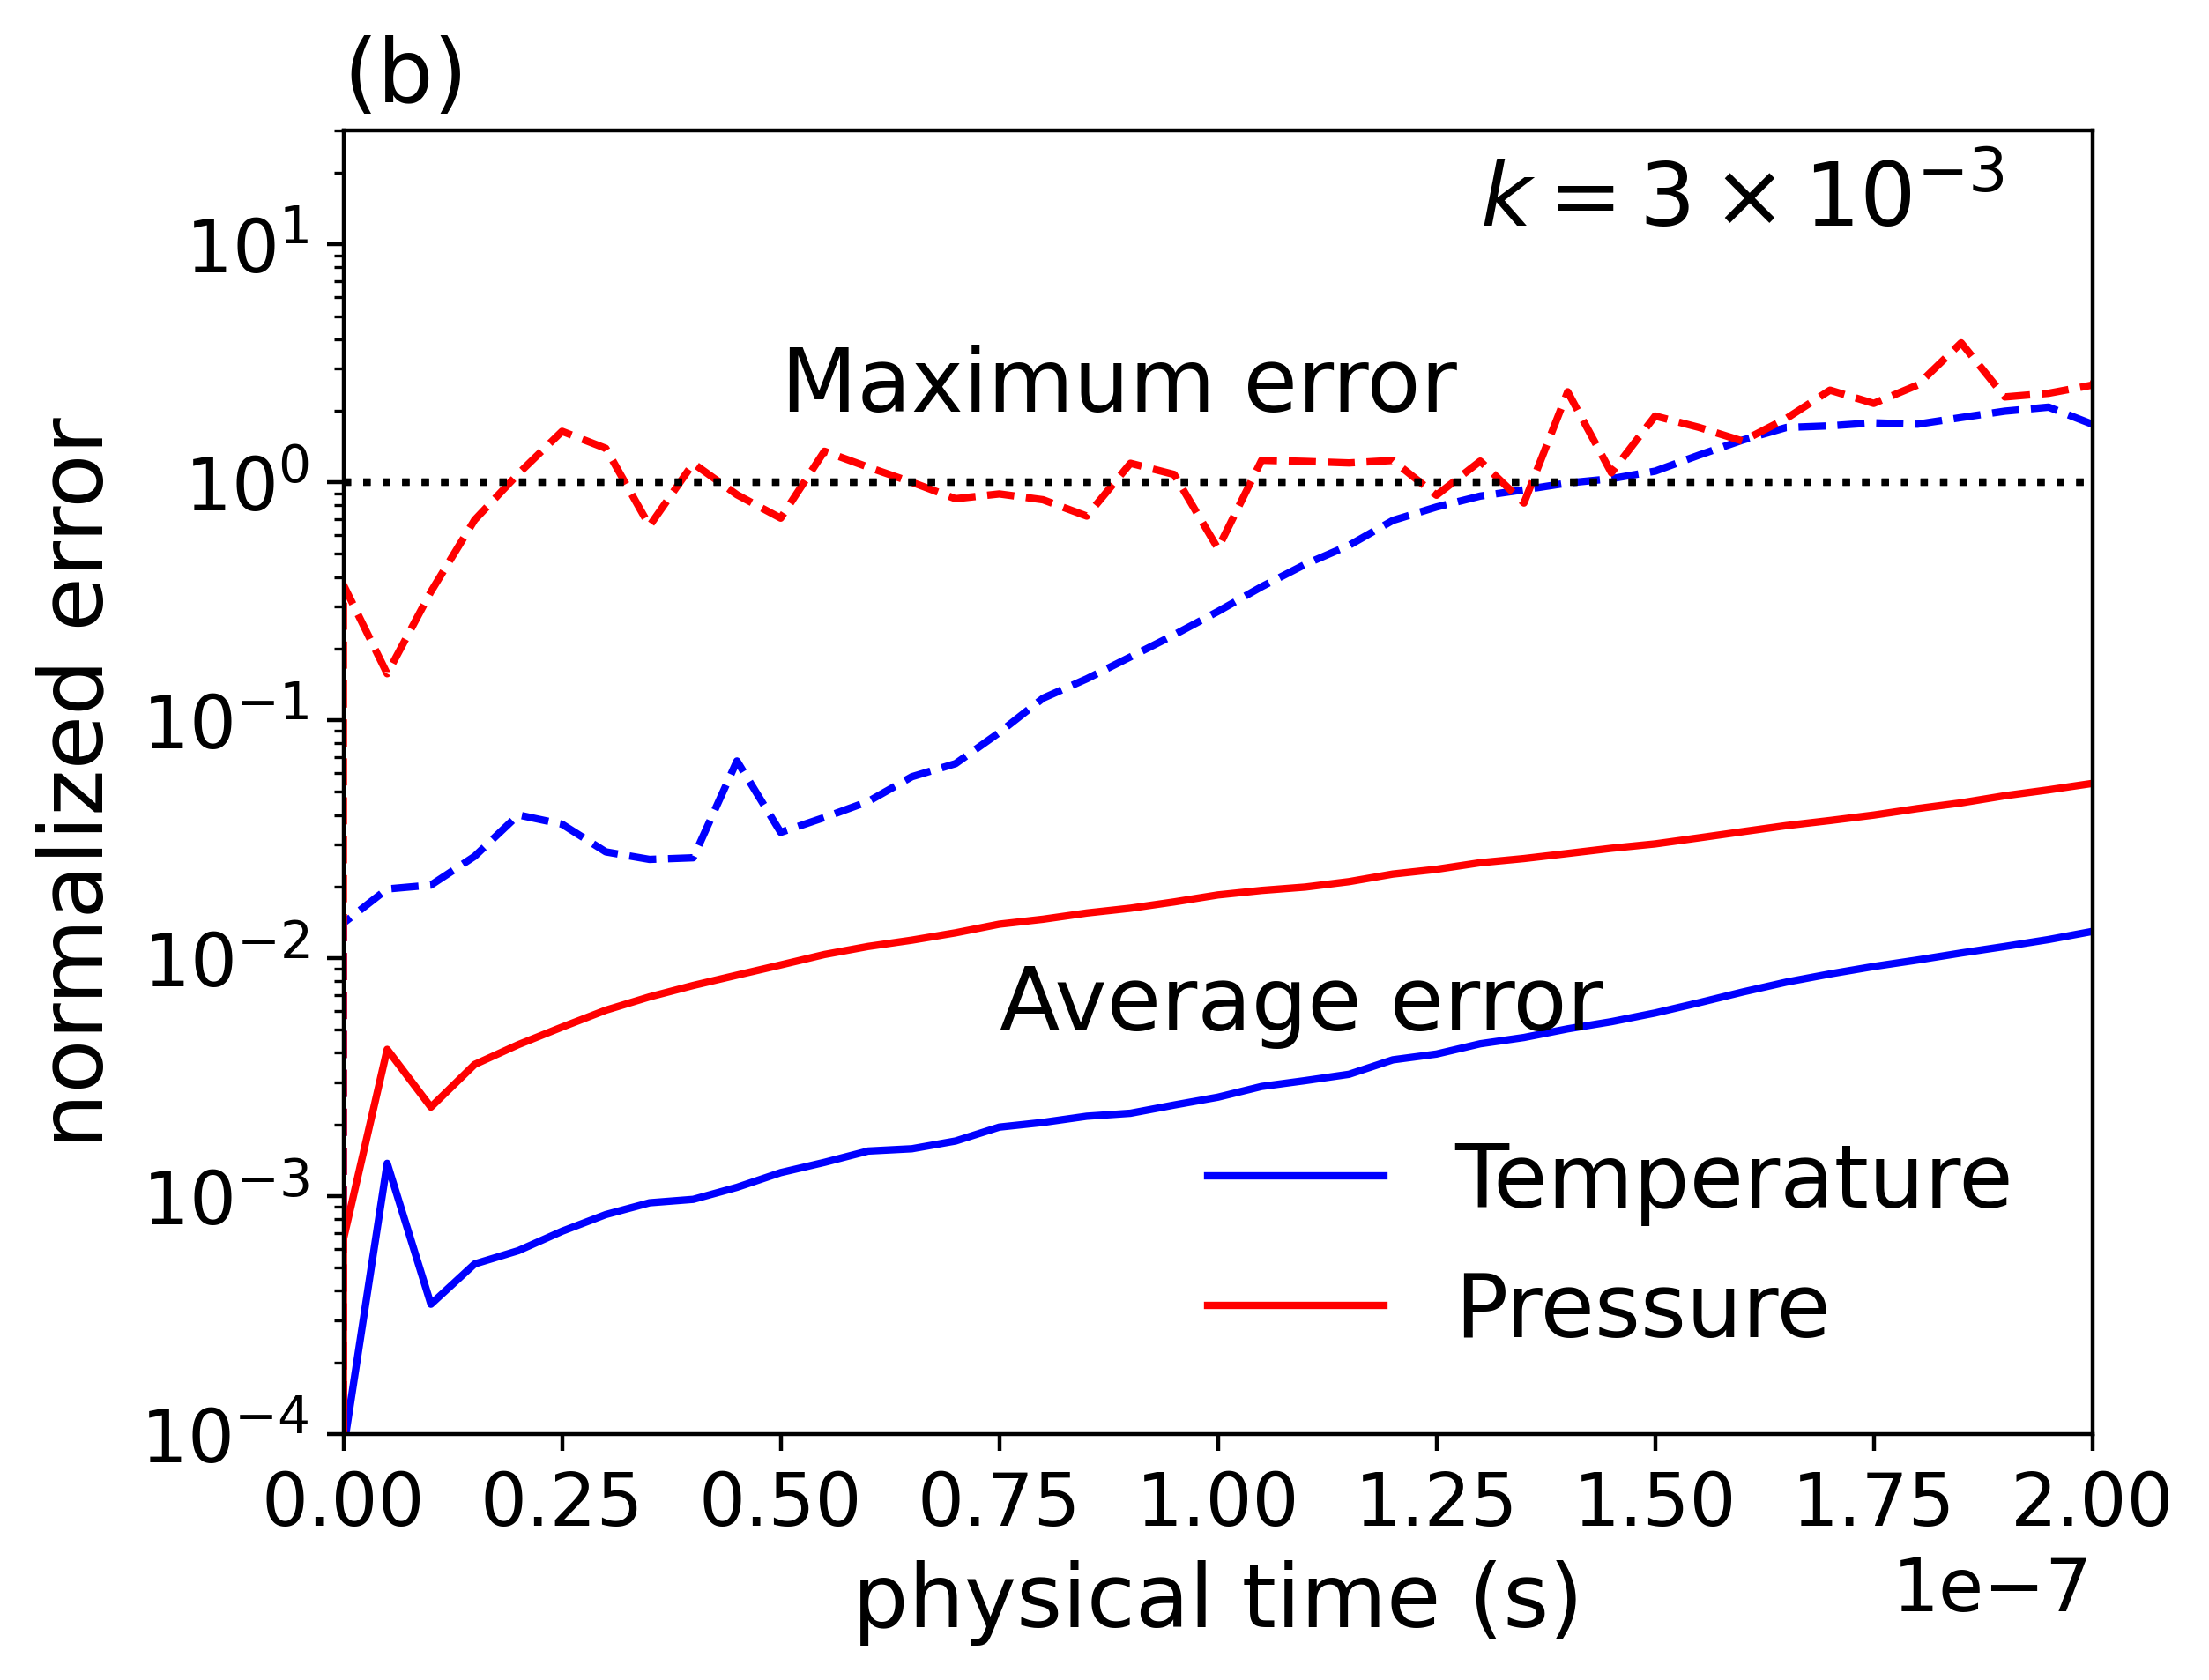
\includegraphics[width=0.45\linewidth]{error_TML_2D_3e_3_3.png}
\caption{(a) The performance of ISAT-VLE, in terms of the CPU time spent in every time step. The Blue dotted line is the CPU time of all other parts of the CFD solver, except the VLE model; the top red line is the CPU time of the VLE model without ISAT. In addition, 4 lines of the ISAT-VLE model with different tolerances ($k$) are provided. (b) The error control of ISAT-VLE, in terms of the normalized average error and maximum error versus physical time, $k=3\times 10^{-3}$.}
\label{TML_PE} 
\end{figure}



%\begin{table}[width=.9\linewidth,cols=4,pos=h]
%\caption{The performance and errors of ISAT-VLE in TML cases with different error tolerance.}\label{TML_FC_table}
%\begin{tabular*}{\tblwidth}{@{} L|LLLLL@{} }
%\toprule
%$k$                   & $1\times 10^{-3}$   & $3\times 10^{-3}$    & $1\times 10^{-2}$    &$3\times 10^{-2}$  \\%  & $1\times 10^{-1}$ \\
%\midrule
%Speed-up            & 6.7                  & 8.5                  & 11.6                 & 19.9                \\%  &  41.6          \\
%$P$ mean error (bar) & $8.2\times 10^{-4}$  & $1.5\times 10^{-3}$  & $0.7\times 10^{-3}$  & $1.6\times 10^{-2}$\\%  & $2.8\times 10^{-1}$ \\
%$P$ max error (bar)  & 0.06                 & 0.07                & 0.27                 & 1.0               \\% & 2.1              \\
%$P$ max relative error (\%) &0.16                 & 0.20                & 0.71                 & 2.8           \\%     & 5.1              \\
%$T$ mean error (K)   & $1.6\times 10^{-3}$  & $3.5\times 10^{-3}$  & $1.4\times 10^{-3}$  & $4\times 10^{-2}$ \\% & $7\times 10^{-1}$ \\
%$T$ max error (K)    & 0.16                  & 0.6                  & 2.1                  & 6.4                \\%  &   60          \\
%$T$ max relative error (\%) &0.05                 & 0.21                 & 0.73                 & 2.1             \\%   & 18.7              \\%
%\bottomrule
%\end{tabular*}
%\end{table}

\begin{table}%[width=.9\linewidth,cols=4,pos=h]
\caption{The performance and errors of ISAT-VLE in TML cases with different error tolerance.}\label{TML_FC_table}
\begin{tabular*}{0.8\textwidth}{@{} l|lllll@{} }
\toprule
$k$                   & $1\times 10^{-3}$   & $3\times 10^{-3}$    & $1\times 10^{-2}$    &$3\times 10^{-2}$  \\%  & $1\times 10^{-1}$ \\
\midrule
Speed-up            & 6.7                  & 8.5                  & 11.6                 & 19.9                \\%  &  41.6          \\
$P$ mean error (bar) & $8.2\times 10^{-4}$  & $1.5\times 10^{-3}$  & $0.7\times 10^{-3}$  & $1.6\times 10^{-2}$\\%  & $2.8\times 10^{-1}$ \\
$P$ max error (bar)  & 0.06                 & 0.07                & 0.27                 & 1.0               \\% & 2.1              \\
$P$ max relative error (\%) &0.16                 & 0.20                & 0.71                 & 2.8           \\%     & 5.1              \\
$T$ mean error (K)   & $1.6\times 10^{-3}$  & $3.5\times 10^{-3}$  & $1.4\times 10^{-3}$  & $4\times 10^{-2}$ \\% & $7\times 10^{-1}$ \\
$T$ max error (K)    & 0.16                  & 0.6                  & 2.1                  & 6.4                \\%  &   60          \\
$T$ max relative error (\%) &0.05                 & 0.21                 & 0.73                 & 2.1             \\%   & 18.7              \\%
\bottomrule
\end{tabular*}
\end{table}

\subsubsection{3D TML ISAT simulations:}

As recommended in the preceding section, $k = 3\times 10^{-2}$ is used for the 3D TML simulation.
As suggested in the previous section, $k = 3\times 10^{-2}$ is used for the 3D TML simulations. Simulations of Case 1 and Case 2 are conducted with the configurations detailed in Table~\ref{TML_init_table}. A grid convergence study is conducted using the configuration of Case 1, shown in Appendix~\ref{App:TML}. The development of vortices is depicted in Fig.~\ref{TML_3D_evo}. At $t = 1\times 10^{-7}$, the introduction of velocity perturbation in the initial condition causes distortion of the interface. Due to the Kelvin-Helmholtz (K-H) instability, three vortices form on the interface at $1.5 \times 10^{-7}$. Within the vortex center, a low-pressure area is generated, and acoustic waves propagate outward continuously, which can be clearly seen in the pressure at $2\times 10^{-7}$. The quantity $\alpha=\beta(1-\beta)$ serves as an indicator of the two-phase interface. The $\alpha$ contours reveal that under these conditions, phase separation is highly pronounced at the interface between \ce{n-C12H26} and \ce{N2}.%, necessitating VLE modeling. 

\begin{figure}[htbp]
\centering
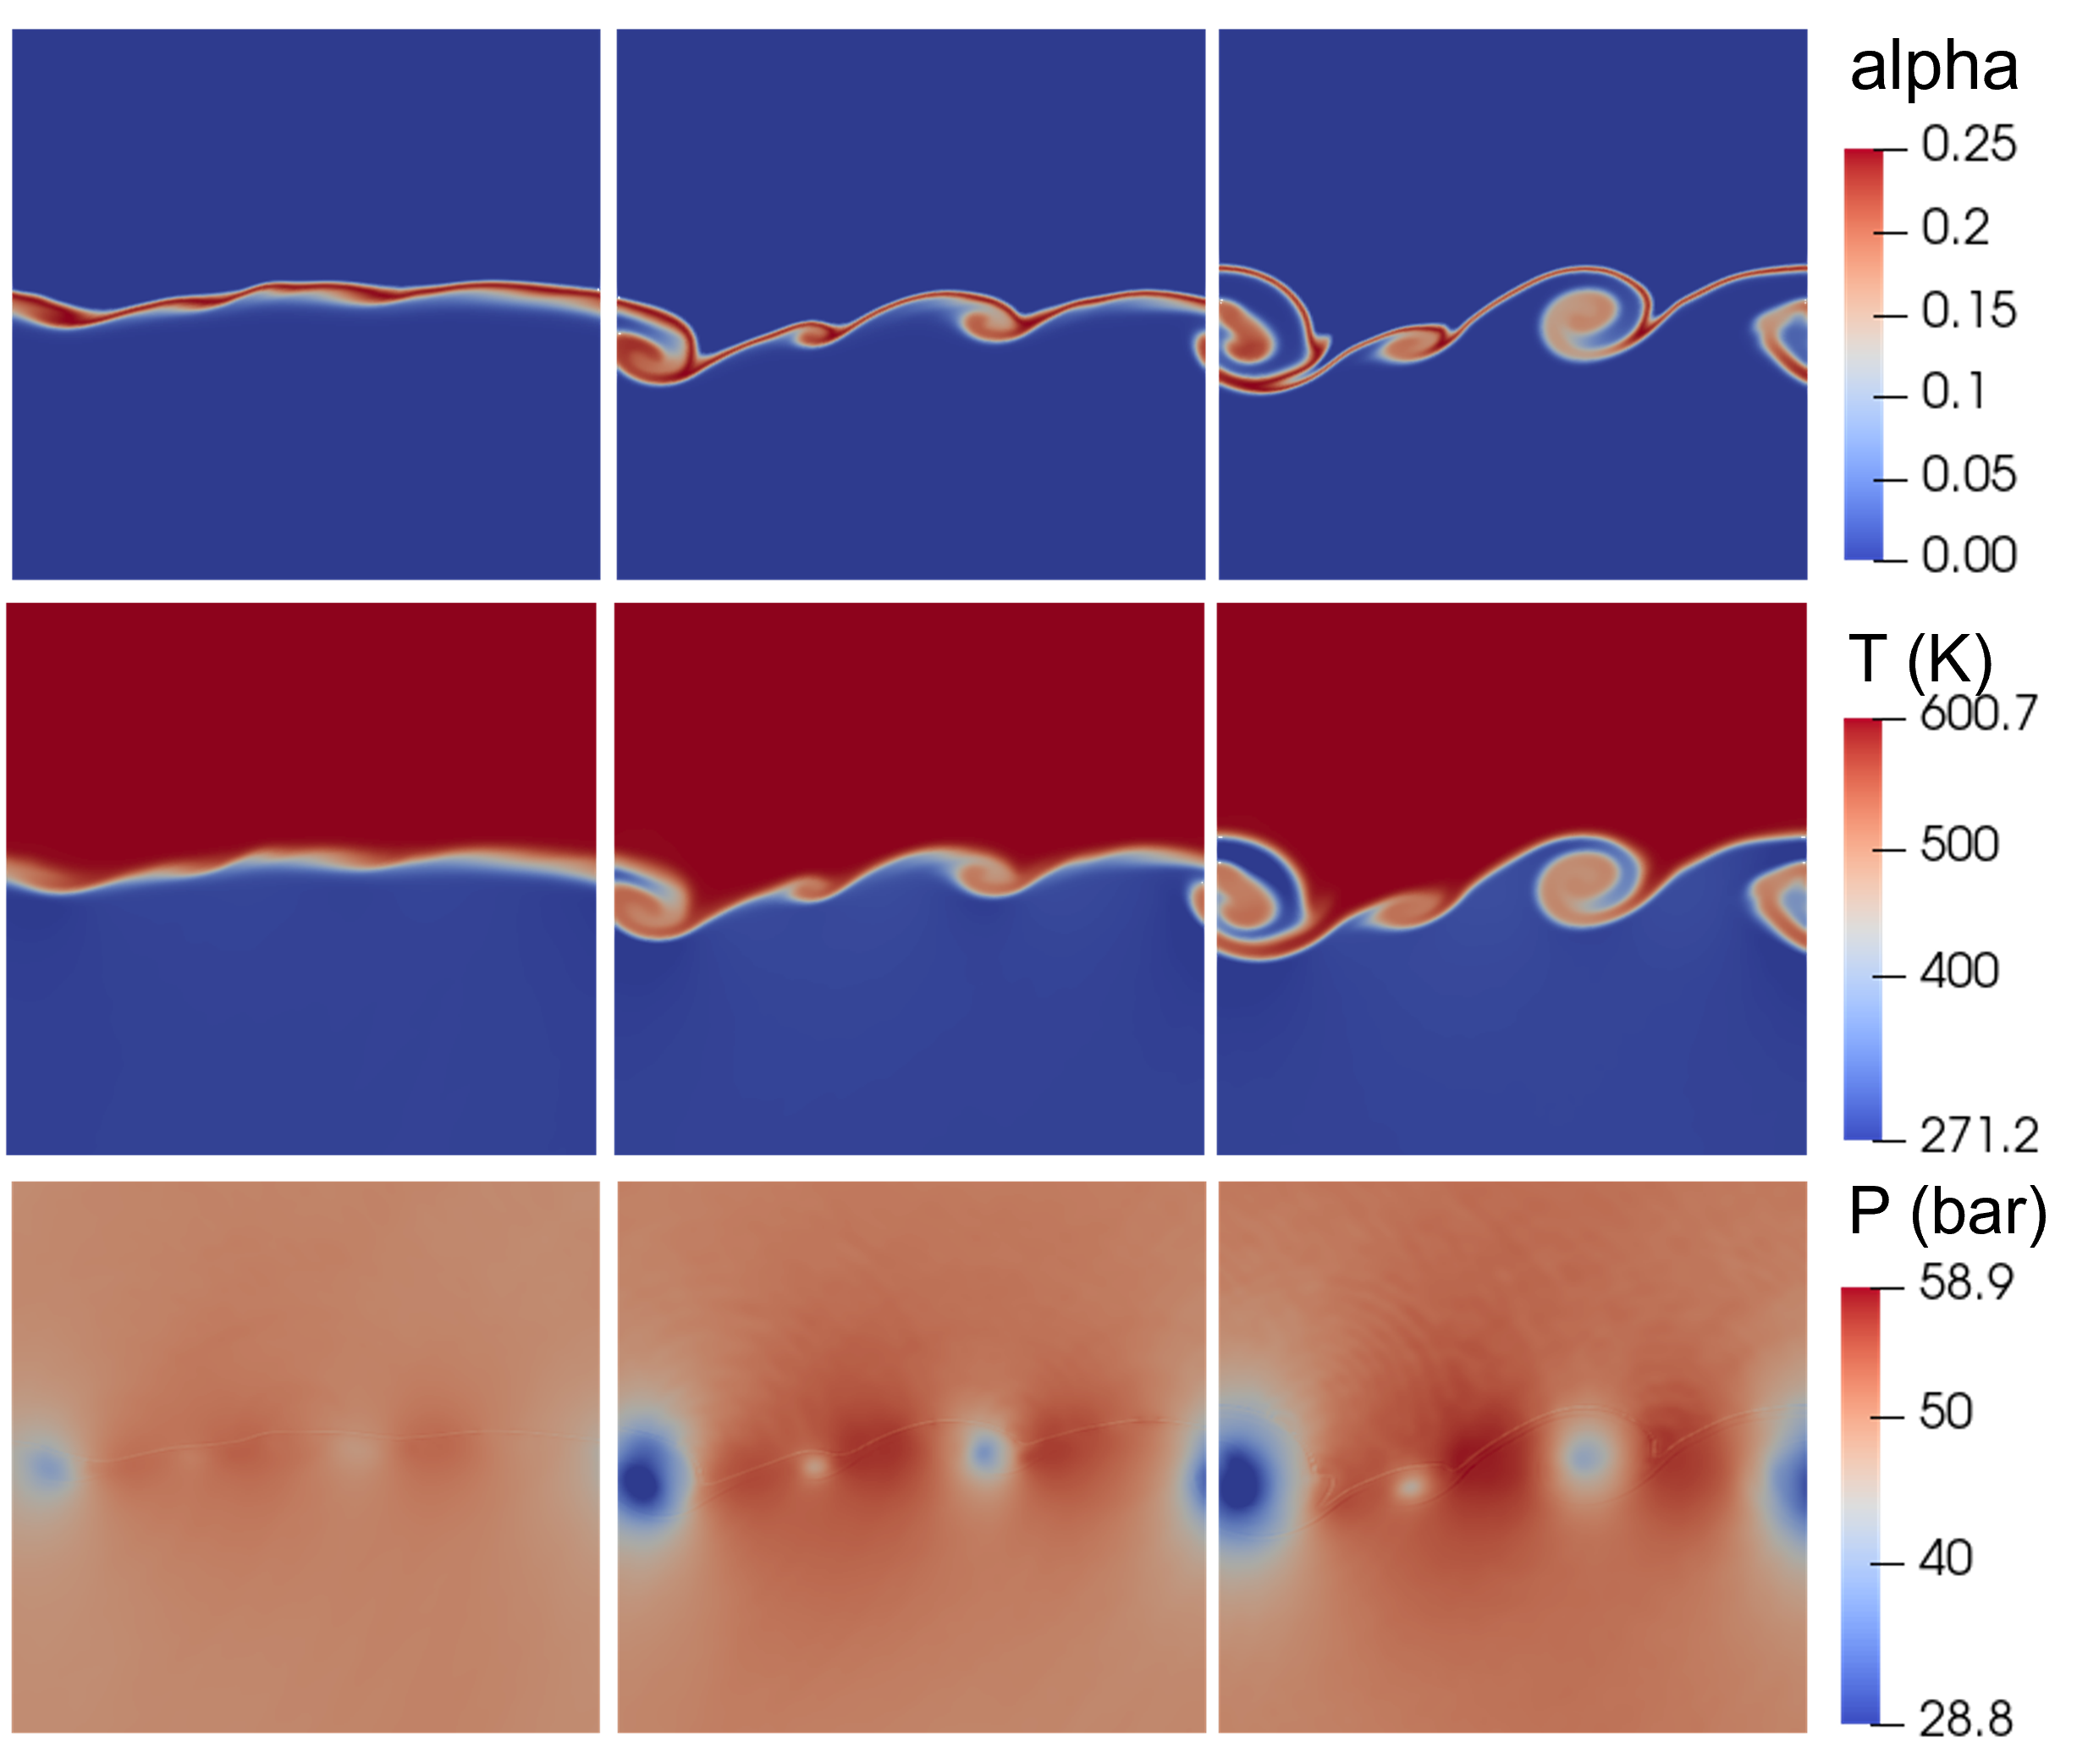
\includegraphics[width=0.65\linewidth]{TML_evo.png}
\caption{The vortex development in the 3D temporal mixing layer (TML): three snapshots at $t = 1\times 10^{-7}, 1.5 \times 10^{-7}, 2\times 10^{-7}$ s are shown in the figure.}
\label{TML_3D_evo} 
\end{figure}

Fig.~\ref{TML_3D_err} shows the temporal evolution of pressure and temperature errors. These values are obtained by calculating the absolute difference between the results obtained with the ISAT-VLE method and those obtained without it (e.g., $|T_{ISAT}-T_{noISAT}|$). As shown in Fig.~\ref{TML_3D_err}, both the temperature and pressure errors exhibit a gradual increase over time. However, the overall error remains at a very low level. The temperature deviation is primarily concentrated at the interface, with a maximum deviation of less than 5 K and a relative error of less than 1\%. The pressure error is more widespread due to the propagation of acoustic waves, but the majority of errors remain below 0.1 bar. The maximum error occurs at the interface and reaches approximately 0.2 bar. This error level is fully acceptable for the simulation, considering the average ambient pressure of around 50 bar, and the relative pressure error remains within 0.5\%.



\begin{figure}[htbp]
\centering
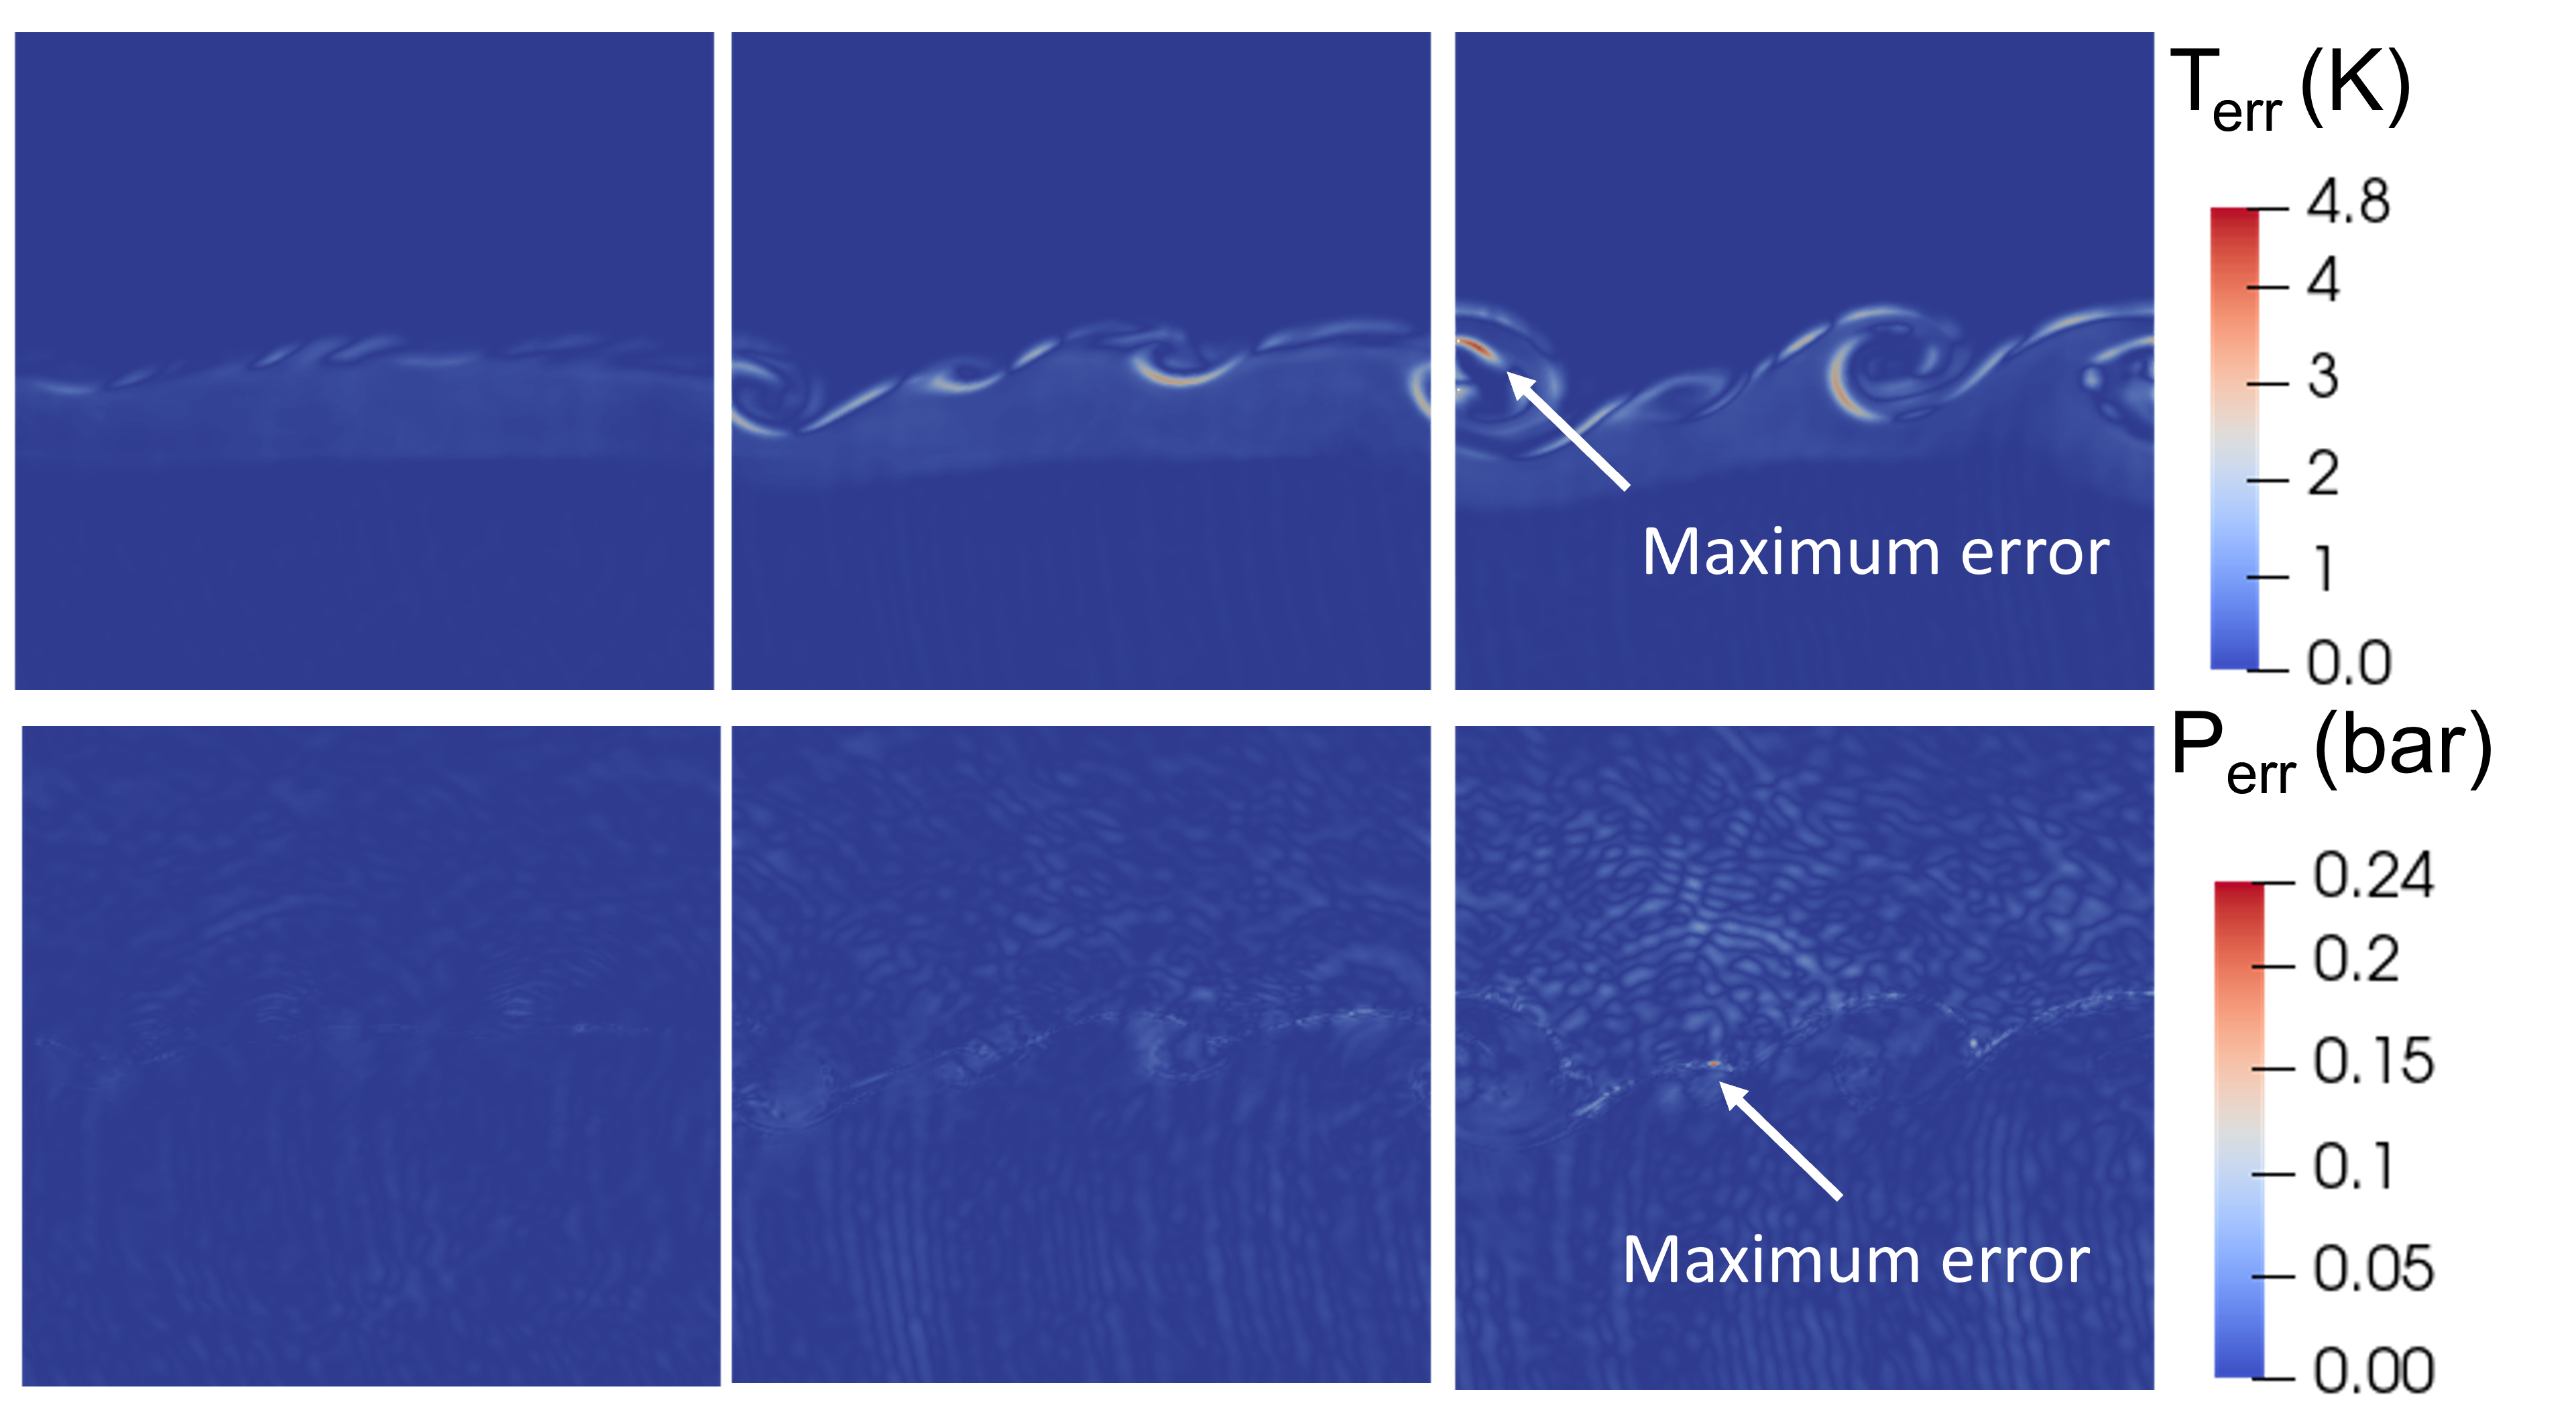
\includegraphics[width=0.65\linewidth]{TML_err.png}
\caption{The errors of the ISAT-VLE method in the 3D temporal mixing layer (TML): three snapshots at $t = 1\times 10^{-7}, 1.5 \times 10^{-7}, 2\times 10^{-7}$ s are shown in the figure.}
\label{TML_3D_err} 
\end{figure}


To compare the results of Case 1 and Case 2, a normalized time parameter $\tau = t \Delta U/ \delta_{\omega,0}$  is employed. Fig.~\ref{TML_3D_result} compares the results at $\tau = 45$, corresponding to the formation of the vortex. In both cases, a two-phase region is observed at the interface. However, in Case 2, the phase separation is significantly weaker despite the presence of cold \ce{N2} (293 K). This can be attributed to the high temperature of \ce{n-C12H26} (800 K), which hinders its cooling by the cold \ce{N2}.  As a result, even at the interface, the majority of mixtures remain in the gas phase. However, in the vicinity of the vortex, where mixing is more pronounced, a slightly stronger phase separation is observed. The crucial role of the VLE model becomes apparent in capturing these differences in phase separation under different conditions.


\begin{figure}[htbp]
\centering
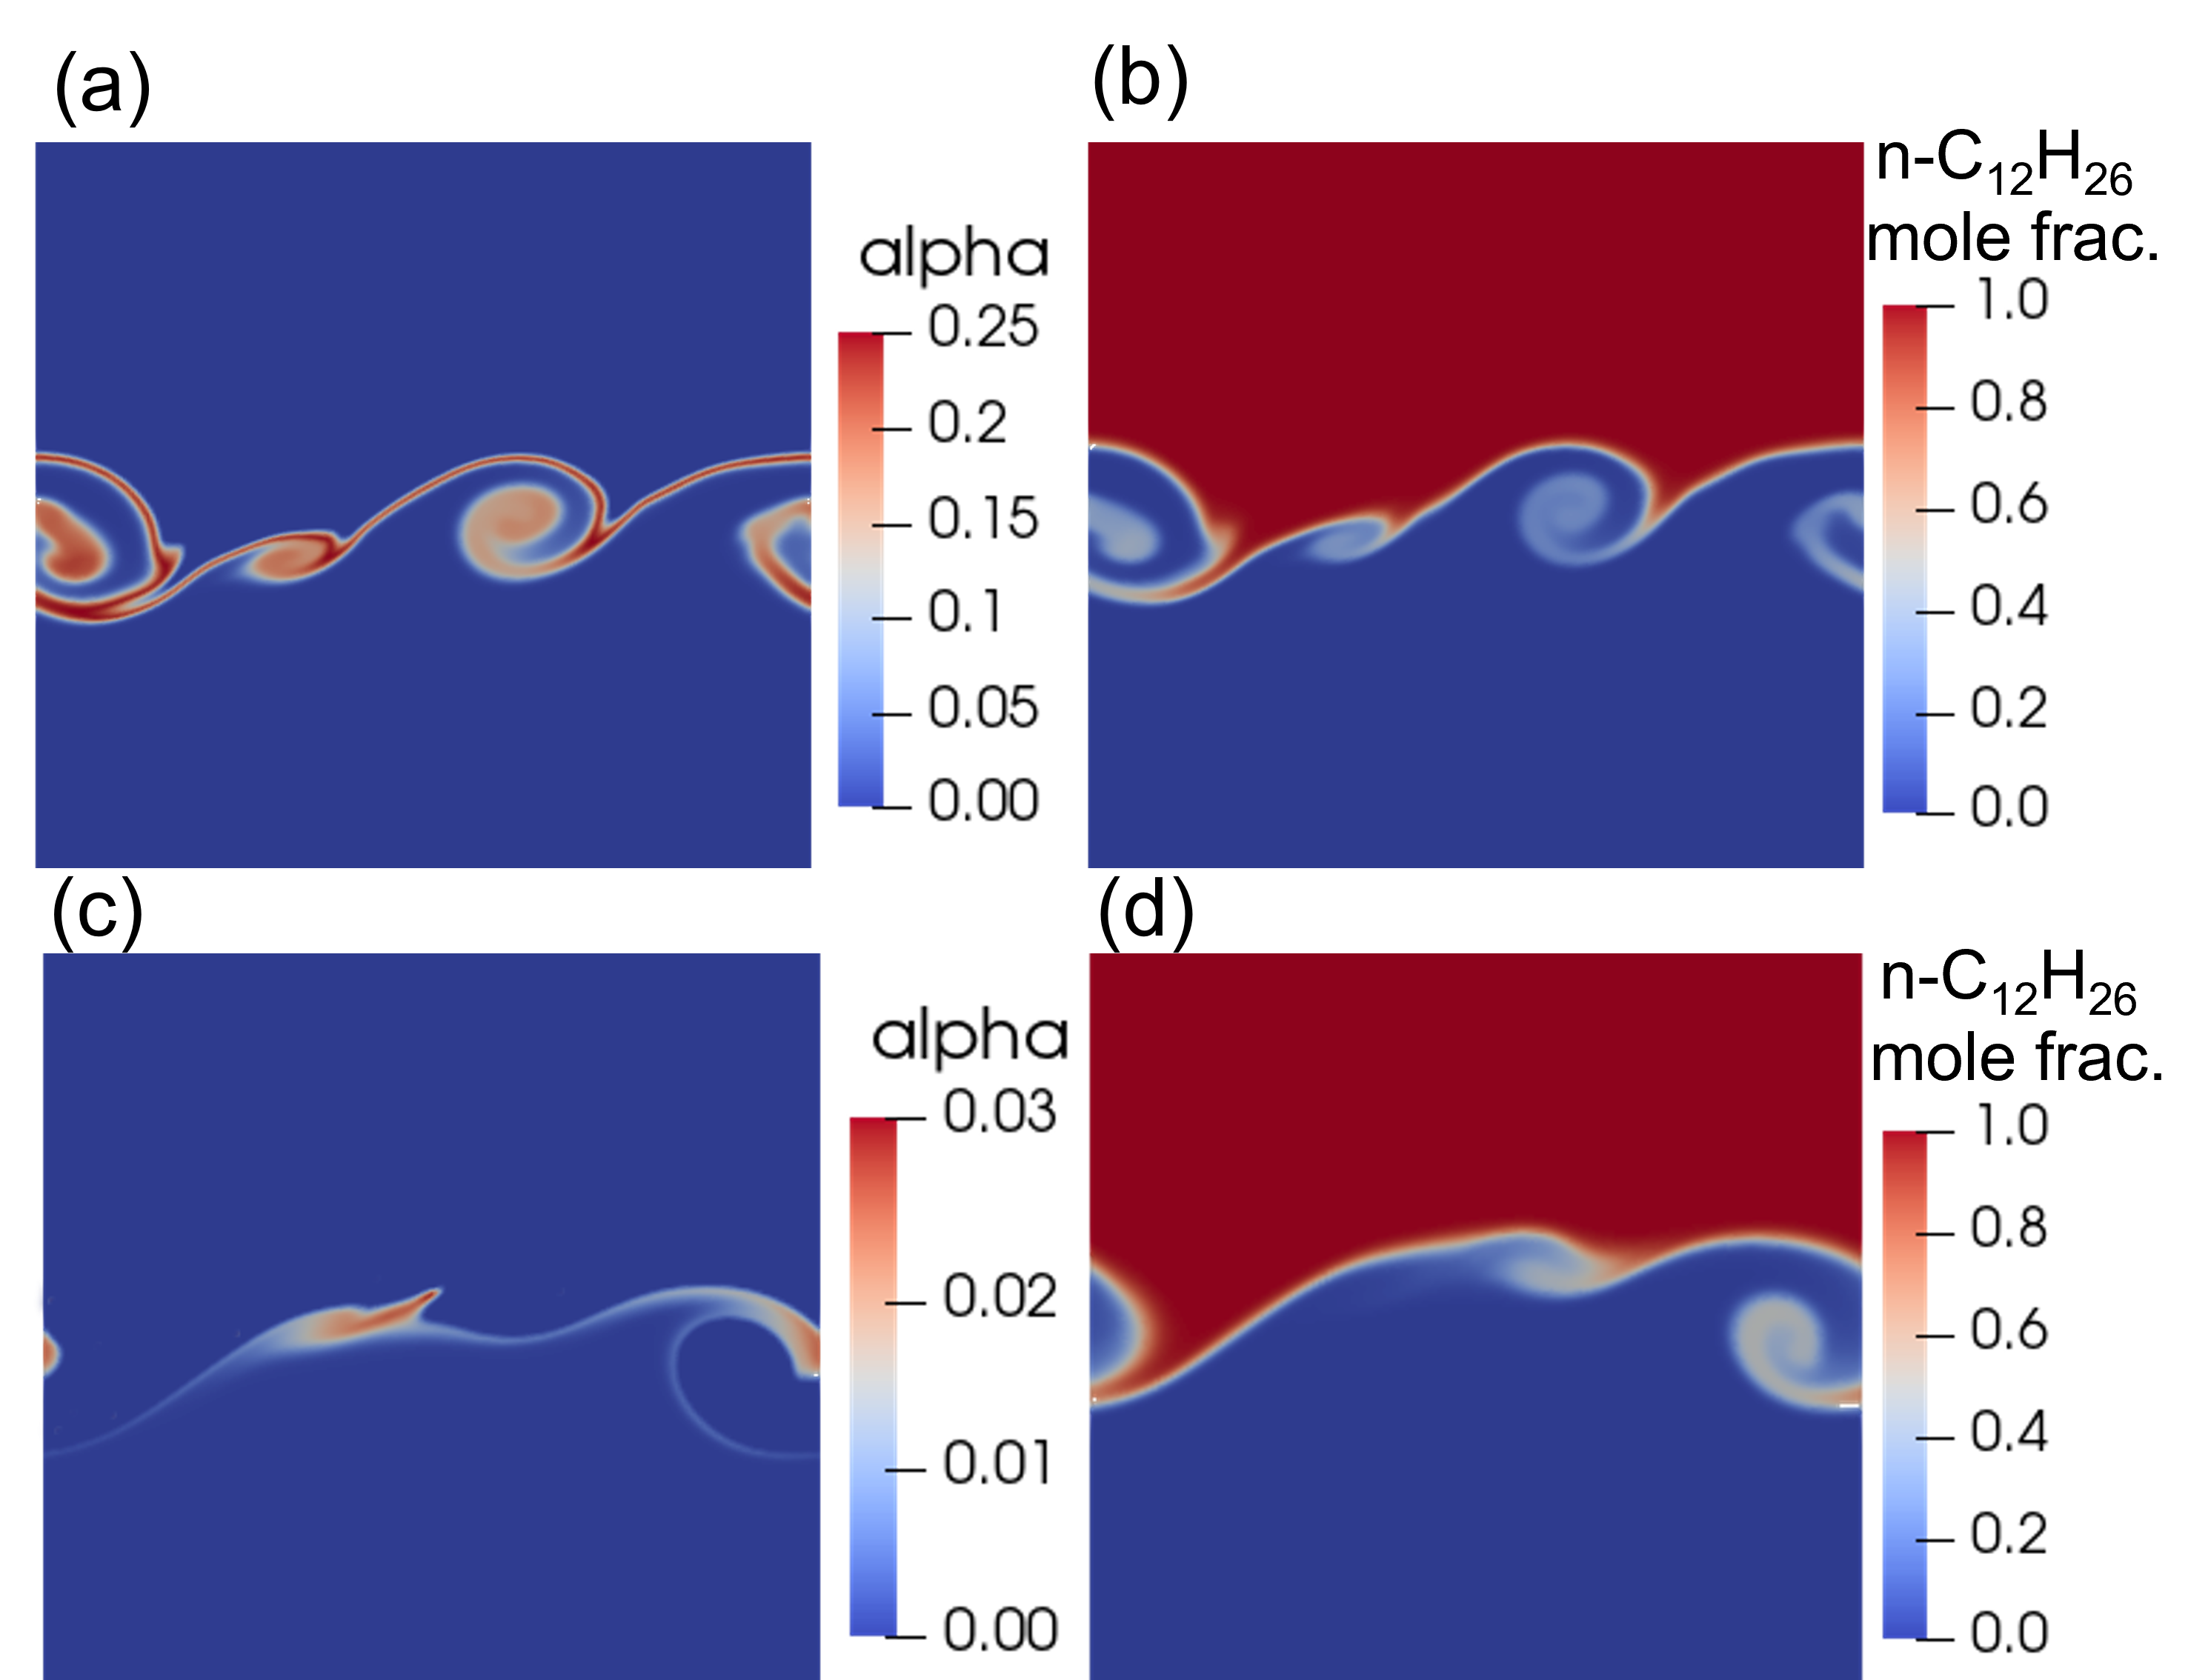
\includegraphics[width=0.60\linewidth]{TML_2_cases2.png}
%\includegraphics[width=0.35\linewidth]{C12_39_2e_7.png}
%\includegraphics[width=0.35\linewidth]{C12_71_3.6e_7.png}

%\includegraphics[width=0.35\linewidth]{alpha_39_2e_7.png}
%\includegraphics[width=0.35\linewidth]{alpha_71_3.6e_7.png}
\caption{3D temporal mixing layer (TML) contours at $\tau = 45$ (in which $\tau = t \Delta U/ \delta_{\omega,0}$). Top (a,b): Case 1; Bottom (c,d): Case 2. Left (a,c): $\alpha$ (which is the indicator of the two-phase interface: $\alpha = \beta(1-\beta)$, where $\beta$ is vapor mole fraction); Right (b,d): mole fraction of \ce{n-C12H26}.}
\label{TML_3D_result} 
\end{figure}
The distinction between Case 1 and Case 2 can be better understood by analyzing through a phase diagram. Since the pressure variation in the TML simulation is relatively small, a temperature-mole fraction (T-X) diagram is employed to compare the two cases. In Fig.~\ref{TML_TX}, the phase boundaries at 50 bar and 40 bar serve as reference lines for the two-phase region. In Case 1, the lower initial temperature of \ce{n-C12H26} (600 K) causes the thermodynamic states of the mixing layer fluid ($X_{C_{12}H_{26}}$ within the range of 0.2-0.6) to overlap with the two-phase region, resulting in significant phase separation. However, in Case 2, the higher temperature of \ce{n-C12H26} (800 K) leads to points with $X_{C_{12}H_{26}}>0.3$ having temperatures above the two-phase boundary, thereby preventing phase separation in this region. Fig.~\ref{TML_TX} illustrates that the temperature of the phase boundary increases rapidly within the range of $X_{C_{12}H_{26}}<0.2$, making it difficult for the fluid in this region to remain outside the two-phase region in terms of thermodynamic properties. Consequently, Case 2 still exhibits weak phase separation. We further conducted tests with even higher initial \ce{n-C12H26} temperatures (up to 1200 K), resulting in further weakening of the phase separation, although it still persists.

\begin{figure}[htbp]
\centering
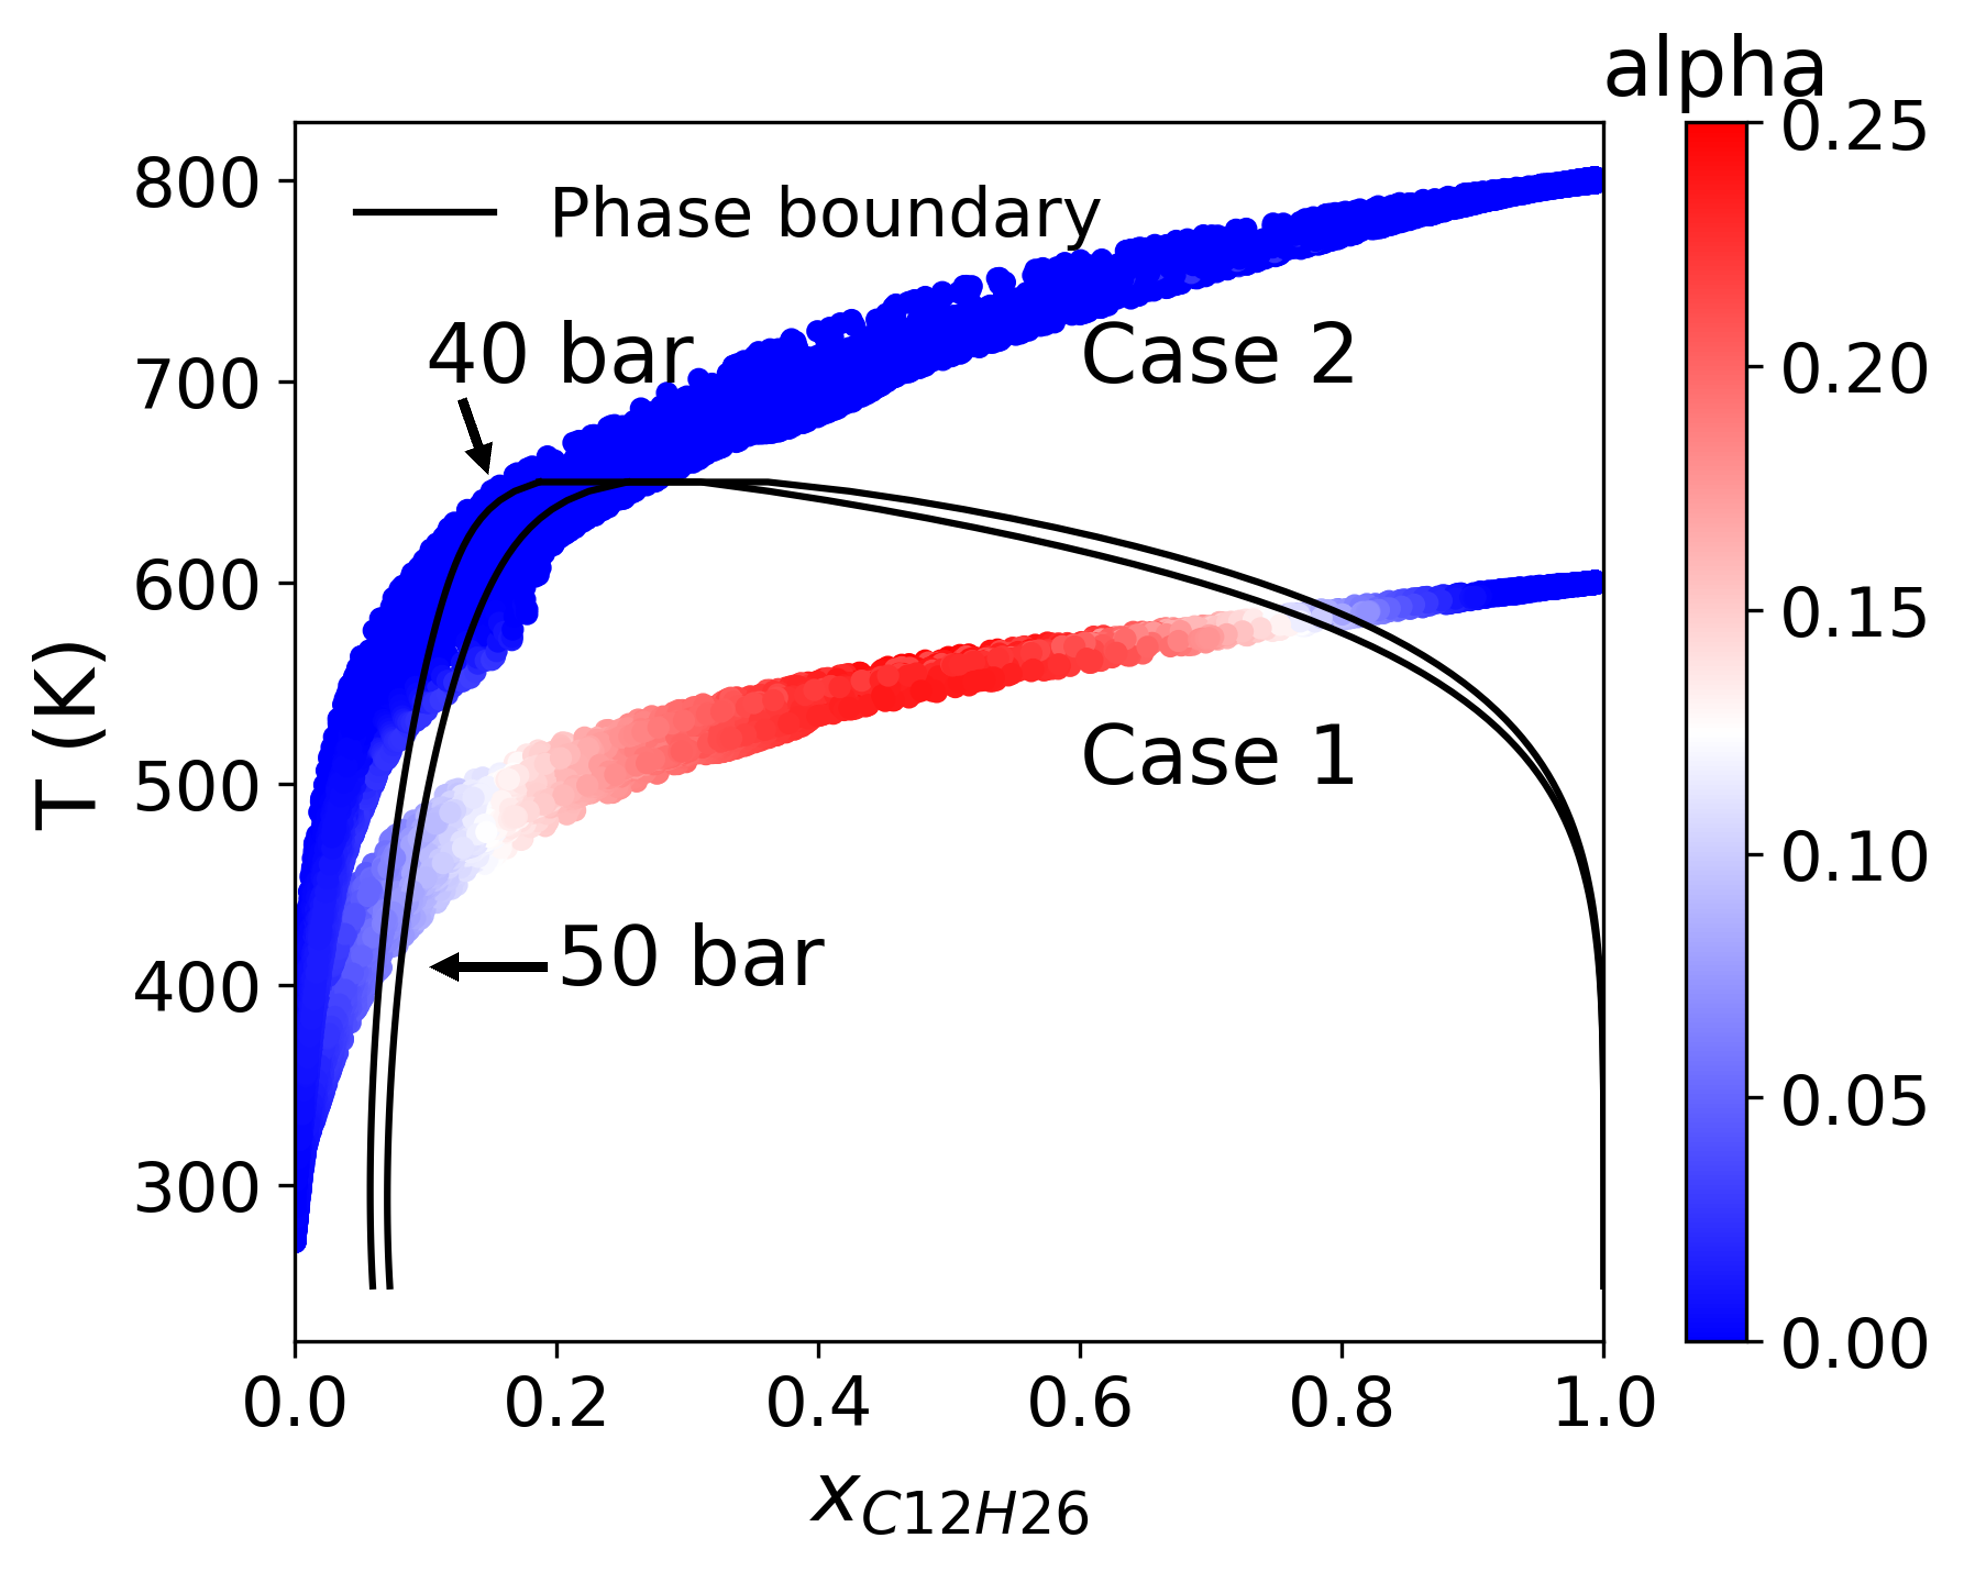
\includegraphics[width=0.45\linewidth]{TML_TX2.png}
\caption{The temperature-mole fraction (T-X) phase diagram of temporal mixing layer (TML) simulation: the phase boundary of \ce{N2}/\ce{C12H26} at 50 bar is shown in the plot as a solid black curve, and the region it encloses is the two-phase region at 50 bar.}
\label{TML_TX} 
\end{figure}

Fig.~\ref{TML_3D_performace} shows the performance of the ISAT-VLE method in the 3D simulation of Case 1. The simulation utilizes 128 CPU cores, and the CPU times presented in the figure represent the maximum time cost among all MPI processes at each time step. Initially, the ISAT-VLE method provides a speed-up of approximately 28 times. However, as the simulation progresses and more vortices form, the computational cost of ISAT-VLE increases. At the final time step, ISAT-VLE only achieves a speed-up of 1.5 times. This performance is very different from the one shown in Fig.~\ref{TML_PE}(a). The discrepancy arises because the ISAT-VLE method is more expensive in the interface region than the pure component region. This difference is attributable to the increased dispersion of thermodynamic states in the thermodynamic property space, necessitating more direct calculations of the VLE model. The distinct characteristics of different regions in the computational domain prevent the computing cores from synchronizing effectively. Consequently, the impact of data synchronization and communication between the computing cores becomes more pronounced, leading to longer waiting times. These challenges make it hard to accurately evaluate the performance of ISAT. Moreover, these issues are not solely related to the ISAT-VLE model but are also influenced by the overall CFD solver and hardware. Therefore, the 2D results provide a better reflection of the performance of ISAT-VLE.


%This difference between the different regions in the computational domain leads to calculations that the computing cores cannot synchronize, which makes the impact of data synchronization and communication between the different computing cores greater, resulting in more waiting times, and these factors make it difficult to test the performance of ISAT. These problems are not only related to the ISAT-VLE model, but also affected by the entire CFD solver and hardware design, so the results here are only a demonstration, and the 2D results can better reflect the performance of ISAT-VLE, %Since computational time depends on the slowest core, compared to serial simulation (Fig.~\ref{TML_PE}(a)), ISAT-VLE performance in parallel simulation is more sensitive to the local cost. In total, we still obtain a speed-up factor of about 3 using the ISAT-VLE method. 

\begin{figure}[htbp]
\centering
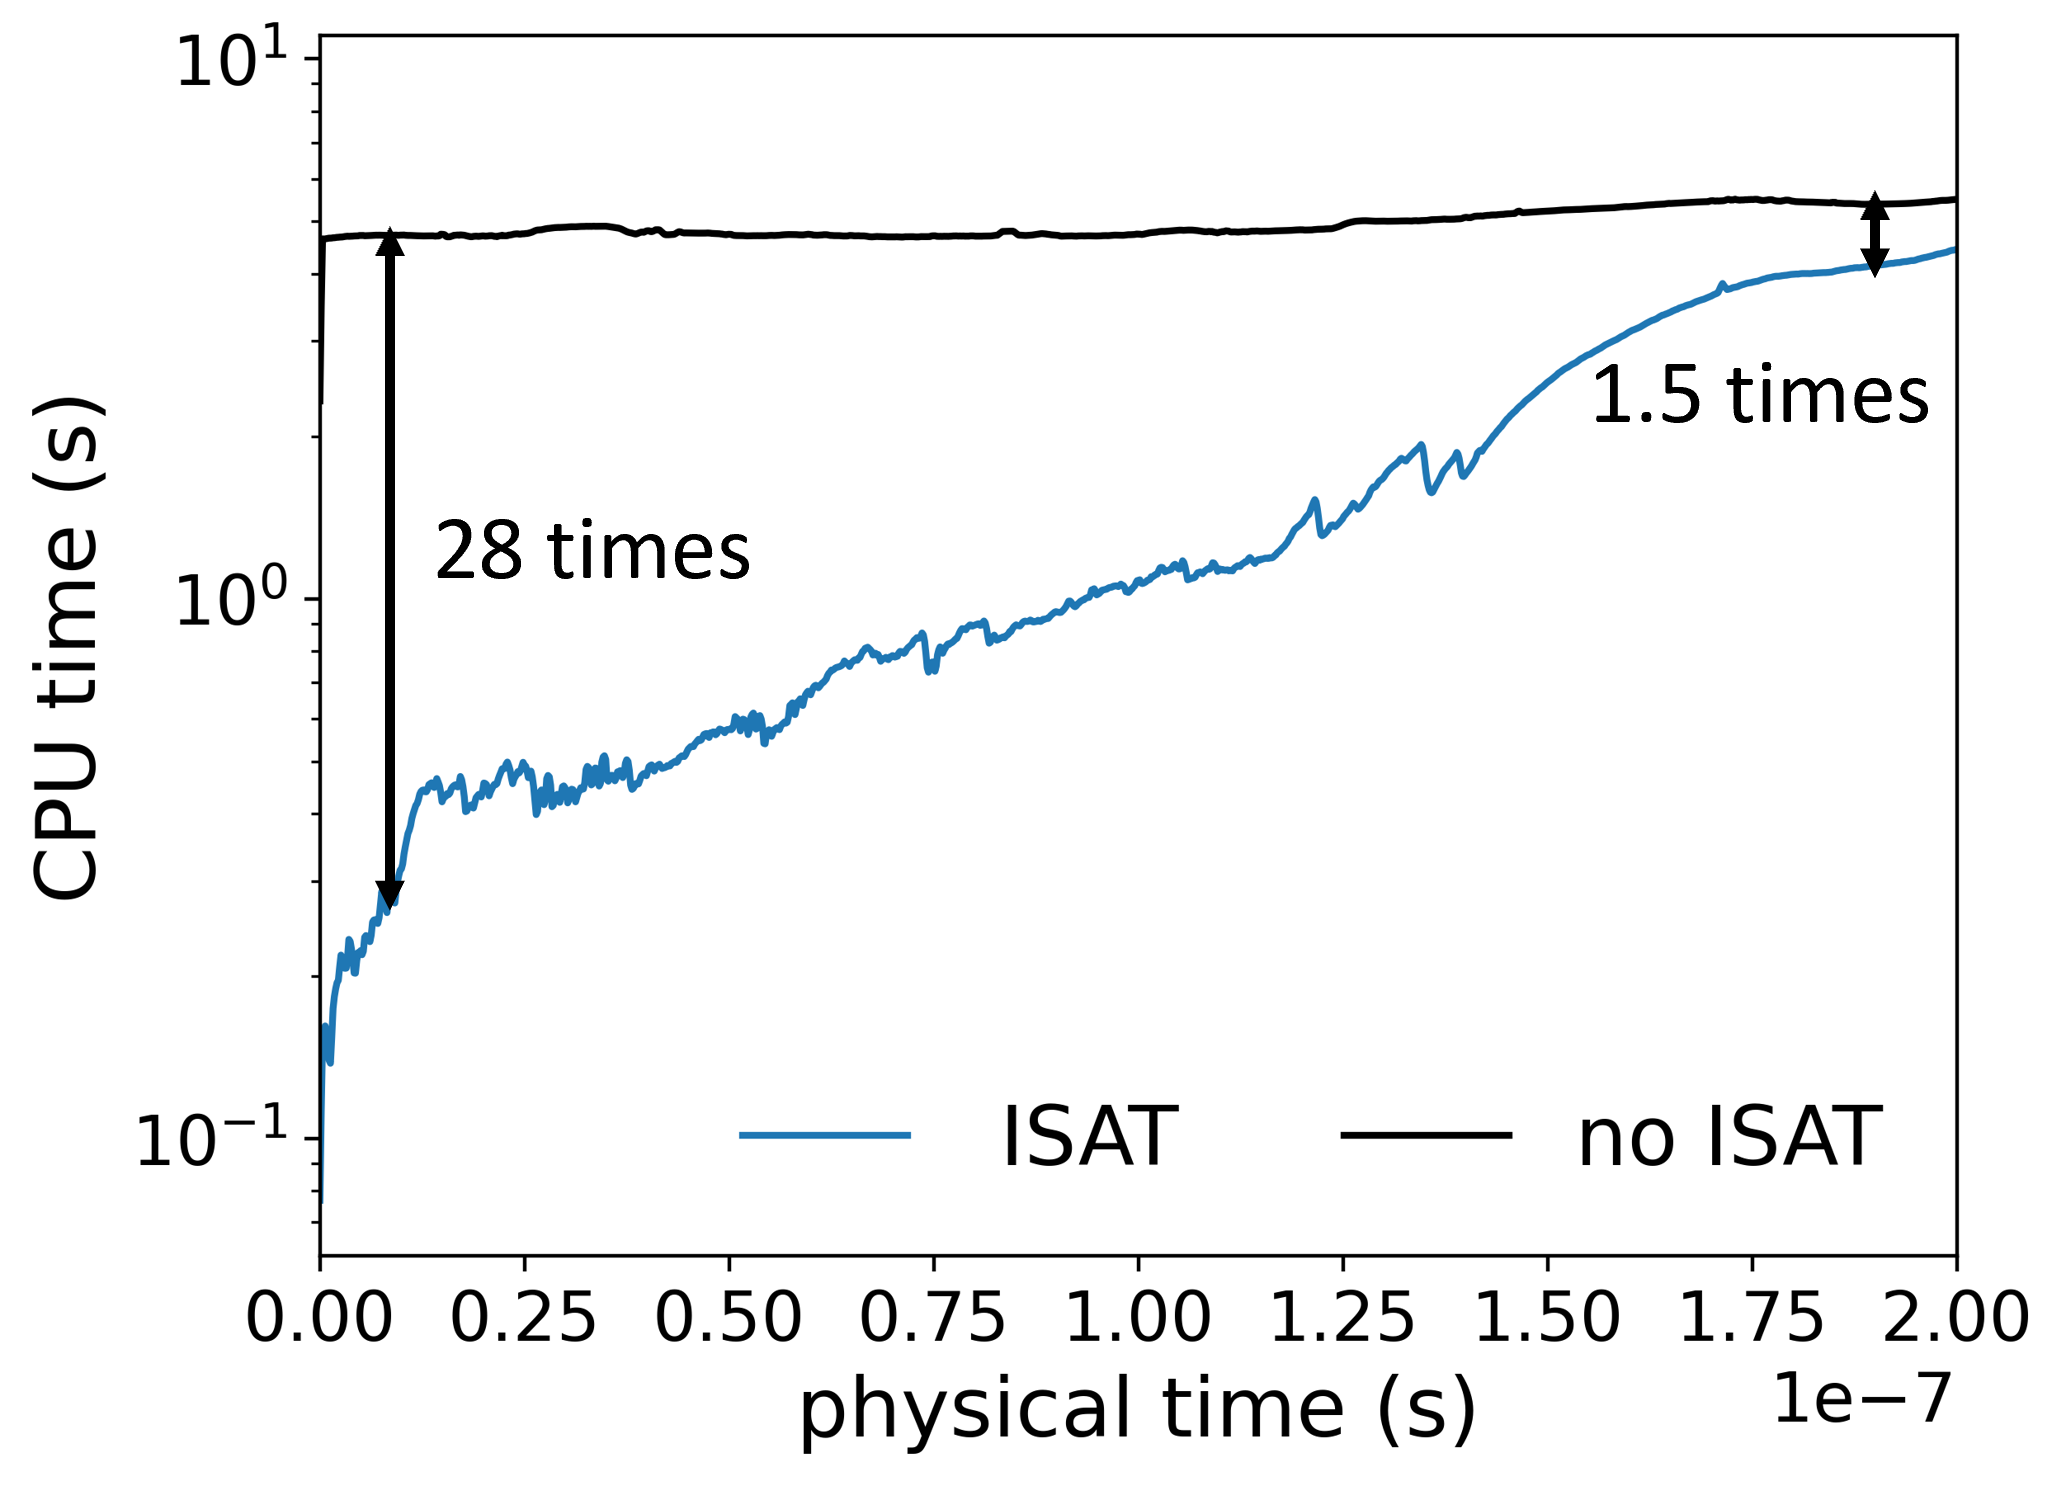
\includegraphics[width=0.45\linewidth]{time_p_TML_m.png}
\caption{Performance of the ISAT-VLE method in the 3D simulation of the temporal mixing layer (TML).}
\label{TML_3D_performace} 
\end{figure}




\subsection{Transcritical shock-droplet interaction}
\label{sec:SD}

In this section, transcritical shock-droplet interaction simulations are conducted to investigate the performance and error control of the ISAT-VLE method. The geometry of the initial setting is shown in Fig.~\ref{SD_GEO}, where $L=2$ mm and $l=0.5$ mm. A droplet of \ce{n-C12H26} with a diameter $d=0.25$ is positioned at the center of the domain, and the domain is filled with \ce{N2}. The initial pressure is set to 200 bar, and a high-pressure region of 800 bar is positioned on the left to generate a shock wave. The interfacial mass fraction of \ce{N2} is initialized using $\tanh(x/\omega)$, where $\omega=2 \times 10^{-6}$. The performance of ISAT-VLE is tested through both 2D and 3D simulations. In both cases, a uniform mesh size of $256\times256$ is utilized in the x-y plane. For the 3D simulations, the z direction consists of 256 uniformly spaced grid intervals. 


\begin{figure}[htbp]
\centering
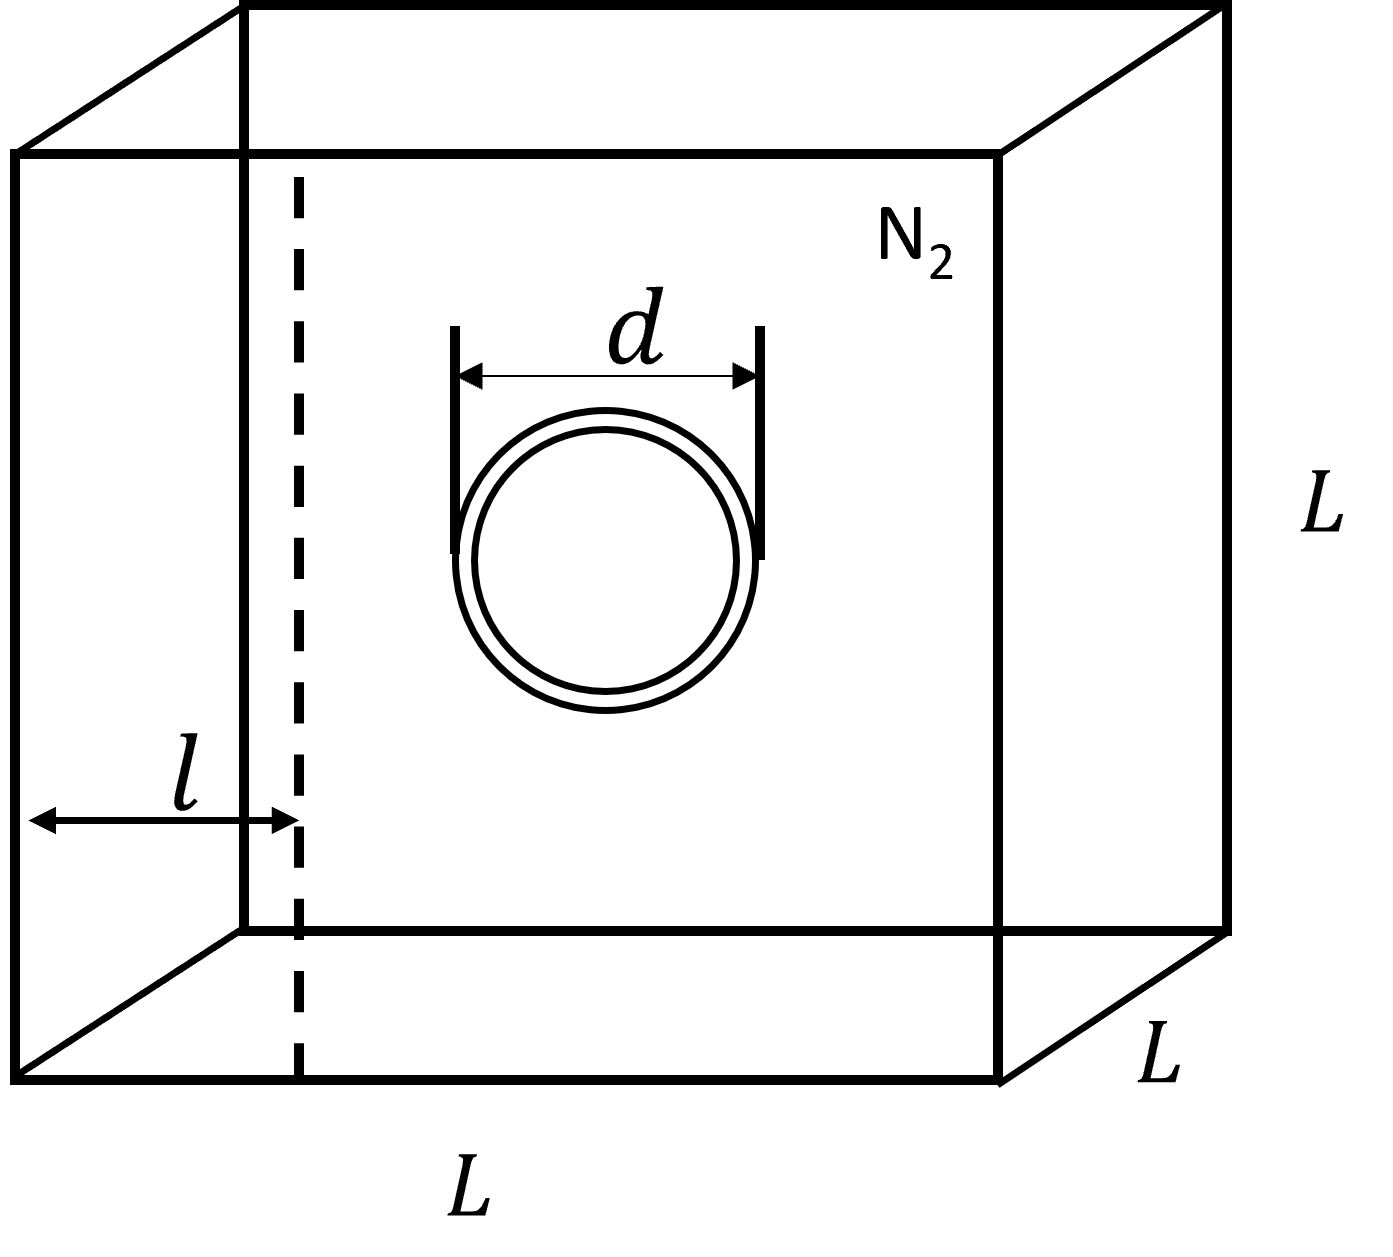
\includegraphics[width=0.35\linewidth]{ShockDrop_sc.png}
\hspace{.7in}
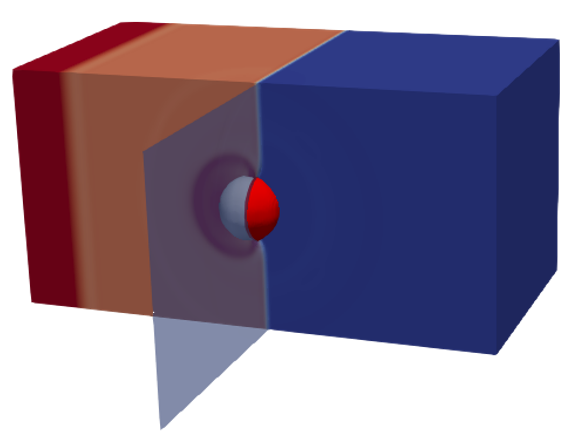
\includegraphics[width=0.30\linewidth]{2C_3d2.0080_s.png}
\caption{Left: geometry of the shock-droplet interaction simulations. The computational domain is of squared shape with side $L=2$mm. A high-pressure region with thickness $l=0.5$ mm is used to generate a shock wave. Droplet diameter: $d=0.25$ Right: pressure contours of the 3D shock-droplet interaction. Shock front: iso-surface of $P=30$ MPa; White color on the droplet surface: iso-surface of $Y_{C_{12}H_{26}}=0.7$; Red color on the droplet surface: iso-surface of $\beta =0.9$ to visualize the subcritical interface.}
\label{SD_GEO} 
\end{figure}

\subsubsection{ISAT-VLE's error control and tolerance in 2D simulations}
2D simulations are utilized to evaluate the error control of ISAT-VLE and select an appropriate error tolerance for later simulations. Throughout the entire computational domain, the initial temperature is set to 565 K, which is chosen specifically to examine the phase change effect in a multi-component droplet (refer to Sec.\ref{sec:SD_3D}). Initially, the fully conservative (FC) method results are presented. A range of error tolerance values are employed to assess performance, where the error tolerance $(T_{tol},p_{tol},\beta_{tol},c_{tol})$ is scaled by a factor $k$: specifically, the error tolerance values are set as $k (10^2, 10^7, 1, 10^2)$. The magnitude of these tolerances is based on the properties observed in these simulations. The error tolerance cases run until a physical time of $1\times 10^{-6}$s, at which point the shock wave has completely passed through the droplet. Fig.~\ref{droplet_PE}(a) illustrates the performance of ISAT-VLE. The top red line represents the CPU time cost of the VLE model without ISAT at each time step, while the blue dotted line corresponds to the CPU time cost of the remaining parts of the CFD solver. Both lines are insensitive to time. Compared with the rest part of the CFD solver, the VLE model without ISAT is computationally expensive, consistently utilizing around 90\% of the computational resources throughout this simulation. Prior to the interaction between the shock wave and the droplet, the computational costs of all ISAT-VLE cases with varying tolerances are similar. This is attributed to the simple thermodynamic states involved, where a limited data set in the ISAT-VLE table is sufficient to provide accurate approximations. Therefore, in this stage, the ISAT-VLE method exhibits excellent performance, with a speed-up factor of approximately 50, and the error tolerance has minimal impact on performance. As the shock-droplet interaction commences, the computational cost begins to increase, and the influence of the error tolerance becomes evident. Cases with larger tolerances demonstrate faster computation, and by a physical time of $1.5\times 10^{-6}$s, when the droplet has passed through the shock wave, the CPU times stabilize. At this stage, the case with the largest tolerance is approximately 22 times faster than the VLE model without ISAT, while even the slowest case is still around 11 times faster. 

The normalized ISAT error for the case with $k=3\times10^{-2}$ is depicted in Fig.~\ref{droplet_PE}(b). The error is normalized by its tolerance, and the dashed line represents an error equal to the normalized tolerance (error = 1), below which the error is controlled within the specified tolerance. The average error is three orders of magnitude smaller than the tolerance, and the maximum error is also within the tolerance. Table~\ref{droplet_FC_table} presents the errors and speed-up factors for all cases. Considering the initial pressure range (200 - 800 bar) and temperature (565 K) settings, the errors are acceptable, staying within 2\% for all different tolerances. For subsequent shock-droplet simulations, we choose $k=2 \times 10^{-3}$, which maintains the error within 1\% and provides sufficient accuracy.



\begin{figure}[htbp]
\centering
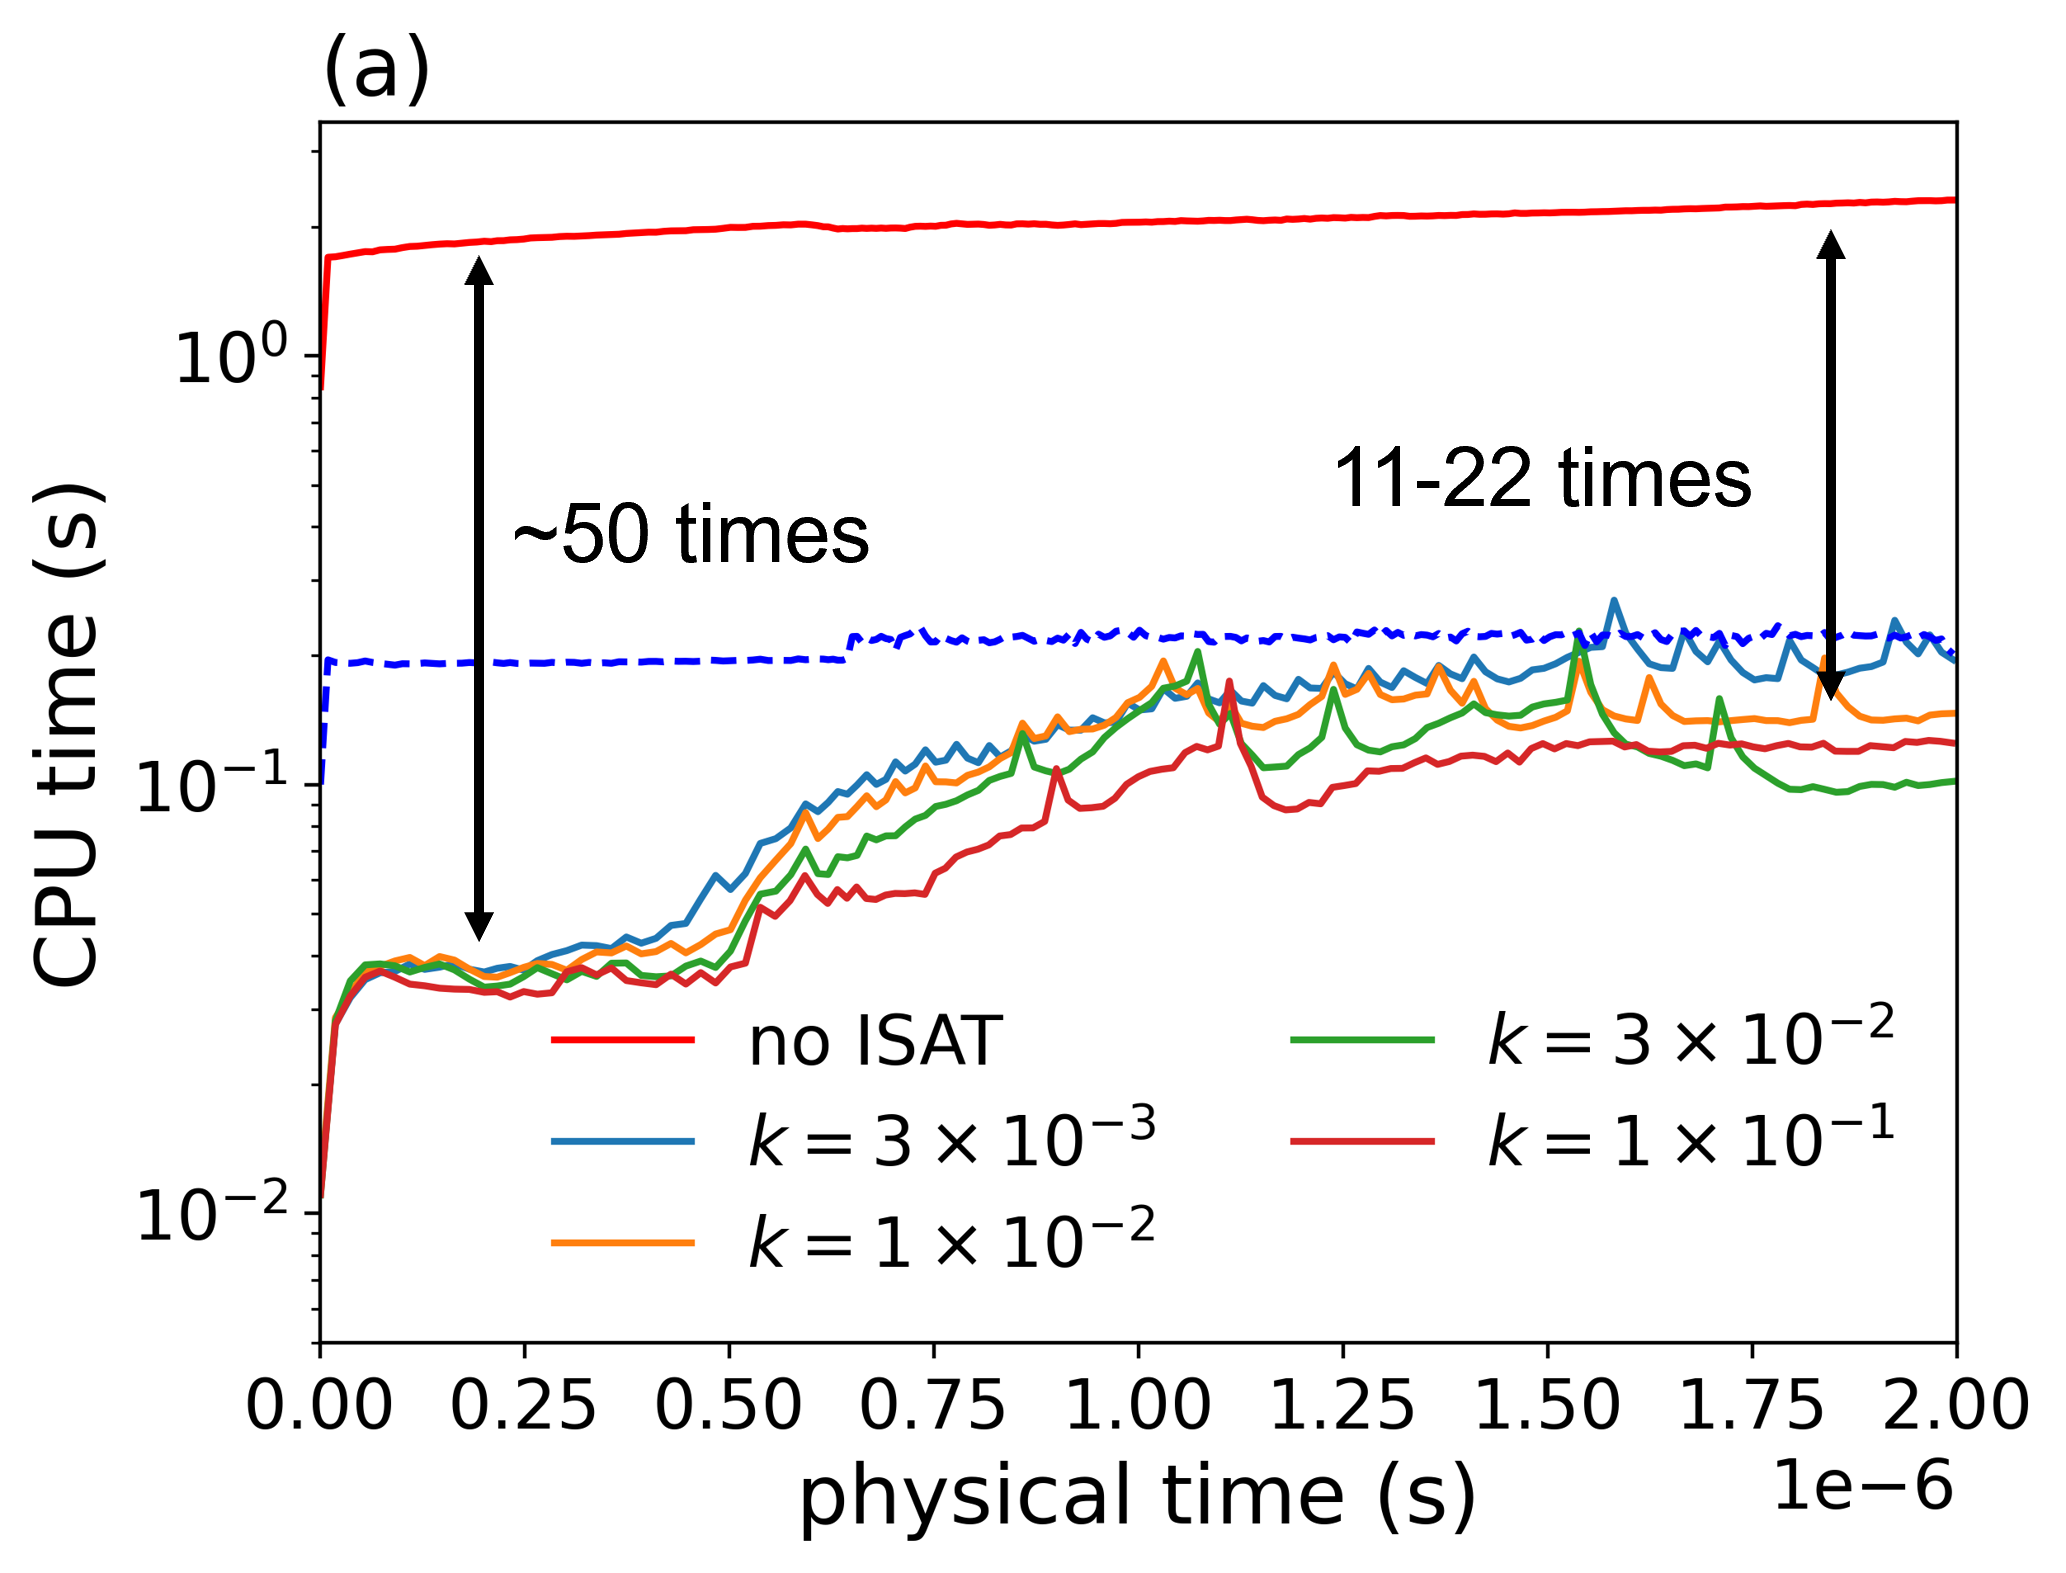
\includegraphics[width=0.45\linewidth]{time_droplet_C_2d_2_p.png}
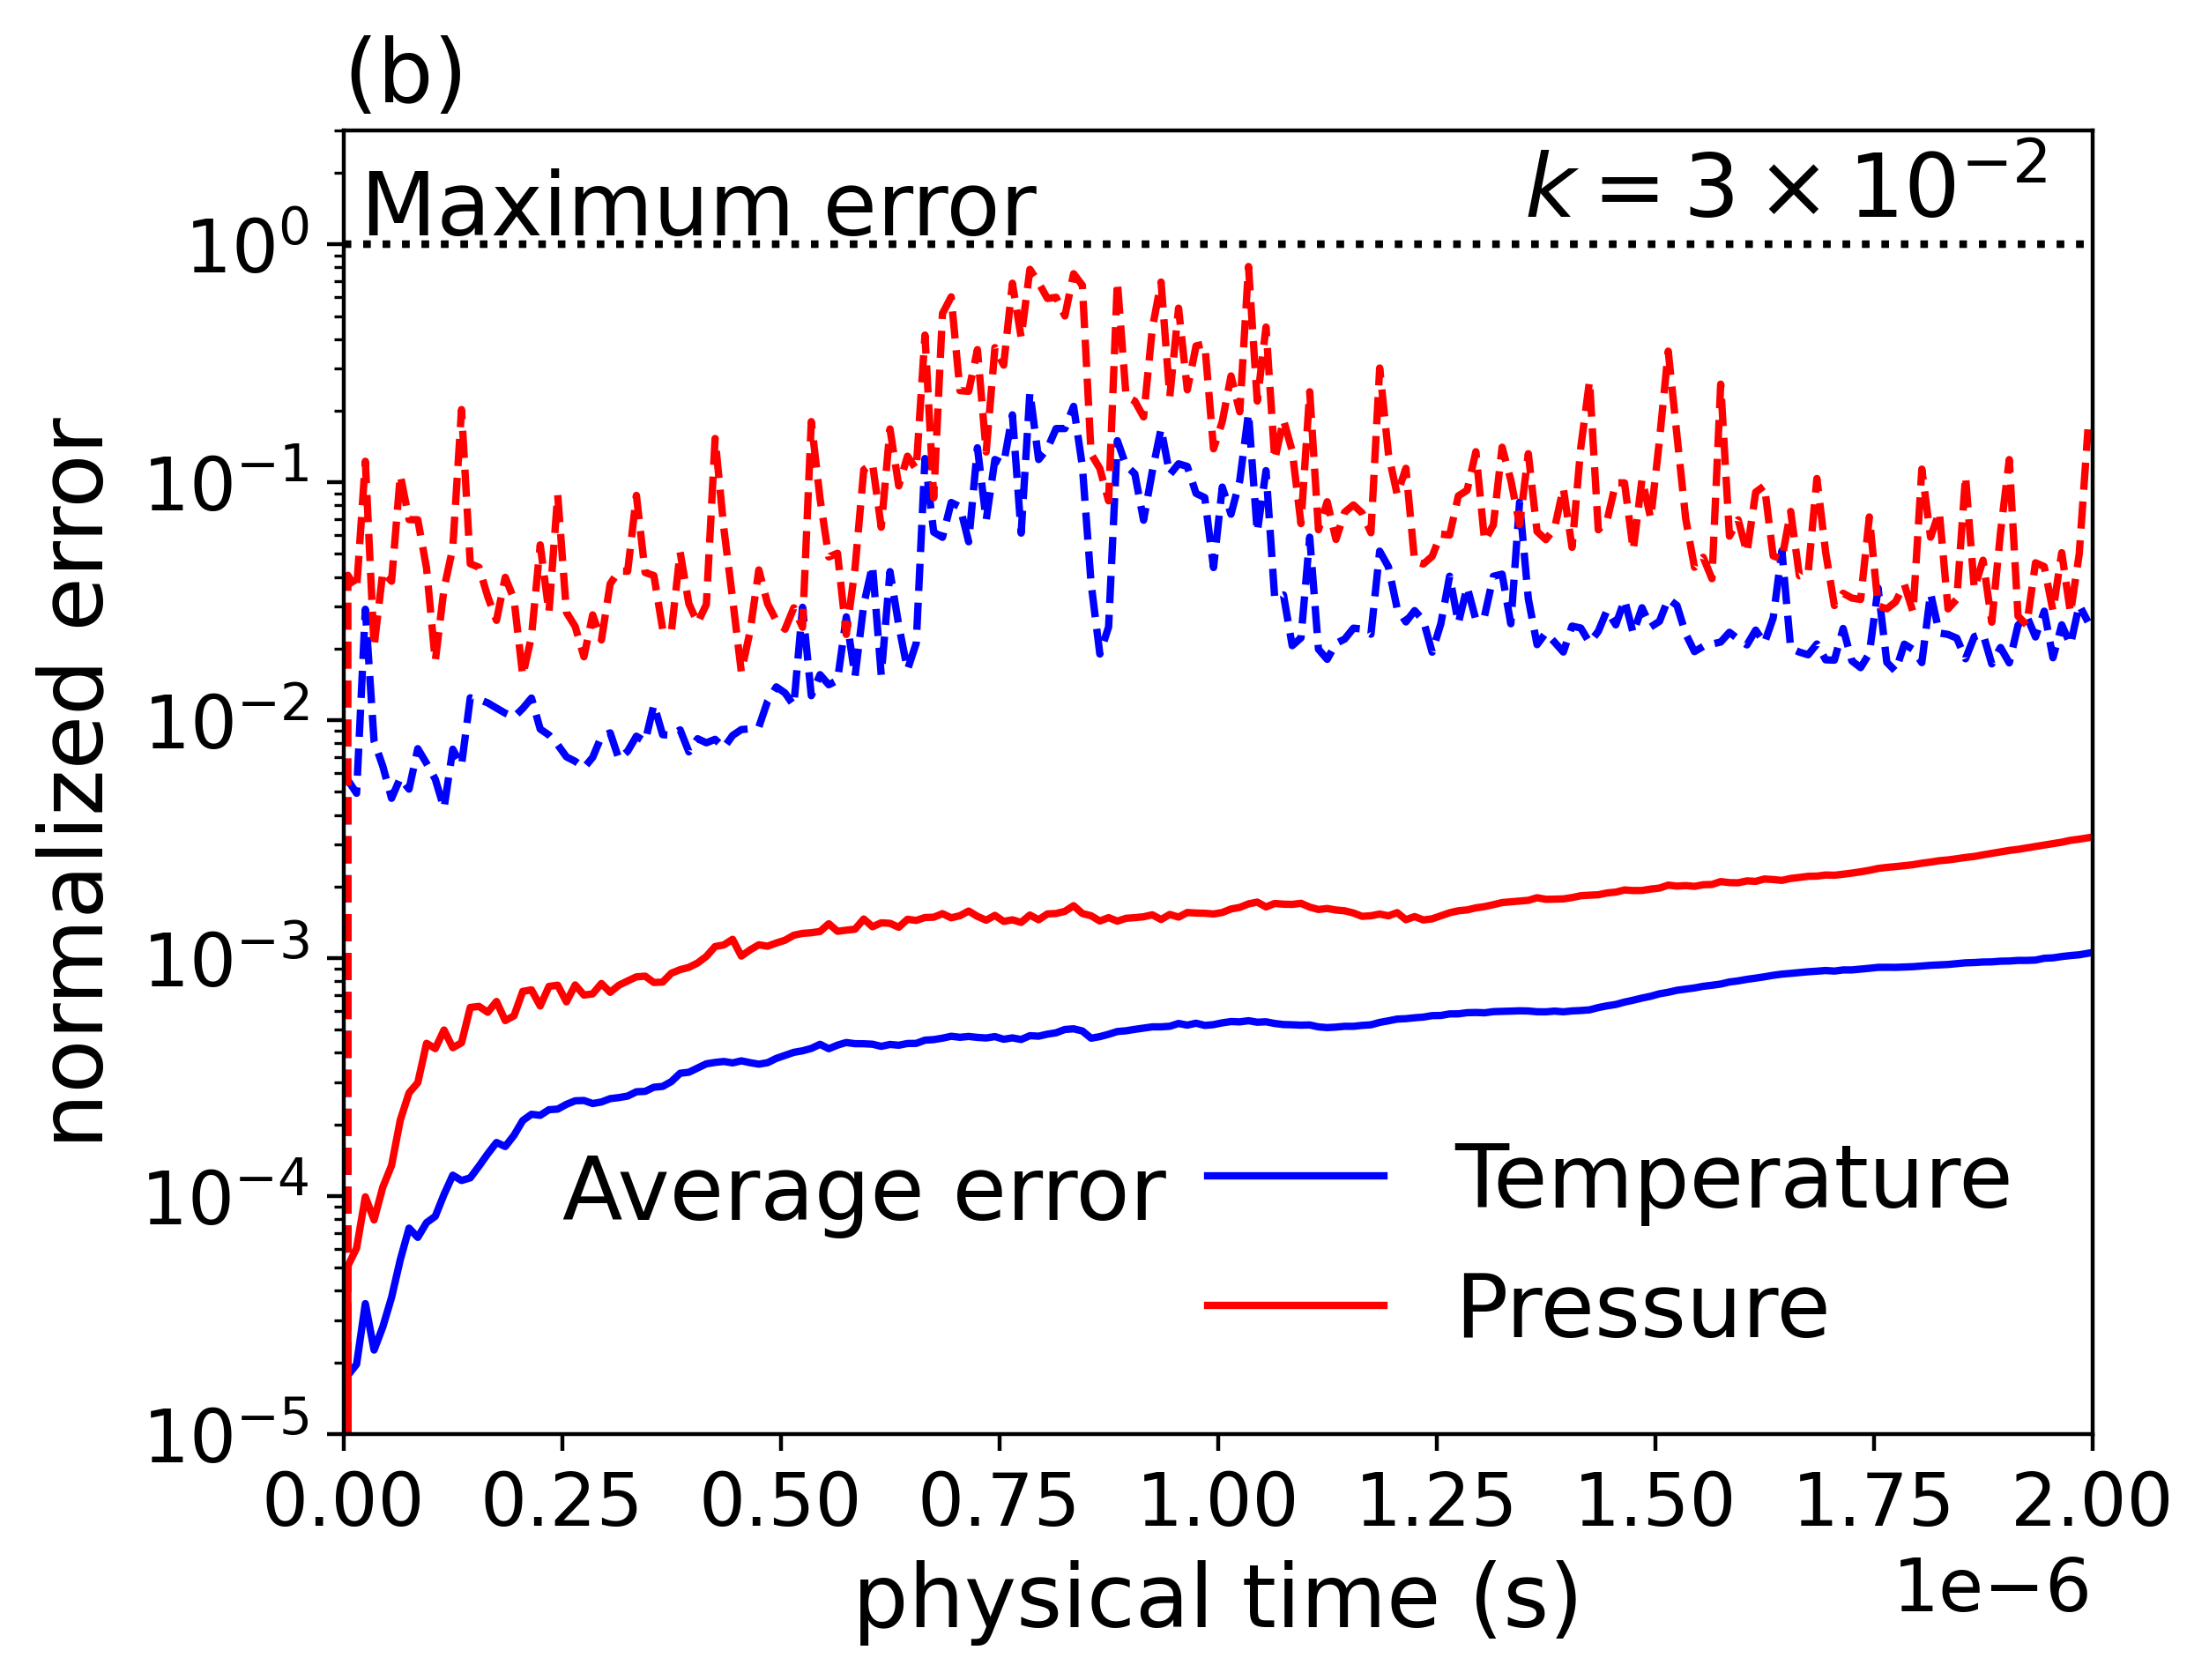
\includegraphics[width=0.45\linewidth]{error_droplet_C_2d.png}
\caption{(a) Performance of the ISAT-VLE method in the transcritical shock-droplet interaction simulation using the fully compressible (FC) scheme: the blue dotted line is the CPU time of all other parts of CFD solver, except the VLE model; the red line is the CPU time of VLE model without ISAT, and 4 lines of ISAT-VLE model with different tolerances ($k$) are provided. (b) The normalized error of the ISAT-VLE method with an error control of $k = 3 \times 10^{-2}$.}
\label{droplet_PE} 
\end{figure}


%\begin{table}[width=.9\linewidth,cols=4,pos=h]
%\caption{The performance and error of the ISAT-VLE method in the transcritical shock-droplet interaction cases with different error tolerance.}\label{droplet_FC_table}
%\begin{tabular*}{\tblwidth}{@{} L|LLLLL@{} }
%\toprule
%$k$                         & $3\times 10^{-3}$    & $1\times 10^{-2}$    &$3\times 10^{-2}$    & $1\times 10^{-1}$\\
%\midrule
%Speed-up                    & 15.3                 & 17.9                 & 20.9                &  23.8\\
%$P$ mean error (bar)        & $2.4\times 10^{-4}$  & $1.8\times 10^{-3}$  & $9.6\times 10^{-3}$ & $8.8\times 10^{-2}$\\
%$P$ max error (bar)         & 0.26                 & 0.86                 & 2.4                 & 7.7 \\
%$P$ max relative error (\%) & 0.07                 & 0.2                  & 0.57                & 1.9 \\
%$T$ mean error (K)          & $1.0\times 10^{-4}$  & $6.4\times 10^{-4}$  & $3.1\times 10^{-3}$ & $3.5\times 10^{-2}$\\
%$T$ max error (K)           & 0.074                & 0.17                 & 0.71                & 2.2\\
%$T$ max relative error (\%) & 0.012                & 0.029                & 0.12                & 0.36 \\
%\bottomrule
%\end{tabular*}
%\end{table}

\begin{table}%[width=.9\linewidth,cols=4,pos=h]
\caption{The performance and error of the ISAT-VLE method in the transcritical shock-droplet interaction cases with different error tolerance.}\label{droplet_FC_table}
\begin{tabular*}{0.8\textwidth}{@{} l|lllll@{} }
\toprule
$k$                         & $3\times 10^{-3}$    & $1\times 10^{-2}$    &$3\times 10^{-2}$    & $1\times 10^{-1}$\\
\midrule
Speed-up                    & 15.3                 & 17.9                 & 20.9                &  23.8\\
$P$ mean error (bar)        & $2.4\times 10^{-4}$  & $1.8\times 10^{-3}$  & $9.6\times 10^{-3}$ & $8.8\times 10^{-2}$\\
$P$ max error (bar)         & 0.26                 & 0.86                 & 2.4                 & 7.7 \\
$P$ max relative error (\%) & 0.07                 & 0.2                  & 0.57                & 1.9 \\
$T$ mean error (K)          & $1.0\times 10^{-4}$  & $6.4\times 10^{-4}$  & $3.1\times 10^{-3}$ & $3.5\times 10^{-2}$\\
$T$ max error (K)           & 0.074                & 0.17                 & 0.71                & 2.2\\
$T$ max relative error (\%) & 0.012                & 0.029                & 0.12                & 0.36 \\
\bottomrule
\end{tabular*}
\end{table}

\subsubsection{Double flux scheme's behavior in 2D simulations}
\label{sec:DF}
We proceeded to perform a simulation using the double flux (DF) scheme to compare its behavior with the FC scheme. The ISAT-VLE error tolerance is set as $(T_{tol},e_{tol},\beta_{tol},c_{tol})= k (10^2, 10^4, 1, 10^2)$. Similar to the FC method,  performance improves when a larger tolerance is employed (Fig.~\ref{droplet_PE_D}(a)), but in comparison, the DF scheme runs even faster. Fig.~\ref{droplet_PE_D}(b) displays the normalized error (at $k=3 \times 10^{-2}$) It can be observed that the average error is controlled three orders of magnitude below the error tolerance. Although the maximum error cannot be entirely controlled within the tolerance due to the high non-linearity of the VLE system, the overall error remains within an acceptable range. The error and performance are listed in Tab.~\ref{droplet_DF_table}. When compared to the FC solver, the ISAT implementation in the DF solver achieves larger speedup factors ranging from 40 to 60, and exhibits significantly smaller pressure errors but slightly larger temperature errors. This discrepancy arises because, in the DF method, the pressure is directly obtained from the CFD solver, and its error is only influenced by the tabulation error of other properties, resulting in minimal pressure error. However, the DF scheme introduces stronger temperature oscillations (as depicted in Fig.~\ref{droplet_DC_compare} and discussed below), which contribute to an increased temperature error. Additionally, the double flux technique suppresses pressure oscillations, simplifying the thermal state and consequently leading to a larger speedup factor.


%\begin{table}[width=.9\linewidth,cols=4,pos=h]
%\caption{The performance and error of the ISAT-VLE method using DF in the transcritical shock-droplet interaction cases with different error tolerance.}\label{droplet_DF_table}
%\begin{tabular*}{\tblwidth}{@{} L|LLLLL@{} }
%\toprule
%$k$                        & $3\times 10^{-3}$   & $1\times 10^{-2}$    &$3\times 10^{-2}$    & $1\times 10^{-1}$\\
%\midrule
%Speed-up                   & 41.1                & 50.0                 & 60.9                & 63.9\\
%$P$ mean error (bar)       & $6.7\times 10^{-5}$ & $2.2\times 10^{-4}$  & $2.4\times 10^{-4}$ & $1.2\times 10^{-3}$\\
%$P$ max error (bar)        & $3.7\times 10^{-3}$ & $7.4\times 10^{-3}$  & $8.4\times 10^{-3}$ & $5.2\times 10^{-2}$ \\
%$P$ max relative error (\%)& 0.001               & 0.002                & 0.003               & 0.016 \\
%$T$ mean error (K)         & $3.9\times 10^{-3}$ & $1.1\times 10^{-3}$  & $2.8\times 10^{-3}$ & $7.5\times 10^{-3}$\\
%$T$ max error (K)          & 0.14                & 4.43                 & 4.52                & 9.39\\
%$T$ max relative error (\%)& 0.02                & 0.76                 & 0.78                & 1.5 \\
%\bottomrule 
%\end{tabular*}
%\end{table}

\begin{table}%[width=.9\linewidth,cols=4,pos=h]
\caption{The performance and error of the ISAT-VLE method using DF in the transcritical shock-droplet interaction cases with different error tolerance.}\label{droplet_DF_table}
\begin{tabular*}{0.8\textwidth}{@{} l|lllll@{} }
\toprule
$k$                        & $3\times 10^{-3}$   & $1\times 10^{-2}$    &$3\times 10^{-2}$    & $1\times 10^{-1}$\\
\midrule
Speed-up                   & 41.1                & 50.0                 & 60.9                & 63.9\\
$P$ mean error (bar)       & $6.7\times 10^{-5}$ & $2.2\times 10^{-4}$  & $2.4\times 10^{-4}$ & $1.2\times 10^{-3}$\\
$P$ max error (bar)        & $3.7\times 10^{-3}$ & $7.4\times 10^{-3}$  & $8.4\times 10^{-3}$ & $5.2\times 10^{-2}$ \\
$P$ max relative error (\%)& 0.001               & 0.002                & 0.003               & 0.016 \\
$T$ mean error (K)         & $3.9\times 10^{-3}$ & $1.1\times 10^{-3}$  & $2.8\times 10^{-3}$ & $7.5\times 10^{-3}$\\
$T$ max error (K)          & 0.14                & 4.43                 & 4.52                & 9.39\\
$T$ max relative error (\%)& 0.02                & 0.76                 & 0.78                & 1.5 \\
\bottomrule 
\end{tabular*}
\end{table}

\begin{figure}[htbp]
\centering
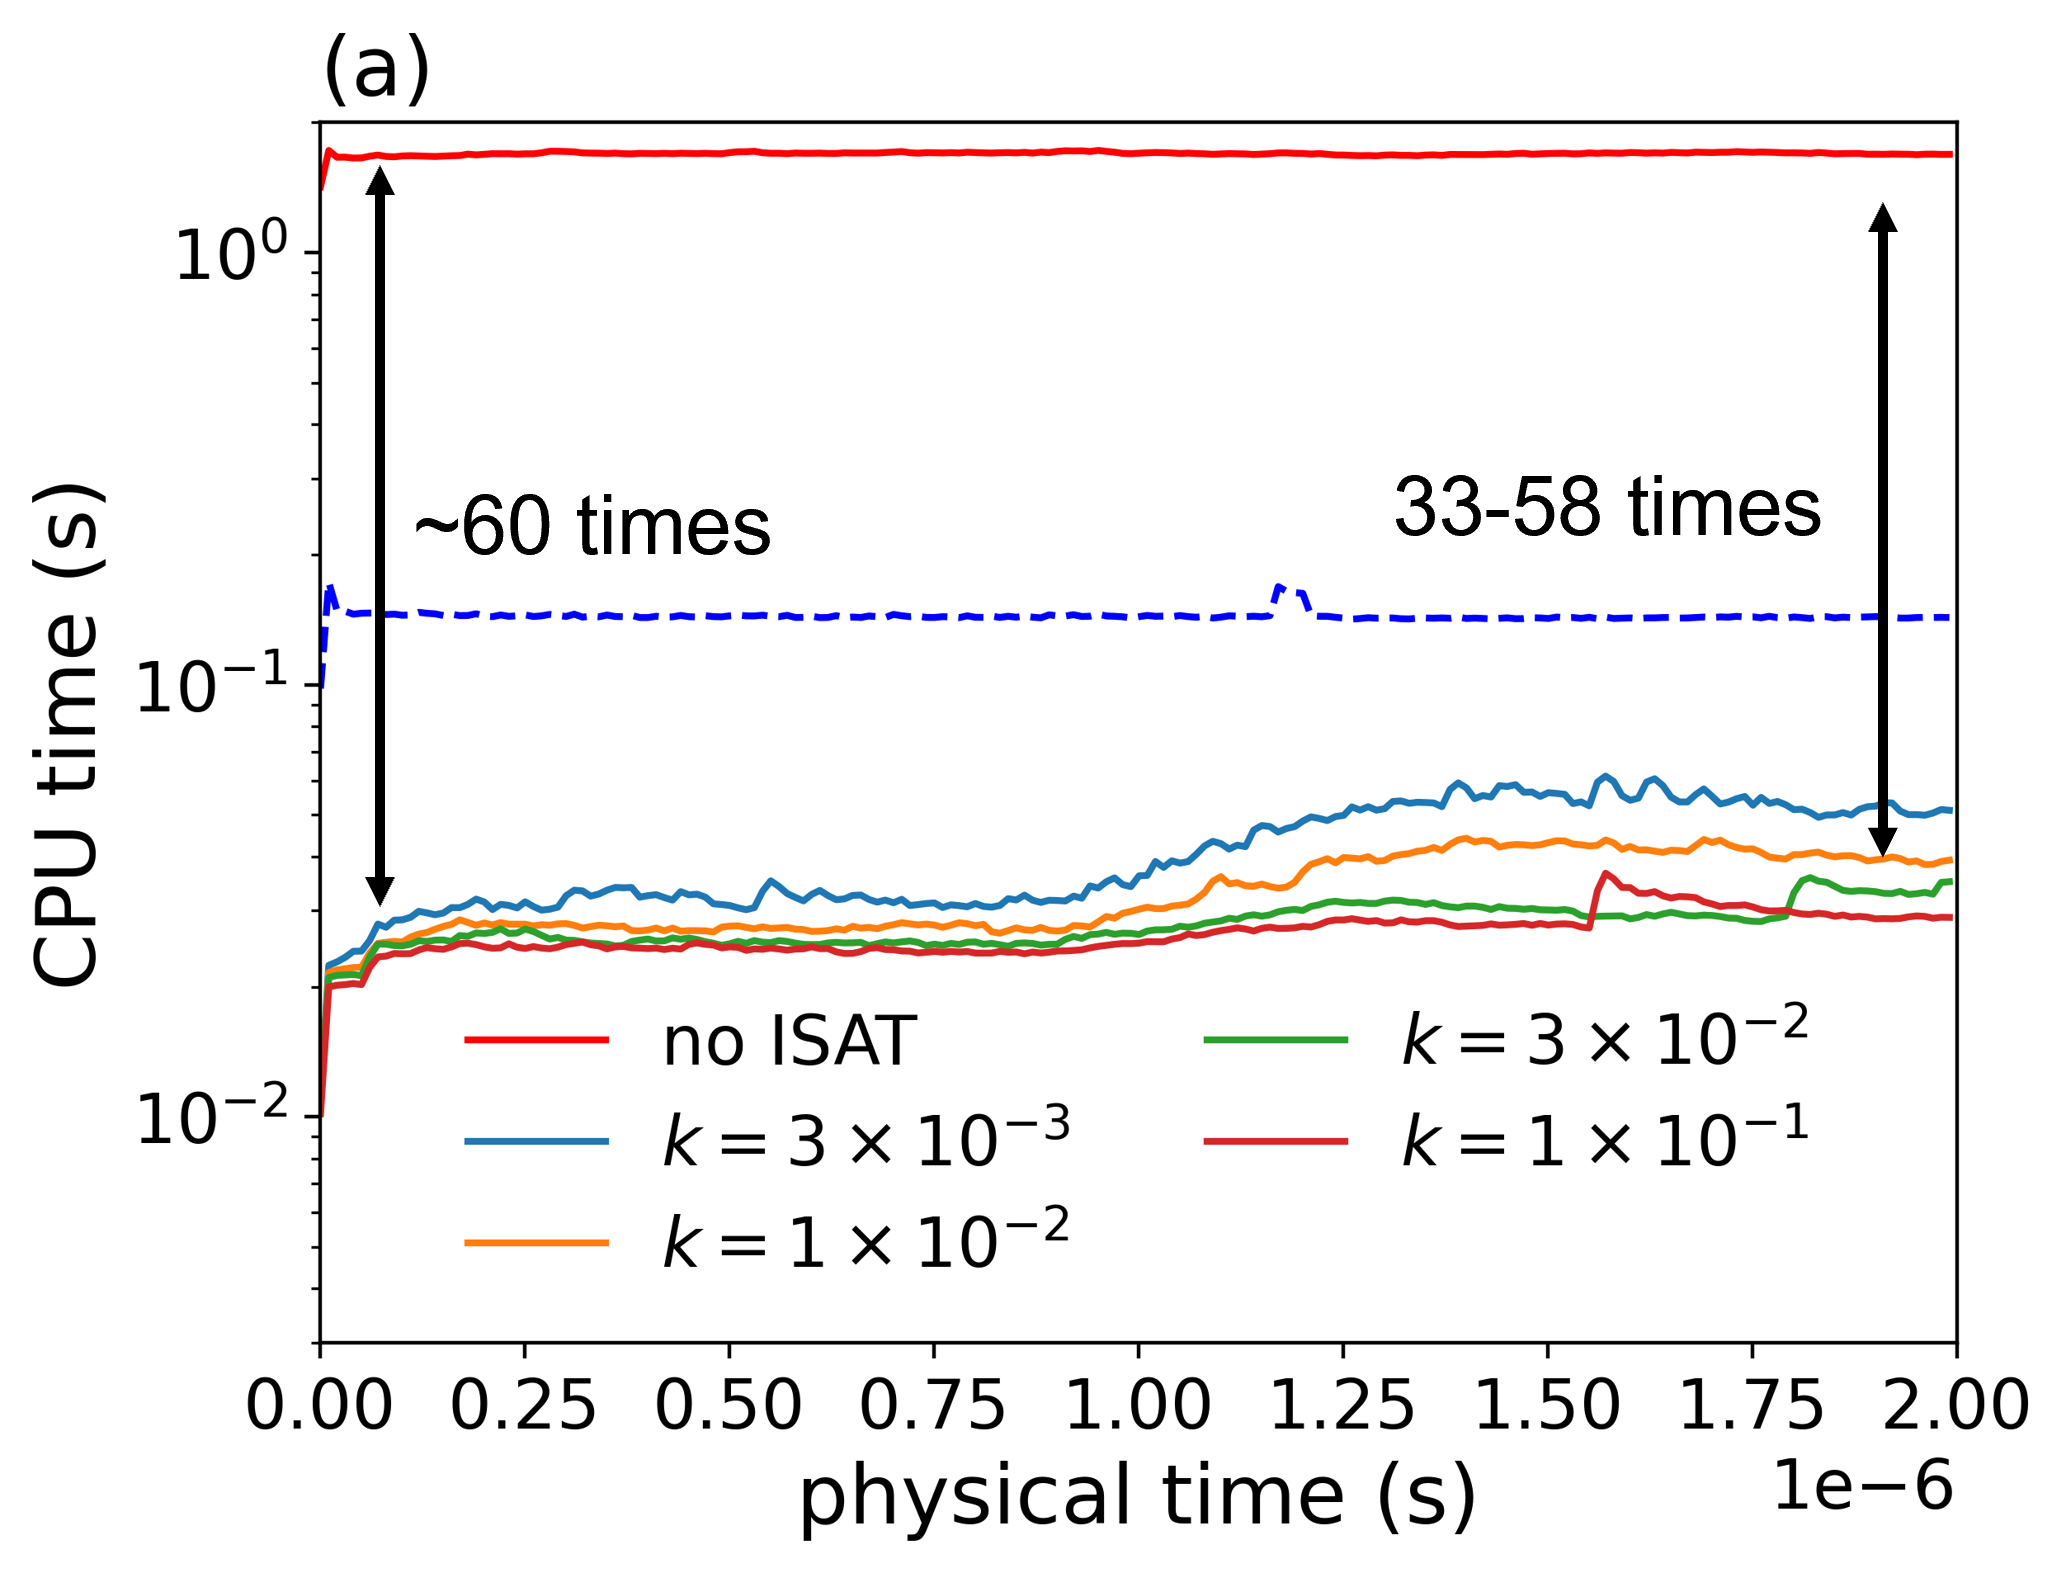
\includegraphics[width=0.45\linewidth]{time_droplet_D_2d_2_p.png}
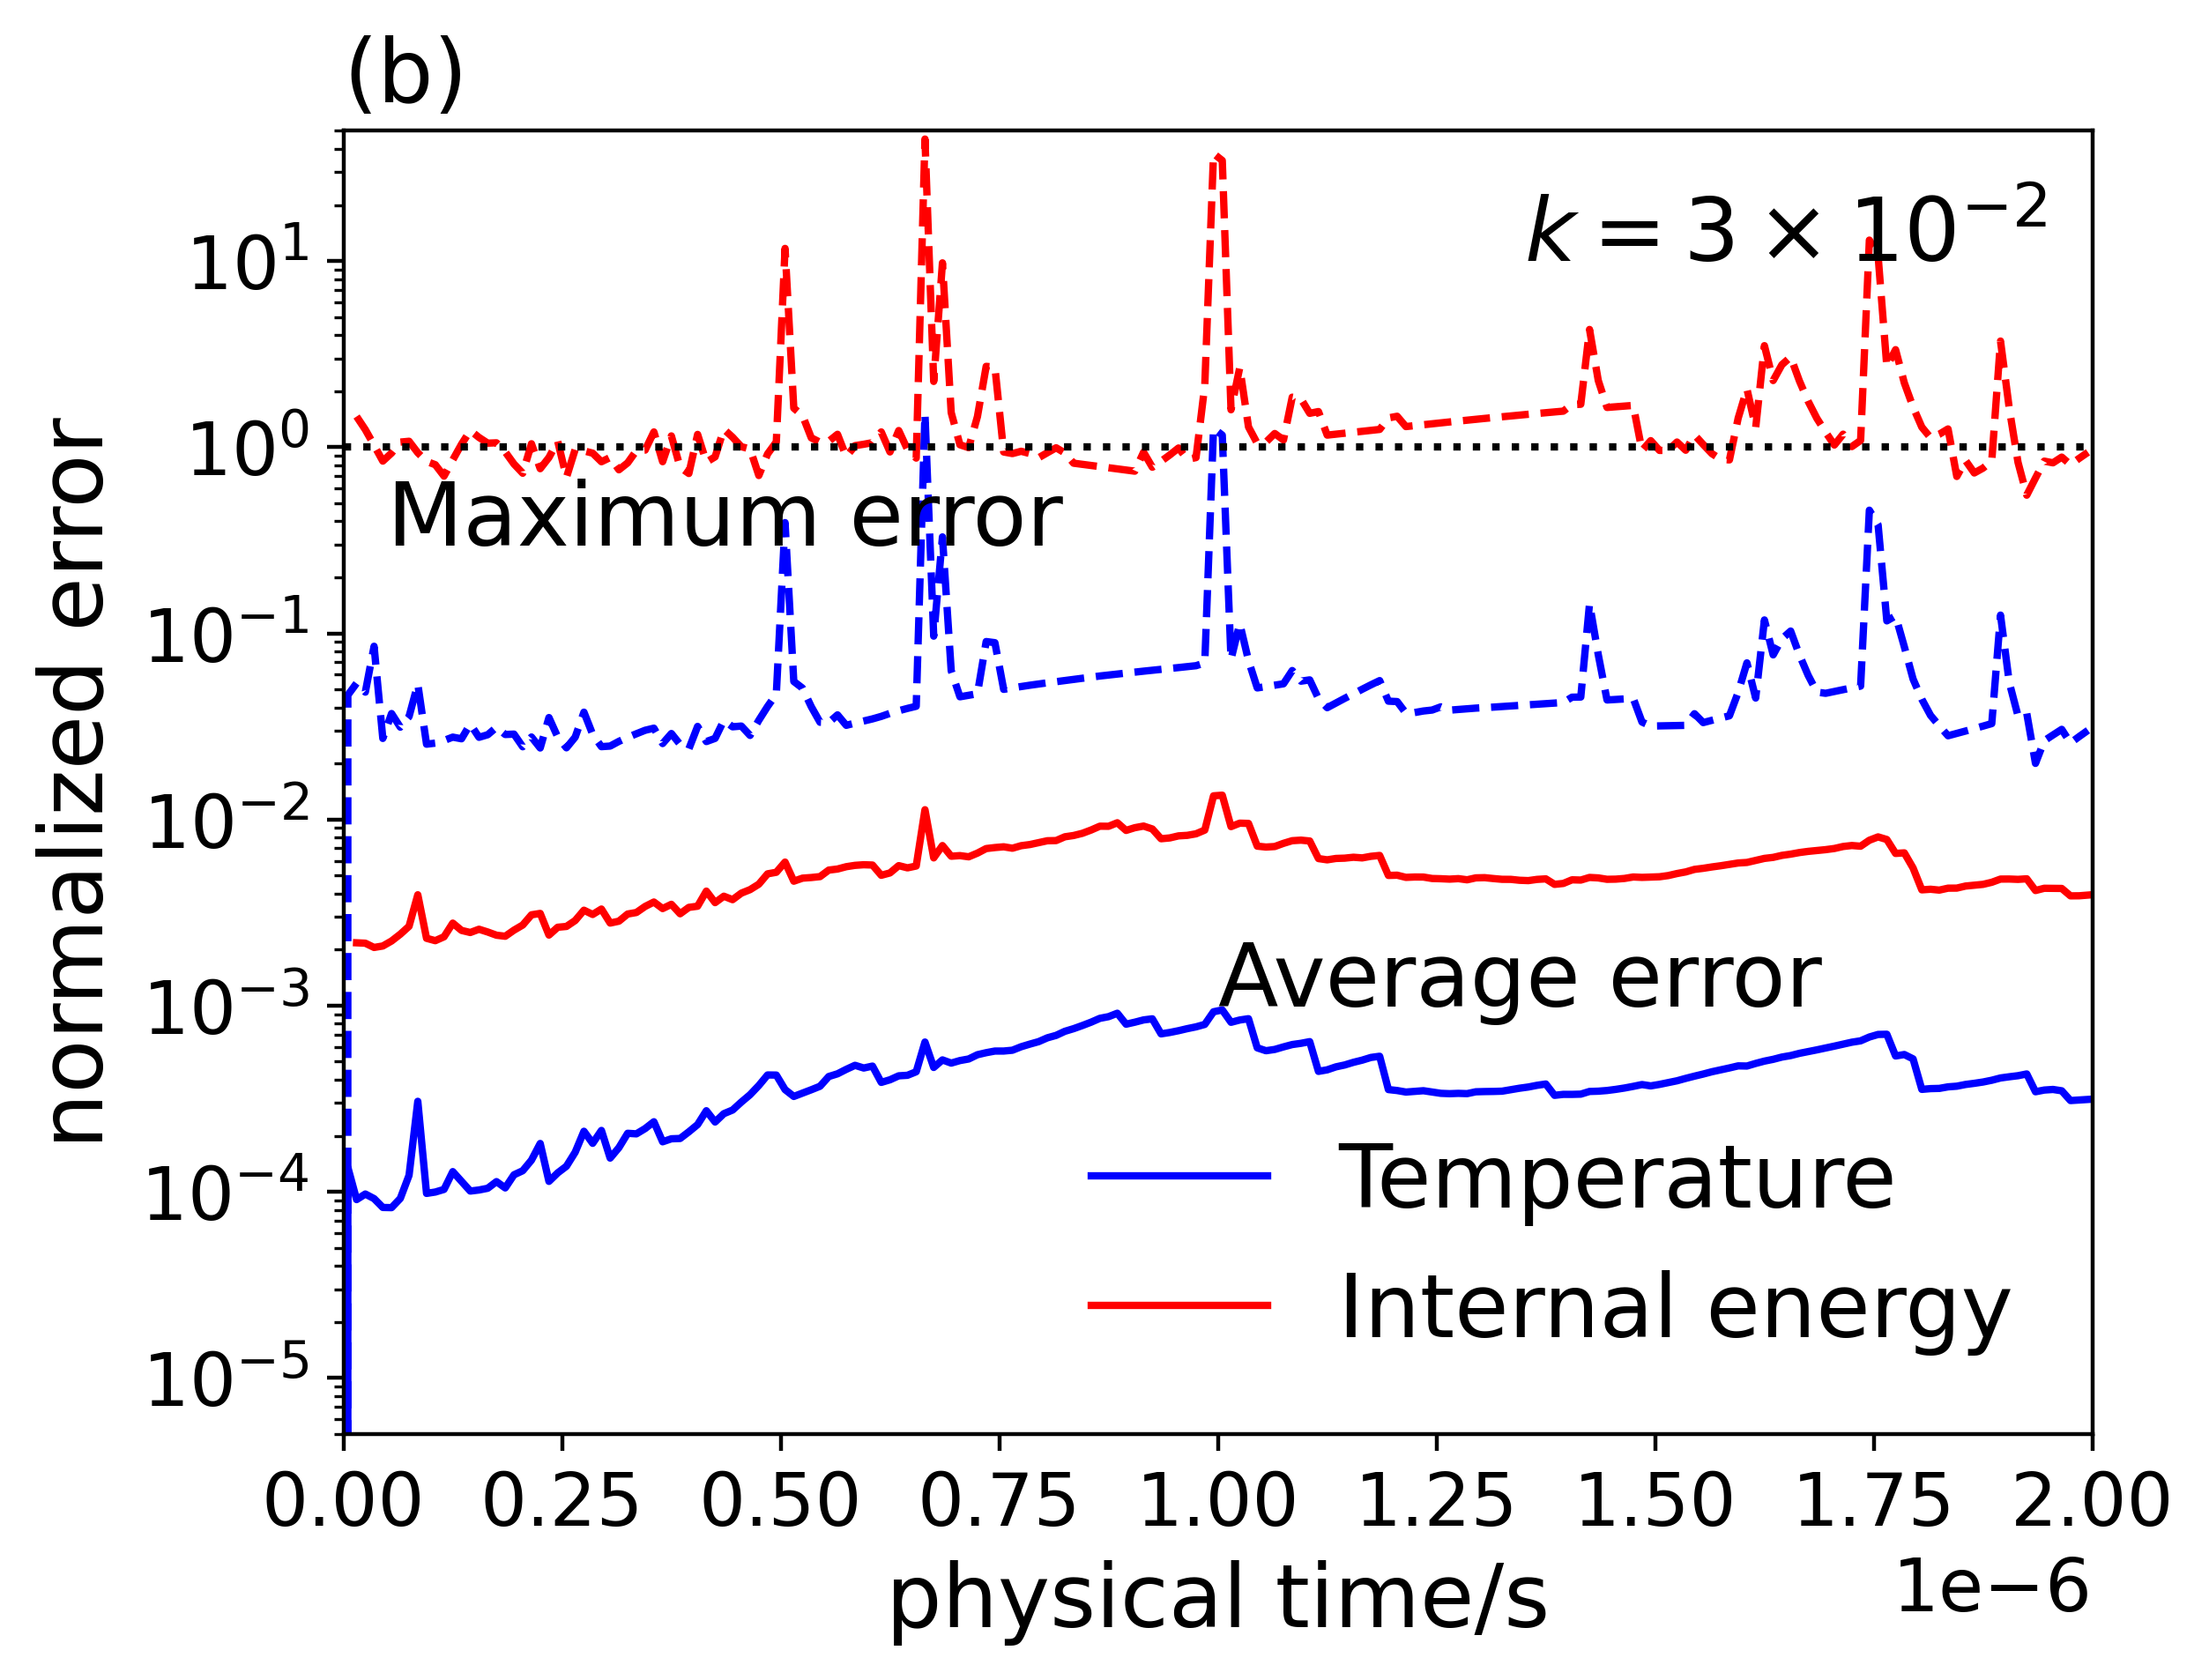
\includegraphics[width=0.45\linewidth]{error_droplet_D_2d_2.png}
\caption{(a) Performance of the ISAT-VLE method in the transcritical shock-droplet interaction simulation using the double flux (DF) scheme: the blue dotted line is the CPU time of all other parts of CFD solver, except the VLE model; the red line is the CPU time of VLE model without ISAT, and 4 lines of ISAT-VLE model with different tolerances ($k$) are provided. (b) The normalized error of the ISAT-VLE method with an error control of $k = 3 \times 10^{-2}$.}
\label{droplet_PE_D} 
\end{figure}

To mitigate the spurious oscillation resulting from real fluid effects, quasi-conservative methods are commonly employed to suppress or eliminate these oscillations. One popular approach among them is the DF method. However, it is important to note that these methods come at the cost of breaking the energy conservation law. In Fig.~\ref{droplet_DC_compare}, a comparison is made between the DF and the FC results in terms of pressure and temperature along the centerline in the x direction. This comparison is conducted when the shock wave has not yet reached the droplet position, allowing for separate analysis of the effects of the two methods on the shock wave and droplet. Without the DF method, the real fluid effect generates pressure and temperature oscillations at the droplet interface. On the other hand, the DF method successfully eliminates pressure oscillations at the droplet interface, which is the intended goal of this scheme's design. However, in order to achieve this, energy is added/removed to the discontinuity, resulting in larger temperature oscillations at the droplet interface. Additionally, breaking the energy conservation law introduces larger oscillations at the shock wave front. While some researchers argue that the energy introduced by the DF method decreases as the mesh is refined, it is often impractical to use a fine enough mesh to solve the droplet interface for 2D or 3D simulations. Therefore, breaking the energy conservation law is not considered an optimal solution. 

When the pressure oscillation in the simulation is substantial enough to cause the solution to diverge, it is preferable to allow for larger temperature oscillations while eliminating pressure oscillations. On the other hand, in simulations where temperature does not play a crucial role, the DF scheme can also be a suitable option. Conversely, when the simulation results are highly sensitive to temperature, the FC scheme is a better choice. This is precisely why we predominantly utilize the FC methods in our simulations, as the VLE process is particularly sensitive to temperature at the interface.



\begin{figure}[htbp]
\centering
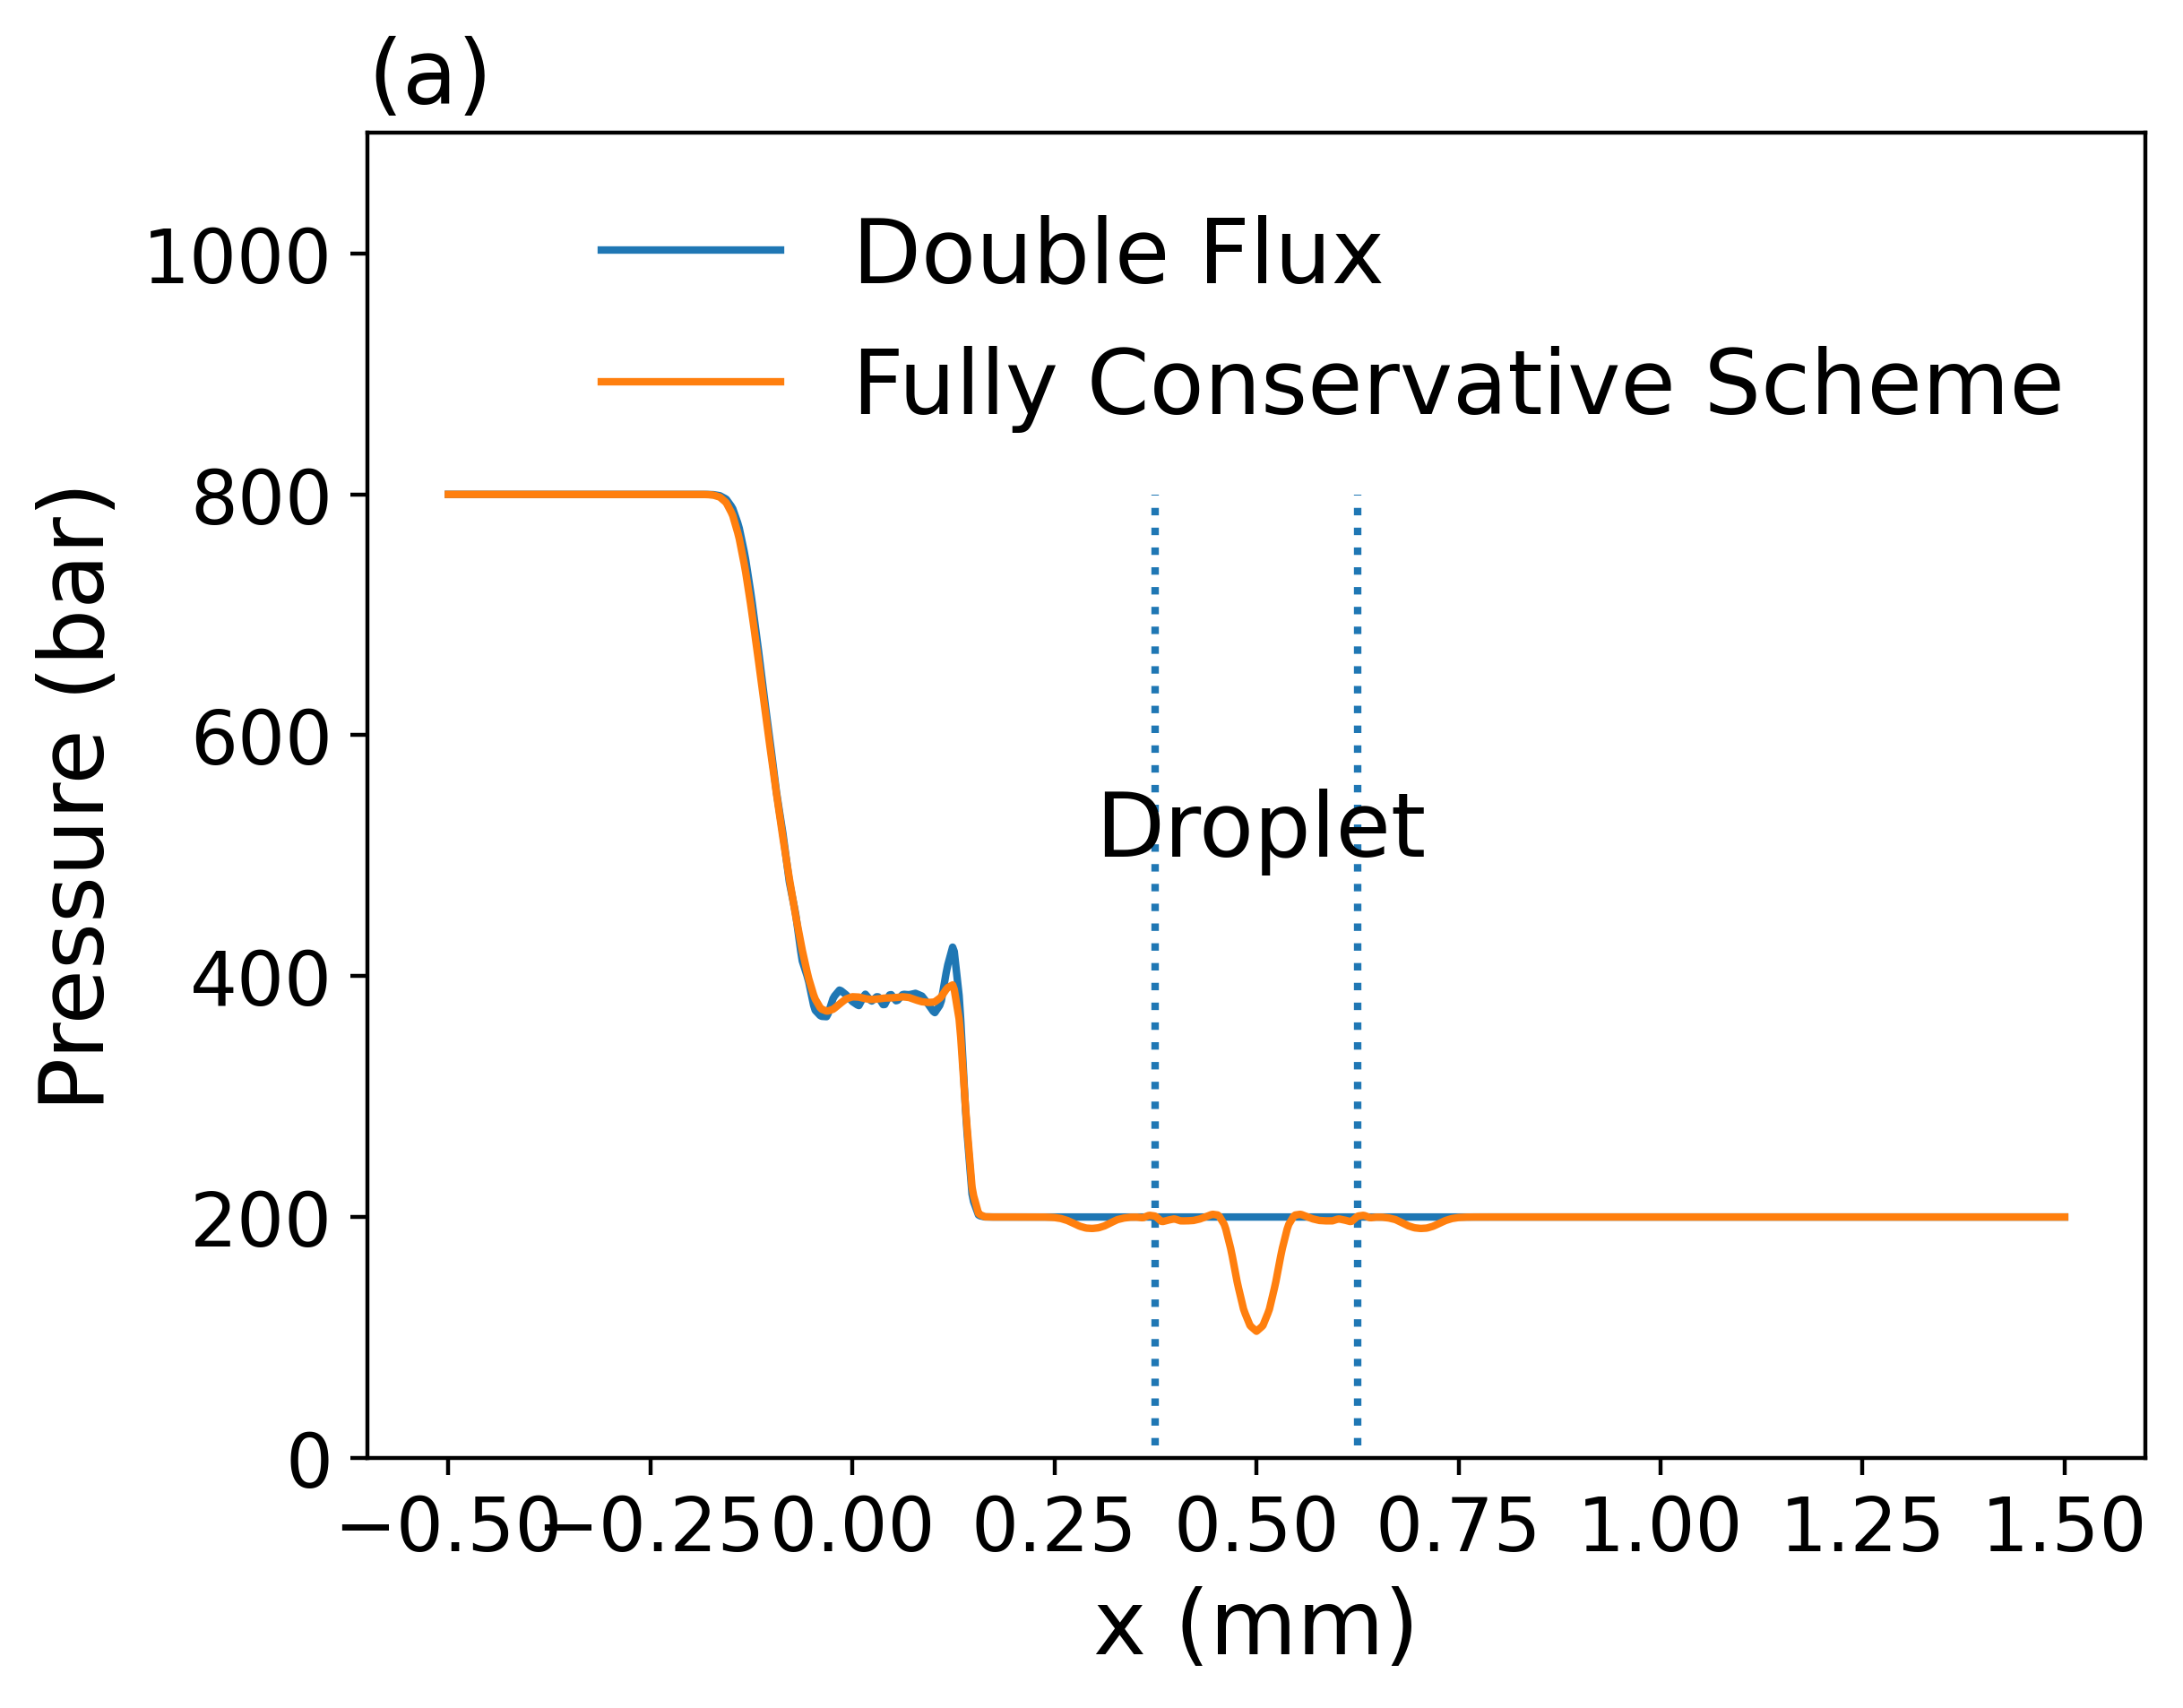
\includegraphics[width=0.4\linewidth]{DC_compare_2e_7_p.png}
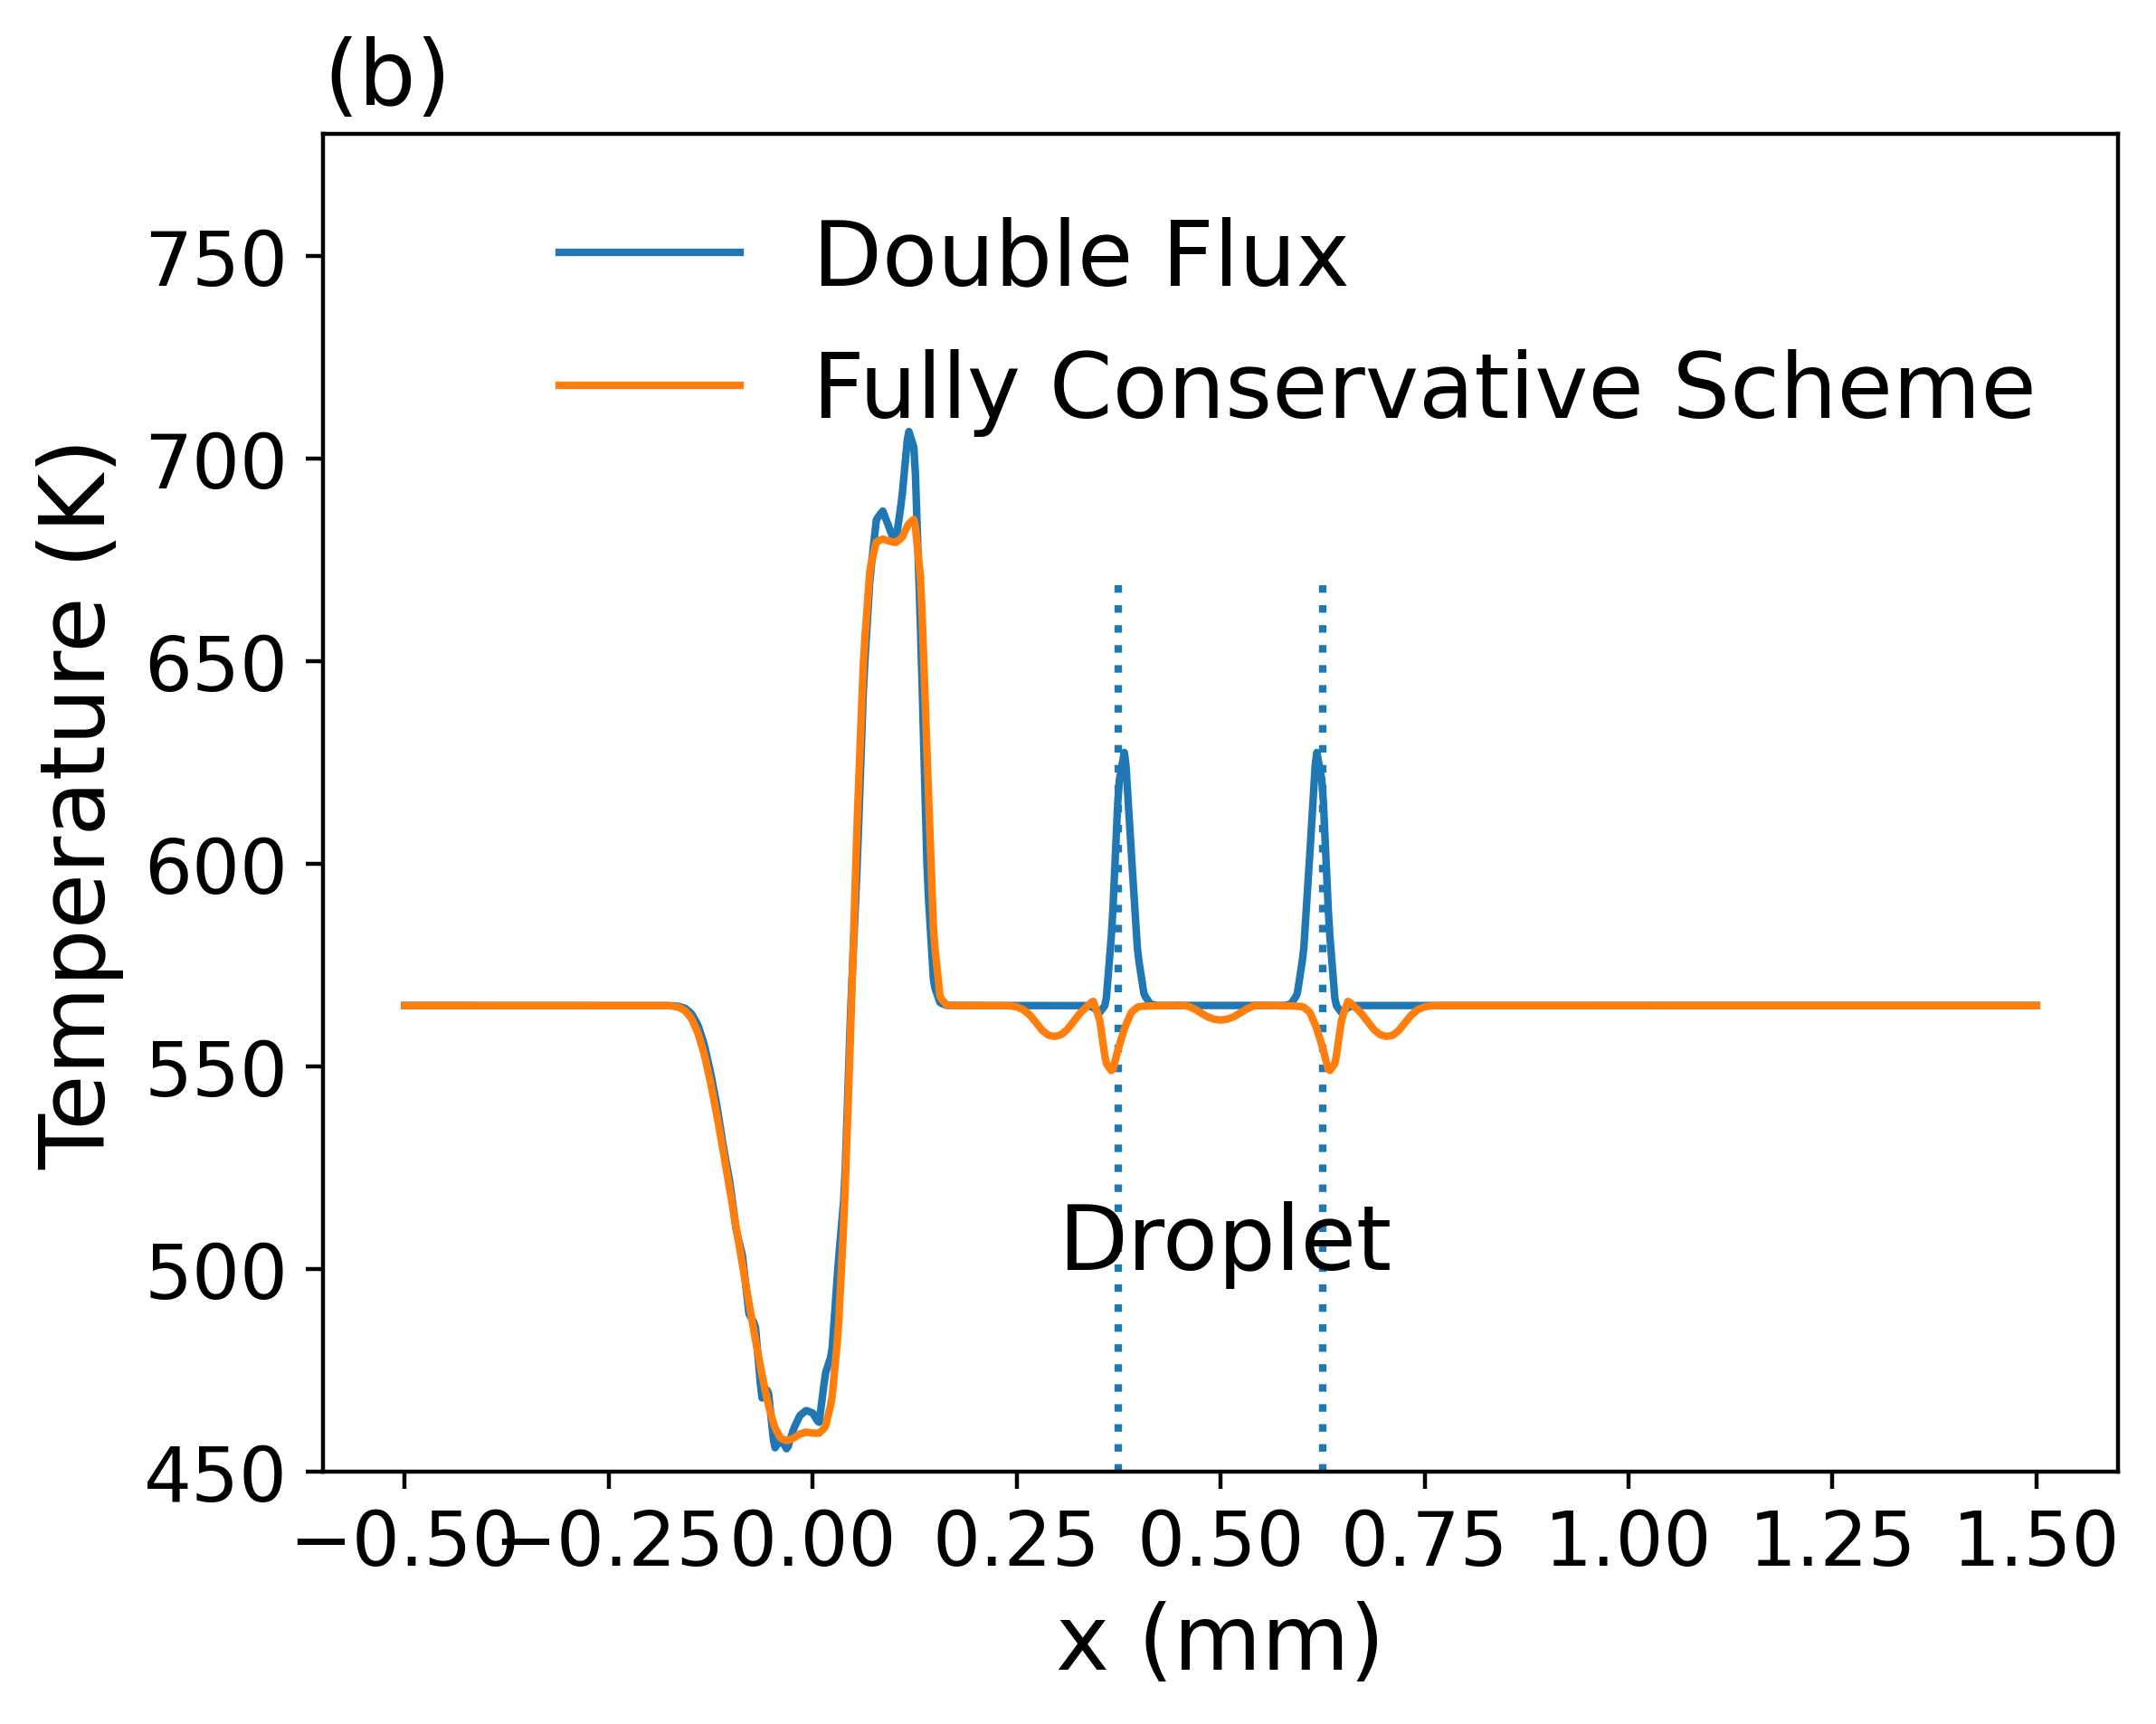
\includegraphics[width=0.4\linewidth]{DC_compare_2e_7_T.png}
\caption{Comparison between fully conservative (FC) scheme and double flux (DF) method results: (a) pressure, and (b) temperature. The results show the properties at the horizontal center line along $x$ direction through the droplet center.}
\label{droplet_DC_compare} 
\end{figure}

\subsubsection{Redundant records deletion methods}
\label{sec:delete}
In Sec.\ref{sec:ISAT}, we introduced new methods for deleting redundant records, and in this subsection, we assess their performance through shock-droplet interaction simulations using the FC scheme. Sec.\ref{sec:ISAT} illustrates the test results. First, we examined the outcomes without active data removal (FS: fixed maximum table size). Three different maximum table sizes were employed (FS1: 140,000, FS2: 130,000, FS3: 120,000). It can be observed that the FS3 result is slower compared to FS1 and FS2. This is because the maximum table size in FS3 is insufficient to store an adequate number of records , leading to more VLE problem-solving and thus reducing performance. Once the table size is adequately large, further increasing the maximum size no longer significantly impacts performance. Hence, the results for FS1 and FS2 are close to the limits of this method.

Next, we conducted separate tests for our proposed methods: the maximum unused step method (MUS) and the adaptive maximum table size method (AS). In MUS, we actively eliminate data that hasn't been used within the last 80 time steps. In AS, we utilized parameters $C = 5.8$ and $M = 5$ to update the maximum table size (Eq.\ref{eq:adap}). Both methods resulted in reduced CPU time and achieved approximately a 4\% performance improvement. When both methods were used concurrently (AS+MUS), the performance was further enhanced by approximately 2\%. It is worth noting that the ISAT method has already undergone substantial optimization, effectively utilizing computational resources. However, we identified additional optimization opportunities, and our methods still yielded a 6\% performance improvement. This AS+MUS method was employed for all simulations in this study.


\begin{figure}[htbp]
\centering
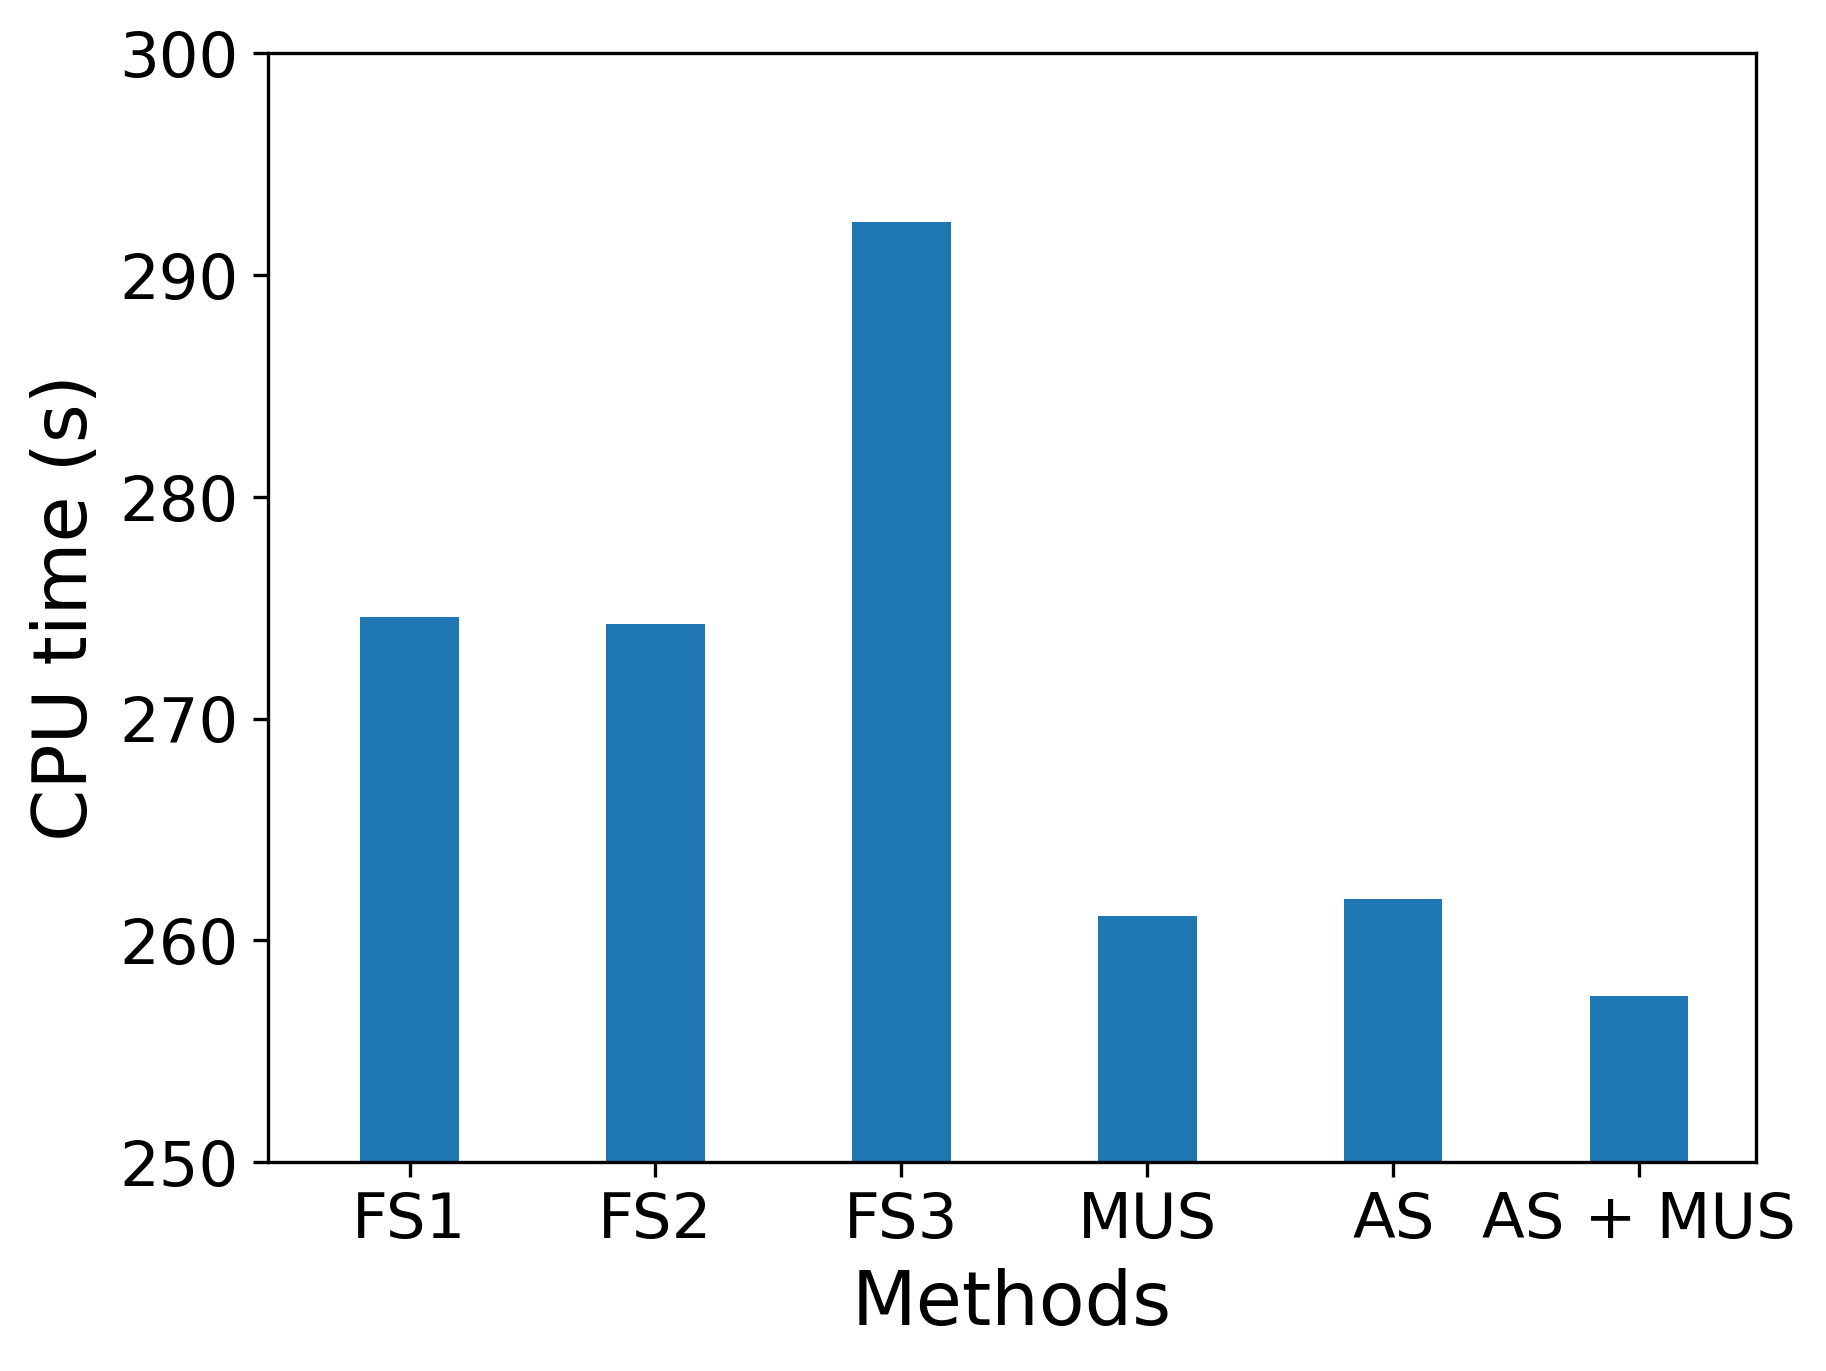
\includegraphics[width=0.45\linewidth]{llist.png}
\caption{Comparison between redundant records deletion methods. The fixed maximum table size method (FS) only removes data when the table is full, and the least recently used record is removed. The maximum table sizes for the 3 settings are, FS1: 140000, FS2: 130000, and FS3:120000. The maximum unused step method (MUS), removes records that haven't been used for a given number of time steps. 80 time steps are used for MUS. The adaptive maximum table size method (AS) used Eq.~\ref{eq:adap} to determine maximum table size, and $C=5.8, M=5$}
\label{droplet_delete} 
\end{figure}

%mutli conponent speed (TODO)

%\textbf{parallel simulation}
\subsubsection{Shock-droplet interaction in 3D simulations}
\label{sec:SD_3D}

In this subsection, we performed a series of 3D transcritical shock-droplet interaction simulations using the FC scheme. A grid convergence study is conducted, and results are shown in Appendix~\ref{App:SD}.Fig.~\ref{droplet_3d_1C} displays the 3D results at three different time instances: $5\times 10^{-7}$ s, $8.3\times 10^{-7}$ s, and $1.2\times 10^{-6}$ s, illustrating the propagation of the shock wave passing through the droplet. The results show the reflection wave and the deformation of the droplet induced by the shock wave. To gain a better understanding of the phase change, the thermodynamic state is plotted in the pressure-temperature (P-T) phase diagram (Fig.~\ref{droplet_3D_1C_phasediagram}). Since our focus is solely on the shock wave front and the interaction between the shock and droplet, data points corresponding to the expansion wave are excluded. In Fig.~\ref{droplet_3D_1C_phasediagram}, all data points can be clearly categorized into two distinct parts. The first part consists of points forming a curve in the lower right region, which represents the shock front connecting the pre-shock and post-shock ambient conditions. The second part comprises the remaining points, forming a band that corresponds to the droplet. This is attributed to the influence of \ce{n-C12H26}, causing the post-shock condition of the droplet to have lower pressure and temperature compared to the ambient post-shock condition. For the droplet points, the pressure undergoes a dramatic increase due to the shock wave, while the temperature remains relatively unchanged. A significant portion of these data points falls within the two-phase region (indicated by high $\alpha$ values), which requires VLE modeling. Moreover, despite the working pressure (350 bar - 400 bar) being much higher than the critical pressure of pure \ce{n-C12H26} (18 bar), the multi-component effect yields very high mixture critical pressures (560 bar at $x_N2 = 0.85$). As a result, the thermodynamic state is pushed back to the subcritical two-phase region (as depicted in Fig.~\ref{droplet_3D_1C_phasediagram}), leading to phase separation (as observed in Fig.~\ref{droplet_3d_1C}).

\begin{figure}[htbp]
\centering
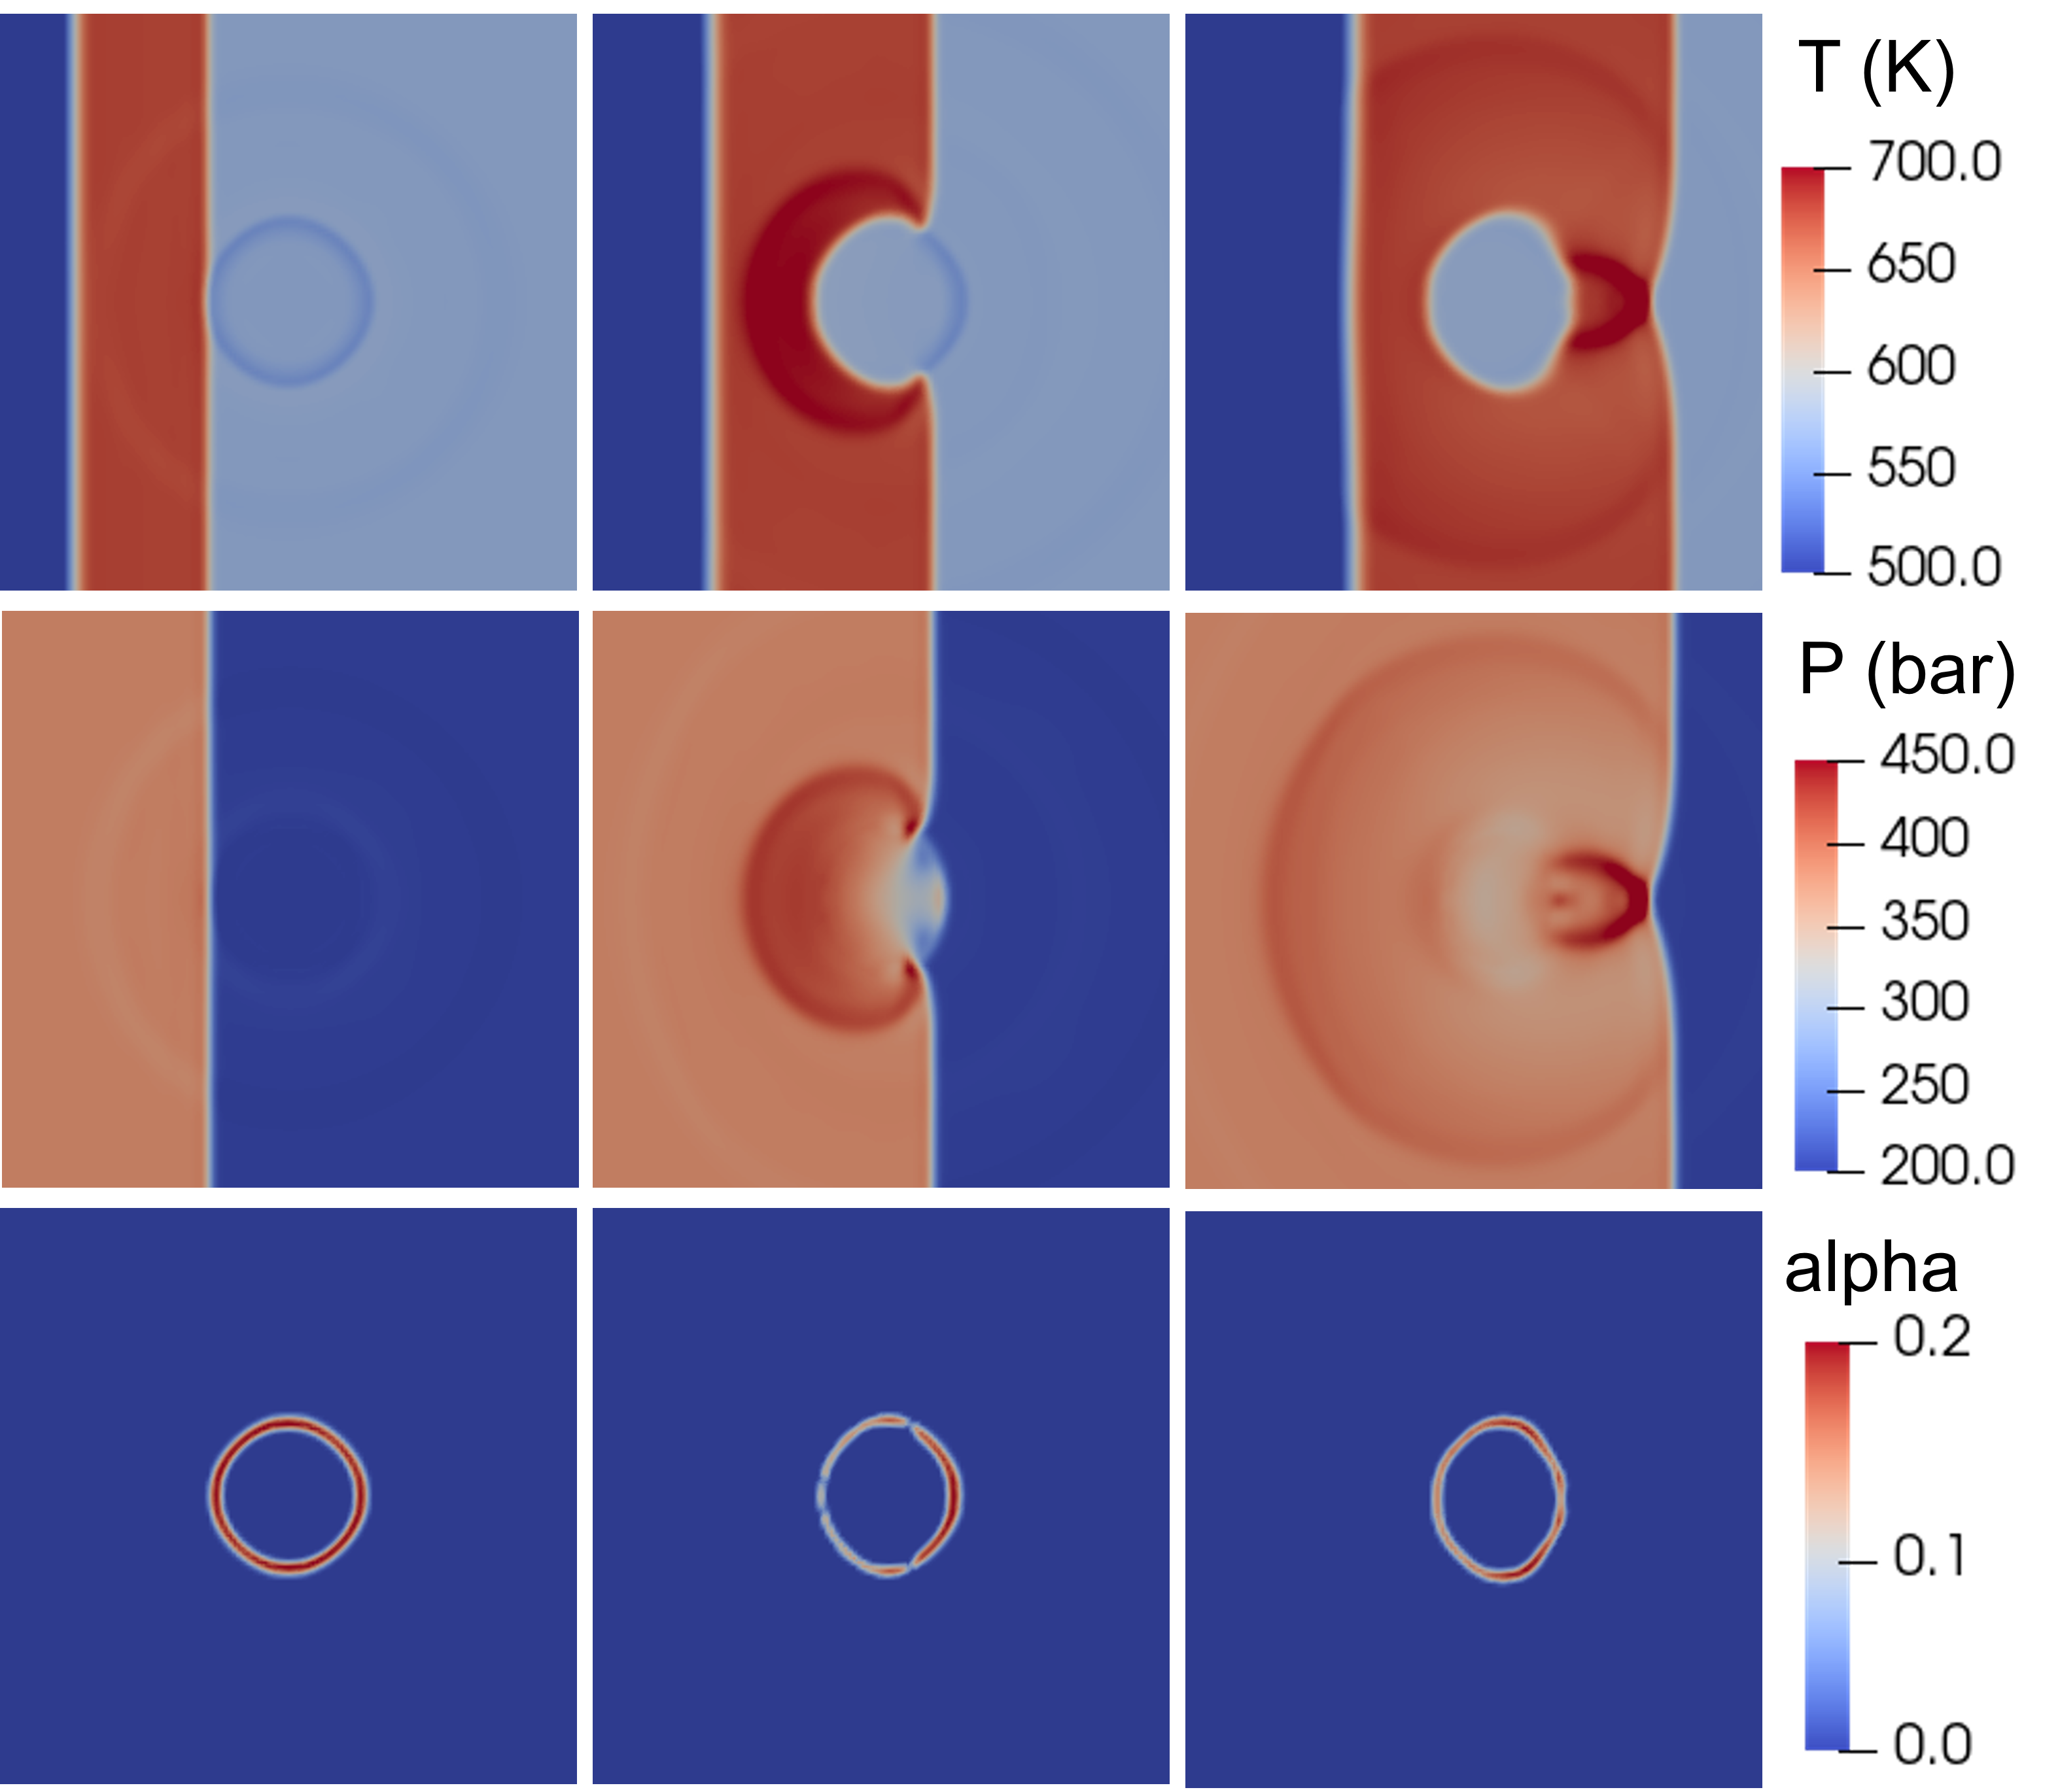
\includegraphics[width=0.65\linewidth]{3D_shock_1C_2.png}
\caption{Transcritical shock-droplet interaction simulation with an initial temperature of 565 K: the top figures are density, and the bottom figures are $\alpha$, where $\alpha = \beta (1-\beta)$ is a two-phase interface indicator. From left to right are the time instants of $5\times 10^{-7}$ s, $8.3\times 10^{-7}$ s, and $1.2\times 10^{-6}$ s. }
\label{droplet_3d_1C} 
\end{figure}

\begin{figure}[htbp]
\centering
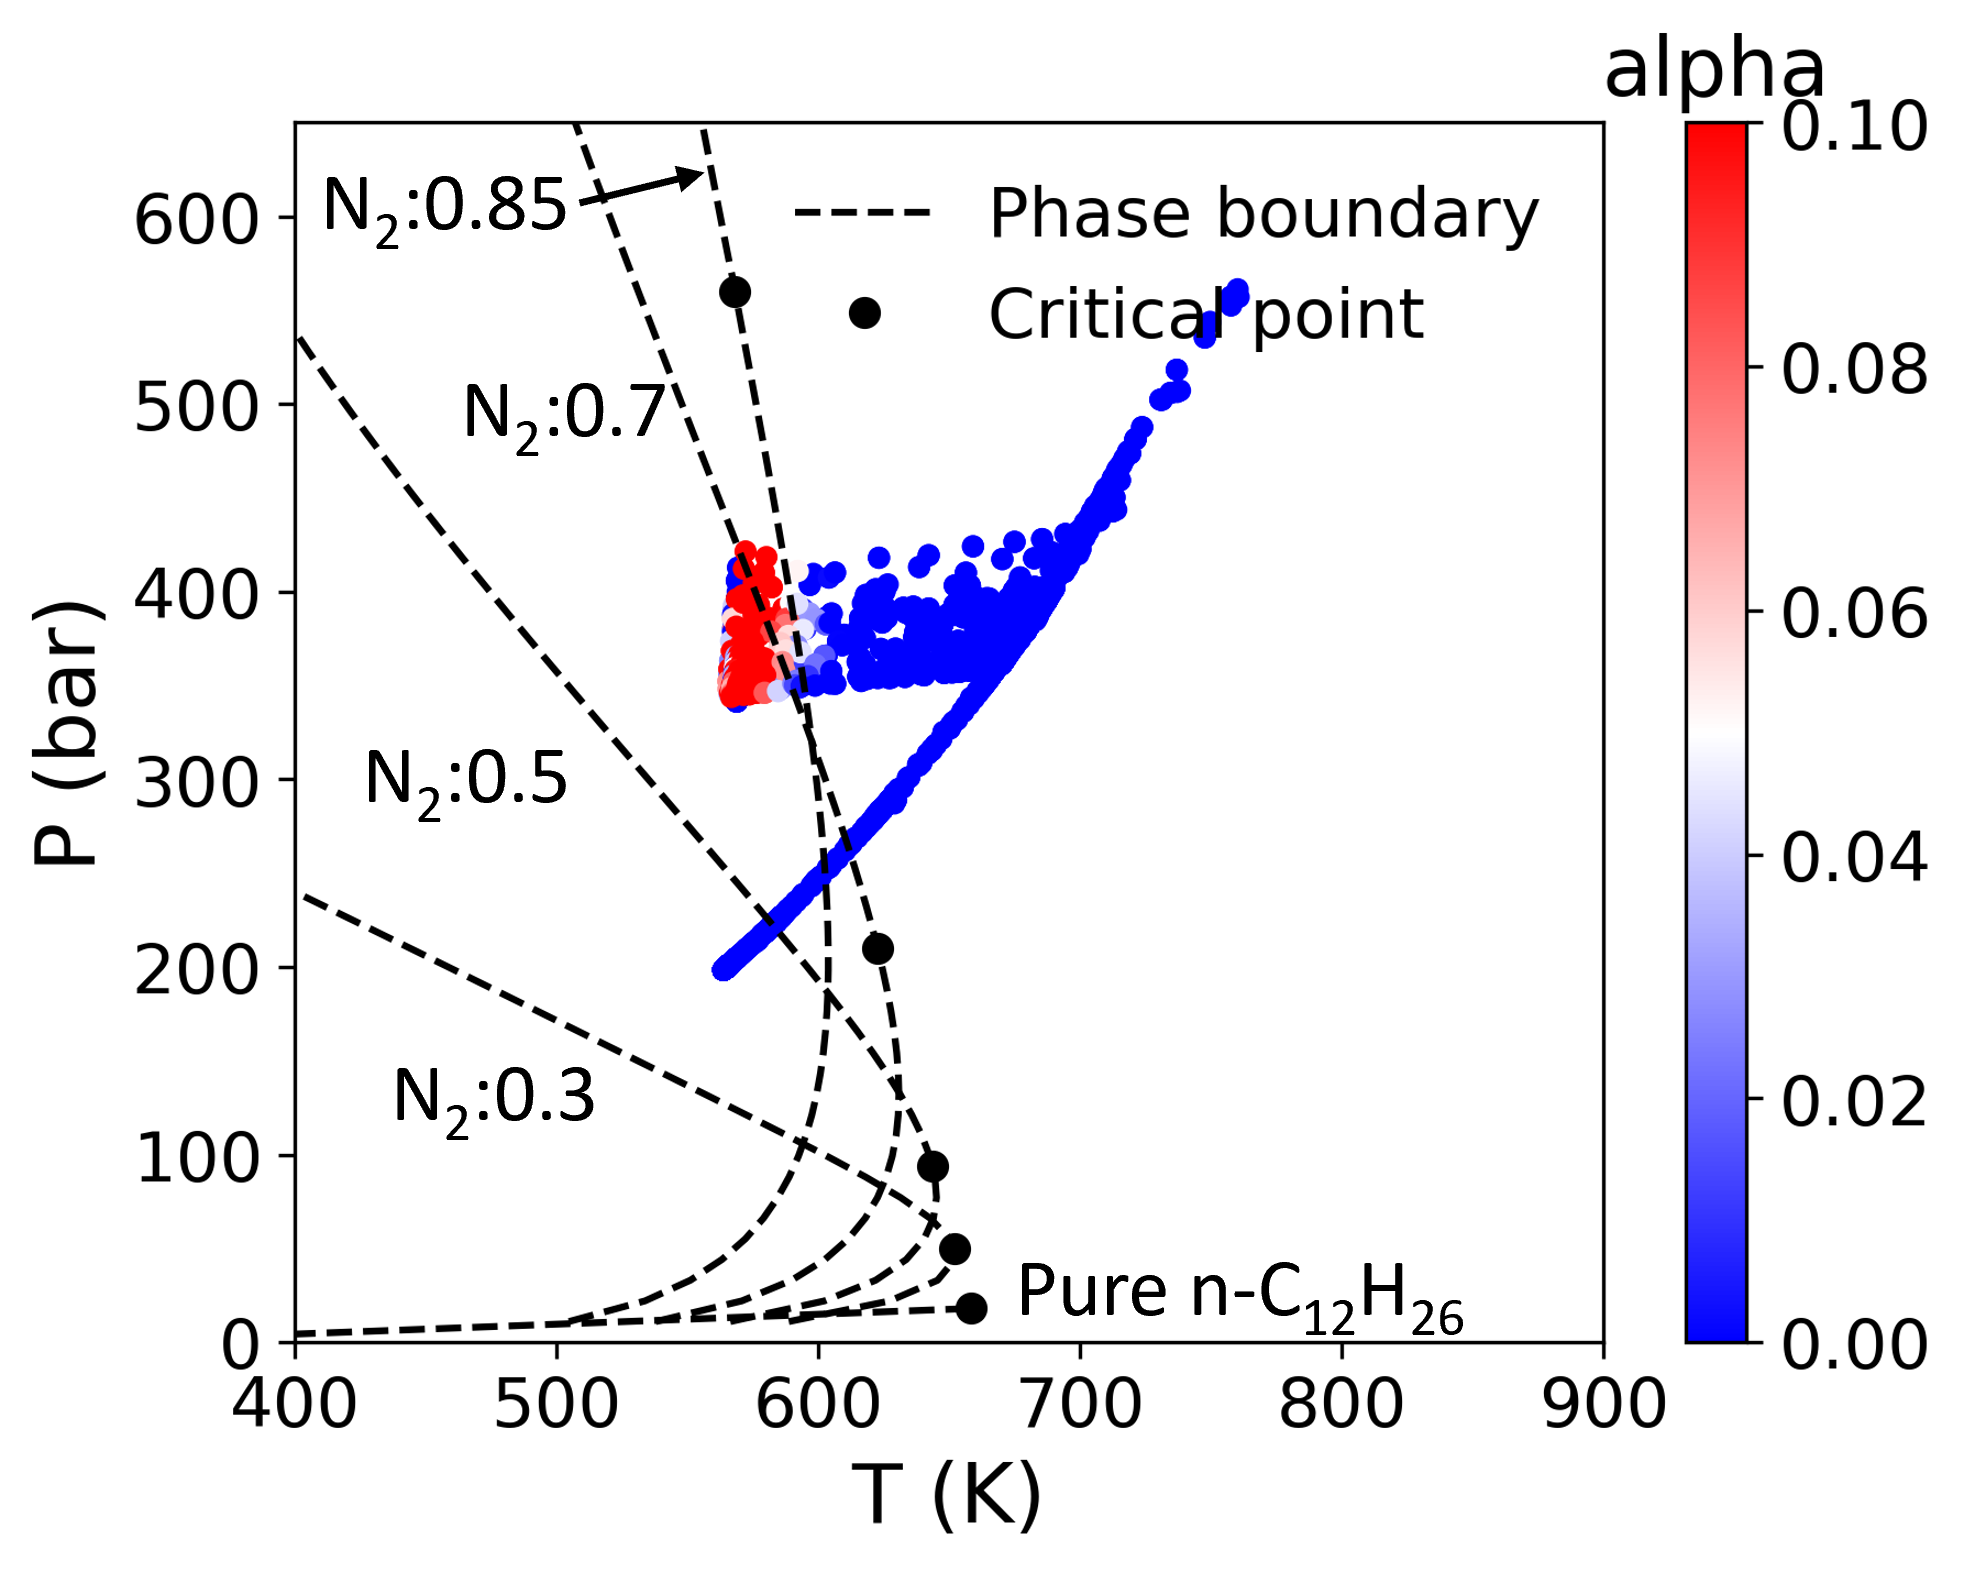
\includegraphics[width=0.50\linewidth]{PT_1C_2_p.png}
\caption{Phase diagram of the transcritical shock-droplet interaction simulation with an initial temperature 565 K. The label is the mole fraction of \ce{N2}. The data points are taken from the time instance of $1.2\times 10^{-6}$ s. The data points of the expansion wave are removed}
\label{droplet_3D_1C_phasediagram} 
\end{figure}

Fig.~\ref{SD_3D_err} illustrates the evolution of temperature and pressure errors in the 3D shock-droplet interaction simulation. It can be observed that these errors primarily manifest at the shock front and the acoustic waves generated by spurious oscillations. A notable distinction between the temperature and pressure errors is that the temperature error remains localized to the surface of the droplet, whereas the pressure error extends into the droplet's interior. This discrepancy arises due to the minimal influence of the shock wave on the droplet's temperature during its passage (as shown in Fig.~\ref{droplet_3d_1C}). Although the acoustic wave propagates the errors of both temperature and pressure over a wider region, their magnitudes are well-controlled. The temperature error is less than 0.1 K, and the pressure error remains below 0.2 bar. Both relative errors are maintained below 0.1\%. Consequently, the ISAT method demonstrates excellent error control in the 3D simulations.



\begin{figure}[htbp]
\centering
\includegraphics[width=0.65\linewidth]{3D_shock_1C_err_2.png}
\caption{The error contours of ISAT-VLE method in the 3D transcritical shock-droplet interaction simulation. From left to right are the time instants of $5\times 10^{-7}$ s, $8.3\times 10^{-7}$ s, $120\times 10^{-7}$ s. The labels in the figure are mole fractions.}
\label{SD_3D_err} 
\end{figure}

If the initial temperature is increased to 620 K, it significantly affects the phase separation effect at the interface. Initially, as shown in Fig.~\ref{droplet_3d_1C_HT}, the two-phase indicator $\alpha$ indicates that the droplet interface is situated within the subcritical two-phase region. However, as the shock wave passes through the droplet, the interface transitions into the single-phase region, eventually leading to the complete disappearance of the phase separation effect. This process is further illustrated in the phase diagram depicted in Fig.~\ref{droplet_3D_1C_HT_phasediagram}. The data points of the initial condition lie within the phase boundary of the mixture with $x_{N2}=0.7, x_{C12H26}=0.3$, confirming that the droplet interface exists in the subcritical two-phase region. As the shock wave elevates the droplet's pressure, the thermodynamic conditions move outside of the phase boundary, resulting in the elimination of phase separation. 

In this work, we did not include the modeling of surface tension. However, based on our findings, we anticipate that under these conditions, the mechanism of droplet break-up would be governed by surface tension prior to the shock wave, and subsequently influenced by the diffusion effect after the shock wave, as phase separation is eliminated.




\begin{figure}[htbp]
\centering
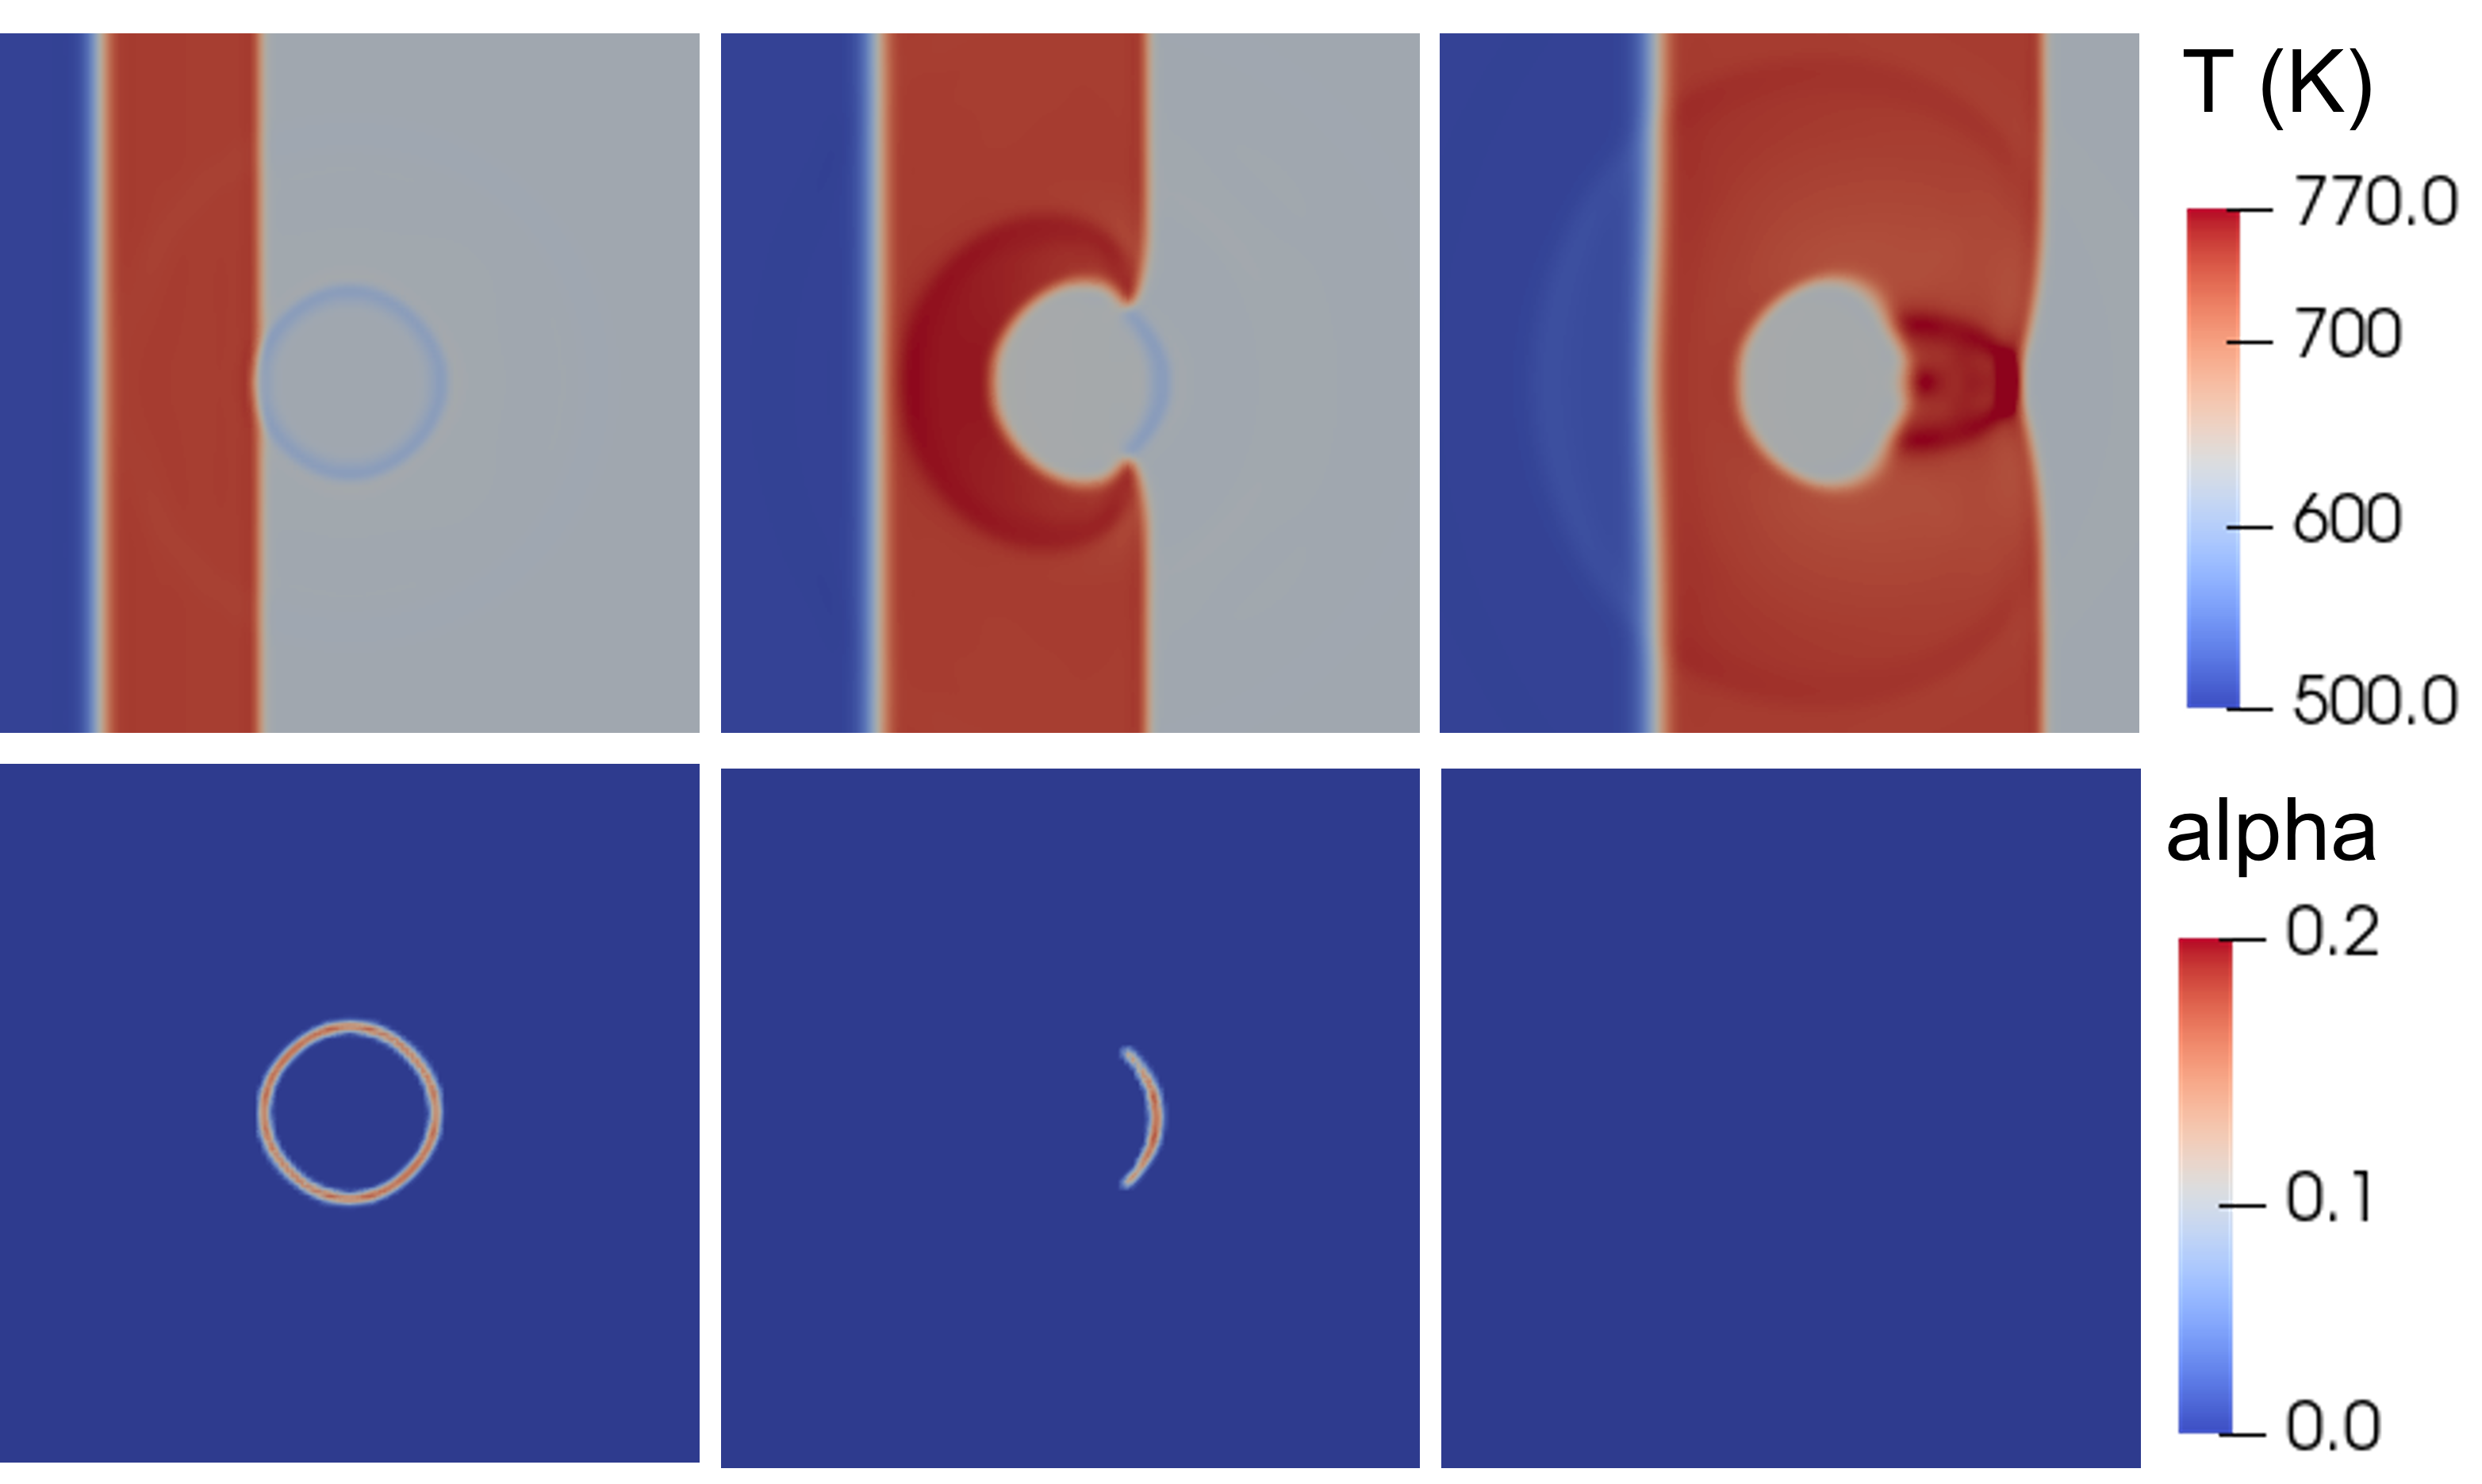
\includegraphics[width=0.65\linewidth]{3D_shock_1C_HT_3.png}
\caption{Transcritical shock-droplet interaction simulation with an initial temperature of 620 K: the top figures are density, the bottom figures are $\alpha$, where $\alpha = \beta (1-\beta)$ is a two-phase interface indicator. From left to right are the time instants of $5\times 10^{-7}$ s, $8.3\times 10^{-7}$ s, and $1.2\times 10^{-6}$ s.}
\label{droplet_3d_1C_HT} 
\end{figure}


\begin{figure}[htbp]
\centering
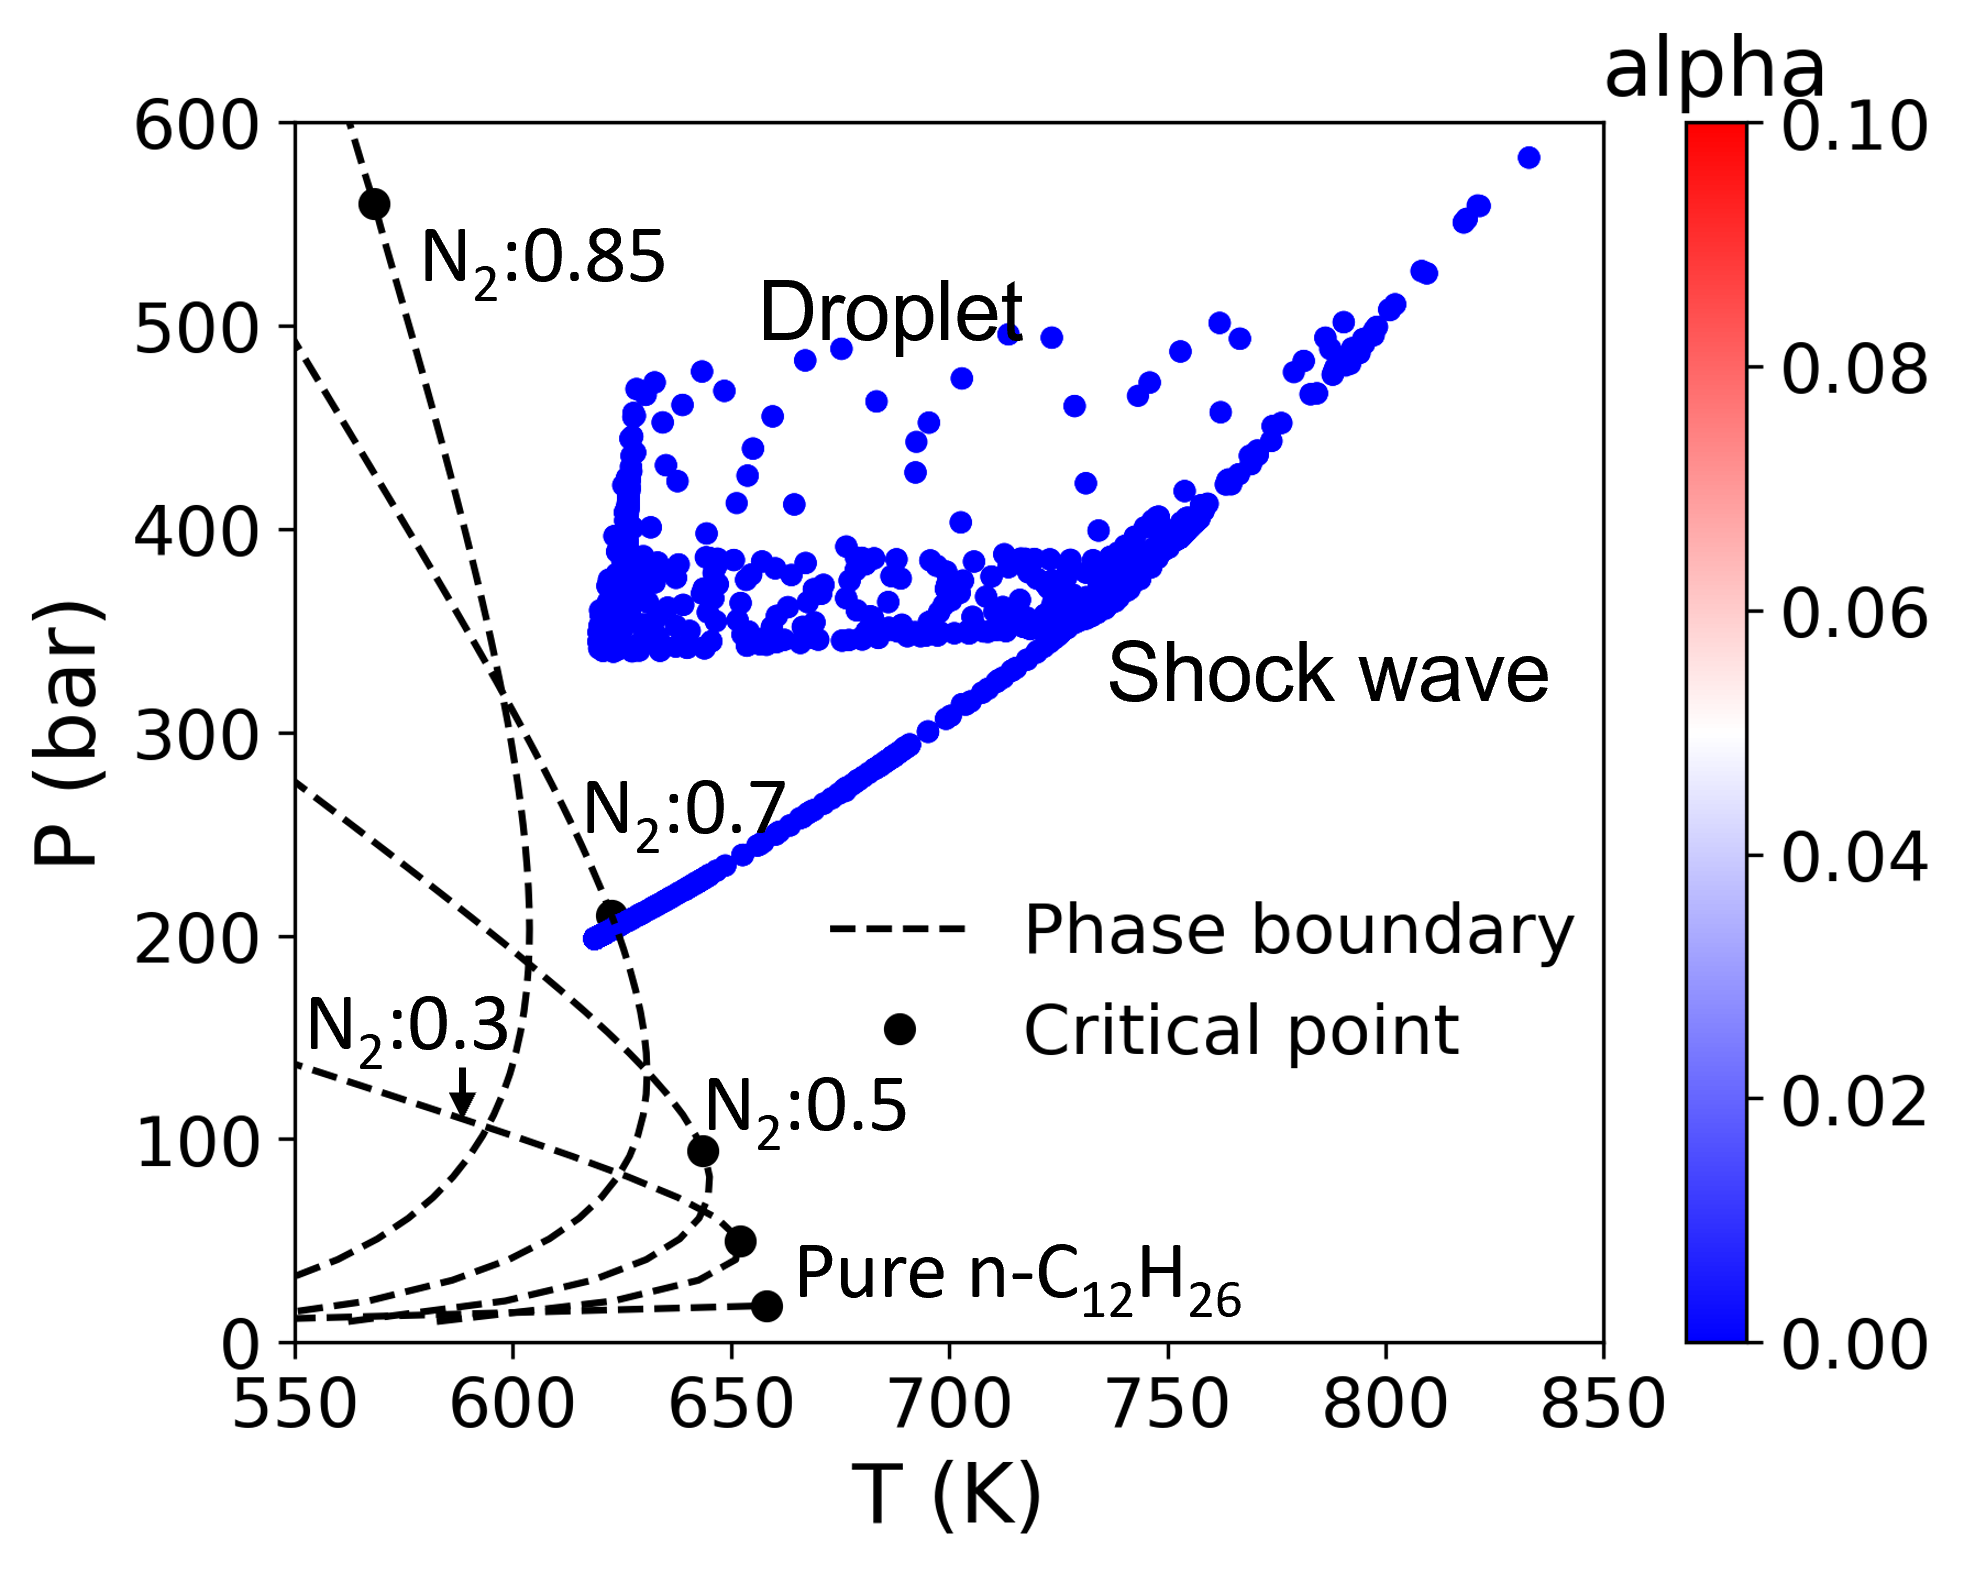
\includegraphics[width=0.50\linewidth]{PT_1C_HT_2_p.png}
\caption{Phase diagram of transcritical shock-droplet interaction simulation with an initial temperature 600K. Data points are taken from the time instance of $1.2\times 10^{-6}$ s. The labels in the figure are mole fractions.}
\label{droplet_3D_1C_HT_phasediagram} 
\end{figure}

Next, we explore the behavior of a two-component droplet. In this simulation, the droplet consists of 60\% \ce{n-C12H26} and 40\% \ce{n-C8H18} (by mole). The initial temperature is set to 565 K, which is consistent with the first case in this subsection. In Fig.~\ref{droplet_3d_2C}, as the shock wave passes through the droplet, we observe the disappearance of part of the two-phase boundary. This is because \ce{n-C8H18} has a lower critical temperature (\ce{n-C8H18} 568.9K, \ce{n-C12H26} 658.2 K) and changes the phase boundary (see in Fig.~\ref{droplet_3D_2C_phasediagram}) However, an additional phenomenon is also observed: even after the shock wave completely passes through the droplet, some sections of the droplet interface remain in the two-phase region. This is attributed to the relatively low pressure in the wake region behind the droplet, allowing the interface to remain in the subcritical two-phase region. This reasoning is clearly depicted in the phase diagram Fig.~\ref{droplet_3D_2C_phasediagram}, where the three-component system (\ce{n-C12H26}/\ce{n-C8H18}/\ce{N2}) exhibits a two-phase region overlapping with the low-pressure corner of the post-shock data points. Under such special conditions, the breakup of the droplet could be influenced by both surface effects and diffusion simultaneously, which could lead to the complex interaction of these mechanisms.





\begin{figure}[htbp]
\centering
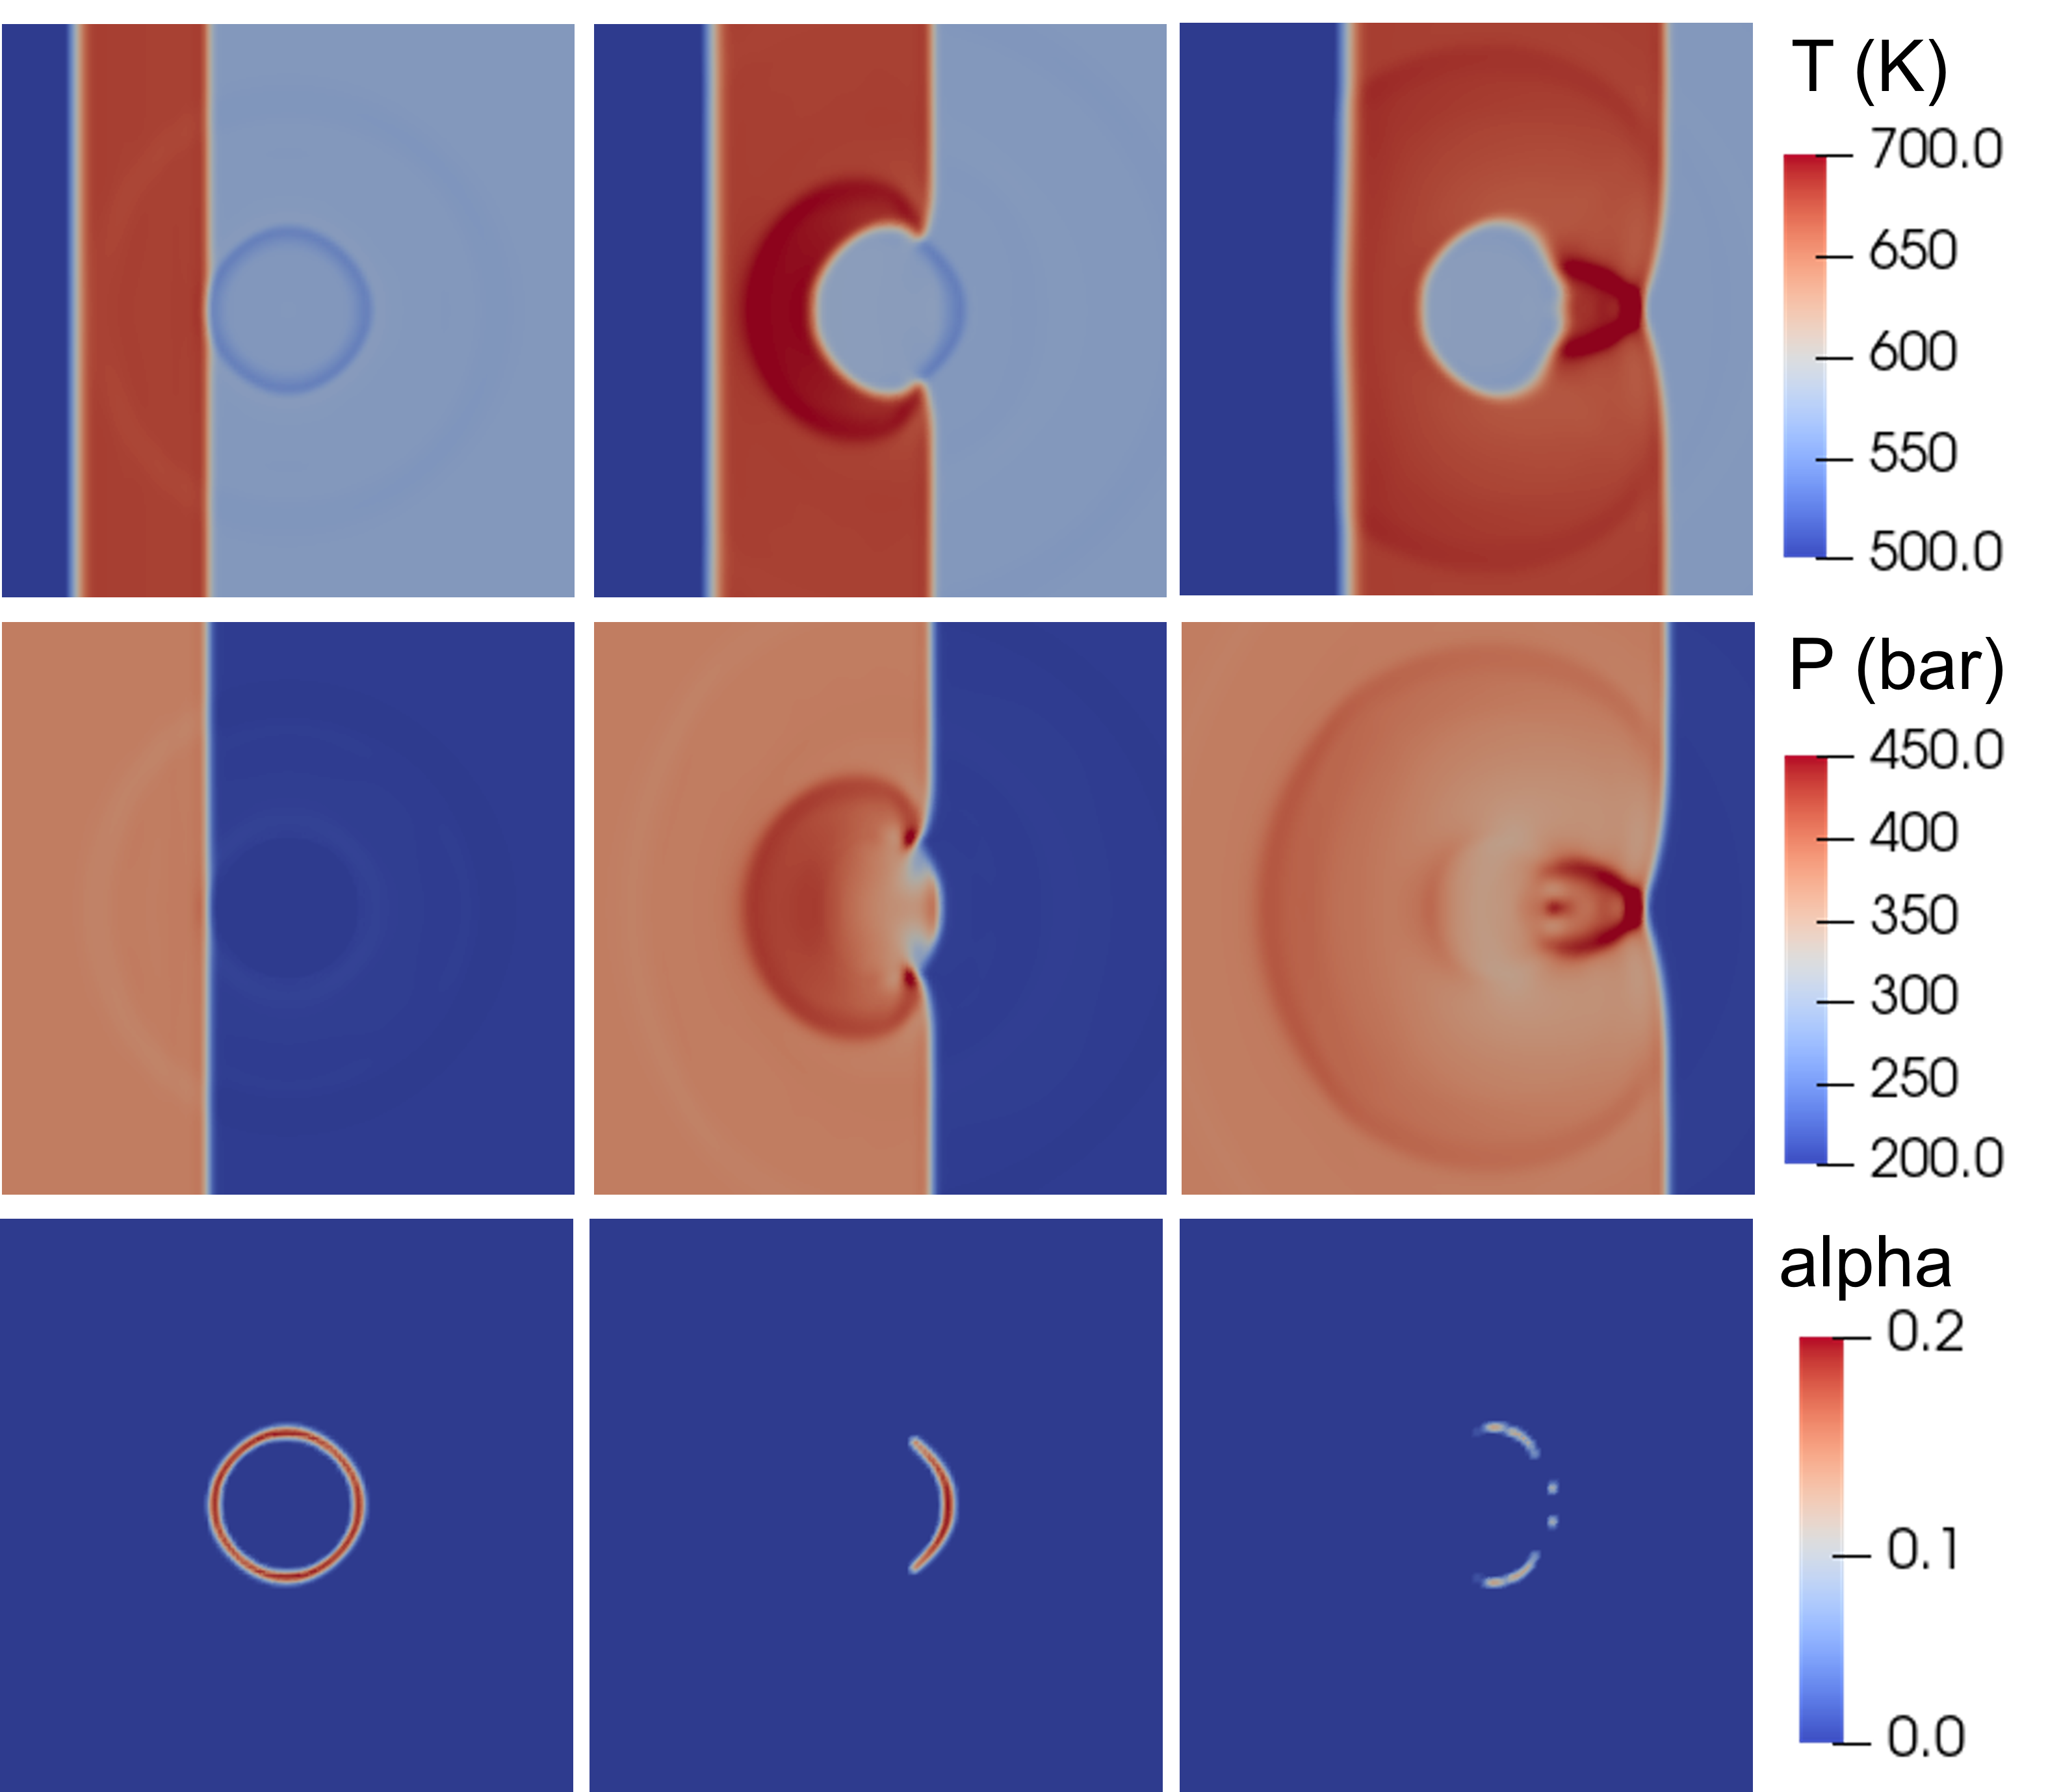
\includegraphics[width=0.65\linewidth]{3D_shock_2C_2.png}
\caption{Transcritical shock-droplet interaction simulation with an initial temperature is 565K, and the droplet consists of 60\%\ce{n-C12H26} and 40\%\ce{n-C8H18} (by mole): the top figures are density, and the bottom figures are $\alpha$, where $\alpha = \beta (1-\beta)$ is a two-phase interface indicator. From left to right are the time instants of $5\times 10^{-7}$ s, $8.3\times 10^{-7}$ s, $120\times 10^{-7}$ s.}
\label{droplet_3d_2C} 
\end{figure}

\begin{figure}[htbp]
\centering
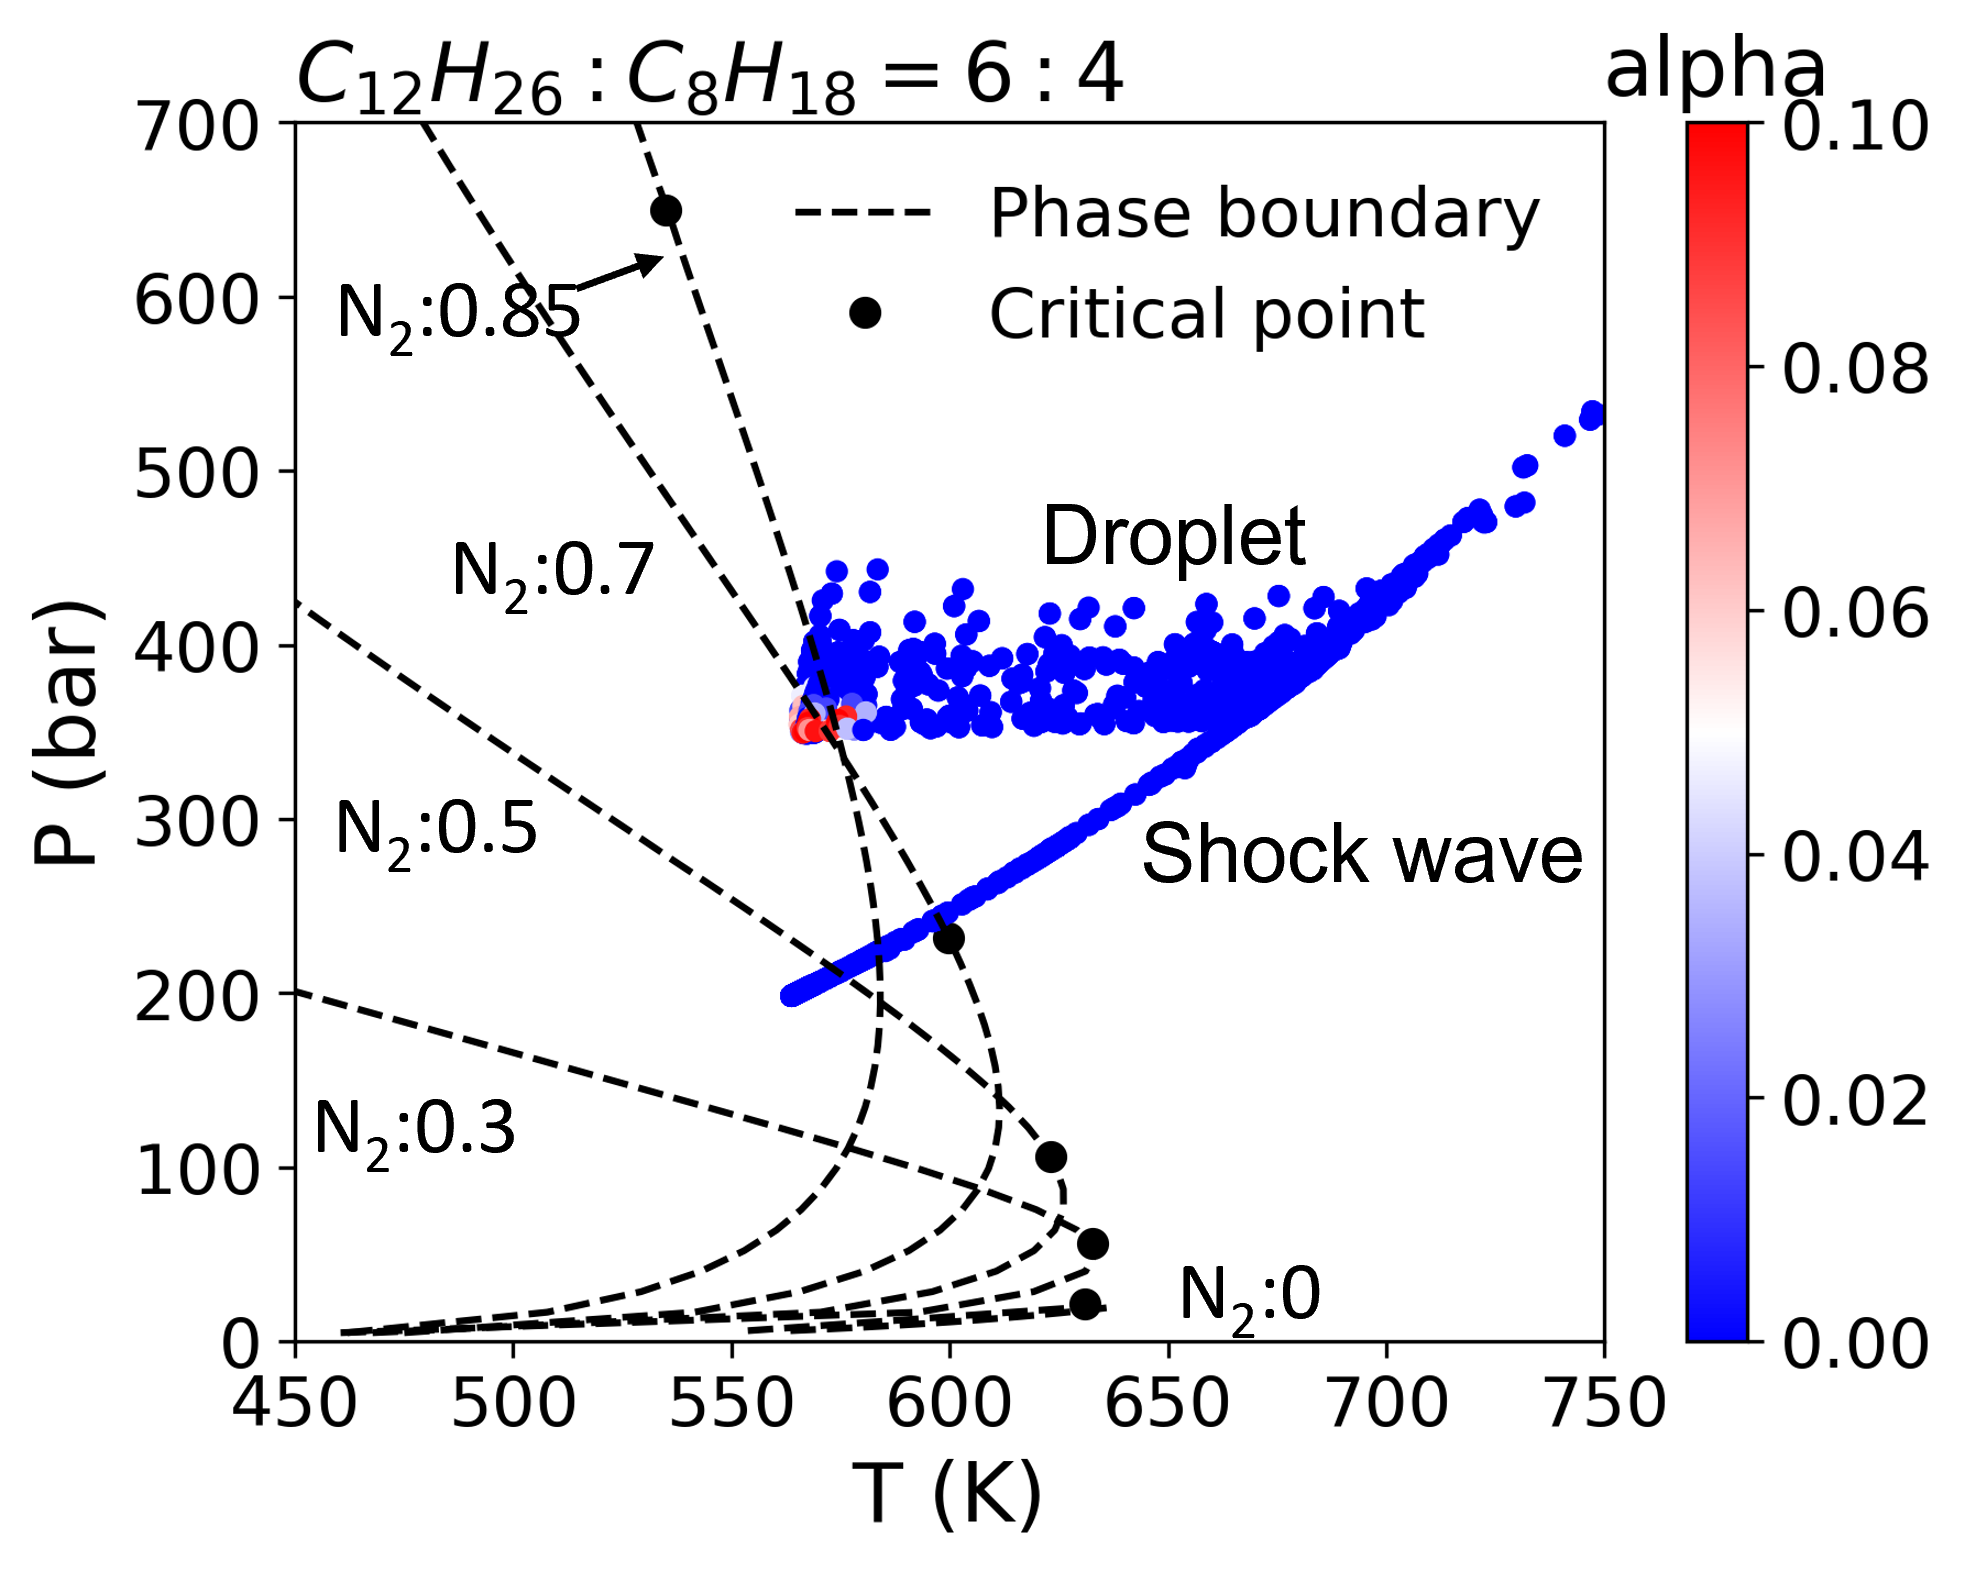
\includegraphics[width=0.50\linewidth]{TP_2C_2_p.png}
\caption{Phase diagram of transcritical shock-droplet interaction simulation with an initial temperature of 565K, and the droplet consists of 70\%\ce{n-C12H26} and 30\%\ce{n-C8H18} (by mass). Data points are taken from the time instance of $1.2\times 10^{-6}$ s. The labels in the figure are mole fractions.}
\label{droplet_3D_2C_phasediagram} 
\end{figure}

The 3D transcritical shock-droplet interaction simulations with a single-component droplet and an initial temperature of 565 K were conducted using 128 CPU cores. The performance of the ISAT-VLE method is illustrated in Fig.~\ref{droplet_3D_perf}. Initially, the ISAT-VLE case exhibited a speed-up of approximately 33 times compared to the VLE case without ISAT. Even in the later stages, it still maintained a significant speed-up of 15 times. On average, the ISAT-VLE method achieved a speed-up factor of approximately 17, showcasing its effectiveness in accelerating the simulations. Furthermore, it is evident that compared with the TML method (as shown in Fig.~\ref{TML_3D_performace}), the computational workload difference between different regions is not as pronounced, making the results closer to those obtained from 2D simulations.


 





\begin{figure}[htbp]
\centering
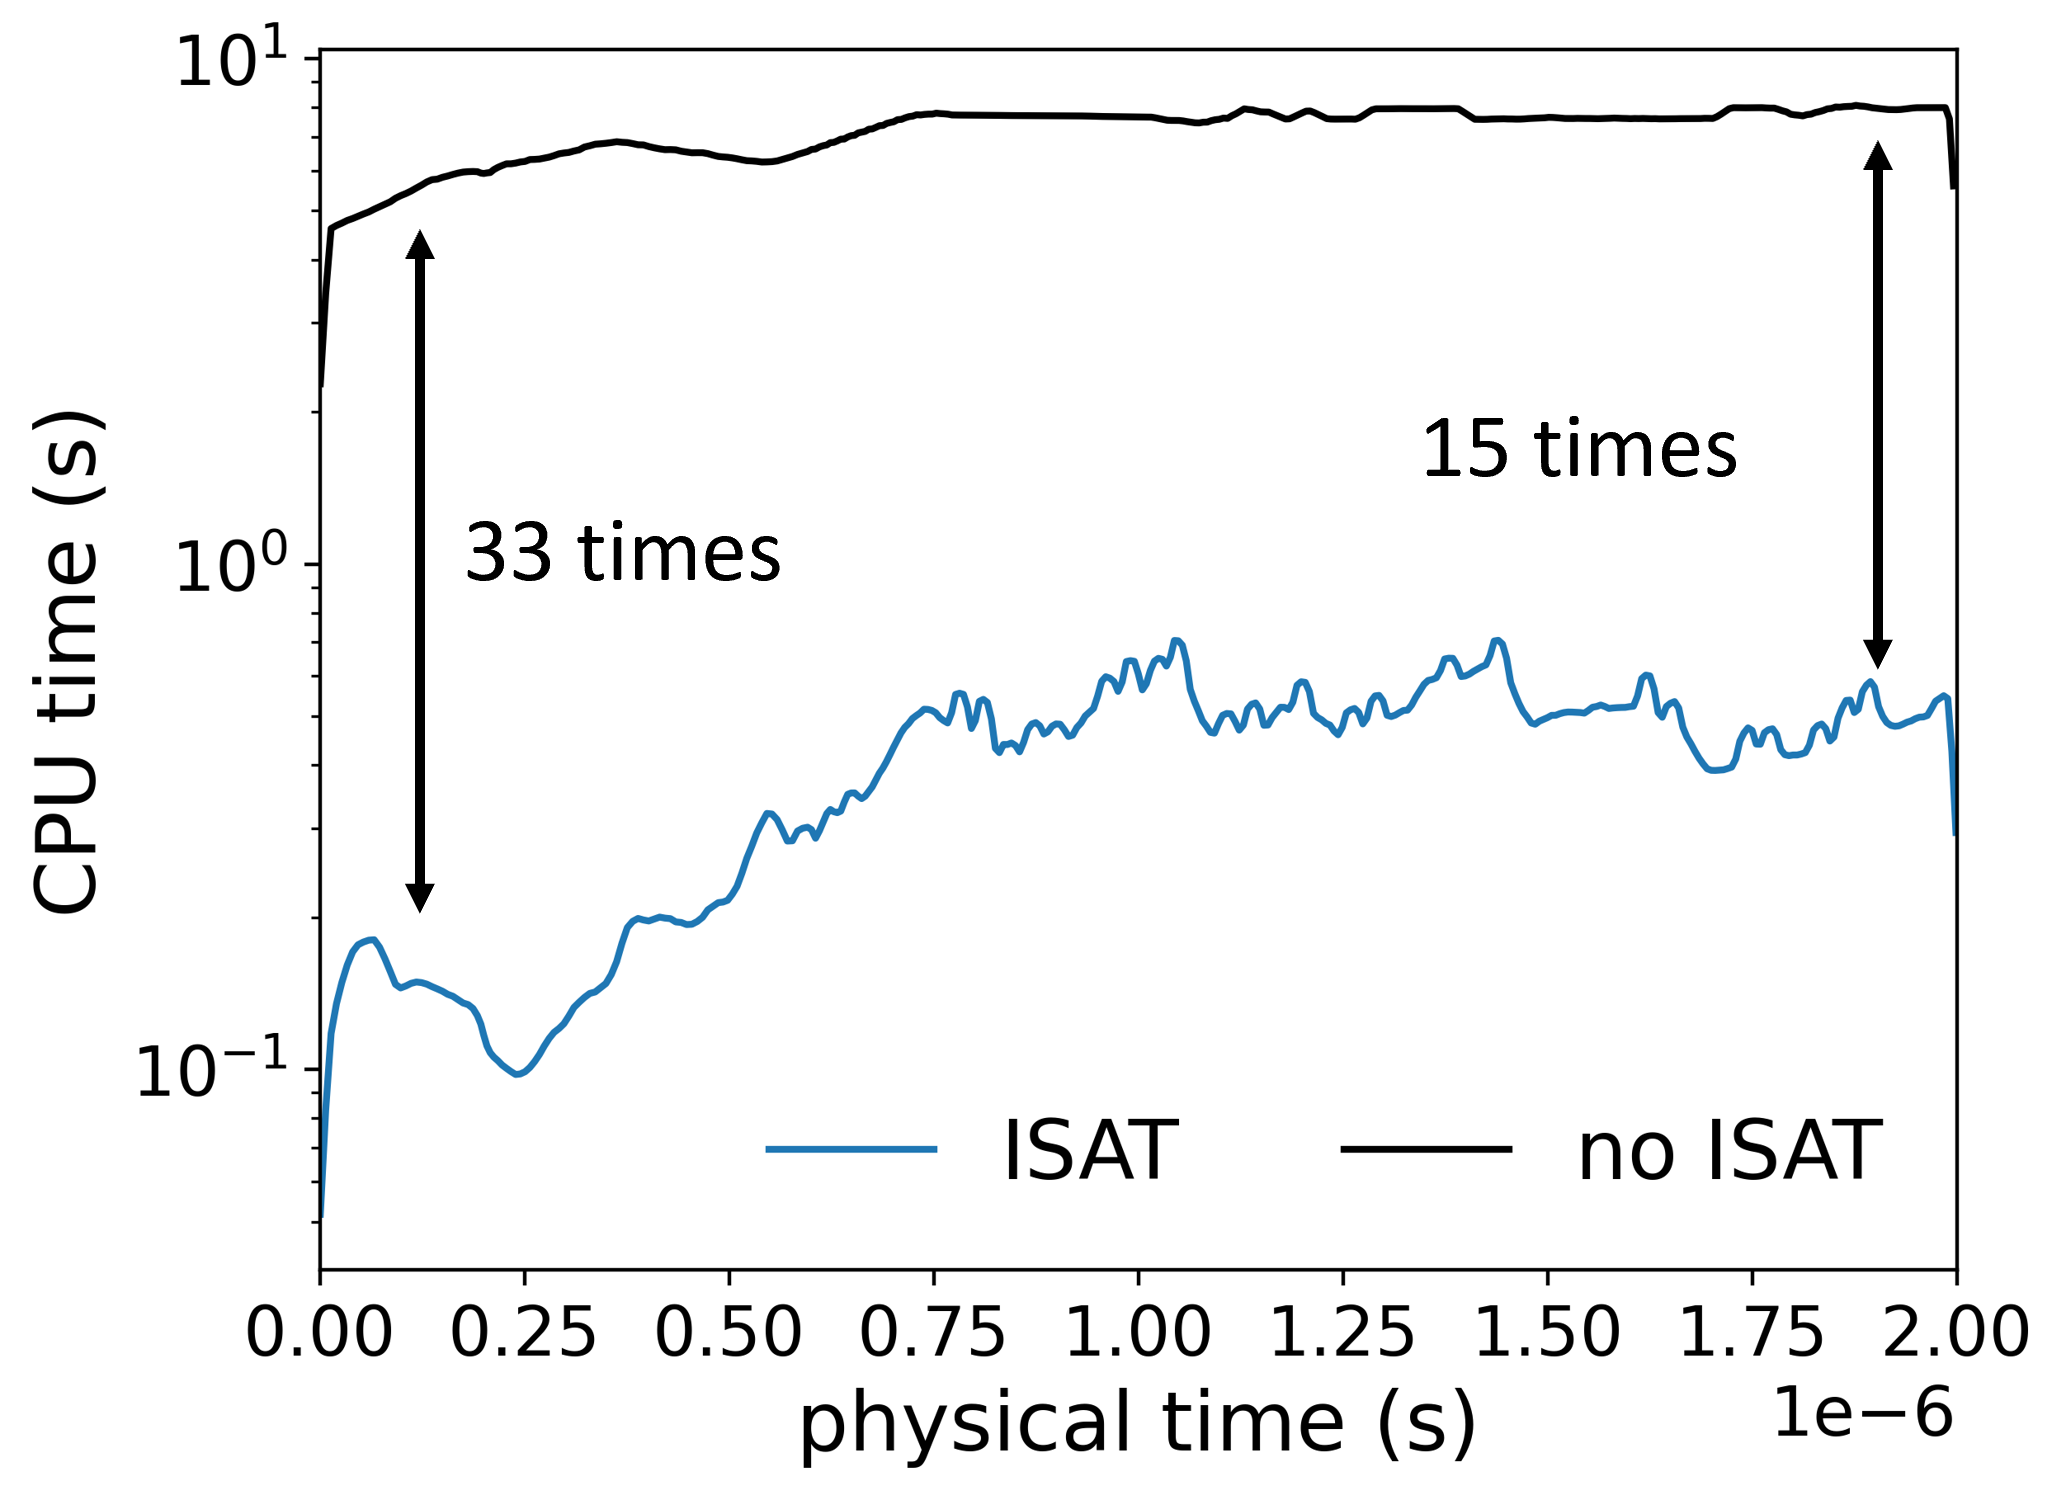
\includegraphics[width=0.5\linewidth]{time_parallel_new.png}
\caption{Performance of the ISAT-VLE method in the 3D transcritical shock-droplet interaction simulation.}
\label{droplet_3D_perf} 
\end{figure}




\section{Conclusions} \label{sec:conclusion}
The vapor-liquid equilibrium (VLE) method is a crucial thermodynamic model for simulating transcritical flows, as it accurately captures phase transitions under high-pressure conditions that are challenging to handle with other methods. However, the computational cost of the VLE method limits its widespread application. Our tests reveal that VLE calculations consume approximately 90\% of the computational resources. In this study, we have developed a new ISAT-VLE model based on the \textit{in situ} adaptive tabulation (ISAT) method to enhance computational efficiency while minimizing memory usage.

We developed ISAT-VLE solvers for both fully conservative (FC) and double flux (DF) schemes. To evaluate the performance and error control of the ISAT-VLE model, we conducted simulations for two significant flow scenarios: transcritical temporal mixing layer (TML) and transcritical shock-droplet interaction. These scenarios represent shearing layers in jet flows and detonation waves, respectively. Both 2D and 3D configurations were employed for testing the ISAT method. 

In TML simulations, the ISAT method accelerated VLE model calculations by a factor of approximately 10, while keeping the maximum error within 1\%. The 3D results demonstrated that the VLE model effectively captured the formation of vortices at the interface and phase separation. In shock-droplet interaction simulations, the ISAT method achieved a larger speedup factor (around 20) and similar error control. 

We also compared the DF method with the FC method. The DF method achieved an even larger speedup factor (about 60). However, the DF method, being a non-conservative scheme, introduced energy errors, leading to greater temperature oscillations at the contact discontinuities. When choosing a method, if the results are temperature-sensitive, the FC scheme should be considered; otherwise, the DF scheme is a good choice. In some cases, the strong spurious pressure oscillation caused the simulations to crash, and the DF scheme proved effective in addressing this issue. However, it is important to note that neither fully conservative schemes nor quasi-conservative schemes (represented by the DF scheme) can perfectly solve the problem of spurious pressure oscillations, and the development of new methods is still required.

New record deletion methods have been proposed to enhance the search performance by accurately detecting and quickly removing redundant records. These methods involve active deletion of records that have not been accessed within a specified number of recent time steps, along with adaptive updates to the maximum table size. To facilitate the implementation of these methods, a data structure has been devised using a combination of a circular array and linked lists, enabling efficient support for various operations. These novel methods result in a performance improvement of 6\% over the already highly optimized ISAT algorithm.

We further investigated the results under different initial temperature conditions in shock-droplet interaction simulations. The findings showed that under appropriate conditions, the high temperature and pressure generated by the shock wave could push a droplet of \ce{n-C12H26} into the supercritical state, eliminating the two-phase interface. In this state, droplet breakup is primarily governed by diffusion. Additionally, we changed the configuration by replacing the \ce{n-C12H26} droplet with an \ce{n-C12H26}/\ce{n-C8H18} mixture droplet. Due to the change in components, this mixture droplet entered the supercritical state at a lower temperature.

Moreover, we observed an intriguing phenomenon. After the shock wave passed through the droplet, a low-temperature and low-pressure annular section persisted at the back of the droplet for a certain period. Under specific conditions, the absence of phase separation occurred at the droplet interface except for the annular region, while the annular region still exhibited a two-phase boundary. This implies that droplet breakup in such cases may be influenced by both the interface effect and the diffusion effect.

In conclusion, the ISAT-VLE model developed in this study achieves significant acceleration in simulations while maintaining error control within 1\% or lower, enabling more complex transcritical VLE simulations.


\section{Analytical framework for VLE} 
\label{App:VLE}
The analytical framework is based on the following derivatives:
\begin{align}
\left(\frac{\partial x_k}{\partial T}\right)_{P,\mathbf{z}},\left(\frac{\partial y_k}{\partial T}\right)_{P,\mathbf{z}},\left(\frac{\partial x_k}{\partial P}\right)_{T,\mathbf{z}},\left(\frac{\partial y_k}{\partial P}\right)_{T,\mathbf{z}},\left(\frac{\partial x_k}{\partial z_i}\right)_{T,P,z_{s,s\neq i}},\left(\frac{\partial y_k}{\partial z_i}\right)_{T,P,z_{s,s\neq i}} \label{eq:app:6derivatives}
\end{align}
To obtain them, we follow Tudisco and Menon's work \cite{tudisco2020analytical} by calculating the following derivatives. 
\begin{align}
x_{T,k}=\left(\frac{\partial v_k}{\partial T}\right)_{P,\mathbf{z}},\quad
x_{P,k}=\left(\frac{\partial v_k}{\partial P}\right)_{T,\mathbf{z}},\quad
x_{N,j}^i=\left(\frac{\partial N_{j,v}}{\partial N_i}\right)_{T,P,N_{k,k\neq i}}
\end{align}
where $v_k$ is the mole fraction of component $k$ in the vapor phase of the total mixture ($v_k = \beta y_k$), $\mathbf{z}$ is the mixture mole fraction in vector form, 
$N_i$ is the total number of moles of component $i$ in the mixture, and $N_{k,v}$ are the number of moles of component $k$ in vapor phase.

These derivatives are given by the solution of three linear equations:
\begin{align}
\mathbfit{A} \mathbfit{x}_T = \mathbfit{b}_T, \quad
\mathbfit{A} \mathbfit{x}_P = \mathbfit{b}_P, \quad
\mathbfit{C}\mathbfit{x}_N^i=\mathbfit{b}_N^i, i = 1,...,N
\end{align}
where $N$ is the number of species.

The coefficients of linear systems derivatives are shown:
\begin{align}
\mathit{A}_{ik} = \left( 1- \frac{\delta_{ki}z_k}{y_k x_k}\right) +\sum_{j=1}^N\left[(1-\beta)\left(\frac{\partial \ln\phi_{i,v}}{\partial y_j}\right)_{T,P,y_{s,s\neq j}}\left(y_i-\delta_{kj}\right)+\beta\left(\frac{\partial \ln\phi_{i,l}}{\partial x_j}\right)_{T,P,x_{s,s\neq j}}\left(x_j-\delta_{jk}\right)\right]
\end{align}
\begin{align}
C_{kj}=\sum_{s=1}^N\left[\left(\frac{\partial \ln\phi_{k,l}}{\partial x_s}\right)_{T,p,x_{r,r\neq s}}\left(\frac{\delta_{sj}-x_s}{1-\beta}\right)+\left(\frac{\partial \ln\phi_{k,v}}{\partial y_s}\right)_{T,p,y_{r,r\neq s}}\left(\frac{\delta_{sj}-y_s}{\beta}\right)\right] +\frac{1}{x_k}\frac{\delta_{kj}-x_k}{1-\beta}+\frac{1}{y_k}\frac{\delta_{kj}-y_k}{\beta}
\end{align}
\begin{align}
b_{T,i}=\beta(1-\beta)\left[\left(\frac{\partial \ln\phi_{i,v}}{\partial T}\right)_{P,\mathbf{y}}-\left(\frac{\partial \ln\phi_{i,l}}{\partial T}\right)_{P,\mathbf{x}}\right]&, b_{P,i}=\beta(1-\beta)\left[\left(\frac{\partial \ln\phi_{i,v}}{\partial P}\right)_{T,\mathbf{y}}-\left(\frac{\partial \ln\phi_{i,l}}{\partial P}\right)_{T,\mathbf{x}}\right]
\end{align}

%\begin{align}
%b_{P,i}=\beta(1-\beta)\left[\left(\frac{\partial \ln\phi_{i,v}}{\partial P}\right)_{T,\mathbf{y}}-\left(\frac{\partial \ln\phi_{i,l}}{\partial P}\right)_{T,\mathbf{x}}\right]
%\end{align}

\begin{align}
b_{N,k}^i=\sum_{j=1}^N\delta_{ji}\Bigg\{\sum_{s=1}^N\left[\left(\frac{\partial \ln\phi_{k,l}}{\partial x_s}\right)_{T,p,x_s}\left(\frac{\delta_{sj}-x_s}{1-\beta}\right)\right]+\frac{\delta_{ji}}{x_k}\frac{\delta_{kj}-x_k}{1-\beta}\Bigg\}
\end{align}

These three linear equations are obtained by taking the derivative of the fugacity equation, and the derivatives with respect to pressure and temperature have the same coefficient matrix $A$. The linear systems are solved using the LU decomposition method in the current work.
Using the relation $ \beta = \sum_i v_i$, the $\beta $ derivative is obtained:
\begin{align}
\left(\frac{\partial \beta }{\partial T}\right)_{P,\mathbf{z}} = \sum_{k=1}^N \left(\frac{\partial v_k}{\partial T}\right)_{P,\mathbf{z}},\left(\frac{\partial \beta}{\partial P}\right)_{T,\mathbf{z}} = \sum_{k=1}^N \left(\frac{\partial v_k}{\partial P}\right)_{T,\mathbf{z}} \label{eq:dbetafPT}
\end{align}
And using the relation between $v_i,\beta,x_i,y_i$, first 4 terms in Eq.~\ref{eq:app:6derivatives} can be obtained 
$$\left(\frac{\partial x_i}{\partial T}\right)_{P,\mathbf{z}} = \left(\frac{\partial (z_i-v_i)/(1-\beta)}{\partial T}\right)_{P,\mathbf{z}}= \frac{x_i}{1-\beta}\sum_{k=1}^N\left(1-\frac{\delta_{ik}}{x_k}\right)\left(\frac{\partial v_k}{\partial T}\right)_{P,\mathbf{z}}$$
$$\left(\frac{\partial y_i}{\partial T}\right)_{P,\mathbf{z}} = \left(\frac{\partial v_i/\beta}{\partial T}\right)_{P,\mathbf{z}}= -\frac{y_i}{\beta}\sum_{k=1}^N\left(1-\frac{\delta_{ik}}{y_k}\right)\left(\frac{\partial v_k}{\partial T}\right)_{P,\mathbf{z}}$$
For derivatives with respect to pressure, similar formulas can be used, with all the $\left(\frac{\partial (\cdot)}{\partial T}\right)_{P,\mathbf{z}}$ replaced by $\left(\frac{\partial (\cdot)}{\partial P}\right)_{T,\mathbf{z}}$.

For the last two terms in Eq.~\ref{eq:app:6derivatives}, we need to deal with the constraints of $\mathbf{z}$ ($\sum_i z_i =1$), which makes a single $z_i$ not a free variable. Here we use an extension method to extend $\mathbf{z}$ to the whole positive space:
\begin{equation} 
F(\mathbf{z}) = 
\begin{cases}
 F\left(\mathbf{z}\right)  &\text{if }  \sum_i z_i =1 \\
 F\left(\frac{\mathbf{z}}{\sum_k z_k}\right) & \text{otherwise} 
\end{cases}  
\end{equation}
where $F$ represents any function of mixture mole fraction $z_i$.  With this extension, $F(\mathbf{z}) = F(\mathbf{N})$.  Note that although we extend the function, we only use $\mathbf{z}$ that meets the constraint for calculation, so we can further simplify the results with the constraint $\sum_i z_i =\sum_i N_i = 1$.
%$$\left(\frac{\partial \beta}{\partial z_i}\right)_{T,P,z_{s,s\neq i}}= \frac{\partial\left(\sum_k N_k^v\right)/\left(\sum_k N_k\right)}{\partial N_i}=\frac{1}{\sum_k N_k}\left[\sum_{j=1}^N\left(\frac{\partial N_j^v}{\partial N_i}\right)_{T,P,N_{s,s\neq j}} -\beta\right] =\sum_{j=1}^N\left(\frac{\partial N_j^v}{\partial N_i}\right)_{T,P,N_{s,s\neq j}} -\beta $$
Considering $\beta  = \frac{\sum_k N_{k,v}}{\sum_k N_k}$ gives 
\begin{align}
\left(\frac{\partial \beta}{\partial z_i}\right)_{T,P,z_{s,s\neq i}}=\left(\frac{\partial \frac{\sum_k N_{k,v}}{\sum_k N_{k}}}{\partial N_i}\right)_{T,P,z_{s,s\neq i}}=\sum_{j=1}^N\left(\frac{\partial N_{j,v}}{\partial N_i}\right)_{T,P,N_{s,s\neq j}} -\beta \label{eq:dbetadz}
\end{align}

%$$\left(\frac{\partial y_k}{\partial z_i}\right)_{T,P,z_{s,s\neq i}}= \frac{\partial \frac{N_k^v} { \beta \sum_j N_j}}{\partial N_i} = \frac{1}{\beta \sum_j N_j} \sum_{s=1}^N\left(\delta _{sk}-y_k\right)\left(\frac{\partial N_s^v}{\partial N_i}\right)_{T,P,N_{k,k\neq i}}=\frac{1}{\beta} \sum_{s=1}^N\left(\delta _{sk}-y_k\right)\left(\frac{\partial N_s^v}{\partial N_i}\right)_{T,P,N_{k,k\neq i}}$$
Noticing the relation $y_k=\frac{N_{k,v}} { \beta \sum_j N_j}$ and $x_k=\frac{N_k-N_{k,v}} { (1-\beta) \sum_j N_j}$, the last two term can be derived:
\begin{align}\left(\frac{\partial y_k}{\partial z_i}\right)_{T,P,z_{s,s\neq i}}= \frac{\partial \frac{N_{k,v}} { \beta \sum_j N_j}}{\partial N_i}=\frac{1}{\beta} \sum_{j=1}^N\left(\delta _{jk}-y_k\right)\left(\frac{\partial N_{j,v}}{\partial N_i}\right)_{T,P,N_{s,s\neq j}}
\end{align}

%$$\left(\frac{\partial x_k}{\partial z_i}\right)_{T,P,z_{s,s\neq i}}= \frac{\partial \frac{N_k-N_k^v} { (1-\beta) \sum_j N_j}}{\partial N_i} = \frac{1}{(1-\beta) \sum_j N_j} \left[\sum_{s=1}^N\left(\delta _{sk}-y_k\right)\left(\frac{\partial N_s^v}{\partial N_i}\right)_{T,P,N_{k,k\neq i}}+\delta_{ik}-x_k\right]=\frac{1}{1-\beta} \sum_{s=1}^N\left(x_k-\delta_{sk}\right)\left(\frac{\partial N_s^v}{\partial N_i}\right)_{T,P,N_{k,k\neq i}}$$

\begin{align}\left(\frac{\partial x_k}{\partial z_i}\right)_{T,P,z_{s,s\neq i}}= \frac{\partial \frac{N_k-N_{k,v}} { (1-\beta) \sum_j N_j}}{\partial N_i} = \frac{1}{(1-\beta) } \left[\sum_{s=1}^N\left(x_k - \delta _{jk}\right)\left(\frac{\partial N_{j,v}}{\partial N_i}\right)_{T,P,N_{s,s\neq j}}+\delta_{ik}-x_k\right]
\end{align}

\section{Grid convergence study} 


\subsection{Transcritical temporal mixing layer} 
\label{App:TML}

We performed a grid convergence study for transcritical temporal mixing layer simulations using the configuration of Case 1 in Tab.~\ref{TML_init_table}. Two additional meshes were generated based on the original mesh, with one being refined by a factor of two in each direction and the other coarsened by a factor of two in each direction. To compare the results obtained from these three meshes, we analyzed the momentum thickness defined as:

\begin{align}
\delta_m = \frac{\displaystyle\int_{z_{min}}^{z_{max}}\left[\langle \rho u_x \rangle_{z_{max}} - \langle \rho u_x \rangle\right]\left[\langle \rho u_x \rangle - \langle \rho u_x \rangle_{z_{min}}\right]\mathrm{d}z}{\left(\langle \rho u_x \rangle_{z_{max}} - \langle \rho u_x \rangle_{z_{min}}\right)^2}
\end{align}

which is a measure of mixing layer growth, where $\langle\rangle$ symbolizes averages over $(x,y)$ planes.

The momentum thicknesses of three meshes versus time are presented in Fig.~\ref{TML_GC}, and exhibit a maximum relative error of approximately 4.4\%. The meshes with different resolutions do not have a significant impact on the results.

\begin{figure}[htbp]
\centering
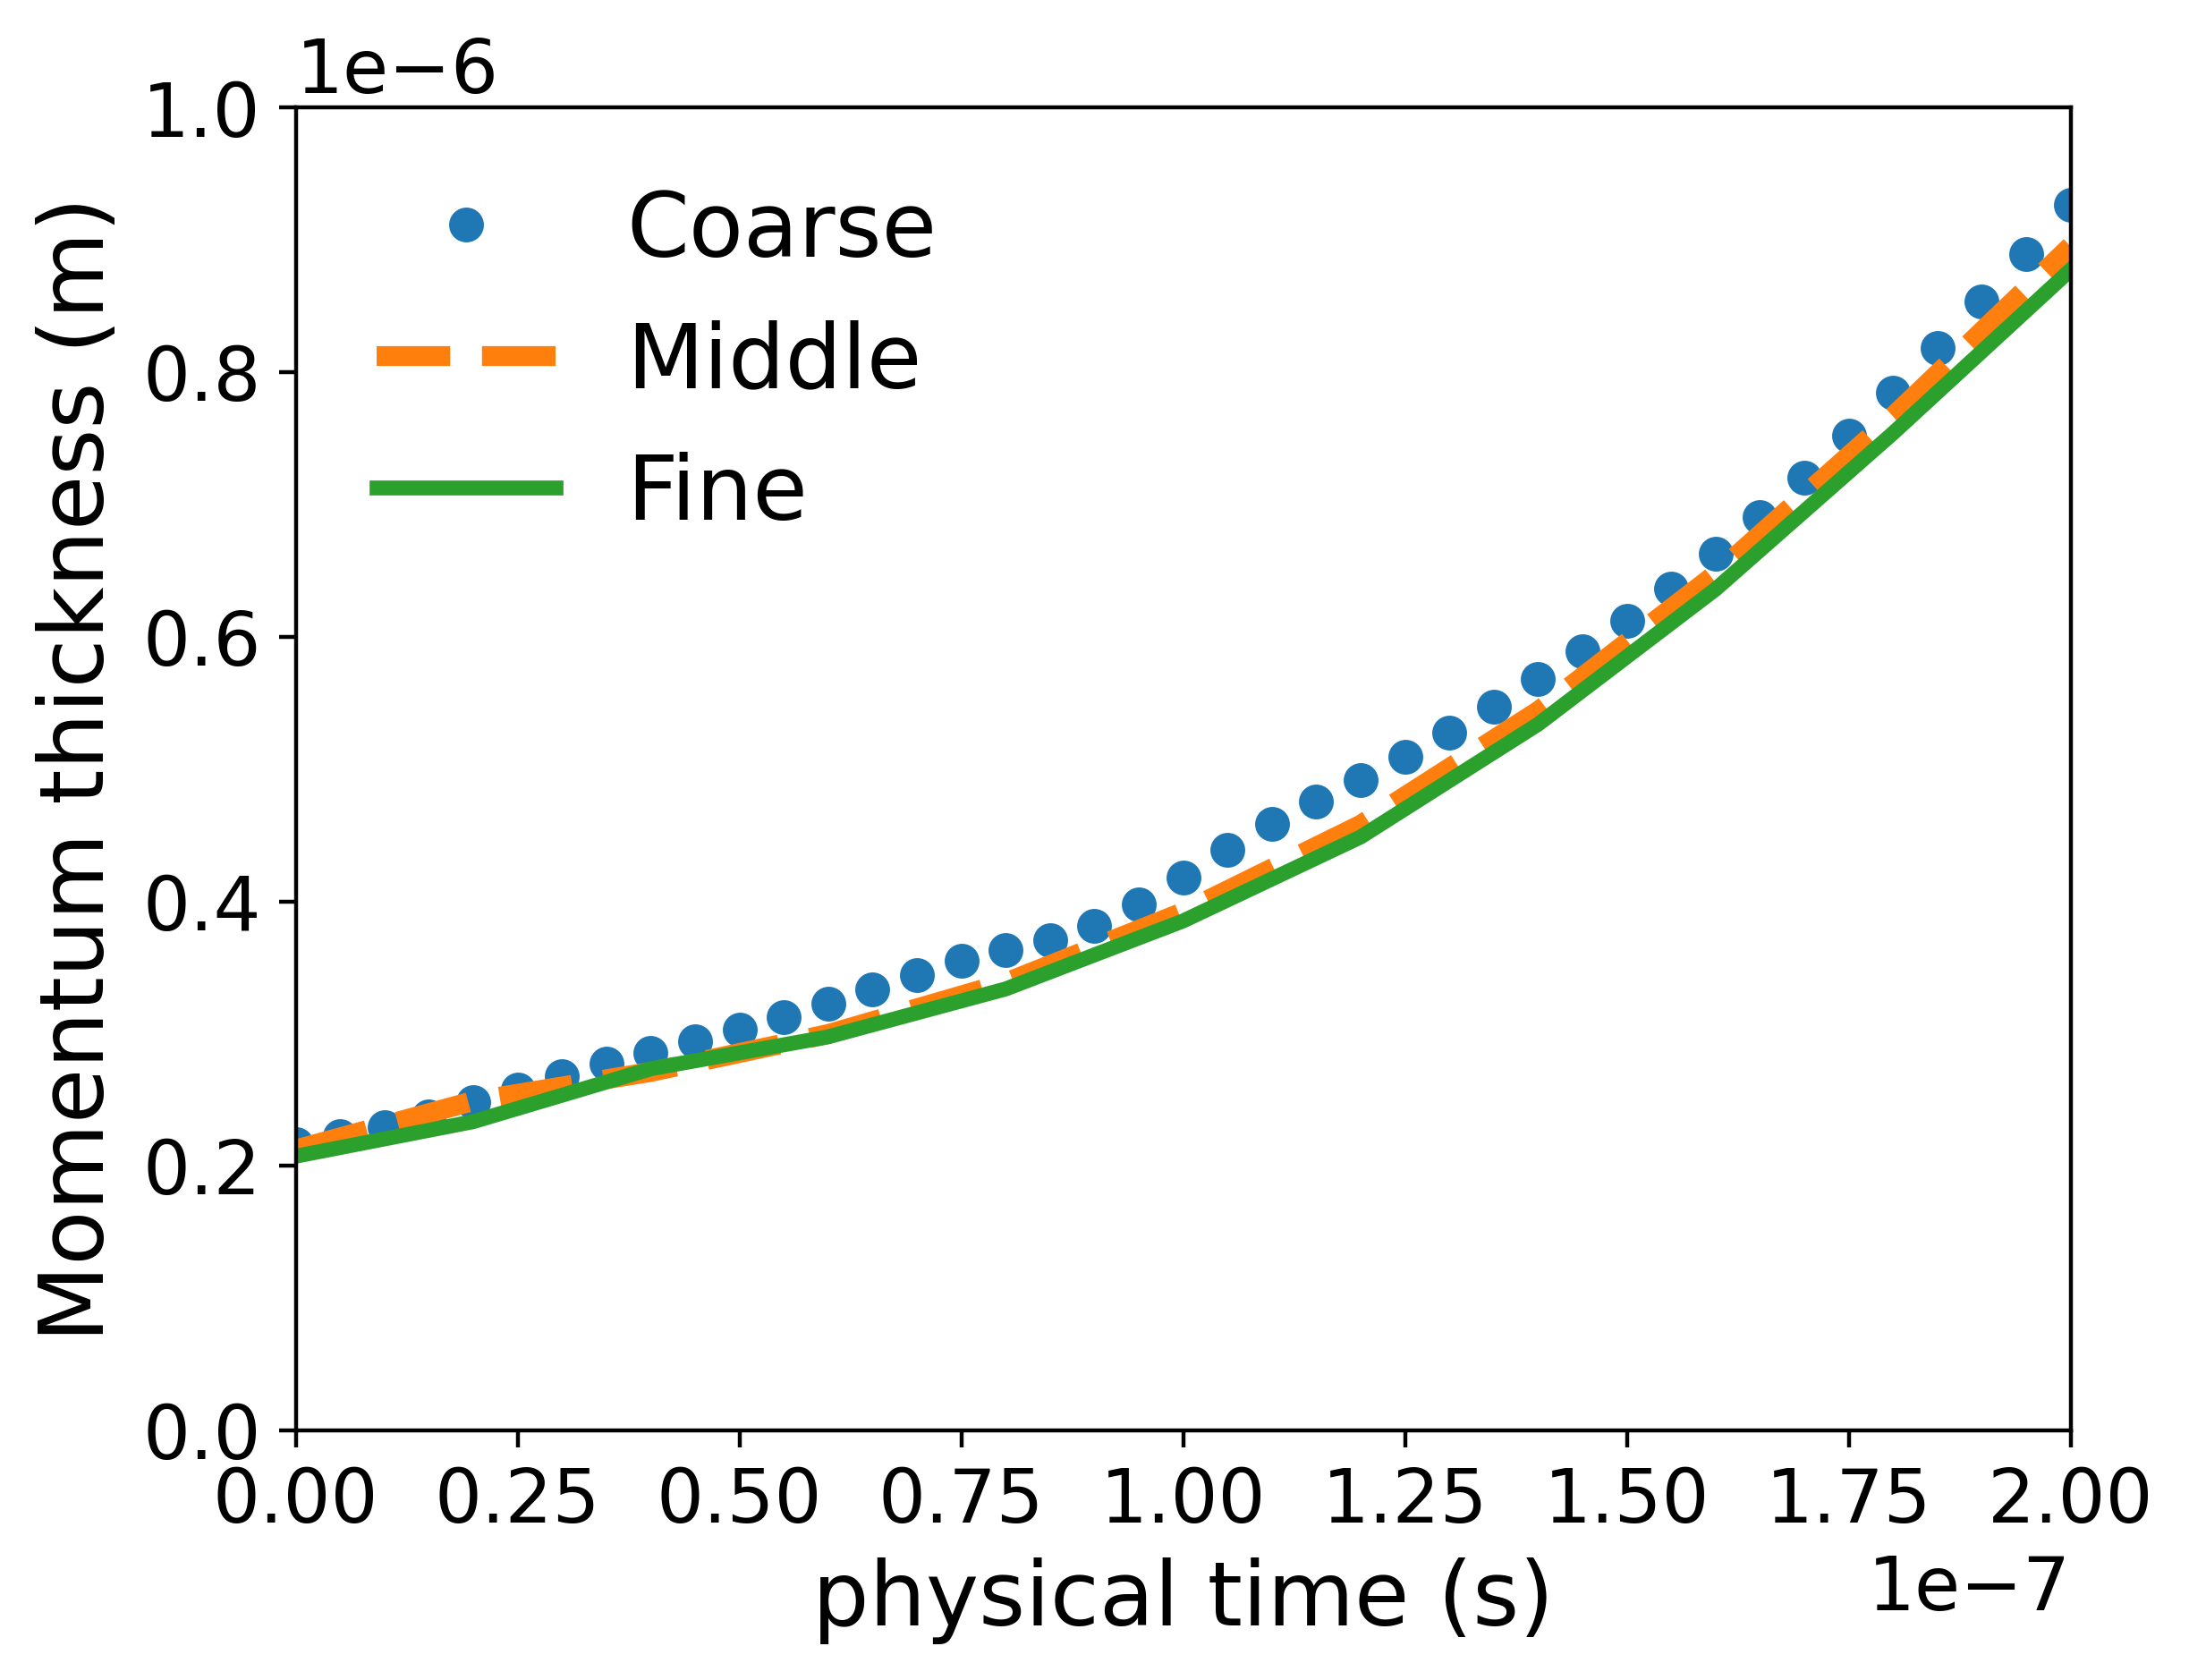
\includegraphics[width=0.4\linewidth]{TML_GC_mt.png}
\caption{Comparison of the TML momentum thickness for 3 meshes.}
\label{TML_GC} 
\end{figure}

\subsection{Transcritical shock-droplet interaction} 
\label{App:SD}


We conducted a grid convergence study using the \ce{n-C12H26} droplet grid setup as described in Sec.~\ref{sec:SD}. The simulations were performed using the fully conservative scheme solver. Based on the base mesh with dimensions of 256 × 256 × 256, we refined and coarsened the mesh by a factor of two in each direction, obtaining two additional meshes. In order to assess the impact of these meshes, we compared the properties along the centerline in the x-direction when the shock wave reached the center of the droplet ($t=6.6\times 10^{-7}$). In Fig.\ref{SG_GC}, The density, temperature, and pressure curves didn't exhibit obvious differences among the different meshes, with a relative error of approximately 5\%.


\begin{figure}[htbp]
\centering
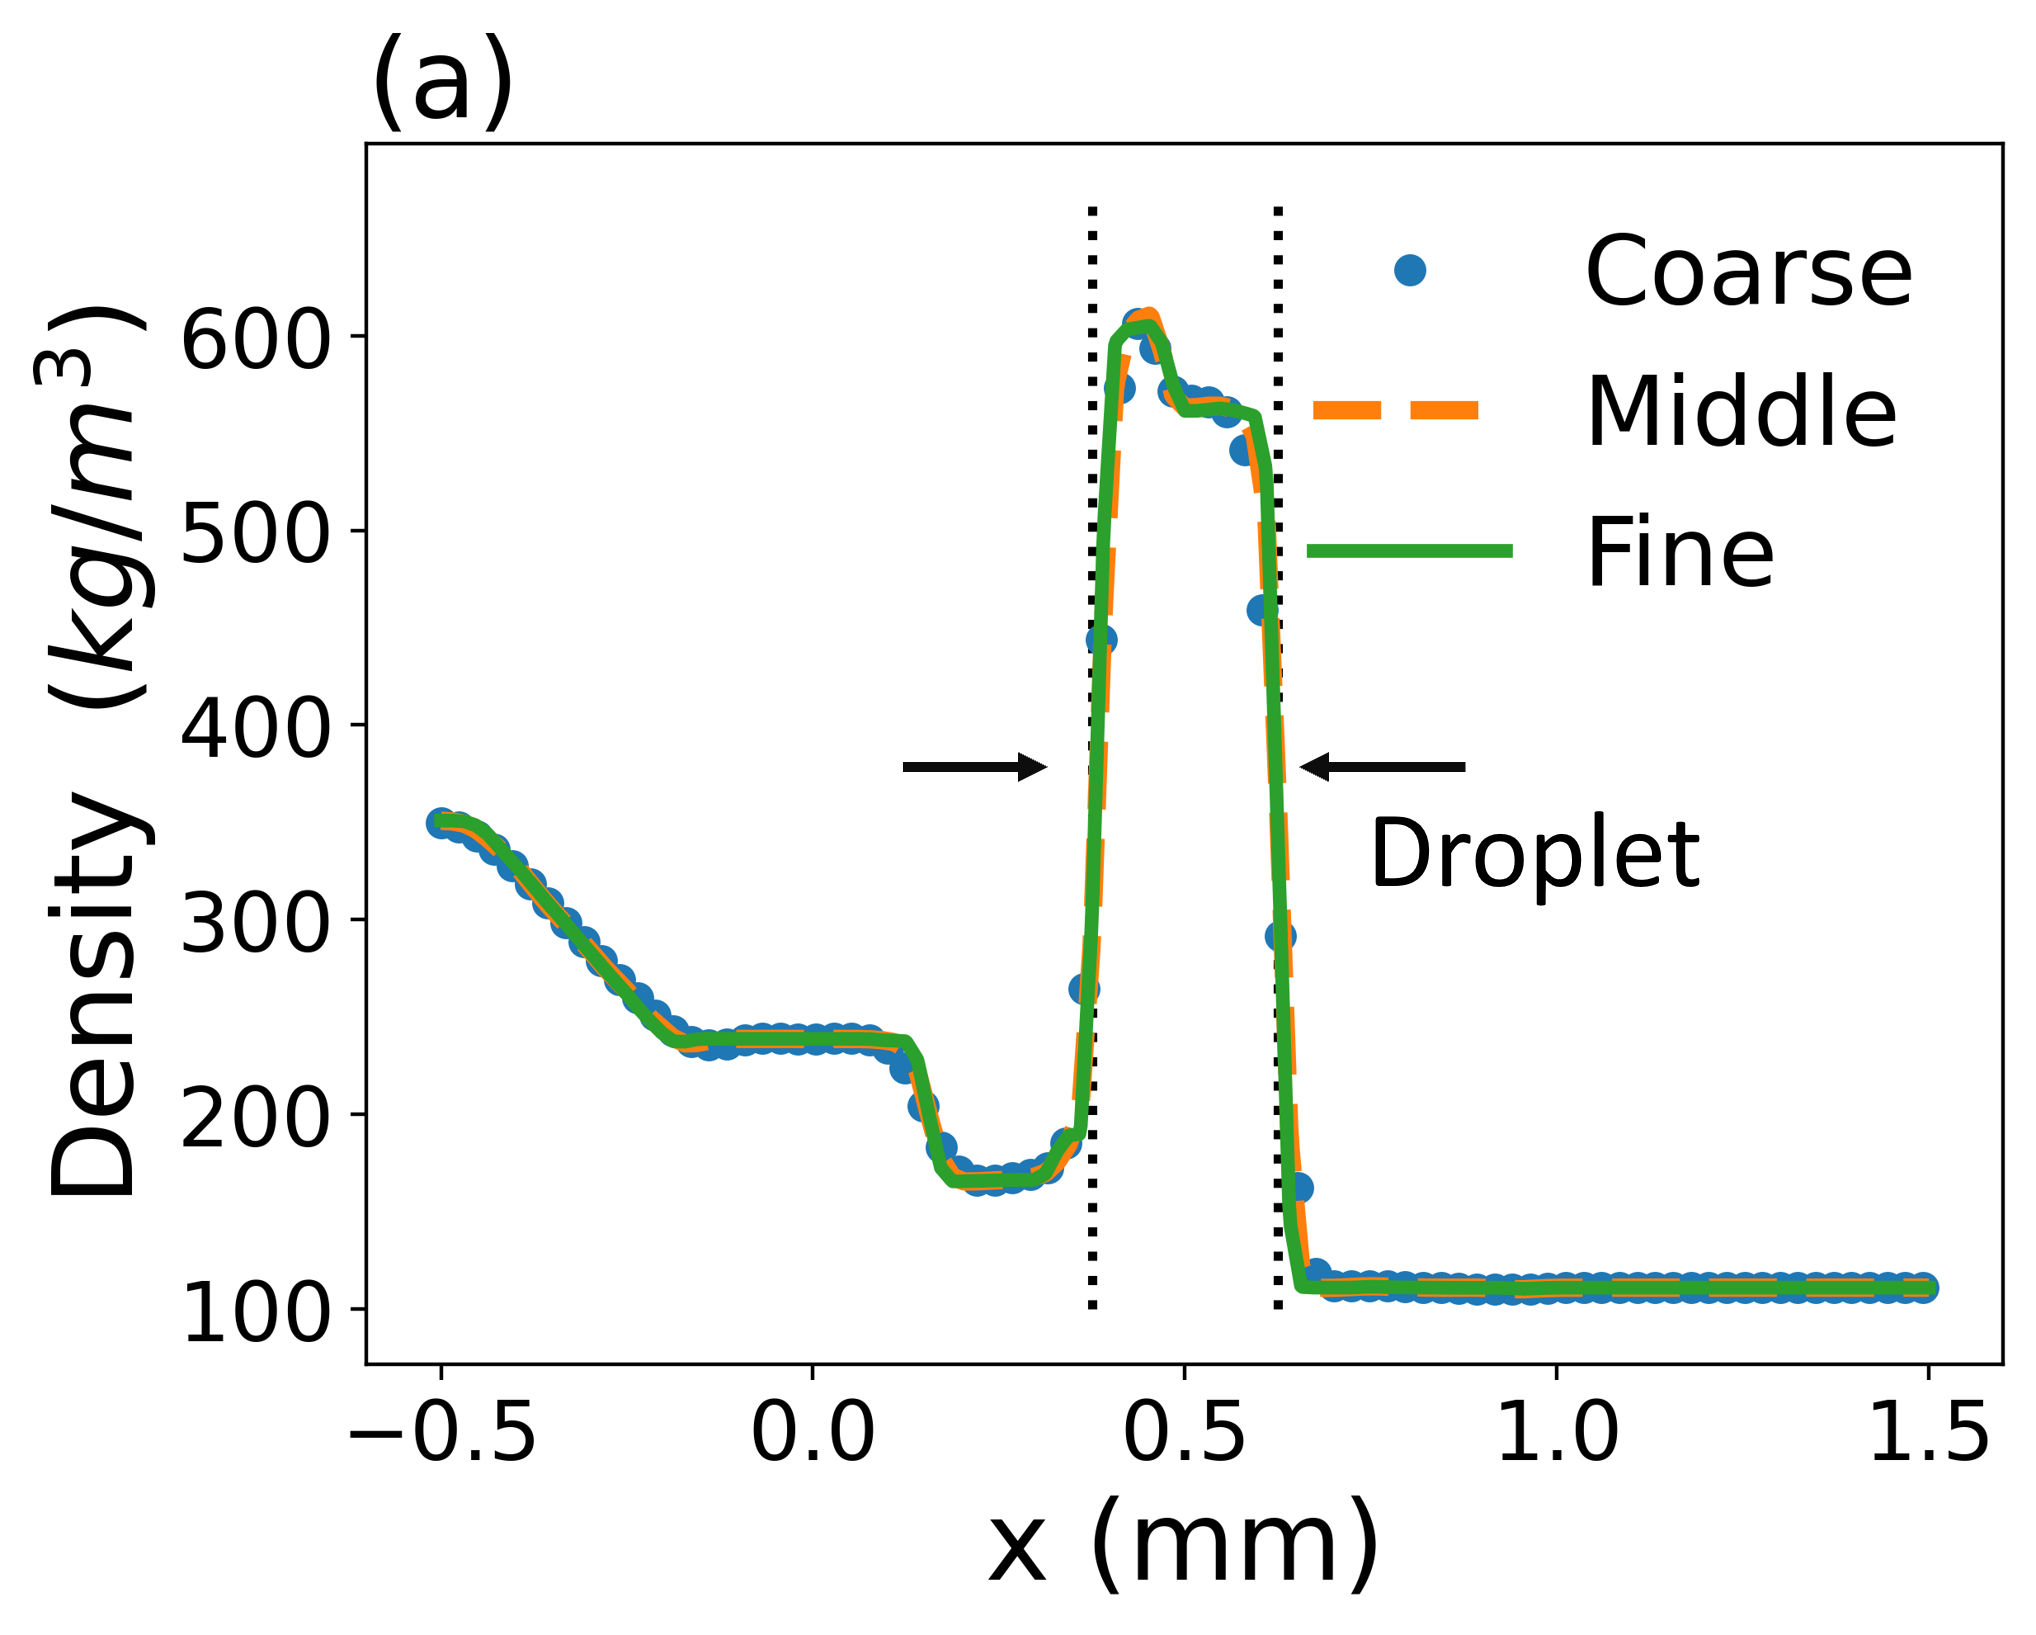
\includegraphics[width=0.3\linewidth]{SD_GC_d_p.png}
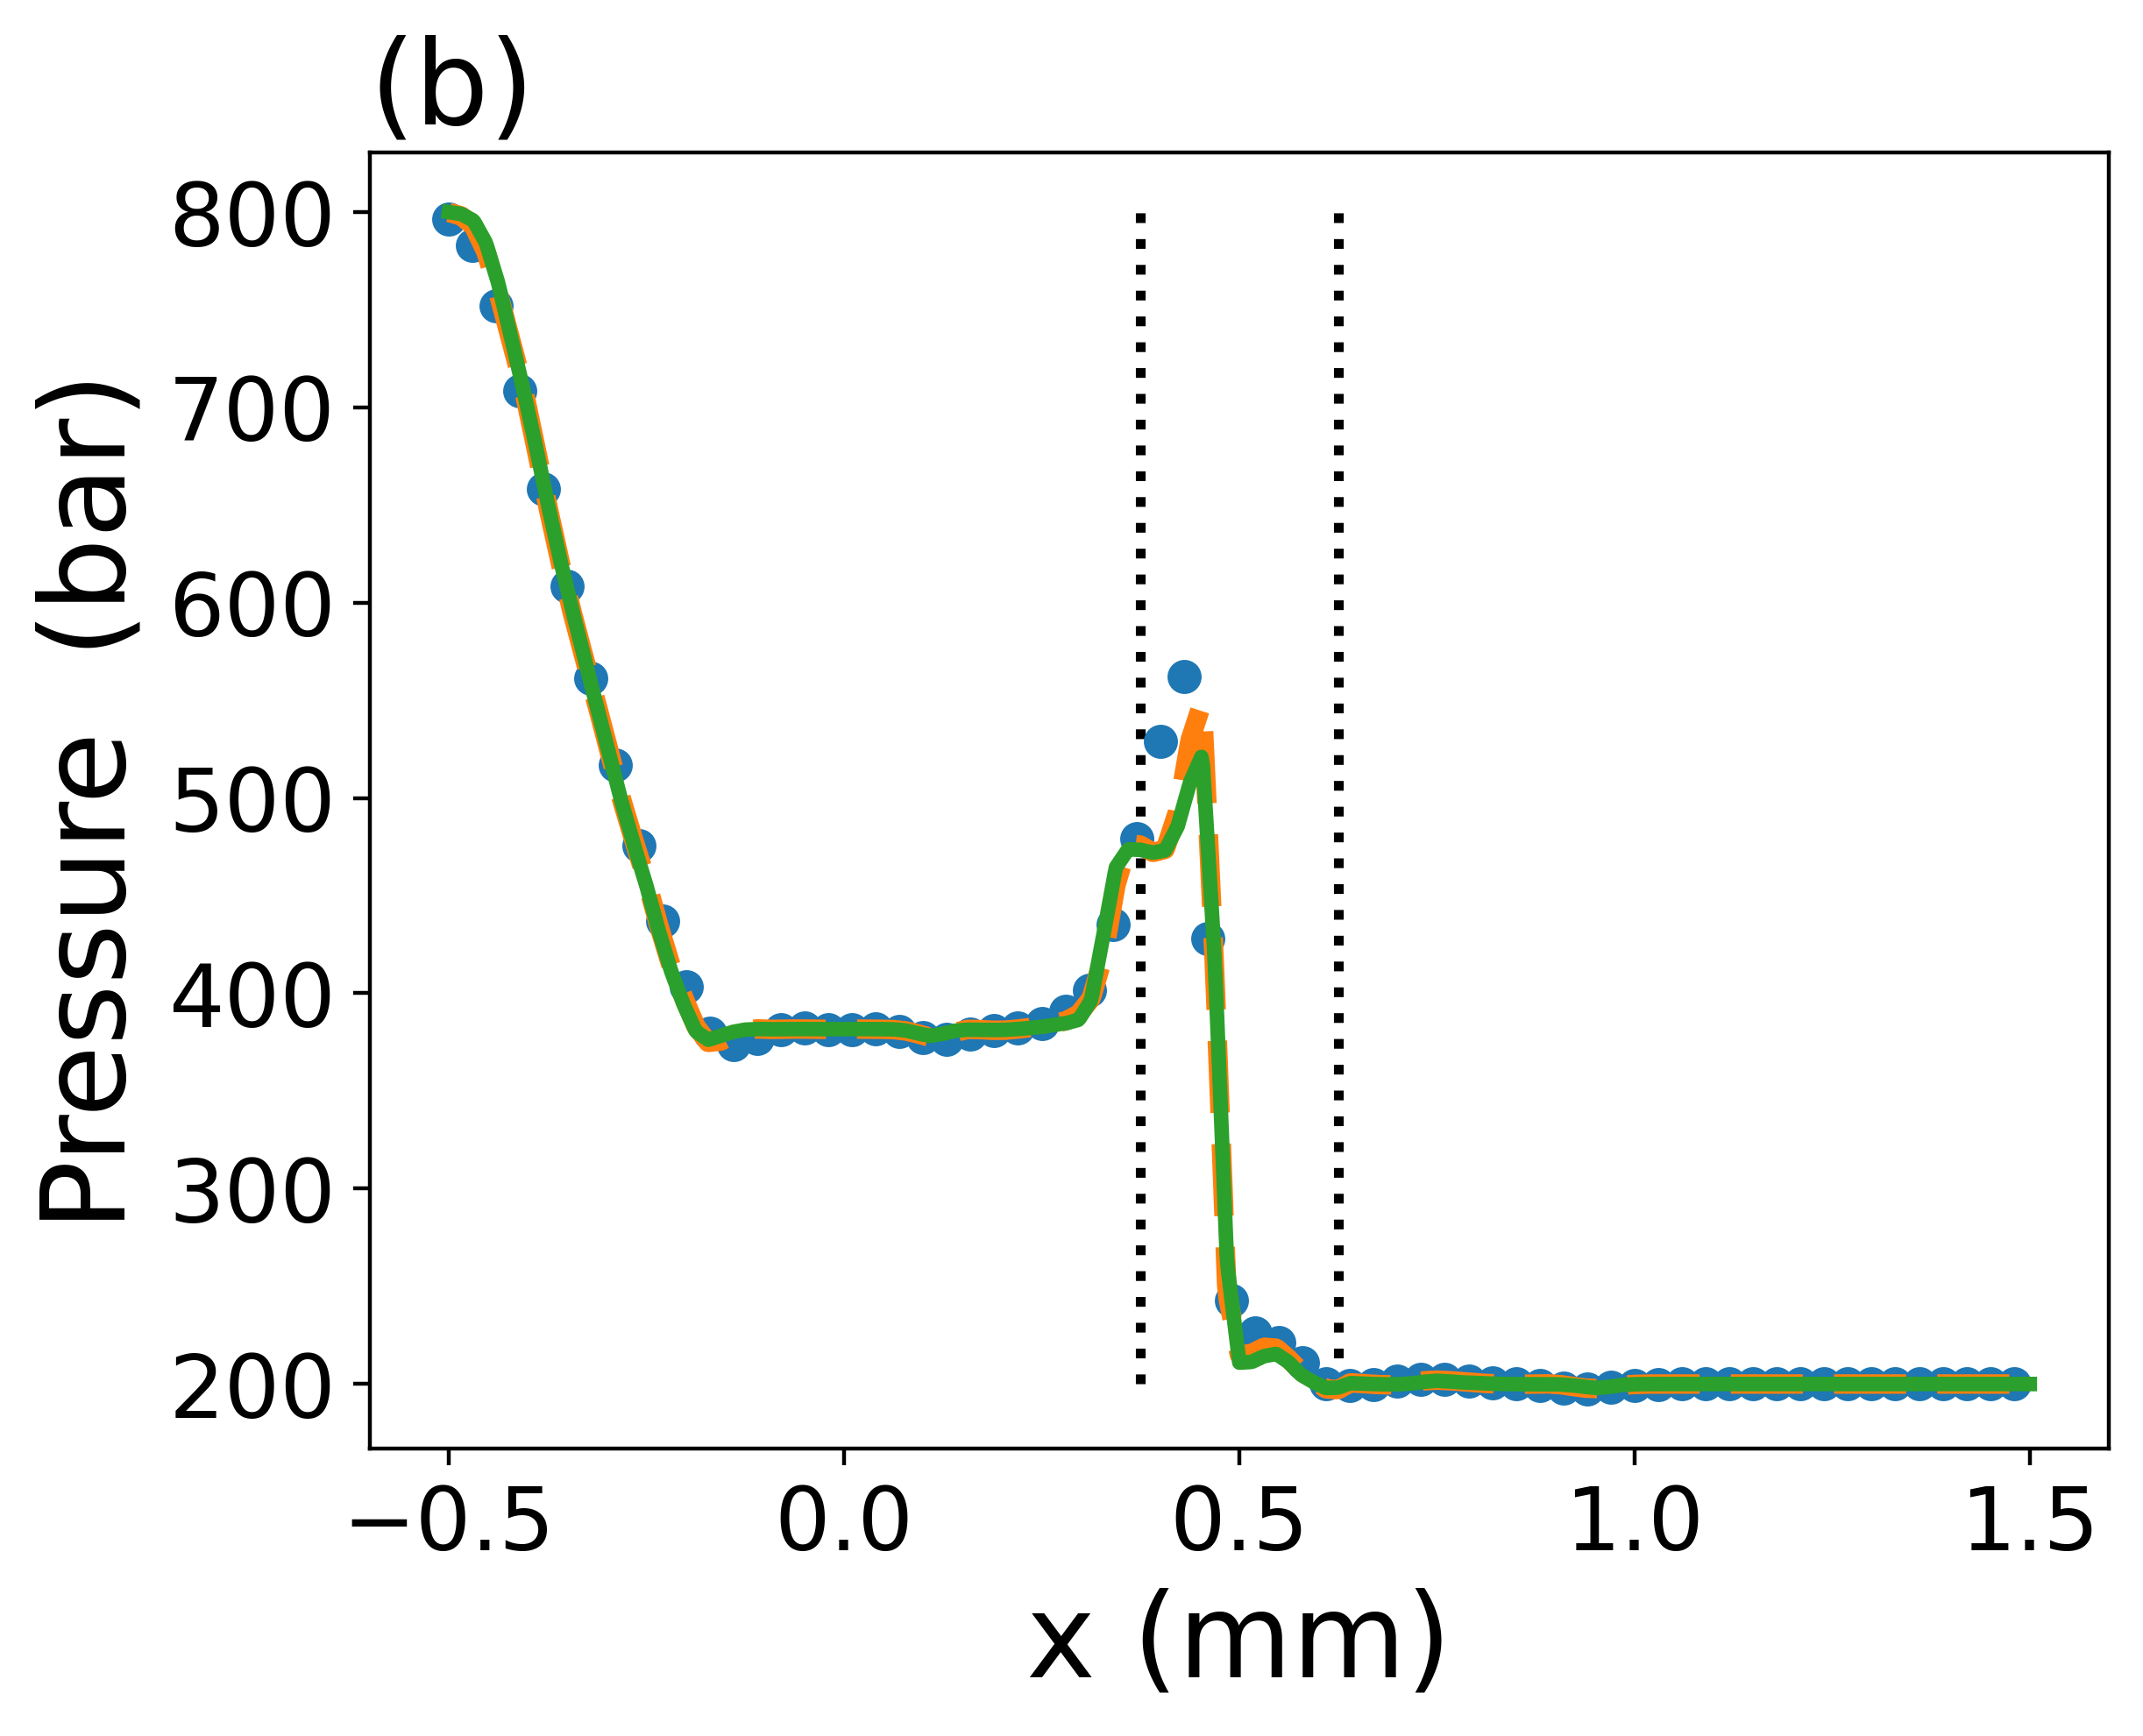
\includegraphics[width=0.3\linewidth]{SD_GC_p.png}
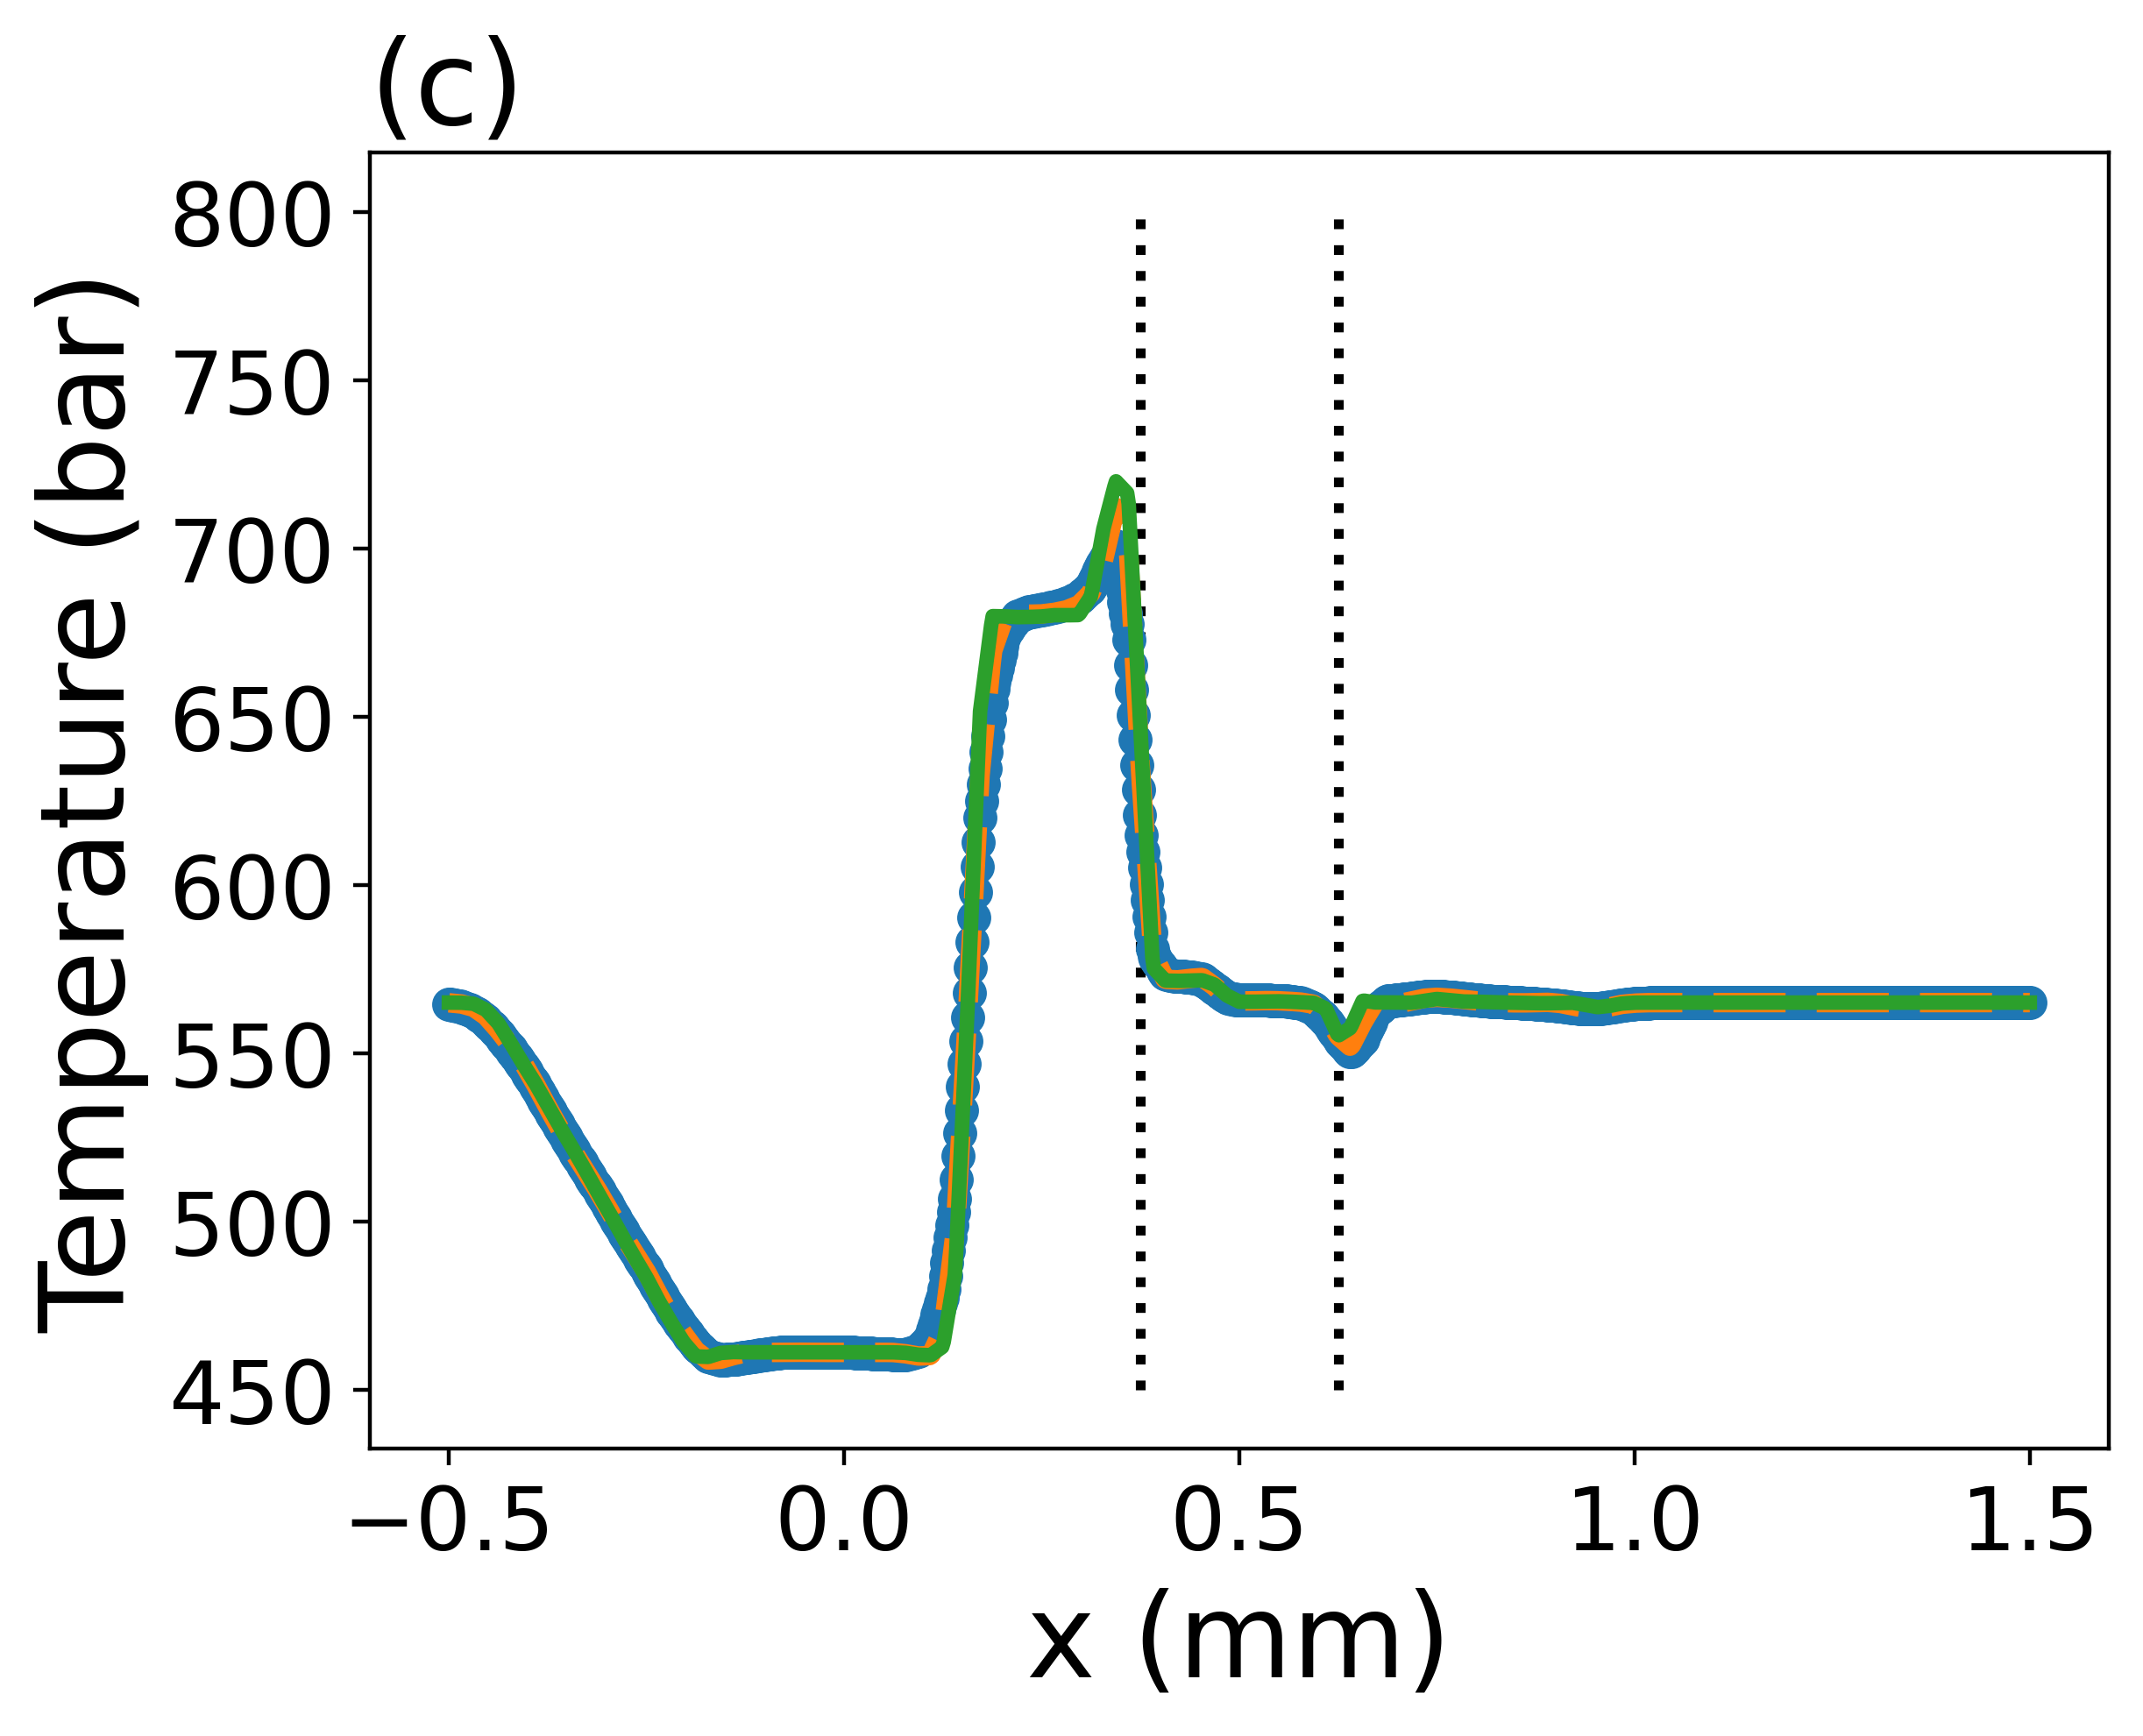
\includegraphics[width=0.3\linewidth]{SD_GC_t.png}
\caption{Comparison of 3D shock-droplet interaction results on the centerline along the x direction for 3 meshes.}
\label{SG_GC} 
\end{figure}

\begin{itemize}

%\item Chapter 1 introduces the analytic goals pursued in this thesis.

\item Chapter 2 briefly presents the history of, and science behind, the
subjects presented in this thesis.

\item In Chapter 3 the experiment is outlined.

\item Chapter 4 describes the simulation process used in the analysis.

\item Chapter 5 follows the chain of reconstruction software used to obtain
meaningful results from data.

\item Chapter 6 hashes out the strategy for analysis and presents the data and
simulated sets that will be used in the analysis.

\item Chapter 7 demonstrates the implementation of the event selection
processes.

\item In Chapter 8 those events selected in Chapter 7 are analyzed.

\item Chapter 9 presents a final discussion of the analyses presented in the
thesis.

\end{itemize}
%%%%%%%%%%%%%%%%%%%%%%%%%%%%%%%%%%%%%%%%%%%%%%%%%%%%%%%%%%%%%%%%%%%%%%%%%%%%%%%%
